%!TEX TS-options = --output-directory=bin
%
% Template Laporan Skripsi/Thesis 
%
% @author  Andreas Febrian, Lia Sadita 
% @version 1.03
%
% Dokumen ini dibuat berdasarkan standar IEEE dalam membuat class untuk 
% LaTeX dan konfigurasi LaTeX yang digunakan Fahrurrozi Rahman ketika 
% membuat laporan skripsi. Konfigurasi yang lama telah disesuaikan dengan 
% aturan penulisan thesis yang dikeluarkan UI pada tahun 2008.
%

%
% Tipe dokumen adalah report dengan satu kolom. 
%
\documentclass[12pt, a4paper, onecolumn, oneside, final]{report}

% Load konfigurasi LaTeX untuk tipe laporan thesis
\usepackage{uithesis}


% Load konfigurasi khusus untuk laporan yang sedang dibuat
%-----------------------------------------------------------------------------%
% Informasi Mengenai Dokumen
%-----------------------------------------------------------------------------%
% 
% Judul laporan. 
\var{\judul}{Pengurangan panjang dan jarak dependensi pada tataran kalimat dalam bahasa Indonesia}
% 
% Tulis kembali judul laporan, kali ini akan diubah menjadi huruf kapital
\Var{\Judul}{Pengurangan panjang dan jarak dependensi pada tataran kalimat dalam bahasa Indonesia}
% 
% Tulis kembali judul laporan namun dengan bahasa Ingris
\var{\judulInggris}{Minimization of dependency length and distance on sentence level in Indonesian language}

% 
% Tipe laporan, dapat berisi Skripsi, Tugas Akhir, Thesis, atau Disertasi
\var{\type}{Tesis}
% 
% Tulis kembali tipe laporan, kali ini akan diubah menjadi huruf kapital
\Var{\Type}{Tesis}
% 
% Tulis nama penulis 
\var{\penulis}{Lalitia Apsari}
% 
% Tulis kembali nama penulis, kali ini akan diubah menjadi huruf kapital
\Var{\Penulis}{Lalitia Apsari}
% 
% Tulis NPM penulis
\var{\npm}{1606940824}
% 
% Tuliskan Fakultas dimana penulis berada
\Var{\Fakultas}{Ilmu dan Budaya}
\var{\fakultas}{Ilmu dan Budaya}
% 
% Tuliskan Program Studi yang diambil penulis
\Var{\Program}{Linguistik Murni}
\var{\program}{Linguistik Murni}
\var{\programinggris}{Descriptive Linguistics}
%
% Tuliskan Kekhususan yang diambil penulis
\Var{\Kekhususan}{Linguistik Murni}
\var{\kekhususan}{Linguistik Murni}
% 
% Tuliskan tahun publikasi laporan
\Var{\bulanTahun}{Juni 2018}
% 
% Tuliskan gelar yang akan diperoleh dengan menyerahkan laporan ini
\var{\gelar}{Magister Humaniora}
% 
% Tuliskan tanggal pengesahan laporan, waktu dimana laporan diserahkan ke 
% penguji/sekretariat
\var{\tanggalPengesahan}{25 Juni 2018}
% 
% Tuliskan tanggal keputusan sidang dikeluarkan dan penulis dinyatakan 
% lulus/tidak lulus
\var{\tanggalLulus}{25 Juni 2018}
% 
% Tuliskan pembimbing 
\var{\pembimbing}{Totok Suhardiyanto, M.Hum., Ph.D.}
% 
% Alias untuk memudahkan alur penulisan pada saat menulis laporan
\var{\saya}{Penulis}

%-----------------------------------------------------------------------------%
% Judul Setiap Bab
%-----------------------------------------------------------------------------%
% 
% Berikut ada judul-judul setiap bab. 
% Silahkan diubah sesuai dengan kebutuhan. 
% 
\Var{\kataPengantar}{Kata Pengantar}
\Var{\babSatu}{Pendahuluan}
\Var{\babDua}{Tinjauan Pustaka}
\Var{\babTiga}{Metode Penelitian}
\Var{\babEmpat}{Analisis}
%\Var{\babLima}{Perintah dalam uithesis.sty}
%\Var{\babEnam}{??}
\Var{\kesimpulan}{Kesimpulan}

% Daftar pemenggalan suku kata dan istilah dalam LaTeX
\include{hype.indonesia}
% Daftar istilah yang mungkin perlu ditandai 
\input{istilah}


% Awal bagian penulisan laporan
\begin{document}
%
% Sampul Laporan
%
% Sampul Laporan

%
% @author  unknown
% @version 1.01
% @edit by Andreas Febrian
%

\begin{titlepage}
    \begin{center}    
        \begin{figure}
            \begin{center}
                \includegraphics[width=2.5cm]{pics/makara.png}
            \end{center}
        \end{figure}    
        \vspace*{0cm}
        \bo{
        	UNIVERSITAS INDONESIA\\
        }

        \vspace*{1.0cm}
        \begin{center}
        % judul thesis harus dalam 14pt Times New Roman
        \bo{\Judul} \\[1.0cm]
        \end{center}

        \vspace*{2.5 cm}    
        % harus dalam 14pt Times New Roman
        \bo{\Type}

        \vspace*{3 cm}       
        % penulis dan npm
        \bo{\Penulis} \\
        \bo{\npm} \\

        \vspace*{5.0cm}

        % informasi mengenai fakultas dan program studi
        \bo{
        	FAKULTAS \Fakultas\\
        	PROGRAM STUDI \Program \\
        	DEPOK \\
        	\bulanTahun
        }
    \end{center}
\end{titlepage}


%
% Gunakan penomeran romawi
\pagenumbering{roman}

%
% load halaman judul dalam
\addChapter{HALAMAN JUDUL}
%
% Halaman Judul Laporan 
%
% @author  unknown
% @version 1.01
% @edit by Andreas Febrian
%

\begin{titlepage}
    \begin{center}\begin{figure}
            \begin{center}
                \includegraphics[width=2.5cm]{pics/makara.png}
            \end{center}
        \end{figure}    
        \vspace*{0cm}
        \bo{
        	UNIVERSITAS INDONESIA\\
        }
        
        \vspace*{1.0cm}
        % judul thesis harus dalam 14pt Times New Roman
        \bo{\Judul} \\[1.0cm]

        \vspace*{2.5 cm}    
        % harus dalam 14pt Times New Roman
        \bo{\Type} \\
        % keterangan prasyarat
        \bo{Diajukan sebagai salah satu syarat untuk memperoleh gelar \\
        \gelar}\\

        \vspace*{3 cm}       
        % penulis dan npm
        \bo{\Penulis} \\
        \bo{\npm} \\

        \vspace*{5.0cm}

        % informasi mengenai fakultas dan program studi
        \bo{
        	FAKULTAS \Fakultas\\
        	PROGRAM STUDI \Program \\
			KEKHUSUSAN \Kekhususan \\
        	DEPOK \\
        	\bulanTahun
        }
    \end{center}
\end{titlepage}

%
% setelah bagian ini, halaman dihitung sebagai halaman ke 2
\setcounter{page}{2}

%
% load halaman pengesahan
%\addChapter{LEMBAR PERSETUJUAN}
%\include{pengesahan}
%
% load halaman orisinalitas 
\addChapter{LEMBAR PERNYATAAN ORISINALITAS}
\include{orisinal}
%
%
\addChapter{LEMBAR PENGESAHAN}
%
% Halaman Pengesahan Sidang
%
% @author  Andreas Febrian, Andre Tampubolon 
% @version 1.02
%

\chapter*{HALAMAN PENGESAHAN}

\vspace*{0.4cm}
\noindent 

\noindent
\begin{tabular}{ll p{9cm}}
	\type~ini diajukan oleh&: & \\
	Nama&: & \penulis \\
	NPM&: & \npm \\
	Program Studi&: & \program \\
	Judul \type&: & \judul \\
\end{tabular} \\

\vspace*{1.0cm}

\noindent \bo{Telah berhasil dipertahankan di hadapan Dewan Penguji 
dan diterima sebagai bagian persyaratan yang diperlukan untuk 
memperoleh gelar \gelar~pada Program Studi \program, Fakultas 
\fakultas, Universitas Indonesia.}\\[0.2cm]

\begin{center}
	\bo{DEWAN PENGUJI}
\end{center}

\vspace*{0.3cm}

\begin{tabular}{l l l l }
	& & & \\
	Pembimbing&: & \pembimbing & (\hspace*{3.0cm}) \\
	& & & \\
	Penguji&: & Dr. F.X. Rahyono, S.S., M.Hum. & (\hspace*{3.0cm}) \\
	& & & \\
	Penguji&: & Mohammad Umar Muslim, S.S., M.A., Ph.D. & (\hspace*{3.0cm}) \\
\end{tabular}\\

%\todo{Jangan lupa mengisi nama para penguji.}

\vspace*{2.0cm}

\begin{tabular}{ll l}
	Ditetapkan di&: & Depok\\
	Tanggal&: & \tanggalLulus \\
\end{tabular}


\newpage
%
%
\addChapter{\kataPengantar}
%-----------------------------------------------------------------------------%
\chapter*{\kataPengantar}
%-----------------------------------------------------------------------------%
Lorem ipsum dolor sit amet, vix id idque diceret, nec te laoreet dignissim. Et unum erat conclusionemque mei, legere constituam eam ad, wisi modus cu pri. His affert regione copiosae ad, vix natum labores pericula ei. Pro laboramus maiestatis reformidans ei. Vel cu principes assentior signiferumque, sea latine accusamus expetendis ex.

Sit albucius abhorreant no, ei mei tale atqui verterem, sumo ubique periculis pri te. Pri te nulla tantas, putent splendide usu ex, harum regione an vis. Ut quod omnesque eum, tollit munere expetendis no his, nostro meliore admodum ius eu. Ne velit putent usu, cu diceret intellegam usu, ius an laoreet adolescens omittantur. Sit an assum veniam everti, alia latine accusamus an qui, has ad omnes nostro consectetuer. Ei quem quas soleat ius, mea no fabulas pericula.

Vim no rationibus vituperata. Justo doctus referrentur no mel, vix labitur scripserit in. Hinc scaevola cu his. Eu per melius eloquentiam. Eos id nonumy reprehendunt. Ius putent admodum concludaturque no.

His cu recusabo constituam, at cum melius diceret salutatus. Id his facete cetero facilis. Debitis vocibus eam no, impetus qualisque democritum nam ad. Eam ei veri scriptorem, tritani assentior intellegebat cum ad, eu alienum deseruisse eum. Eos dicit putant legimus eu.

Mea ex diam ponderum explicari, ut est accusamus argumentum reprimique. Facer detracto reformidans at has, his propriae deterruisset no. Scribentur dissentiunt te ius, ei vel movet clita invidunt, sit et etiam vidisse. Tota adhuc noster in qui, duo an mundi quaestio omittantur. Adolescens ullamcorper mel ei, falli aeque perpetua no mei. Ne stet probo vix, posse postea iuvaret qui ea.

\vspace*{0.1cm}
\begin{flushright}
\today\\[0.1cm]
\vspace*{1cm}
\penulis

\end{flushright}
%
%
\addChapter{LEMBAR PERSETUJUAN PUBLIKASI ILMIAH}
% 
% @author  Andre Tampubolon, Andreas Febrian
% @version 1.01
% 

\chapter*{\uppercase{Halaman Pernyataan Persetujuan Publikasi Tugas Akhir untuk Kepentingan Akademis}}

\vspace*{0.2cm}
\singlespacing
\noindent 
Sebagai sivitas akademik Universitas Indonesia, saya yang bertanda 
tangan di bawah ini:
\vspace*{0.4cm}

\begin{tabular}{p{4.2cm} l p{6cm}}
	\bo{Nama} & : & \penulis \\ 	
	\bo{NPM} & : & \npm \\
	\bo{Program Studi} & : & \program\\	
	\bo{Fakultas} & : & \fakultas\\
	\bo{Jenis Karya} & : & \type \\
\end{tabular}

\vspace*{0.6cm}
\noindent demi pengembangan ilmu pengetahuan, menyetujui untuk memberikan 
kepada Universitas Indonesia \bo{Hak Bebas Royalti Noneksklusif 
(\textit{Non-exclusive Royalty Free Right})} atas karya ilmiah saya yang berjudul:
\begin{center}
	\textbf{\Judul}
\end{center}
beserta perangkat yang ada (jika diperlukan). Dengan Hak Bebas Royalti 
Noneksklusif ini Universitas Indonesia berhak menyimpan, 
mengalihmedia/formatkan, mengelola dalam bentuk pangkalan data 
(\textit{database}), merawat, dan memublikasikan tugas akhir saya selama 
tetap mencantumkan nama saya sebagai penulis/pencipta dan sebagai 
pemilik Hak Cipta. \\

\noindent Demikian pernyatan ini saya buat dengan sebenarnya.

\begin{center}
	\vspace*{0.8cm}
	\begin{tabular}{lll}
		Dibuat di&: & Depok \\
		Pada tanggal&: & \tanggalPengesahan \\
	\end{tabular}\\

	\vspace*{0.2cm}
	Yang menyatakan \\
	\vspace*{1.1cm}
	(\penulis)
\end{center}
\newpage


%
% 
\addChapter{ABSTRAK}
%
% Halaman Abstrak
%
% @author  Andreas Febrian
% @version 1.00
%

\chapter*{Abstrak}

\vspace*{0.2cm}

\noindent \begin{tabular}{l l p{10cm}}
	Nama&: & \penulis \\
	Program Studi&: & \program \\
	Judul&: & \judul \\
\end{tabular} \\ 

\vspace*{1cm}

Jarak dependensi antara dua konstituen dalam kalimat yang terhubung oleh tautan sintaktis dan panjang dependensi yang didapatkan dari seluruh jumlah jarak tersebut dalam sebuah kalimat adalah tema yang tengah berkembang pesat dalam kajian sintaksis dan linguistik transdisipliner. Dalam bahasa Indonesia, penelitian terkait tema ini dilakukan terbatas pada pembuatan perangkat komputasional untuk pengolahan bahasa secara digital. Bahasa Indonesia memiliki urutan kata bebas di mana pertukaran posisi antara konstituen atau bahkan klausa mungkin tidak banyak berpengaruh terhadap makna sehingga memungkinkan penutur menghasilkan ujaran yang sangat bervariasi. Karakter ini menimbulkan asumsi adanya perbedaan yang signifikan antara bahasa Indonesia ragam tulis dan lisan. Salah satunya mengenai kecenderungan ujaran spontan memanfaatkan kalimat pendek dengan mereduksi kata dan pergeseran dari aturan tata bahasa terkait posisi linear dalam kalimat. Hal ini berkaitan dengan hipotesis bahwa bahasa manusia akan mendekatkan kata-kata yang memiliki relasi semantik sebagaimana dirangkum dalam hipotesis pengurangan panjang (\textit{Dependency Length Minimization} atau DLM) dan jarak dependensi (\textit{Dependency Distance Minimization} atau DDM). Penelitian ini menggunakan pendekatan kuantitatif dan kualitatif dalam melihat panjang dan jarak dependensi pada tataran kalimat dalam bahasa Indonesia. Dengan menggunakan korpus data ragam tulis dan lisan, luaran penelitian mengindikasikan perbedaan signifikan antara kedua ragam serta perbedaan tipe konstruksi kalimat yang mungkin menjadi keunikan masing-masing ragam. Terdapat juga beberapa bukti bagaimana tata bahasa Indonesia diterapkan dengan lebih baik pada konteks yang lebih formal untuk mendukung hipotesis tersebut. Hasil penelitian ini dapat dikembangkan dalam upaya untuk memahami hubungan kompleksitas sintaktis dengan tuntutan kognisi manusia.

\vspace*{0.5cm}

\noindent Kata Kunci: 
\newline
\noindent Dependensi, Sintaksis, Bahasa Indonesia, Kognisi Manusia, Efisiensi Bahasa

\newpage
%
%
%
% Halaman Abstract
%
% @author  Andreas Febrian
% @version 1.00
%

\chapter*{ABSTRACT}

\vspace*{0.2cm}

\noindent \begin{tabular}{l l p{11.0cm}}
	Name&: & \penulis \\
	Program&: & \programinggris \\
	Title&: & \judulInggris \\
\end{tabular} \\ 

\vspace*{1cm}

Dependency distance, the distance between constituents linked in a syntactic dependency relation, and dependency length of all the distances combined in a sentence, have been key measures of interest in the studies of syntax and transdisciplinary linguistics. Previous works utilizing real utterances in Indonesian are performed to produce methods and tools for digital Indonesian language processing. Indonesian is considered a free word order language, and that the exchange of constituents or even clauses might not have much effect on the meaning allowing speakers to create limitless variations of utterances. Due to this free word order nature, there are assumptions that written and spoken language in Indonesian might exhibit significant differences, particularly on how spontaneous speech might prefer shorter sentences and deviate from grammar rules in positioning or even syntactical reduction. This relates to the hypothesis that human language tend to organize word orders so semantically related words can be close in the linear order of a sentence which results in the minimization of dependency length (DLM) and dependency distance (DDM). This study uses quantitative methods of measuring dependency distance and length to investigate these hypothesis in Indonesian language. Using evidence in both written and spoken Indonesian language, the outcomes indicates differences between both speech modes and exhibitis manifestations of unique sentence structure type that might be exclusive to each speech mode. There are also proofs how Indonesian grammar rules might apply much better in a more formal nature like written language in support of DLM and DDM. The findings in this study pose further research questions to find out whether they are language-specific or cross-language in order to better understand the correlation between syntactic complexity and cognitive demands.

\vspace*{0.5cm}

\noindent Keywords: 
\newline
\noindent Dependency, Syntax, Indonesian Language, Cognition, Language Efficiency

\newpage

%
% Daftar isi, gambar, dan tabel
%
\phantomsection %hack to make them clickable
\tableofcontents
\clearpage
\phantomsection %hack to make them clickable
\listoffigures
\clearpage
\phantomsection %hack to make them clickable
\listoftables
\clearpage

%
% Gunakan penomeran Arab (1, 2, 3, ...) setelah bagian ini.
%
\pagenumbering{arabic}

%
%
%
                
\onehalfspacing
%-----------------------------------------------------------------------------%
\chapter{\babSatu}
%-----------------------------------------------------------------------------%

%-----------------------------------------------------------------------------%
\section{Latar belakang}
%-----------------------------------------------------------------------------%
Bahasa merupakan representasi perilaku kompleks yang dimiliki oleh mahluk hidup dengan tingkat kognisi tinggi. Elemen bahasa seperti suara, kata-kata, dan pola sintaktis berbeda-beda untuk setiap kelompok manusia dan secara perlahan berkembang menjadi bahasa yang paling efisien \citep[p. 6]{aitchison2004change}. Hal ini disebabkan oleh berkembangnya pola linguistik seiring waktu dan penyebaran \citep{sapir1921intro}. Perkembangan ini membentuk salah satu karakteristik bahasa manusia yang paling utama, yaitu tingkat keteraturan atau organisasi isi tuturan yang sangat tinggi. Aturan-aturan ini membentuk tataran organisasi terpenting dari sebuah bahasa, yaitu sintaksis. Para linguis Jerman terdahulu menerjemahkan kata sintaksis ke dalam bahasa Jerman sebagai \textit{Satzlehre} atau 'ilmu kalimat' karena obyek dari 'sintaksis' struktural adalah studi tentang kalimat \citep{tesniere1959elements}.

Unit-unit linguistik yang membentuk sebuah kalimat disusun oleh penutur dengan konfigurasi yang sangat spesifik mengikuti aturan tertentu. Namun, penutur yang berbeda dapat menghasilkan bentuk kalimat yang berbeda juga. Hal ini diungkapkan oleh \citet[pp. 6-8]{chomsky1965syntactic} yaitu bahwa semua bahasa di dunia memiliki keserupaan dalam aspek kreatifnya. Aspek kreatif yang dimaksud adalah meskipun bahasa-bahasa tersebut memiliki aturan sintaksis yang bersifat membatasi, manusia memiliki kemampuan untuk mengekspresikan pikiran dengan jumlah variasi bentuk tuturan yang tak terhingga dan bereaksi secara tepat dalam segala bentuk situasi. Variasi bentuk tuturan hasil kemampuan pemrosesan bahasa dalam kognisi manusia ini dikaitkan dengan efisiensi dari kalimat tersebut. \citet[p. 231]{hawkins2014cross} menjabarkan efisiensi ini melalui dua kriteria, yaitu seberapa cepat informasi dalam sebuah kalimat diproduksi hingga diterima oleh pembaca atau pendengar dan seberapa mudah informasi tersebut diproses dalam memori kerja manusia.

Dalam kajian-kajian linguistik transformasional, para linguis memisahkan antara pengetahuan penutur terhadap sebuah bahasa untuk dapat memproduksi dan memahami bahasanya dengan bagaimana penutur menggunakan pengetahuan tersebut secara nyata untuk berbicara, memahami, membaca, dan menulis (\citealp{chomsky1965syntactic, delahuntygarvey2010soundsense}). Manusia memiliki kemampuan mental dan kognitif untuk mempelajari, memproduksi, dan mengerti ujaran yang berbeda-beda. Pengetahuan bawah sadar terhadap aturan yang membentuk sebuah bahasa ini disebut dengan 'kemampuan' (\textit{competence}). Sementara itu, aktivitas linguistik yang memanfaatkan pengetahuan tersebut secara nyata disebut dengan 'penampilan' (\textit{performance}). \cite{chomsky1965syntactic} menekankan bahwa investigasi terhadap penampilan bahasa hanya akan bermakna sejauh pemahaman terhadap kemampuan bahasa yang mendasarinya.

Beberapa linguis lain seperti \cite{sagwasow2011pccg} berargumen dan mengungkapkan pentingnya penelitian mengenai penampilan bahasa yang dapat menjadi basis fakta empiris dalam perkembangan teori-teori gramatikal atau kemampuan bahasa. \cite{hawkins2014cross} juga mengeksplorasi keterkaitan antara penampilan bahasa dan konvensi tata bahasa serta mengungkapkan bahwa kecenderungan yang ditemukan dalam data penggunaan bahasa yang mencakup pilihan penutur (urutan kata, pilihan klausa, dan lain-lain) tampak serupa dengan kecenderungan yang ditemukan dalam konvensi tata bahasa. \citet[pp. 4-6]{hawkins2014cross} berasumsi bahwa aturan tata bahasa yang ada sudah memempertimbangkan keterbatasan memori kerja serta pertimbangan aspek efisiensi lain yang dikaji melalui pemanfaatan data ujaran nyata atau penampilan bahasa. Namun, asumsi ini baru memiliki bukti kuat dalam penelitian terhadap bahasa-bahasa dengan urutan kata yang lebih tetap (\textit{fixed word order}). 

Berbagai penelitian lintas bahasa telah dilakukan untuk menunjukkan bahwa banyak bahasa di dunia tidak terkekang oleh struktur urutan kata sesederhana Subyek, Predikat, dan Obyek seperti dalam Bahasa Inggris yang urutan Subyek dan Predikat-nya bisa berubah (\citealp{macwhinneybates1989cross, birnerward1998noncanonical, lambrecht2000info}). Perbedaan urutan kata dapat dimotivasi oleh berbagai aspek seperti kala waktu, kepastian, dan seberapa hidup referen sebuah nomina (\textit{animacy}) (\citealp{dryer1992greenbergian, tsunoda1995adpositions, polinskaja1989object}). \cite{hawkins1994performance} berargumen bahwa bahasa-bahasa dengan urutan kata bebas (\textit{free word order}) dan bahasa-bahasa dengan urutan kata tetap (\textit{fixed word order}) memiliki keterkaitan. Keterkaitan yang dimaksud adalah bahwa urutan kata yang banyak digunakan oleh penutur pada bahasa dengan urutan kata bebas memiliki kesamaan dengan urutan kata yang dikonvensionalisasikan secara aktif pada bahasa dengan urutan kata tetap. \citet[p. 110]{hawkins1994performance} menghubungkan pilihan terhadap urutan kata tertentu ke dalam asas efisiensi bahasa yang dikembangkannya dan mengatakan bahwa tipe urutan kata tertentu memudahkan pendengar memproses informasi dibandingkan tipe yang lain.

Kesimpulan bahwa bahasa Indonesia tergolong memiliki urutan kata yang bebas banyak muncul dalam penelitian mengenai urutan kata pada ranah sintaksis (\citealp{stack2005word, postman2004processing}). \citet[pp. 209-268]{sneddon2010indonesian} mengungkapkan bahwa meskipun bahasa Indonesia memiliki basis urutan kata tertentu, berbagai kondisi memungkinkannya untuk berubah. Seperti yang terjadi pada contoh perbedaan penekanan yang mengakibatkan perbedaan urutan kata antara \textit{Endang lari ke toko dengan cepat} dan \textit{Dengan cepat Endang lari ke toko}. Dalam penelitiannya, \cite{postman2004processing} menekankan bahwa bahasa Indonesia merupakan bahasa yang berorientasi pada tema sehingga tidak memiliki urutan kata yang bersifat baku atau kanonis. Pada aspek efisiensi, John McWhorter menulis sebuah artikel di media daring The Atlantic \citep{mcwhorter2016efficient} dengan memaparkan beberapa bukti ujaran dari penutur bahasa Indonesia untuk menunjukkan bagaimana bahasa Indonesia merupakan salah satu bahasa paling efisien dan ekonomis. \cite{mcwhorter2016efficient} menambahkan bahwa para penutur bahasa Indonesia mengolah tata bahasanya secara alami dan berkala sehingga terdapat keteraturan bentuk bahkan dalam bahasa sehari-hari (informal). Urutan kata dan efisiensi kalimat dalam bahasa Indonesia ini sangat berkaitan dengan pembahasan dikotomi kemampuan dan penampilan bahasa di dunia linguistik, terutama karena bahasa Indonesia tergolong bahasa yang memiliki aturan tata bahasa yang bebas.

Selama puluhan tahun, banyak riset dilakukan untuk melihat bagaimana penutur mengatur dan memproduksi kalimat menjadi bentuk yang paling efisien (\citealp{chomsky2005three, hawkins2004efficiency, zipf1935psycho, zipf1949human}). Beberapa kajian linguistik modern yang menyoroti masalah ini memanfaatkan teori dependensi sebagai landasan teori utama. Dependensi adalah gagasan bahwa setiap unit linguistik dalam kalimat terhubung satu sama lain oleh tautan langsung karena memiliki relasi semantik \citep{tesniere1959elements}. Sebagai contoh, penutur bahasa Indonesia harus menuturkan \textit{Saya cinta kamu} dan bukan \textit{*Saya kamu cinta} seperti dalam bahasa Perancis (\textit{Je t'aime}). Hal ini memberikan gambaran hubungan struktur konstruksi kalimat dengan kerja kognisi manusia yang tidak terbatas pada satu bahasa saja \citep{gibson2000dependency}. Pada kedua kalimat tersebut, terlihat perbedaan bagaimana posisi aktor pelaku dan obyek bergantung pada proses atau verba. Contoh kasus sederhana tersebut menunjukkan bahwa kata-kata sebagai konstituen kalimat terhubung oleh tautan langsung yang disebut juga dengan dependensi (\textit{dependency}). Teori dependensi merupakan teori sintaksis modern, namun memanfaatkan konsep dasar linguistik seperti halnya konsep penanda dan petanda yang digagas oleh Saussure \citep{key2017course}. 

Menurut Saussure \citep{key2017course}, untuk dapat mengantarkan informasi tertentu, penutur harus memilih tanda pada sumbu paradigmatik dan mengatur tanda tersebut ke dalam urutan linear pada sumbu sintagmatik. Dalam teori dependensi, satu unit linguistik harus bergantung kepada unit linguistik lain untuk menempati posisi linear tertentu dan membentuk relasi sintagmatik \citep[p. 11-14]{tesniere1959elements}. Dengan kata lain, pengaturan tanda pada sumbu sintagmatik dikendalikan oleh tautan dependensi yang menghubungkan unit-unit tersebut. Perbedaan tautan-tautan dependensi dalam sebuah kalimat tidak hanya terjadi secara lintas bahasa seperti pada contoh kasus dalam bahasa Indonesia dan Perancis di atas. Dua kalimat dalam satu bahasa juga dapat memiliki pola tautan dependensi yang berbeda. Pada \pic~\ref{fig:contoh-dependensi}, kata \textit{keluar} menempati posisi pada urutan linear yang berbeda, sehingga jarak dependensi antara kata \textit{membuang} dan \textit{keluar} pada kedua kalimat juga berbeda. 
\begin{figure}
	\centering 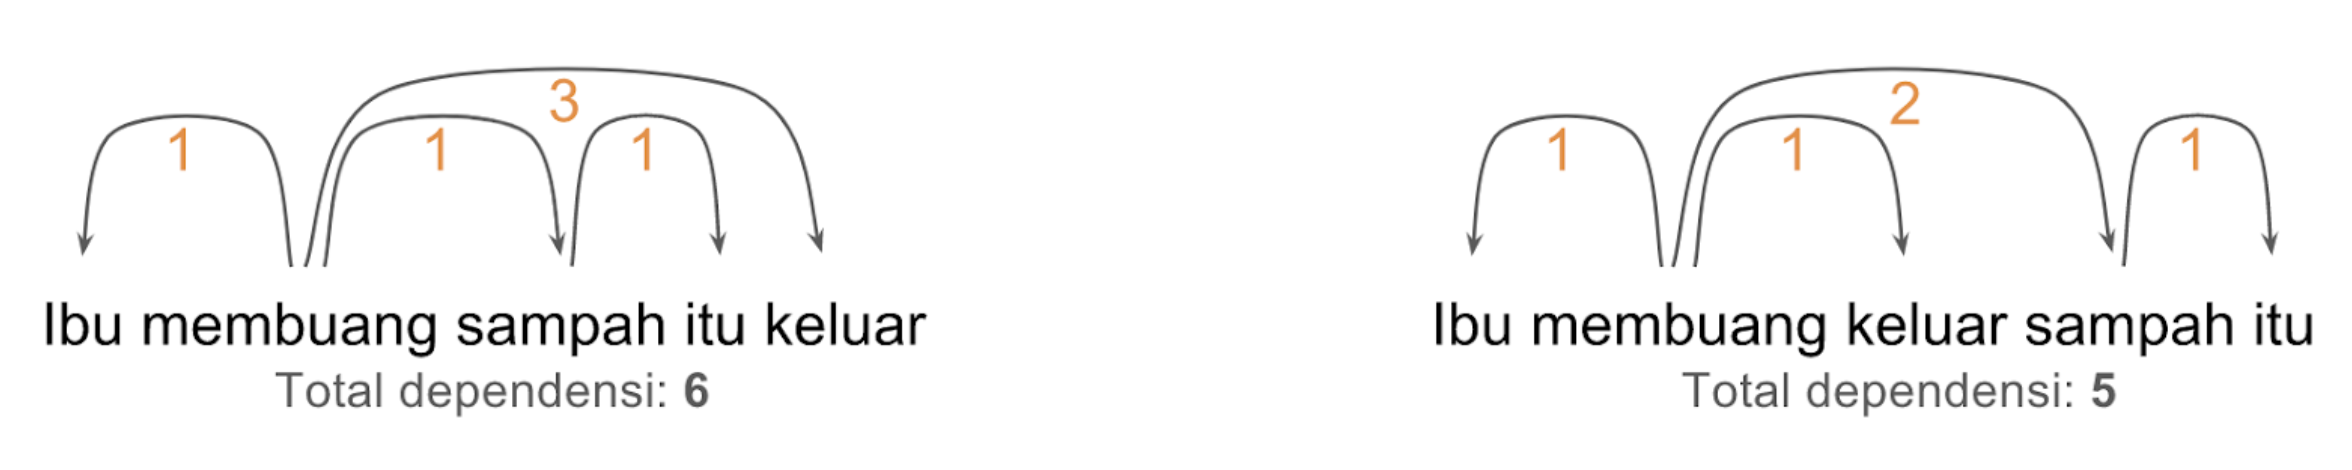
\includegraphics[width=1
	\textwidth] {pics/contoh-dependensi.png} \caption{Contoh perbedaan dependensi dalam bahasa Indonesia} 
\label{fig:contoh-dependensi} \end{figure}

Salah satu hipotesis yang membahas panjang dan jarak dependensi menyebutkan adanya kecenderungan bahwa penutur akan mendekatkan kata-kata yang memiliki relasi secara semantik dalam kalimat (\citealp{futrell2015large, liu2017dependency}). Hipotesis ini sangat berkaitan dengan prinsip efisiensi yang dikembangkan oleh \cite{hawkins2004efficiency}. Kata-kata yang mendekat mengakibatkan pengurangan panjang atau jarak dependensi sehingga berkaitan juga dengan hipotesis bahwa penutur cenderung lebih sulit dalam memproduksi dan memahami kalimat yang memiliki jarak dependensi yang jauh dan struktur yang rumit (\citealp{hawkins2004efficiency, dillon2011structured}). Sebagai contoh, pada \pic~\ref{fig:contoh-dependensi}, kata \textit{membuang} dan \textit{keluar} memiliki tautan langsung sehingga memori kerja penutur akan bekerja untuk menghubungkan keduanya. Semakin jauh jarak keduanya, semakin banyak memori kerja bekerja. Konsep tersebut mendukung penelitian \cite{jaeger2006redundancy} yang mengungkapkan bahwa penutur cenderung mengutamakan alasan efisiensi memori menyusun kata-kata dalam urutan linear pada sumbu sintagmatik, terutama pada ujaran yang lebih spontan \citep{jaeger2006redundancy}. \cite{futrell2015large} menemukan adanya fenomena pengurangan panjang dependensi antarkonstituen dalam 37 bahasa yang termasuk di dalamnya adalah bahasa Indonesia. Dalam penelitian tersebut, \cite{futrell2015large} menyebutkan bahwa temuan dalam bahasa Indonesia menunjukkan tingkat pengurangan panjang yang paling tinggi dibandingkan 36 bahasa lainnya. 

Penelitian terdahulu dengan data bahasa Indonesia yang membahas dependensi (\citealp{kamayani2011dependency, green2012indonesian, irmawati2015dependency, futrell2015large}) memanfaatkan korpus bahasa Indonesia yang mencakup data ragam tulis dari media jurnalistik daring, blog, artikel penelitian, dan media sosial. Pemilahan data dalam penelitian-penelitian tersebut hanya didasarkan pada keragaman dan kuantitas data. Berdasarkan hasil temuan \cite{wang2017effects}, \textit{genre} atau aliran teks hampir tidak berpengaruh terhadap pola distribusi jarak antarkonstituen yang memiliki relasi semantik. Hal ini berarti terlepas dari aliran teks, manusia cenderung untuk meminimalisir jarak dependensi pada kondisi tertentu \citep{wang2017effects}. Di lain sisi, \citep{wang2017effects} menemukan bahwa teks imajinatif cenderung memiliki jarak dependensi yang lebih panjang dibandingkan dengan teks informatif sehingga teks informatif lebih mudah untuk dimengerti\footnote{Penelitian \cite{wang2017effects} memanfaatkan British National Corpus yang mencakup teks informatif seperti berita dan laporan penelitian serta teks imajinatif seperti literatur fiksi dan dialog film.}. Namun, \cite{miller2011critical} mengkaji adanya perbedaan kerumitan sintaktis dalam teks informatif itu sendiri, seperti halnya media cetak formal akan lebih kompleks dibandingkan dengan artikel tabloid. Hal ini menunjukkan bahwa data penelitian linguistik terkait dependensi dapat difokuskan kepada salah satu aliran teks (informatif atau imajinatif) dan tetap mendapatkan gambaran keragaman pola yang ada di dalamnya. Keterbatasan lain yang dihadapi apabila melibatkan data bahasa sehari-hari (informal) adalah kurangnya sumber daya teknologi untuk mengolah data tersebut \citep{green2012indonesian}. 

Dalam banyaknya pembahasan mengenai efisiensi kalimat dipandang dari segi dependensi dalam linguistik secara global, terdapat kerumpangan terkait ranah tersebut dalam bahasa Indonesia. Kajian-kajian terdahulu yang menyinggung teori dependensi untuk bahasa Indonesia dilakukan oleh para peneliti terbatas untuk mengembangkan perangkat atau metode komputasional untuk penguraian kalimat berdasarkan dependensinya (\citealp{kamayani2011dependency, green2012indonesian, irmawati2015dependency}). Teori dependensi meninjau relasi semantik antara dua konstituen dalam sebuah kalimat, sehingga tidak terbatasi oleh relasi struktural. Oleh karena itu, teori dependensi merupakan dasar yang tepat untuk mengkaji ujaran nyata yang mungkin tidak memiliki struktur kalimat yang gramatikal, terutama pada bahasa-bahasa yang memiliki urutan kata bebas seperti bahasa Indonesia. Penelitian yang dapat memberikan wawasan dari aspek linguistik dengan teori dependensi akan sangat bermanfaat untuk kajian sintaksis modern terhadap bahasa Indonesia yang perkembangannya sangat alami dan cepat. Hingga saat ini, belum ada kajian dari aspek linguistik yang dapat memberikan wawasan tentang bagaimana konstruksi kalimat dapat menggambarkan efisiensi terkait panjang dan jarak dependensi dalam bahasa Indonesia. Sehubungan dengan kerumpangan tersebut, belum ada juga kajian yang memanfaatkan bukti penampilan bahasa berupa ujaran yang lebih spontan seperti data ragam lisan sebagai salah satu data utama penelitian. 

%-----------------------------------------------------------------------------%
\section{Perumusan masalah}
%-----------------------------------------------------------------------------%
Urutan kata dalam kalimat pada bahasa Indonesia tidak terkekang oleh aturan konstruksi dibandingkan dengan bahasa lain seperti Inggris dan Jerman (\citealp{stack2005word, futrell2015large, irmawati2015dependency}). \cite{kubler2009dependency} menyebutkan bahwa teori dependensi sangat sesuai untuk dimanfaatkan dalam menelaah bahasa dengan karakter urutan kata yang bebas seperti bahasa Indonesia. Tingginya tingkat pengurangan panjang dependensi kalimat yang ditemukan dalam bahasa Indonesia \citep{futrell2015large} juga menimbulkan pertanyaan mengenai keragaman pola pengurangan panjang dependensi kalimat serta jarak dependensi antarkonstituen dalam bahasa Indonesia itu sendiri.

Terkait dengan latar belakang di atas, muncul satu pokok permasalahan yang diuraikan dalam penelitian ini yaitu \textbf{bagaimana stuktur kalimat bahasa Indonesia ragam tulis dan lisan disusun secara efisien ditinjau dari segi dependensinya}. Dengan memanfaatkan korpus data jurnalistik bahasa Indonesia termutakhir ragam tulis dan lisan, pokok permasalahan ini diuraikan menjadi tiga pertanyaan yang lebih detail:

\begin{enumerate}
	\item Bagaimana pengaruh panjang kalimat terhadap penyusunan struktur kalimat yang efisien dalam bahasa Indonesia ragam tulis dan lisan dari segi dependensi? Pertanyaan ini dapat dinyatakan dalam bentuk hipotesis sebagai berikut \\
	$H_{1}A$ : Ada pengaruh panjang kalimat terhadap konstruksi kalimat dari segi dependensi. \\
	$H_{0}A$ : Tidak ada pengaruh panjang kalimat terhadap konstruksi kalimat dari segi dependensi.
	\item Bagaimana efisiensi kalimat tercermin pada panjang, jarak dan arah dependensi (direksionalitas induk) dalam bahasa Indonesia ragam tulis dan lisan? Pertanyaan ini dapat dinyatakan dalam bentuk hipotesis sebagai berikut \\
	$H_{1}B$ : Ada kecenderungan dalam bahasa Indonesia bahwa induk menempati posisi sebelum konstituen terikatnya dari segi dependensi. \\
	$H_{0}B$ : Tidak ada kecenderungan dalam bahasa Indonesia terkait posisi induk dan konstituen terikatnya.
	\item Bagaimana pengaruh penyusunan struktur kalimat yang efisien dalam bahasa Indonesia ragam tulis dan lisan dari segi dependensi terhadap valensi akar (\textit{root})?
\end{enumerate}

%-----------------------------------------------------------------------------%
\section{Tujuan penelitian}
%-----------------------------------------------------------------------------%
Penelitian ini memiliki tiga tujuan utama terkait pokok permasalahan penelitian. Pertama, penelitian ini bertujuan untuk meninjau pengaruh panjang kalimat terhadap struktur kalimat yang efisien dalam bahasa Indonesia ragam tulis dan lisan dari segi dependensi dengan memaparkan bukti empiris berdasarkan korpus data yang dikumpulkan. Kedua, penelitian ini memiliki tujuan untuk memperlihatkan bagaimana panjang, jarak dan arah dependensi (direksionalitas induk) dapat memberikan gambaran mengenai efisiensi kalimat dalam bahasa Indonesia ragam tulis dan lisan melalui analisis terhadap struktur sintaktis kalimat. Tujuan terakhir dari penelitian ini adalah untuk meninjau pengaruh struktur kalimat terhadap valensi akar (\textit{root}) kalimat tersebut dari segi dependensi.

Dalam mencapai tujuan-tujuan tersebut, beberapa aspek sintaksis terkait pembentukan struktur kalimat ini diuraikan untuk menguji hipotesis pengurangan panjang dan jarak dependensi antarkonstituen dalam sebuah kalimat seperti yang telah dibahas oleh beberapa penelitian terdahulu. Hasil penelitian ini berupa gambaran umum pengurangan panjang dan jarak dependensi pada beberapa aspek pembentukan struktur kalimat dan uraian secara mendalam mengenai tautan-tautan dependensi yang terjadi antara induk dan konstituen terikatnya. Penelitian ini menitikberatkan pada analisis penampilan bahasa (\textit{linguistic performance}) dengan memanfaatkan data penggunaan bahasa Indonesia secara nyata sebagaimana tercermin dalam korpus jurnalistik bahasa Indonesia ragam tulis dan lisan.

%-----------------------------------------------------------------------------%
\section{Manfaat penelitian}
%-----------------------------------------------------------------------------%
Jika penyusunan struktur kalimat yang digunakan penutur baik dari segi produksi maupun pemahaman didorong oleh motivasi untuk menurunkan kadar kesulitan berkomunikasi, maka ekspektasi utamanya adalah penghindaran terhadap tautan dependensi yang jauh \citep{futrell2015large}. Hipotesis pengurangan panjang dan jarak dependensi ini dapat berperan sebagai kerangka untuk menjelaskan hubungan antara bagaimana penutur memanfaatkan dan menyusun struktur sintaksis dalam sebuah bahasa dengan tujuan utama untuk menciptakan komunikasi yang efisien meskipun dengan menggunakan kalimat yang bersifat kompleks.

Secara teoretis, penelitian ini dapat menjadi dasar pengembangan ilmu sintaksis modern yang kontekstual karena menitikberatkan pada penampilan bahasa yang menjadi bukti empiris atas pemahaman kemampuan bahasa. Bukti-bukti penampilan bahasa dalam penelitian ini juga dapat ditindaklanjuti untuk merumuskan pengajaran ilmu sintaksis yang responsif terhadap penggunaan bahasa yang nyata dalam masyarakat. Selain itu, penelitian ini dapat dimanfaatkan oleh bidang perencanaan bahasa untuk memaknai penggunaan bahasa dalam masyarakat berdasarkan urutan kata dalam kalimat terkait dengan perkembangan relasi sintagmatik pada periode waktu data penelitian untuk ragam tulis dan lisan. Dalam kajian kesemestaan bahasa (\textit{language universals}), penelitian ini turut menyumbangkan gambaran mendalam terkait penampilan bahasa Indonesia dalam ranah dependensi.

Secara praktis, penelitian ini dapat memberikan kontribusi terhadap pengembangan perangkat metode linguistik komputasional dan pemrosesan bahasa alami. Kontribusi tersebut berupa wawasan tentang kajian penampilan bahasa Indonesia dalam perspektif dependensi, terutama terkait bahasa Indonesia ragam lisan yang hingga saat ini masih sangat jarang dimanfaatkan dalam pemrosesan bahasa secara digital. Temuan mengenai kaitan struktur dependensi yang memudahkan komunikasi dapat menjadi acuan utama untuk kerangka kerja dalam pemrosesan bahasa alami atau \textit{Natural Language Processing} (NLP). Seperti yang dibahas dalam penelitian \cite{klein2004corpus} serta \cite{smith2006minimum}, beberapa model komputasi termutakhir memanfaatkan asumsi pengurangan jarak dependensi untuk mereplika penggunaan bahasa oleh penutur dan hasilnya lebih mendekati ujaran nyata (\textit{real utterance}).

%-----------------------------------------------------------------------------%
\section{Batasan penelitian}
%-----------------------------------------------------------------------------%
Pada dasarnya, penelitian ini melihat bagaimana konstruksi atau struktur kalimat yang efisien dari segi dependensi. Dalam teori linguistik lain, efisiensi sebuah bahasa sering dikaitkan dengan bagaimana penutur berusaha untuk 'menghemat' tenaga dalam ujaran nyata terutama dengan memperpendek tuturan-tuturannya. Penghematan ini disebut juga dengan 'ekonomi bahasa' yang termasuk didalamnya adalah penghilangan fonem dan abreviasi \citep{verhaar1996asas}. Namun, perlu ditekankan bahwa aspek efisiensi yang dimaksud dalam penelitian ini dibatasi pada efisiensi dari segi pemrosesan terkait memori kerja pada ranah sintaksis \citep{hawkins2014cross}. Data observasi yang digunakan dalam penelitian ini merupakan kumpulan ujaran nyata yang tergabung pada korpus jurnalistik bahasa Indonesia ragam tulis dan lisan dalam rentang tahun publikasi atau rekaman dari 2008 hingga 2018. Dengan menggunakan data dari berbagai media nasional dan daerah yang menggunakan bahasa Indonesia, penelitian ini membedah struktur dan susunan kata pada tataran kalimat dengan menggunakan metode-metode yang dikembangkan berdasarkan teori dependensi yang pertama dikemukakan oleh \cite{tesniere1959elements}. 

\citet[pp. 3-5]{tesniere1959elements} menyebutkan bahwa kalimat merupakan sebuah susunan terorganisir yang memiliki konstituen berupa unit-unit kata. Organisasi konstituen dalam kalimat ini dihasilkan oleh relasi-relasi yang terbentuk antarkonstituen. Terkait dengan relasi yang muncul dalam sebuah kalimat, perlu ditekankan bahwa tidak semua relasi antarkonstituen dalam kalimat merupakan dependensi. Sebagai contoh, relasi antara kata \textit{ayah} dengan \textit{Pak Yahya} dalam kalimat \textit{Saat Budi melihat sang ayah, Pak Yahya sedang membawa adiknya pergi} bukan merupakan dependensi. Dalam kalimat tersebut, \textit{ayah} dan \textit{Pak Yahya} adalah orang yang sama sehingga memiliki relasi berupa acuan. Oleh karena itu, penelitian ini membatasi ruang lingkup relasi hanya pada relasi semantik terkait teori dependensi yang dijabarkan oleh \cite{tesniere1959elements}. Implikasi dari penelitian ini, sesuai dengan permasalahan yang diangkat, adalah pemaparan kecenderungan terkait panjang, jarak dan arah dependensi (direksionalitas induk), penelusuran pengaruh panjang kalimat terhadap strategi efisiensi kalimat dipandang dari segi dependensi, dan eksplorasi pengaruh strategi urutan kata terhadap valensi sebuah kata berdasarkan korpus yang diteliti. 

Untuk mencapai implikasi yang diharapkan, penelitian ini menggabungkan ancangan kuantitatif dan kualitatif. Ancangan kuantitatif berupa penguraian kalimat berdasarkan dependensinya (\textit{dependency parsing}), penghitungan statistika deskriptif untuk mendapatkan paparan pola struktur kalimat, dan percobaan acak dengan mengadopsi pendekatan Dasar Urutan Kata Bebas atau \textit{Free Word Order Baseline} yang digunakan oleh \cite{futrell2015large}. Penguraian kalimat berdasarkan dependensi dilakukan dengan menggunakan dasar bank pohon struktur dependensi atau \textit{dependency treebank} dalam Universal Dependencies 2.0 \citep{nivre2017universal} yang telah dikondisikan untuk bahasa Indonesia. Penghitungan statistika deskriptif untuk mendapatkan paparan pola jarak dan arah dependensi serta tes signifikansi pengaruh panjang kalimat terhadap struktur kalimat dilakukan dengan mengadopsi pendekatan yang digunakan oleh \cite{gildea2010grammars}, \cite{futrell2015large}, \cite{jiang2015effects} dan \cite{liu2017dependency}. Ancangan kuantitatif ini tidak mengukur tingkat efisiensi sebuah kalimat ataupun seberapa besar optimasi struktur sebuah kalimat dari segi pengurangan panjang dan jarak dependensi. Proses yang dibutuhkan untuk mencapai kedua tujuan ini membutuhkan pengetahuan dan metode yang berada pada ranah ilmu kognitif. Sementara itu, ancangan kuantitatif ini memiliki tujuan utama untuk untuk menguji hipotesis pengurangan panjang dan jarak dependensi pada tataran kalimat dengan memanfaatkan korpus data yang dikumpulkan dan memberikan gambaran pola-pola struktur sintaksis yang banyak muncul untuk dianalisis secara kualitatif.

Ancangan kualitatif diterapkan untuk melanjutkan hasil analisis yang didapat dari pendekatan kuantitatif. Pendekatan ini digunakan untuk menguraikan lebih dalam efisiensi kalimat terutama terkait direksionalitas induk atau  arah dependensi, perbandingan strategi struktur sintaktis pada klasifikasi berdasarkan panjang kalimat, serta struktur sintaktis kalimat yang terbentuk akibat perubahan valensi akar verbal yang diduga muncul dalam bahasa Indonesia. Seluruh ancangan kualitatif ini dilakukan pada tataran kalimat. Dalam teori dependensi, kalimat dianalogikan sebagai pertunjukan teater dengan adanya aktor (\textit{actants}), proses (\textit{verbs}), dan situasi (\textit{circumstants}) yang di setiap kalimat memiliki simpai pusat (\textit{central node}) sebagai pengendali keseluruhan kalimat \citep{tesniere1959elements}. Mengacu pada konsep ini, pendekatan kualitatif untuk melihat perubahan valensi dibatasi hanya pada simpai pusat (\textit{central node}) pada kalimat-kalimat yang mewakili pola terbanyak, yaitu kalimat yang memiliki akar berupa kata kerja atau verba. Analisis kualitatif ini menggunakan kerangka kerja tata bahasa kata (\textit{Word Grammar}) yang dikembangkan oleh (\citealp{hudson1984word,hudson2007language}). Gabungan kedua ancangan ini diharapkan dapat memberikan gambaran makro dan mikro secara sistematis dan terperinci terhadap efisiensi bahasa terkait susunan kata dalam kalimat dipandang dari segi dependensi. 



%-----------------------------------------------------------------------------%
\section{Kerangka konseptual}
%-----------------------------------------------------------------------------%
Kerangka konseptual penelitian ini melibatkan beberapa elemen dan proses mulai dari pengumpulan dan persiapan dalam membentuk korpus data ragam tulis dan lisan, pengolahan data, hingga analisis data yang melibatkan ancangan kuantitatif (percobaan acak dan agregasi data) serta ancangan kualitatif (analisis struktur sintaksis pada simpai pusat). Berikut dijabarkan keseluruhan elemen dan proses yang terlibat dalam penelitian ini:

\begin{enumerate}
	\item Data jurnalistik termutakhir dalam bahasa Indonesia yang dipisahkan menjadi kumpulan teks atau korpus (\textit{corpus}) data ragam tulis dan korpus data ragam lisan. Data jurnalistik dapat mewakili aliran penggunaan bahasa yang cukup formal untuk dapat diproses melalui metode komputasional, namun juga cukup memberikan ruang untuk penuturnya dalam berkreasi membentuk struktur kalimat tersendiri. Persiapan korpus data ragam lisan melibatkan tahapan tambahan berupa transkripsi otomatis dengan Google Speech API dan pemeriksaan secara manual untuk memastikan kualitas transkripsi. Kedua korpus juga melalui pemeriksaan secara manual untuk memastikan kalimat-kalimat tidak lengkap tidak ikut dalam proses analisis. Kedua korpus data ini merupakan masukan (\textit{input}) utama penelitian ini.
	\item Persiapan kalimat yang diekstraksi dari kedua korpus data ini merupakan tahap persiapan utama untuk dapat melalui pengolahan data dengan memanfaatkan penguraian kalimat berdasarkan dependensinya. Pemisahan ini dilakukan mengingat penelitian ini memiliki ruang lingkup pada tataran kalimat. Persiapan untuk memisahkan semua kalimat dari wacana-wacana dalam kedua korpus ini melibatkan proses otomatis dan pemeriksaan secara manual untuk memastikan kualitas data yang sesuai ekspektasi. 
	\item Ancangan kuantitatif yang melibatkan agregasi data untuk mendapatkan nilai-nilai yang dapat digunakan dalam tinjauan pengurangan panjang dan jarak dependensi serta aspek-aspek lain sesuai dengan permasalahan penelitian. Termasuk di dalam proses ini adalah percobaan acak dengan pendekatan \textit{Free Word Order Baseline} yang menjadi dasar utama pembuktian adanya pengurangan panjang dan jarak dependensi pada tataran kalimat.
	\item Ancangan kualitatif bertitik tolak dari temuan pendekatan kuantitatif yang menghasilkan indikasi-indikasi pola struktur sintaksis menggambarkan strategi untuk pengurangan panjang dan jarak dependensi. Ancangan ini melibatkan analisis terhadap struktur sintaksis kalimat dengan akar (\textit{root}) berupa verba pada simpai pusat. 
	\item Luaran dari penelitian ini berupa hasil tinjauan terhadap pengurangan panjang dan jarak dependensi serta indikasi strategi pengurangan panjang dan jarak dependensi terkait beberapa aspek struktur sintaktis. Aspek-aspek ini meliputi panjang kalimat, konstruksi kalimat yang berpengaruh terhadap panjang, jarak dan arah dependensi, serta perubahan valensi verbal pada simpai pusat.
\end{enumerate}

\newpage
Berikut adalah ilustrasi kerangka konseptual yang secara keseluruhan diterapkan dalam penelitian ini (\pic~\ref{fig:kerangka-konseptual}). 
\begin{figure}
	\centering 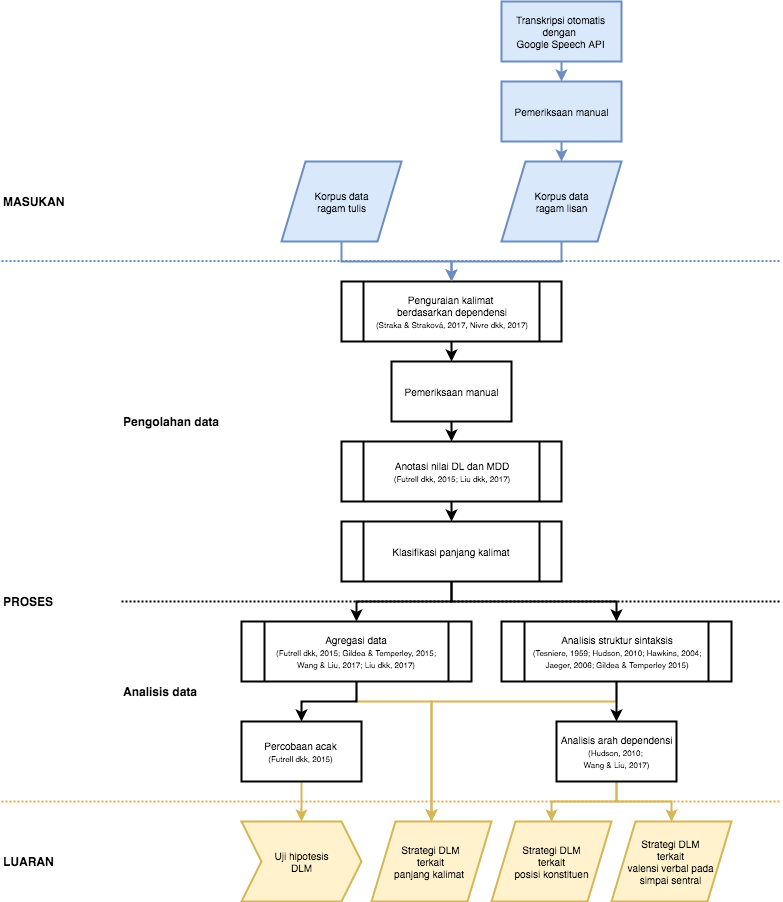
\includegraphics[width=1
	\textwidth] {pics/kerangka-konseptual.png} \caption{Diagram alur kerangka konseptual penelitian} 
\label{fig:kerangka-konseptual} \end{figure}

Berdasarkan kerangka konseptual yang telah disusun, beberapa teori dan luaran dari penelitian-penelitian terdahulu diperlukan untuk menjadi dasar kerangka teoretis penelitian tesis ini. Aspek teoretis dari kerangka konseptual tersebut dijabarkan sebagai berikut:
\begin{itemize}
	\item Spontanitas ujaran terutama dalam bahasa Indonesia menjadi dasar utama dalam menentukan jenis data yang digunakan sebagai obyek penelitian.
	\begin{itemize}
		\item Spontanitas ujaran merupakan aspek utama yang mendasari pemilihan korpus jurnalistik ragam tulis dan lisan. Dasar teoretis yang digunakan untuk mendukung perbedaan kedua ragam ini adalah variasi dan perbedaan sintaktis antara ujaran lisan dan tulisan berdasarkan pembahasan \cite{biber1991variation} dan \cite{o1974syntactic}.
		\item Teori sintaksis deskriptif yang dijabarkan oleh \cite{kridalaksana1999deskriptif, kridalaksana2002struktur} dan \textit{Indonesian Reference Grammar} \citep{sneddon2010indonesian} merupakan dasar teoretis pada aspek ketatabahasaan dalam bahasa Indonesia.
	\end{itemize}
	\item Konsep dependensi yang mendasari pendekatan penguraian kalimat berdasarkan dependensi serta penghitungan panjang dan jarak dependensi.
	\begin{itemize}
		\item Pembahasan elemen-elemen yang membentuk sebuah tautan dependensi seperti akar, induk, konstituen terikat, dan simpai menggunakan dasar teoretis dari  \cite{tesniere1959elements} yang kemudian dikembangkan oleh \cite{heringer1993dependency} dan \cite{hudson2010introduction}.
		\item Indikator panjang dan jarak dependensi yang dikembangkan oleh \cite{liu2017dependency} dan \cite{gildea2010grammars} menjadi dasar pembahasan untuk kuantifikasi atau penghitungan tautan dependensi dan anotasi panjang dan jarak dependensi pada setiap kalimat.
		\item Beberapa luaran penelitian yang dilakukan oleh \cite{gibson1998linguistic}, \cite{hiranuma1999syntactic}, \cite{liu2009chinese}, dan \cite{wang2017effects} mengenai pengaruh panjang kalimat dan jenis teks terhadap dependensi digunakan sebagai acuan klasifikasi kalimat terkait faktor-faktor yang mempengaruhi tautan dependensi.
	\end{itemize}
	\item Dasar proses analisis untuk melihat efisiensi kalimat dari segi dependensi melalui percobaan acak dan analisis kualitatif struktur sintaktis yang telah diuraikan berdasarkan dependensinya.
	\begin{itemize}
		\item Pengurangan panjang dependensi (\citealp{temperley2007minimization, temperley2008dependency, gildea2010grammars}), pengurangan jarak dependensi (\citealp{liu2008dependency, liu2017dependency}) dan pembahasan efisiensi kalimat terkait memori kerja \citep{hawkins2004efficiency} digunakan sebagai hipotesis yang mendasari analisis efisiensi kalimat dari segi dependensi melalui percobaan acak.
		\item Beberapa dasar teoretis digunakan sebagai dasar analisis kualitatif terhadap tautan dependensi mengenai tingkat kedalaman struktur sintaktis \citep{yngve1960model}, posisi induk terhadap konstituen terikat atau direksionalitas induk (\citealp{dryer1992greenbergian, temperley2008dependency}), dan valensi pada simpai pusat akar verbal (\citealp{hudson2007language, welke2002deutsche})
	\end{itemize}
\end{itemize}
	
%-----------------------------------------------------------------------------%


%-----------------------------------------------------------------------------%
\chapter{\babDua}
%-----------------------------------------------------------------------------%

%-----------------------------------------------------------------------------%
\section{Konteks penelitian}
%-----------------------------------------------------------------------------%
Kalimat merupakan sebuah susunan terorganisir yang memiliki konstituen berupa kata dan tanda baca. Makna semantis sebuah konstituen di dalam ujaran atau kalimat tidak berdiri sendiri seperti konstituen-konstituen dan maknanya yang tertulis di dalam kamus. Melainkan, dalam penggunaan bahasa secara nyata, makna setiap konstituen tersebut baru akan terbentuk utuh setelah memiliki relasi dengan konstituen lain dalam sebuah frasa, klausa, kalimat maupun paragraf. Pembentukan relasi sebuah konstituen dengan konstituen lain ini merupakan salah satu hasil penerapan fungsi konstituen \citep{tesniere1959elements}. Dalam ruang lingkup dependensi, fungsi yang membentuk relasi antarkonstituen dalam struktur kalimat tersebut terbagi dua: fungsi sintaksis (struktural) dan fungsi semantik (makna) \citep{tesniere1959elements}. Meskipun sintaksis dan semantik adalah dua bidang yang independen dan berbeda, keduanya masih berjalan sejajar dan saling berhubungan dalam teori dependensi \citep{tesniere1959elements}. Hal ini terjadi karena dependensi merupakan tautan struktural langsung yang menghubungkan unit-unit linguistik yang memiliki relasi semantik. Dalam perkembangan teorinya, konsep dependensi ini dapat dilacak jejaknya hingga pada penerapan tata bahasa Panini \citep{bharati1995natural}, tata bahasa Yunani dan Latin kuno (\citealp{covington1984syntactic, percival1990reflections}), serta tata bahasa Arab \citep{owens1988foundations}. 

Konsep dependensi yang ditemukan pada beberapa tata bahasa kuno di atas menunjukkan bahwa kata merupakan konstitituen atau unit utama sintaksis dan konstituen-konstituen dalam kalimat tersebut memiliki relasi struktural secara langsung. \citet{hudson1984word, hudson2007language} mengembangkan teori \textit{Word Grammar} atau Tata Bahasa Kata yang menjelaskan tentang peran kata, kesejajaran, dan hubungan antara sintaksis (struktur) dan semantik (makna). \textit{Word Grammar} mengadopsi konsep dependensi sebagai dasar untuk menelaah struktur kalimat dan melihat bahasa sebagai sebuah jejaring \citep{hudson2007language}. Kata sebagai unit utama sintaksis dan penerapannya dalam teori dependensi juga banyak menjadi bahan pembahasan dalam pengembangan metode komputasional. Salah satu teori utama terkait linguistik komputasional yang bertitik tolak dari teori dependensi tersebut adalah \textit{Meaning-Text Theory} atau Teori Makna-Teks (MTT) yang dikembangkan oleh \cite{mel'vcuk1988dependency} dan penguraian kalimat multilingual berdasarkan teori dependensi yang dibangun dari pengumpulan data bank pohon struktur dependensi dari berbagai bahasa, proyek ini disebut dengan \textit{Universal Dependencies} (\citealp{mcdonald2013universal, nivre2016universal, nivre2017universal}). 

Adanya bukti-bukti dependensi yang ditemukan secara lintas bahasa merupakan indikasi utama bahwa fenomena ini dialami beberapa atau bahkan semua bahasa di dunia (universal). Asumsi bahwa dependensi bersifat universal menandakan keterkaitan konsep ini dengan kerja kognisi manusia \citep{gibson2000dependency}. Salah satu isu utama dalam memahami bagaimana pengetahuan bahasa diimplementasikan di dalam kognisi manusia melibatkan kajian terhadap produksi dan pemahaman bahasa menggunakan data tuturan nyata. Pengetahuan di dalam kognisi manusia terkait aturan yang membentuk sebuah bahasa ini disebut dengan 'kemampuan' (\textit{competence}). Sementara itu, aktivitas kebahasaan yang memanfaatkan pengetahuan tersebut secara nyata disebut dengan 'penampilan' (\textit{performance}) \citep{delahuntygarvey2010soundsense}. Beberapa studi berdasarkan bukti-bukti penampilan menunjukkan bahwa dalam mengkonstruksikan sebuah struktur kalimat, penutur melibatkan proses memori kerja secara bertahap (\textit{moment-by-moment}) \citep{gibson2000dependency}. Hubungan memori kerja secara bertahap dengan konstruksi kalimat menggambarkan bagaimana produksi dan pemahaman kalimat dipengaruhi pertimbangan untuk memudahkan proses memori kerja \citep{futrell2015large}. Berkaitan dengan asumsi tersebut, muncul hipotesis adanya kecenderungan bahwa penutur akan mendekatkan konstituen-konstituen dalam kalimat yang memiliki relasi secara semantik (digambarkan melalui \gls{tautan-dependensi} yang menghubungkan kedua konstituen tersebut) (\citealp{futrell2015large, liu2017dependency}). Konstituen-konstituen yang mendekat ini juga dikaitkan dengan hipotesis bahwa penutur cenderung lebih sulit dalam memproduksi dan memahami kalimat dengan panjang atau jarak dependensi yang jauh dan struktur yang rumit (\citealp{gibson2000dependency, dillon2011structured}).

Hubungan erat antara struktur kalimat dengan penyimpanan memori dan proses memori kerja menimbulkan pertanyaan mengenai pola dependensi pada kalimat dengan derajat spontanitas yang tinggi seperti pada ragam lisan \citep{abney1991memory}. Pertanyaan ini menjadi dasar pemilihan kedua korpus data ragam tulis dan lisan untuk analisis dependensi terkait derajat spontanitas kalimat dan jenis ujaran. Selain itu, terdapat beberapa pembahasan yang menyoroti pengaruh faktor karakter bahasa dan ketatabahasaan terhadap pola dependensi (\citealp{hawkins2014cross, jiang2015effects, wang2017effects}). Meskipun tidak membahas faktor karakter bahasa dan ketatabahasaan, dalam penelitian lintas bahasa yang berskala besar, \cite{futrell2015large} menyebutkan bahwa temuan dalam bahasa Indonesia menunjukkan tingkat optimasi kalimat yang paling tinggi dibandingkan 36 bahasa lain dalam penelitiannya. Optimasi yang dimaksud adalah sejauh mana konstituen-konstituen dalam sebuah kalimat didekatkan. Sebagai contoh, perbandingan temuan optimasi terkait dengan urutan linear kata (\textit{word order}) antara bahasa Indonesia dengan Jerman dalam penelitian \cite{futrell2015large} sangat kontras. Tidak hanya terkait karakter dan ketatabahasaan dalam sebuah bahasa, perbedaan temuan mengenai analisis dependensi juga mungkin diakibatkan oleh perbedaan jenis teks yang dianalisis. Berkaitan dengan ini, \cite{wang2017effects} melakukan penelitian lintas bahasa yang menunjukkan adanya perbedaan jarak dependensi terutama antara teks yang bersifat informatif dan teks imajinatif.

Struktur sebuah kalimat memiliki relasi sintaktis yang diterapkan berkenaan dengan tata bahasanya, namun struktur tersebut juga mengandung relasi dari segi semantik. \cite{tesniere1959elements} menganggap tata bahasa yang menjadi ancangan relasi sintaktis ini sebagai sesuatu yang bersifat intrinsik karena merupakan sistematika yang mendasari sebuah kalimat. Relasi sintaktis ini memungkinkan makna sebuah kalimat untuk diproduksi secara utuh dan dipahami oleh penerima informasi. Oleh karena itu, relasi semantik yang tersampaikan kepada dan dipahami pendengar atau pembaca disebut sebagai hal yang ekstrinsik \citep{tesniere1959elements}. Keterkaitan fungsi sintaktis dan semantis ini juga muncul dalam hubungan antarkonstituen karena relasi semantik terintegrasikan ke dalam relasi sintaktis. \cite{tesniere1959elements} menyebut kesejajaran kedua fungsi ini dengan istilah 'struktur mengekspresikan makna' atau \textit{the structural expresses the semantic}. Hubungan ini dapat dinyatakan juga sebagai berikut: makna \gls{konstituen-terikat} membawa bersamanya kualitas induk tempatnya bergantung. Oleh karena itu, hierarki signifikansi konstituen secara struktural berbanding terbalik dengan semantik.

%-----------------------------------------------------------------------------%
\subsection{Dikotomi kemampuan dan penampilan bahasa}
%-----------------------------------------------------------------------------%
Intelektualitas untuk berkomunikasi dan berbahasa adalah kemampuan utama yang membedakan manusia dengan mahluk yang lain. Meskipun setiap daerah di seluruh dunia memiliki keunikan dalam berkomunikasi dan berbahasa, terdapat asumsi bahwa di balik perbedaan itu, ada kesamaan kualitas bahasa yang disebabkan oleh cara kerja kognisi manusia yang serupa \citep{sapir1921intro, chomsky1965syntactic}. \cite{beattie1788theory} merupakan salah satu orang pertama yang menjelaskan keunikan setiap bahasa terkait leksikon dan tata bahasanya. \cite{chomsky1965syntactic} menyanggah prinsip tata bahasa tradisional yang mengatakan bahwa 'susunan alami pikiran' \textit{natural order of thoughts} sudah pasti tercermin pada urutan kata dalam sebuah kalimat yang dibahas dalam konvensi tata bahasa. Sebagai contoh, \cite{diderot1751lettre} beranggapan bahwa bahasa Perancis merupakan salah satu bahasa yang urutan kata dalam kalimatnya berkorespondensi terhadap susunan alami pikiran dan ide. Hal ini berarti bagaimanapun susunan yang terbentuk dalam bahasa tersebut baik dalam periode kuno maupun modern, pikiran dan ide penutur dapat dianalisis secara semantik dengan mengikuti norma-norma sintaksisnya. Namun, salah satu aspek dari teori-teori linguistik tradisional yang masih relevan dalam teori-teori linguistik modern adalah bahwa terdapat setidaknya satu karakter yang mengaitkan seluruh bahasa di dunia, yaitu dalam aspek kreativitas dan variasinya \citep{hawkins2014cross}.

Bahasa memiliki sarana terbatas (\textit{finite means}) dan keterbatasan (\textit{constraints}) dalam berbagai aspek \citep{von1972origin}. \cite{von1972origin} menyampaikan ini dalam kalimat "\textit{make use of make infinite use of finite means}" untuk menggambarkan kemampuan sebuah bahasa terkait aspek kreativitas dan variasinya. Studi mengenai keterbatasan dan bagaimana bahasa mengakali keterbatasan tersebut telah berkembang selama puluhan tahun terakhir, termasuk di dalamnya adalah kajian berbasis data penampilan bahasa dengan mengintegrasikan ilmu linguistik dan prinsip-prinsip dalam matematika \citep{chomsky1965syntactic}. Semenjak adanya rintisan hasil kerja dari \cite{chomsky1957syntactic}, dunia linguistik mulai mempertimbangkan tata bahasa sebagai perangkat formal berupa deskripsi eksplisit mengenai batasan-batasan produktif sebuah bahasa. Hal ini berarti tata bahasa membatasi berbagai kemungkinan formula yang terbentuk dari relasi antara satu konstituen (seperti kata atau morfem) dengan konstituen lain dalam kategori sintagmatik. Salah satu tujuan utama tata bahasa, menurut \cite{chomsky1965syntactic}, adalah untuk membedakan urutan konstituen yang gramatikal dengan yang tidak gramatikal\footnote{Pada pembahasan ini, bahasa yang dimaksud Chomsky dipandang sebagai bentuk urutan kata tidak terbatas yang masing-masing memiliki asosiasi relevan dengan deskripsi struktural tata bahasanya.}. Dari sini, \cite{chomsky1965syntactic} mengekspresikan tata bahasa sebagai kemampuan bahasa\footnote{Dalam Kamus Linguistik \citep{kridalaksana2008kamus}, kemampuan bahasa dijabarkan sebagai "kemampuan bahasawan untuk memahami dan menghasilkan kalirnat-kalimat yang belum pernah didengar sebelumnya, yakni kode yang mendasari semua ujaran dalam satu bahasa". Sementara, penampilan bahasa dijabarkan sebagai "realisasi kode itu dalam pemakaian bahasa yang sebenarnya, yakni ujaran itu sendiri".} (\textit{linguistic competence}) yang berarti pengetahuan penutur/pendengar terhadap bahasanya. Dalam kemampuan bahasa, istilah 'gramatikal' menjadi salah satu tolok ukur. \cite{chomsky1965syntactic} menegaskan perbedaan antara istilah tersebut dengan 'dapat diterima' atau \textit{acceptable}. Berbeda dengan konsep 'gramatikal', keterterimaan (\textit{acceptability}) merupakan konsep dan tolok ukur dalam studi penampilan bahasa (\textit{linguistic performance}) \citep{chomsky1965syntactic}. Studi terhadap penampilan bahasa merupakan studi terhadap penggunaan bahasa oleh penutur dalam situasi yang nyata dengan menggunakan tuturan nyata. Dikotomi\footnote{Dalam pandangan teknis, Chomsky melihat teori linguistik sebagai hal yang bersifat mentalistik karena berkenaan dengan penjajakan realitas mental yang mendasari perilaku nyata. Chomsky menekankan hal tersebut untuk membedakan dikotomi \textit{competence-performance} dengan \textit{langue-parole} yang dikemukakan Saussure \citep{key2017course}. Bagi Chomsky, \textit{langue} hanya mencakup inventori sistematis dari unit-unit linguistik. Dalam konteks realitas mental, kemampuan lebih dekat dengan konsepsi pemikiran dalam proses generatif yang digagas oleh \cite{von1972origin}.} yang digagas \cite{chomsky1965syntactic} ini berangkat dari hasil analisis yang menunjukkan bahwa kemampuan tidak selalu dapat tercermin secara langsung pada penampilan.

Perkembangan pembahasan mengenai dikotomi \textit{competence-performance} atau kemampuan-penampilan sangat menekankan pada hubungan kedua aspek tersebut. Salah satunya adalah \cite{sagwasow2011pccg} yang menyatakan bahwa teori-teori terkait kemampuan bahasa harus dapat menjadi basis model yang digunakan dalam menganalisis penampilan bahasa. Para linguis yang mendukung paham ini menambahkan bahwa peneliti dalam bidang teori gramatikal atau studi kemampuan bahasa seharusnya mengintegrasikan studi penampilan bahasa yang memanfaatkan tuturan nyata sehingga dapat berperan sebagai dasar bukti empiris untuk pengembangan ranah kemampuan bahasa. Hubungan antara kemampuan dan penampilan bahasa ini pertama diungkit oleh J.H. Greenberg (\citealp{greenberg1963some, greenberg1966language}) yang memperlihatkan pola korelasi antara temuan penampilan dan tata bahasa terkait evolusi dari aturan bahasa yang mungkin muncul dari penggunaan bahasa dalam keseharian secara terus-menerus (reguler). \cite{givon1979syntax} juga melakukan observasi bahwa kecenderungan pilihan (preferensi) penutur terhadap bentuk ujaran tertentu dalam sebuah bahasa mungkin berkorelasi dengan persyaratan kategoris (gramatikal). 

Perkembangan teori-teori lain yang berangkat dari dikotomi kemampuan-penampilan seperti Teori Optimalitas (\textit{Optimality Theory}) menghasilkan temuan adanya alasan fungsional yang mendasari batasan gramatikal dasar (\citealp{haspelmath1999optimality, aissen1999markedness}). Teori lain seperti Teori Optimalitas Stokastik (\textit{Stochastic Optimality Theory}) (\citealp{bresnan2001soft, manning2003probabilistic}) mengintegrasikan temuan kecenderungan pilihan atau preferensi yang didapatkan dari studi penampilan bahasa sebagai batasan lunak (\textit{soft constraints}) dan konvensi gramatikal sebagai batasan keras (\textit{hard constraints}). Gabungan kedua batasan ini menjadi salah satu penerapan praktis dalam upaya untuk mengaitkan kemampuan dan penampilan bahasa. Tidak hanya dalam ruang lingkup bahasa Indonesia, penelitian mengenai hubungan kedua aspek tersebut juga masih terus berkembang secara signifikan secara global karena masih banyak aspek yang harus digali terkait mekanisme adaptif\footnote{Mekanisme adaptif yang dimaksud adalah dasar mekanisme sebuah bahasa yang mungkin dimiliki oleh semua bahasa. Termasuk di dalam mekanisme ini adalah fleksibilitas tata bahasa terhadap kalimat yang tidak gramatikal, namun masih dapat diterima (\textit{acceptable}).} \citep{kirby1999function}. Berbagai pertanyaan dari mekanisme adaptif ini patut dipertimbangkan sebagai tujuan akhir dari penelitian-penelitian terkait, seperti pada titik mana konvensi gramatikal dapat terbentuk dari variasi yang dihasilkan penampilan bahasa, bagaimana proses model gramatikal dapat mengatur preferensi penampilan bahasa, serta apa yang dapat menjadi tolok ukur pertimbangan untuk penyaringan preferensi penampilan menjadi konvensi tata bahasa.


%-----------------------------------------------------------------------------%
\subsection{Efisiensi kalimat dan urutan kata dalam ranah ilmu sintaksis}
%-----------------------------------------------------------------------------%
Seperti yang dijelaskan sebelumnya, penelitian mengenai hubungan kedua aspek dikotomi kemampuan-penampilan banyak mencakup pertimbangan terbentuknya preferensi dalam studi penampilan bahasa dan konvensi gramatikal. Dalam ruang lingkup sintaksis, hal ini berkaitan dengan kemampuan sebuah bahasa yang dimiliki penutur untuk dapat berekspresi melalui variasi kalimat yang tidak terbatas meskipun dengan struktur yang terbatas (\citealp{von1972origin, plotkin2000language}). Konsep ini menggambarkan hubungan erat antara sintaksis dengan kognisi manusia yang menghasilkan pandangan-pandangan yang menganggap bahwa seiring waktu, bahasa dibentuk oleh batasan mekanisme kognisi manusia serta tekanan terkait akuisisi dan penggunaan bahasa \citep{plotkin2000language}. Berbagai gagasan yang diajukan terkait tekanan kognitif yang membatasi pembentukan struktur kalimat mencakup keterbatasan memori kerja \citep{slobin1973cognitive}, batasan atas pengolahan bahasa dan persepsi \citep{bever1970cognitive}, dan pertimbangan terhadap komunikasi yang efisien (\citealp{macwhinneybates1989cross, givon1991markedness, zipf1949human}). 

Berdasarkan pembahasan mengenai pembentukan struktur kalimat dan pertimbangan terhadap komunikasi yang efisien, \cite{hawkins2004efficiency} menemukan bahwa efisiensi yang dimaksud terintegrasikan dalam proses produksi dan pemahaman bahasa. Temuan ini memperlihatkan bahwa tata bahasa telah mengkonvensionalisasikan struktur kalimat sehingga proporsional terhadap preferensi pada studi penampilan bahasa \citep{hawkins2004efficiency}. Analisis ini didapatkan dengan memetakan pola seleksi dalam korpora dan eksperimen psikolinguistik untuk melihat kemudahan pengolahan bahasa. Kedua sumber data menunjukkan temuan yang serupa, yaitu adanya kecenderungan untuk memilih pronomina persona dalam klausa relatif pada lingkungan yang lebih kompleks sehingga efisiensi diraih dengan meminimalkan ranah (\textit{domain minimization}) \citep{hawkins2004efficiency}. Dalam konteks urutan konstituen, hal ini berarti frasa dan klausa harus dirakit menjadi kelompok-kelompok yang dapat direpresentasikan dengan diagram struktural, namun diproduksi dalam bentuk kalimat yang linear. Beberapa bentuk urutan kata dapat mereduksi jumlah konstituen (atau jumlah tautan) tetapi tetap memenuhi keterterimaan sehingga pendengar/pembaca tetap dapat mengidentifikasi frasa induk serta frasa pelengkap lainnya. Hawkins menegaskan bahwa tata bahasa yang merupakan bentuk kemampuan bahasa berbeda dengan penampilan bahasa, mendukung dikotomi \cite{chomsky1965syntactic}. Namun, penelitian yang dilakukannya juga memperlihatkan dukungan terhadap usaha dalam mengaitkan kedua aspek. \cite{hawkins2004efficiency} menemukan hasil studi penampilan yang tidak cukup kategoris atau gramatikal untuk dapat diikutsertakan di dalam tata bahasa, tetapi memiliki preferensi yang sangat kuat sehingga dapat diterima. Penelitian \cite{hawkins2004efficiency} yang menunjukkan adanya struktur pokok yang sama antara penampilan dan kemampuan bahasa baru ditemukan pada data bahasa dengan urutan kata tetap (\textit{fixed word order}) seperti Bahasa Inggris. 

Teori lain menyangkut efisiensi terkait struktur kalimat yang tengah berkembang adalah Kepadatan Informasi Seragam atau \textit{Uniform Information Density} (UID) (\citealp{jaeger2007speakers, frank2008speaking}) yang menyatakan bahwa setiap konstituen di dalam kalimat sebaiknya membawa porsi atau jumlah informasi yang kurang lebih sama. Dalam ilmu kognitif, teori ini sangat menarik karena menciptakan keseimbangan antara dua tuntutan komunikasi yang saling berkompetisi, yaitu efisiensi dan ketepatan (akurasi)\footnote{Ketepatan atau akurasi makna berkenaan dengan kesesuaian antara makna sebuah kalimat yang ingin disampaikan oleh penutur dengan makna yang dipahami oleh penerima informasi melalui proses produksi ujaran.}. Keseimbangan ini berarti penutur dapat menyampaikan pesannya seefisien mungkin sekaligus menghasilkan sinyal ujaran yang tidak terganggu oleh intervensi sinyal lain sehingga makna dapat ditangkap secara langsung dengan mudah \citep{jaeger2007speakers}.

\cite{gil2001creoles} melakukan penelitian tentang kompleksitas bahasa dengan menyoroti urutan kata dan beranggapan bahwa urutan kata akan lebih kompleks jika menerapkan semakin banyak aturan. Salah satu obyek yang ditelitinya adalah dialek Indonesia Riau yang memiliki urutan kata bebas sebagai ilustrasi salah satu tata bahasa yang tidak terlalu kompleks \citep{gil2001creoles}. \cite{dryer2007word} juga mengungkapkan bahwa salah satu perbedaan utama dari bahasa-bahasa di dunia adalah karakteristik dalam mengurutkan konstituen atau kata. Dalam penelitiannya, \cite{dryer2007word} menjelaskan bahwa urutan kata dalam sebuah bahasa tidak hanya berkaitan dengan subyek (S), obyek (O), dan predikat (V), namun lebih umum kepada urutan konstituen pada level apapun, baik itu klausa maupun frasa. Secara umum, terdapat enam kombinasi utama dalam mengurutkan kata pada sebuah kalimat (dengan hanya memandang S, V, dan O) yaitu SVO, SOV, VSO, VOS, OVS, dan OSV \citep{dryer2007word}. Prinsip urutan kata SOV dan SVO mencakup 86\% dari variasi urutan kata yang ditemukan berdasarkan tata bahasa pada bahasa-bahasa di seluruh dunia \citep{dryer2005world}. Dalam beberapa literatur, para linguis mengajukan bahwa SOV merupakan urutan yang muncul paling pertama pada bahasa manusia (\citealp{givon1979syntax, gell2011origin, newmeyer2000language}) dan memaparkan bukti yang ditemukan pada banyak bahasa Eropa yang menunjukkan adanya perubahan searah dari SOV menjadi SVO\footnote{Frekuensi relatif atau rasio jumlah kategori yang diobservasi terhadap keseluruhan jumlah observasi untuk SVO pada bahasa-bahasa yang masih aktif di dunia masih didebatkan hingga saat ini.} \citep{newmeyer2000language}. 
 
%-----------------------------------------------------------------------------%
\subsection{Relasi dan struktur kalimat pada struktur frasa dan dependensi}
%-----------------------------------------------------------------------------%

Dalam mengevaluasi definisi dependensi yang bertitik tolak dari definisi konstituensi, definisi konstituen itu sendiri perlu diperhatikan. \cite{bloomfield1933language} memberikan ruang untuk mengembangkan definisi konstituen sintaksis sehingga dapat dikembangkan untuk menyempurnakan definisi dependensi. Definisi \cite{bloomfield1933language} atas gagasan konstituen kali pertama dibahas dalam bab \textit{Morphology} di mana Bloomfield menjabarkan fungsi sebuah morfem. Dalam bab yang membahas sintaksis, tertulis bahwa konstruksi sintaksis merupakan konstruksi di mana tidak ada konstituen langsung yang merupakan bentuk terikat. Bloomfield tidak menjelaskan definisi konstituen secara eksplisit, melainkan definisi ini terbentuk melalui contoh-contoh dari kelas-kelas distribusional. Sebagian besar pokok pembahasan pada bab menyangkut konstituen menitikberatkan pada induk (\textit{head}) dari sebuah konstruksi. \cite{gerdes2013defining} beranggapan bahwa gagasan Bloomfield sebaiknya dilihat sebagai pendahulu gagasan 'koneksi' (yang dalam pengembangan teori berikutnya disebutnya dengan konstruksi) dan 'dependensi'. \cite{chomsky1986barriers} melihat bahwa konstituen hanya hadir di dalam struktur sintaktis sebuah kalimat, namun Chomsky tidak pernah memberikan kriteria pasti dalam mengidentifikasi konstituen. \cite{gleason1961introduction} mengajukan kriteria untuk mendefinisikan konstituen dan membangun struktur konstituen dari bawah (\textit{bottom up}). \cite{gleason1961introduction} menganggap setiap konstituen pada kalimat saling memiliki relasi dengan status tertentu. \cite{haegeman1994introduction} menyatakan bahwa semua konstituen dalam kalimat diatur secara hierarkis menjadi unit yang lebih besar (frasa), namun tidak menyinggung atau mendefinisikan konstituen itu sendiri. Penjelasan \cite{haegeman1994introduction} merupakan salah satu dari berbagai teori sintaksis yang menunjukkan bahwa struktur sintaksis memiliki hierarki. Hal ini berarti tautan di dalam struktur tersebut memiliki arah dan tautan yang memiliki arah atau hierarki pada perkembangan teori berikutnya kemudian disebut sebagai dependensi. 

\cite{hudson2010introduction} dalam \textit{Word Grammar} membahas keserupaan struktur frasa dengan struktur dependensi sebagai berikut:
\begin{itemize}
\item Konstituen dikelompokkan menjadi frasa yang memiliki struktur abstrak melebihi urutan linear dan pendampingan linear. Frasa ini secara umum merefleksikan dependensi antarkonstituen di mana setiap frasa dibangun meliputi konstituen atau kata kepala/induk (\textit{head-word}) yang menjadi tempat bergantung konstituen terikat lainnya. Relasi ini tidak hanya berorientasi terhadap makna (\textit{meaning}), tetapi juga terhadap struktur kalimat yang tercermin pada urutan konstituen secara linear (\textit{structure}). Oleh karena itu, sebuah frasa dapat menjadi unit makna dan juga, secara langsung, menjadi sebuah untaian konstituen yang berkelanjutan. Struktur frasa memperlakukan frasa sebagai dasarnya dan memetakan \gls{simpai} (\textit{node}) terpisah untuk setiap frasa. Dependensi dalam \textit{Word Grammar} dapat diinterpretasikan dalam konteks frasa, yaitu bahwa setiap kata yang memiliki setidaknya satu konstituen terikat (\textit{dependent}) adalah induk dari frasa yang terdiri atas konstituen tersebut dan semua konstituen yang bergantung padanya.
\item Setiap frasa bersifat endosentris dalam arti bahwa setiap frasa mengandung satu konstituen yang menjadi induk yang klasifikasinya menentukan distribusi dari keseluruhan frasa. Dalam struktur frasa, induk memiliki label kelas yang sama dengan keseluruhan frasa (seperti contoh nomina dalam frasa nomina). Terkait dengan direksionalitas, arah dependensi tidak bergerak menuju induk namun menunjuk menjauhi induk dan memperlihatkan konstituen yang diikatnya.
\item Setiap konstituen dalam frasa memiliki fungsi gramatikal yang dapat digolongkan sesuai dengan kategori umum seperti 'kepala/induk', 'pelengkap', 'subyek', 'keterangan', dan seterusnya. Sistem ini membedakan kepala/induk dari konstituen yang bergantung padanya dan menunjukkan bagaimana konstituen yang bergantung tersebut memiliki relasi terhadap keseluruhan frasa (struktur frasa) ataupun induk (struktur dependensi). \cite{hudson2007language} memaparkan adanya kesepakatan utama antara keduanya, meskipun bersifat implisit, yaitu bahwa relasi dalam kalimat membentuk hierarki dari yang paling umum hingga spesifik. Hierarki ini merupakan bukti jelas terhadap klasifikasi hierarkis atas relasi, yang juga merupakan salah satu prinsip utama \textit{Word Grammar}.
\item Struktur internal sebuah frasa terbebas dari relasi di luar frasa tersebut. Dalam struktur frasa, relasi internal ditampilkan di bawah simpai frasa 'X' yang relevan, sedangkan struktur dependensi menunjukkannya dengan panah yang menjauhi induk.
\item Bagian dari sebuah frasa dapat bertindak juga sebagai bagian dari frasa lain. Setidaknya dalam struktur frasa yang lebih tradisional, hal ini dapat dilihat melalui melalui jejak (\textit{trace}) \citep{chomsky1986barriers} atau melalui pembagian struktur \citep{pollard1994head}. Dalam struktur dependensi, relasi ganda ini ditunjukkan secara eksplisit melalui panah yang menghubungkan satu konstituen dengan dua konstituen lain (atau lebih).
\end{itemize}

Meskipun terdapat keserupaan yang penting antara struktur frasa dengan struktur dependensi, \cite{hudson2007language} menekankan perbedaan mendasar di antara keduanya. Perbedaan pertama melibatkan perlakuan terhadap relasi gramatikal (atau fungsi gramatikal tradisional). Dalam struktur dependensi, fungsi gramatikal merupakan hal yang mendasar dan digolongkan ke dalam tipe-tipe dependensi yang berbeda. Cara pandang \cite{hudson2007language} terhadap bahasa sebagai jejaring berperan dalam penjabaran ini karena relasi yang terbentuk dalam kalimat selalu diekspresikan langsung oleh tautan antarsimpai. Perbedaan kedua adalah bahwa struktur dependensi tidak memiliki simpai frasa. Frasa dan dependensi merupakan cara-cara alternatif untuk melihat bagaimana konstituen-konstituen dalam kalimat saling berhubungan.

Dependensi telah berintegrasi ke dalam berbagai area terkait studi bahasa, terutama linguistik komputasional. Sebagai contoh, evaluasi terhadap berbagai metode penguraian kalimat (\textit{parser}) untuk penerapan praktis menunjukkan bahwa mayoritas metode penguraian kalimat tersebut dibangun berdasarkan konsep dependensi \citep{molla2000answer}. Bank pohon struktur dependensi atau \textit{dependency treebanks} dari korpora hasil analisis dependensi banyak ditemukan dalam berbagai macam bahasa, termasuk bahasa Indonesia (\citealp{marcus1993building, abeille2004enriching, carroll2003parser, lin2003dependency, green2012indonesian}). Salah satu area penelitian yang sedang ditelaah adalah pengkondisian metode penguraian kalimat untuk dapat memanfaatkan bank pohon struktur \textit{treebank} dependensi sebagai 'memori' atau data latihan dalam membantu menghasilkan analisis dengan kualitas yang semakin mendekati tuturan nyata (\citealp{nivre2006maltparser, nivre2004incrementality}). Salah satu daya tarik analisis dependensi untuk kerangka kerja komputasional adalah sedikitnya pertentangan mengenai hasil analisis jika dibandingkan dengan variasi yang ditemukan dalam analisis struktur frasa \citep{carroll2003parser}. Hal ini disebabkan oleh struktur dependensi yang telah menunjukkan bahwa bahasa menyimpan karakteristik matematis yang sangat kuat \citep{i2004patterns}. Dalam penelitiannya, \cite{i2004patterns} menemukan bahwa jejaring dependensi cenderung memiliki pengaturan hubungan antarsimpai yang kuat dan bukan hanya distribusi acak dari tautan antarsimpai sehingga dapat dikalkulasi lebih akurat dibandingkan struktur frasa.


%-----------------------------------------------------------------------------%
\subsection{Penelitian terdahulu}
%-----------------------------------------------------------------------------%

Sebelum penelitian ini dilakukan, telah ada beberapa penelitian lain yang menyinggung topik serupa meskipun dari perspektif yang berbeda. Namun, belum ada penelitian serupa yang menitikberatkan pada penerapan dependensi dalam bahasa Indonesia. Sejauh yang ditemukan, penelitian yang memanfaatkan teori dependensi dan menggunakan data bahasa Indonesia hanya fokus kepada pengembangan metode komputasional untuk penguraian kalimat. Semua penelitian terdahulu yang ditemukan menjadi referensi awal dalam menyusun kerangka konseptual dan metodologi dalam penelitian ini.

\cite{jaeger2006redundancy} melakukan penelitian tentang pengulangan dan reduksi sintaktik dalam ujaran spontan pada bahasa Inggris. \cite{jaeger2006redundancy} menitikberatkan pada kasus-kasus yang mengandung pengurangan sintaktis dengan menganalisis bukti-bukti data korpus berisi ujaran spontan. Ujaran spontan ini diduga mengalami banyak pengurangan sintaktis. Sehubungan dengan metode yang menjadi pendekatan analisis kuantitatif penelitian ini, Jaeger juga menggunakan model regresi statistik modern untuk menjaga substansi studi dari tantangan kajian berbasis korpus pada umumnya. Di akhir disertasinya, \cite{jaeger2006redundancy} mengajukan pendekatan untuk mempelajari apa yang digunakan oleh penutur untuk merekam jejak kemungkinan-kemungkinan pengurangan panjang dependensi dan\gls{pengurangan-jarak-dependensi} antarkonstituen. \cite{jaeger2006redundancy} juga pernah melakukan penelitian dengan Gildea \citep{gildea2015human} untuk membuktikan bahwa manusia menyusun informasi secara efisien. Dalam penelitian ini, \cite{gildea2015human} memanfaatkan data ragam tulis dan lisan dalam bahasa Inggris serta data ragam tulis dalam bahasa Arab, Ceko, dan Mandarin. Temuan yang didapat menitikberatkan pada kepadatan informasi dengan menggunakan indikator panjang dependensi (\textit{Dependency Length}) dan bukan \gls{jarak-dependensi} (\textit{Dependency Distance})\footnote{Perbedaan antara panjang dependensi (\textit{Dependency Length}) dan jarak dependensi terletak pada cara penghitungannya. Panjang dependensi menekankan pada jumlah semua jarak tautan dependensi dalam sebuah kalimat, dan jarak dependensi menekankan pada rata-rata jarak antara dua konstituen dalam kalimat. Penjelasan lebih detail akan dijabarkan pada sub-bab berikutnya.}. Sebelumnya, \cite{liu2008dependency} menggunakan indikator jarak dependensi (\textit{Dependency Distance}) untuk melihat adanya efisiensi kalimat pada 20 bahasa. Konsep jarak dependensi sebagai ukuran untuk meninjau kesulitan produksi atau pemahaman bahasa kemudian dikembangkan oleh \cite{liu2017dependency}. Studi korpus lintas bahasa secara makro juga beberapa kali dilakukan. Salah satunya adalah penelitian \cite{gildea2010grammars} yang menyelidiki \gls{rata-jarak-dependensi} dari dua bahasa yang memiliki hubungan sintaksis cukup dekat, yaitu bahasa Inggris dan Jerman. Selain itu, \cite{i2004euclidean} juga melakukan penelitian menggunakan data bahasa Ceko dan Romania, sedangkan \cite{futrell2015large} memanfaatkan data 37 bahasa, termasuk bahasa Indonesia.

Penelitian \cite{futrell2015large} memiliki tujuan untuk memaparkan keserupaan temuan secara lintas bahasa terkait efisiensi kalimat dengan meninjau \gls{pengurangan-panjang-dependensi} antarkonstituen yang memiliki relasi semantik. Data yang digunakan merupakan korpus berskala besar dari 37 bahasa mencakup teks ragam tulis dari buku, blog, penelitian dan media massa yang dianalisis secara masing-masing dan saling dibandingkan. \cite{futrell2015large} menggunakan metode penguraian kalimat yang dikembangkan oleh para peneliti tiap-tiap bahasa dan penghitungan statistik yang diangkat oleh \cite{gelman2007data}. Untuk bahasa Indonesia, \cite{futrell2015large} memanfaatkan data dan mengadopsi pendekatan yang dilakukan oleh \cite{green2012indonesian}. Hasil yang didapatkan adalah bukti berskala besar adanya efisiensi kalimat yang serupa namun memiliki variasi dalam 37 bahasa. Dalam temuannya, \cite{futrell2015large} menyebutkan bahwa bahasa Indonesia menunjukkan tingkat efisiensi yang terbilang sangat tinggi dibandingkan dengan 36 bahasa lainnya. 

Penelitian \cite{green2012indonesian} yang juga serupa dengan penelitian \cite{kamayani2011dependency} memiliki tujuan untuk menghasilkan pendekatan penguraian kalimat bahasa Indonesia dengan memanfaatkan teori dependensi. \cite{kamayani2011dependency} menggunakan 20 kalimat dalam bahasa Indonesia yang diambil secara acak dan menggunakan sekumpulan pendekatan komputasional yang diangkat oleh beberapa ahli linguis komputasional (\citealp{nivre2006dependency, covington2001fundamental, de2008stanford, de2014universal}). Hasil pendekatan untuk penguraian kalimat berdasarkan relasi semantik dalam bahasa Indonesia melewati pengujian secara sukses pada 20 kalimat yang menjadi obyek penelitian tersebut.

Penelitian \cite{green2012indonesian} lebih menitikberatkan pada pendekatan untuk menghasilkan bank pohon struktur (\textit{Treebank}) berdasarkan konsep dependensi dalam bahasa Indonesia. Bank pohon struktur adalah kerangka kerja berupa diagram pohon yang menggambarkan struktur kalimat, dihasilkan dari kalimat-kalimat yang telah diuraikan dan diberi anotasi. Konstituen kalimat dalam pohon struktur tersebut diberi catatan informasi terkait kelas kata dan jenis relasi antarkonstituennya. Bank pohon struktur dependensi merupakan sumber daya utama dalam pengolahan dan analisis linguistik komputasional atau \textit{Natural Language Processing} (NLP). Data yang digunakan adalah korpus dalam bahasa Indonesia berskala besar mencakup teks ragam tulis dari kumpulan artikel milik Badan Pengkajian dan Penerapan Teknologi (BPPT). \cite{green2012indonesian} menggunakan kumpulan pendekatan komputasional yang diangkat oleh \cite{kubler2009dependency}. Pendekatan yang digunakan \cite{green2012indonesian} ini dikembangkan secara berkelanjutan sehingga dapat dimanfaatkan untuk menjadi salah satu acuan dalam menguraikan kalimat. Kerangka kerja ini memperlihatkan implementasi yang sukses dari penguraian kalimat berdasarkan konsep dependensi.

\cite{irmawati2015dependency} menambahkan skema catatan atau anotasi tambahan pada bank pohon struktur dependensi dalam bahasa Indonesia yang dikembangkan \cite{green2012indonesian}. Data yang digunakan adalah 650 kalimat dalam bahasa Indonesia yang diambil secara acak. \cite{irmawati2015dependency} mempertimbangkan kekayaan fenomena morfologis dalam bahasa Indonesia seperti afiksasi dan klausa non-verba dalam mengembangkan skema ini. Makalah ini menguraikan fenomena tersebut dan menjelaskan bagaimana skema yang dikembangkan mengakomodir karakter morfologis dalam bahasa Indonesia. Hal ini berguna sebagai pertimbangan tambahan dalam menentukan tautan dependensi yang terbentuk dari dua konstituen. 

Penelitian-penelitian di atas tidak memiliki tujuan untuk memberikan wawasan dari segi linguistik, namun sangat bermanfaat menjadi pendekatan-pendekatan untuk menguraikan kalimat dengan dasar teori dependensi yang kemudian dilanjutkan dengan analisis kuantitatif maupun kualitatif. Berkaitan dengan hal ini, \cite{liu2008dependency} adalah linguis yang banyak melakukan penelitian seputar panjang kalimat, jarak dan arah dependensi, serta struktur sintaksis secara umum. \cite{liu2008dependency} mengajukan penggunaan 'jarak dependensi' atau \textit{dependency distance} sebagai indikator kesulitan pemahaman bahasa dan telah dikembangkannya dalam penelitian \cite{liu2017dependency} sebagai perspektif baru untuk melihat pola sintaktis dalam penggunaan bahasa sehari-hari. Hipotesis Pengurangan Jarak Dependensi atau \textit{Dependency Distance Minimization} (DDM) yang merupakan kerangka untuk melihat efisiensi kalimat melalui rata-rata jarak dependensi digunakan juga dalam penelitian ini sebagai salah satu dasar analisis kuantitatif. Temuan yang memperlihatkan indikasi DDM menyatakan adanya kecenderungan penutur menghasilkan kalimat dengan struktur sintaksis yang meminimalkan jarak dependensi antarkonstituen. Metode kalkulasi jarak dependensi yang dikembangkannya diajukan untuk mengatasi masalah sensitivitas pendekatan penghitungan panjang dependensi terhadap panjang kalimat \citep{jiang2015effects}. Dalam kajian ini, \cite{jiang2015effects} melihat pengaruh panjang kalimat terhadap jarak dan arah dependensi dengan memanfaatkan 42 kalimat dalam korpus Bahasa Inggris dan Mandarin. \cite{jiang2015effects} menggunakan teori dan metode yang diangkat oleh \cite{tesniere1959elements}, \cite{hudson2007language}, dan \cite{nivre2006maltparser}. Melalui analisisnya, \cite{jiang2015effects} menemukan bahwa pola DDM antara Bahasa Inggris dan Mandarin identik. Namun, terdapat perbedaan dalam karakter pengurangan jarak tersebut yakni pada tautan antarkonstituen kalimat. Hasil temuan menunjukkan bahwa mekanisme kognisi manusia menjadi faktor utama dalam mempengaruhi jarak antarkonstituen, namun faktor linguistik seperti panjang kalimat dapat membentuk pola yang spesifik. Dalam kasus ini, \cite{jiang2015effects} juga berkesimpulan bahwa bahasa Mandarin menuntut memori kerja manusia untuk bekerja lebih banyak dibandingkan bahasa Inggris. 

Liu juga bekerja sama dengan Wang \citep{wang2017effects} untuk memaparkan dampak \textit{genre} atau aliran teks terhadap jarak dan arah tautan dependensi antarkonstituen. Kajian ini menggunakan metode kuantitatif untuk melihat persebaran nilai jarak antarkonstituen yang memiliki relasi semantik dalam korpus bahasa Inggris mencakup 10 aliran teks yang diambil dari British National Corpus. Temuan penelitian menunjukkan bahwa pengaruh genre atau aliran data ragam tulis terhadap jarak dan arah tautan dependensi antarkonstituen sangat kecil. Namun \cite{wang2017effects} menemukan bahwa nilai jarak antarkonstituen pada teks kalimat seperti dialog lebih kecil dibandingkan dengan data yang lain, seperti pada aliran teks fiksi yang melibatkan imajinasi lebih besar dibandingkan dengan aliran teks yang bersifat informatif.

\begin{landscape}
\begin{table}[htbp]
\caption{Matriks perbandingan penelitian-penelitian terdahulu}\label{tab:penelitianterdahulu}
\begin{scriptsize}
\begin{center}
\begin{tabular}{| p{2cm} | p{3cm} | p{3cm} | p{3cm} | p{3cm} | p{3cm} | p{3cm} |}
\hline
Nama (Tahun) & \cite{kamayani2011dependency} & \cite{green2012indonesian} & \cite{futrell2015large} & \cite{irmawati2015dependency} & \cite{jiang2015effects} & \cite{wang2017effects} \\ \hline
Topik & \textit{Dependency parsing for Indonesian} & \textit{Indonesian dependency treebank: Annotation and parsing} & \textit{Large-scale evidence of dependency length minimization in 37 languages} & \textit{Dependency Annotation Scheme for Indonesian} & \textit{The effects of sentence length on dependency distance, dependency direction and the implications} & \textit{The effects of genre on dependency distance and dependency direction} \\ \hline
Tujuan & Menghasilkan pendekatan untuk menguraikan kalimat dalam Bahasa Indonesia berdasarkan dependensinya & Menghasilkan pendekatan untuk membentuk bank pohon struktur berdasarkan dependensi dalam Bahasa Indonesia & Memaparkan keserupaan karakter terkait pengurangan jarak antarkonstituen yang memiliki tautan dependensi secara lintas bahasa & Menghasilkan skema catatan atau anotasi tambahan pada bank pohon struktur dependensi dalam Bahasa Indonesia & Melihat pola pengurangan jarak antarkonstituen yang memiliki tautan dependensi pada korpus yang memiliki isi yang sama dalam dua bahasa & Mendeteksi dampak \textit{genre} atau aliran terhadap jarak dan arah relasi semantik antar konstituen \\ \hline
Data & 20 kalimat dalam Bahasa Indonesia yang diambil secara acak & Korpus artikel BPPT sebanyak 200.000 konstituen & Korpus berskala besar dari 37 bahasa mencakup teks ragam tulis dari buku, blog, penelitian dan media massa & 650 kalimat dalam Bahasa Indonesia yang diambil secara acak & 42 kalimat dalam korpus Bahasa Inggris dan Mandarin & Korpus bahasa Inggris mencakup 10 \textit{genre} atau aliran yang diambil dari British National Corpus \\ \hline
Metodologi Riset & Kuantitatif & Kuantitatif & Kuantitatif & Kuantitatif & Kuantitatif & Kuantitatif dan Kualitatif \\ \hline
Teori & Teori penguraian berdasarkan dependensi yang digunakan \cite{covington2001fundamental} dan \cite{nivre2004incrementality} & Teori penguraian berdasarkan dependensi yang digunakan \cite{nivre2006dependency} & Penguraian kalimat masing-masing bahasa dan metode statistik \cite{gelman2007data} & Teori penguraian berdasarkan relasi semantik yang digunakan \cite{nivre2006dependency} & Teori dependensi \cite{tesniere1959elements}, \textit{Word Grammar} \cite{hudson1984word}, dan penguraian \cite{nivre2006dependency} & Teori dependensi \cite{tesniere1959elements} dan \textit{Word Grammar} \cite{hudson1984word} \\ \hline
Hasil Analisis & Hasil pendekatan untuk penguraian kalimat berdasarkan dependensi dalam Bahasa Indonesia melewati pengujian secara sukses menurut indikator yang diajukan & Hasil pendekatan untuk membentuk diagram pohon berdasarkan dependensi dalam Bahasa Indonesia melewati pengujian secara sukses menurut indikator yang diajukan & Bukti berskala besar adanya pengurangan panjang dependensi dalam 37 bahasa, terjadi secara lintas bahasa, namun karakternya berbeda-beda & Skema ini meningkatkan ketepatan dari metode penguraian kalimat yang sebelumnya diajukan oleh Green dkk (2012) & Bukti mekanisme kognisi manusia menjadi faktor utama dalam mempengaruhi jarak antarkonstituen, namun faktor linguistik seperti panjang kalimat dapat membentuk pola yang spesifik & Pengaruh \textit{genre} atau aliran data ragam tulis terhadap jarak dan arah dependensi antarkonstituen sangat kecil, namun ada perbedaan antara ragam lisan dengan ragam tulis \\ \hline

\end{tabular}
\end{center}
\end{scriptsize}
\end{table} 
\end{landscape}

Berdasarkan \tab~\ref{tab:penelitianterdahulu}, rangkuman mengenai penelitian-penelitian terdahulu yang berkaitan dengan efisiensi kalimat berdasarkan dependensi pada tataran kalimat secara lintas bahasa, dalam bahasa lain, dan bahasa Indonesia adalah sebagai berikut:
\begin{itemize}
\item Penelitian yang menggunakan teori dependensi dengan korpus data bahasa Indonesia ditemukan memiliki tujuan untuk menghasilkan kerangka kerja penguraian kalimat (\citealp{kamayani2011dependency, green2012indonesian, irmawati2015dependency}).
\item Penelitian yang menggunakan teori dependensi untuk melihat efisiensi kalimat melalui panjang atau jarak dependensi antarkonstituen ditemukan dengan memanfaatkan korpus bahasa lain seperti bahasa Inggris dan Mandarin (\citealp{jiang2015effects, wang2017effects}). Terdapat penelitian yang melibatkan bahasa Indonesia, namun tidak mendetail karena bersifat lintas bahasa berskala besar \citep{futrell2015large}.
\item Dasar pemilahan korpus data, terutama data bahasa Indonesia, pada penelitian-penelitian di atas hanya didasarkan pada alasan kuantitas dan keragaman sehingga tidak terfokus pada kualitas data. 
\end{itemize}
Berdasarkan tinjauan pustaka di atas, terdapat kerumpangan pada beberapa aspek. Hingga saat ini, belum ada kajian yang mencermati efisiensi kalimat pada bahasa Indonesia dari segi dependensi yang dapat memberikan wawasan dari aspek linguistik, dan belum ada kajian terkait konsep tersebut yang memanfaatkan ujaran lisan sebagai data penelitian. Oleh karena itu, posisi penelitian tesis ini yang membedakannya dengan penelitian-penelitian sebelumnya adalah sebagai berikut:
\begin{itemize}
\item Penelitian tesis ini menitikberatkan pada tinjauan efisiensi kalimat dalam bahasa Indonesia dan pemaparan strategi efisiensi kalimat yang dilihat melalui pengurangan panjang jarak dependensi antarkonstituen, terutama pada aspek struktur sintaksis panjang kalimat, direksionalitas induk, serta perubahan \gls{valensi} pada simpai pusat yang seluruhnya berdampak pada urutan konstituen dan struktur kalimat.
\item Terkait dengan pemilihan aliran teks, penelitian ini memanfaatkan korpus jurnalistik dalam bahasa Indonesia karena fokus utama adalah melihat efisiensi kalimat. Hal ini berkaitan dengan asumsi bahwa teks informatif akan menunjukkan efisiensi kalimat lebih tinggi dibandingkan teks imajinatif \citep{wang2017effects}. Korpus data ini mencakup ragam tulis dan lisan untuk mendapatkan analisis yang menyeluruh terkait perbedaan karakter yang ada pada ujaran yang lebih spontan.
\item Penelitian ini menggunakan pendekatan kuantitatif untuk mendapatkan gambaran umum terkait pengurangan panjang dan jarak dependensi serta pendekatan kualitatif untuk menguraikan struktur kalimat, urutan konstituen dan perubahan valensi konstituen berdasarkan korpus yang diteliti.
\end{itemize}

%-----------------------------------------------------------------------------%
\section{Konsep dependensi}
%-----------------------------------------------------------------------------%
Seperti yang telah diungkit sebelumnya, kata merupakan konstituen utama dari sintaksis dan semua relasi gramatikal menghubungkan satu kata dengan kata lainnya. Relasi ini sebelumnya dinamakan 'koneksi' atau \textit{connection} \citep{tesniere1959elements}. Istilah dependensi itu sendiri merupakan turunan dari 'koneksi' yang merujuk kepada hubungan asimetris antara konstituen superordinat dan subordinat \citep{hudson1984word}. \cite{tesniere1959elements} mendeskripsikan dependensi pada level mentalitas, yaitu pikiran memahami koneksi (\textit{the mind perceives connections}). Definisi dependensi yang formal dikemukakan pertama kali oleh \cite{lecerf1960programme} serta \cite{gladkij1966lekcii} yang memperlihatkan adanya kemungkinan untuk memetakan hierarki dependensi, mulai dari hierarki konstituen dengan menggunakan kata kepala atau \textit{heads}\footnote{Istilah \textit{heads} di sini berbeda dengan \textit{head} (induk) dalam teori dependensi. Pada konteks ini, \textit{heads} merupakan sebutan lain untuk kata kepala dalam konsep struktur frasa}. Para linguis lain juga turut berkontribusi terhadap penyempurnaan definisi dependensi. \cite{mel'vcuk1988dependency} mengajukan definisi dependensi sebatas fragmen yang mencakup dua konstituen yang saling berhubungan. \cite{garde1977ordre} memperluas definisi dependensi dengan mempertimbangkan tidak hanya kata, tetapi juga unit-unit linguistik lain yang memberikan kontribusi pembentukan makna sebuah kalimat. \cite{schubert1987metataxis} mencoba untuk mendefinisikan dependensi sebagai kesertaan terarah (\textit{directed co-occurrence}) dan secara eksplisit mengikutsertakan relasi kesertaan konstituen-konstituen yang berjauhan. \cite{schubert1987metataxis} menjabarkan arah kesertaan dengan mengatakan bahwa kesertaan dari konstituen-konstituen tertentu yang terikat (\textit{dependent}) dimungkinkan karena hadirnya konstituen lain yang mengendalikannya (\textit{governor}). Namun, menurut \cite{schubert1987metataxis}, penentuan bentuk sebaiknya tidak menjadi kriteria untuk menetapkan garis kesertaan. Sementara itu, \cite{hudson1994discontinuous} mengajukan usul untuk mempertahankan \gls{tipe-dependensi} seperti ini.

%-----------------------------------------------------------------------------%
\subsection{Akar, induk, konstituen terikat, dan simpai}
%-----------------------------------------------------------------------------%
'Koneksi' yang digali oleh \cite{tesniere1959elements} merupakan komponen yang harus ada dalam konstruksi sebuah kalimat. Namun, dalam memahami sebuah kalimat, "koneksi" ini juga butuh dijabarkan dan ditelaah sehingga kedua konstituen yang berhubungan dapat menempati posisi tertentu dalam konstruksi kalimat. Hubungan kedua konstituen ini menjadi pondasi atau dasar dari sintaksis struktural. Konsep hubungan ini juga tercermin pada kata 'sintaksis' itu sendiri yang dalam bahasa Yunani berarti 'pengaturan (dalam sebuah kondisi)'. \cite{tesniere1959elements} mengumpamakan interaksi dalam sebuah kalimat sebagai pertunjukan teater, sehingga dari segi fungsi, konstituen-konstituen dalam sintaksis struktural dikategorikannya menjadi tiga (3), yaitu:
\begin{itemize}
\item \textbf{Proses} (\textit{process}), yang umumnya diekspresikan melalui verba di dalam kalimat.
\item \textbf{Aktor} (\textit{actors/actants}), yang umumnya diekspresikan melalui materi atau makhluk hidup sehingga diasosiasikan dengan nomina.
\item \textbf{Situasi} (\textit{circumstances/circumstants}), yang berkenaan dengan waktu, tempat, dan kondisi di mana sebuah proses berlangsung.
\end{itemize}
Dari segi struktur, hubungan antara konstituen-konstituen ini memunculkan relasi dependensi antarkonstituen sehingga terbentuk tautan yang menyatukan konstituen yang superior dengan konstituen yang inferior (\citealp{tesniere1959elements, hudson2010introduction, heringer1993dependency}). Hubungan-hubungan ini dapat dijabarkan sebagai berikut:

\begin{itemize}
\item Apabila ada tautan dependensi dari A menuju B dan B menuju C, maka A mengatur B dan B mengatur C. A memiliki hierarki yang lebih superior dan bersifat mengendalikan B sehingga disebut sebagai \textbf{pengendali} (\textit{governor}), hubungan yang sama terjadi antara B dan C. Dalam dependensi, pengendali ini terbagi dua:
\begin{itemize} 
\item Jika konstituen tersebut merupakan induk dari keseluruhan kalimat, maka disebut sebagai \textbf{\gls{akar}} (\textit{root}). Dalam contoh hubungan A, B, dan C. A merupakan akar kalimat.
\item Jika konstituen tersebut bukan merupakan induk dari keseluruhan kalimat namun mengikat konstituen lain, maka disebut sebagai \textbf{\gls{induk}} (\textit{head}). Dalam contoh hubungan A, B, dan C. B merupakan induk. Pada pembahasan hubungan dua konstituen tanpa melihat konteks kalimat, konstituen yang lebih superior umumnya disebut juga dengan induk.
\end{itemize}
\item B memiliki hierarki yang lebih inferior dan bersifat dikendalikan A sehingga disebut sebagai \textbf{subordinat} (\textit{subordinate}) atau \textbf{\gls{konstituen-terikat}} (\textit{dependent}), hubungan yang sama terjadi antara C dan B. Dalam struktur kalimat yang lebih kompleks, konstituen terikat juga dapat menjadi induk. Dalam contoh hubungan A, B, dan C, B merupakan konstituen terikat dari A sekaligus induk dari C.
\item Setiap konstituen yang utuh dapat berinteraksi untuk membentuk \textbf{simpai} (\textit{node}) \citep{tesniere1959elements}. Simpai ini dibedakan tergantung dari hierarki konstituen tersebut. Jenis simpai ini juga terbagi dua:
\begin{itemize}
\item Simpai pada akar disebut sebagai \textbf{simpai pusat} (\textit{central node}). Dalam contoh hubungan A, B, dan C, simpai pada A merupakan simpai pusat.
\item Simpai pada induk disebut hanya sebagai \textbf{simpai} (\textit{node}). Simpai ini ditemukan pada B dalam contoh hubungan A, B, dan C.
\end{itemize}
\end{itemize}

Dalam kalimat \textit{Ibu membeli bunga}, konstituen \textit{membeli} merupakan verba atau kata kerja dan menduduki fungsi struktur sebagai akar sehingga 'membeli' membentuk simpai pusat verbal (\textit{verbal central node}). Sementara itu, dalam kalimat \textit{Ibu membawa pulang lima kucing hitam}, \textit{kucing} merupakan nomina yang mengikat konstituen \textit{lima} dan \textit{hitam} serta terikat pada \textit{membawa} sehingga bukan merupakan akar. Simpai pada konstituen \textit{kucing} disebut dengan simpai nomina (\textit{nominal node}). Sebuah kalimat dapat mengandung satu simpai atau lebih, sehingga dalam menelaah struktur kalimat, simpai pusat perlu diidentifikasi terlebih dahulu. Oleh karena itu, kalimat juga dikategorikan oleh \cite{tesniere1959elements} tergantung dari induk pada simpai pusatnya. Dalam bahasa-bahasa yang membedakan secara jelas antara verba dan nomina seperti kebanyakan bahasa-bahasa Eropa, jenis kalimat verba (memiliki simpai verba sebagai simpai pusatnya) ditemukan paling banyak disusul oleh kalimat nomina (\citealp{tesniere1959elements, hudson2007language}). Perlu ditekankan bahwa sumber referensi dan pembahasan mengenai dependensi dalam ranah linguistik di Indonesia belum banyak ditemukan sehingga belum ada kesepakatan yang cukup jelas terhadap padanan istilah-istilah dependensi dalam bahasa Indonesia. Oleh karena itu, agar menjadi lebih kontekstual dalam bahasa Indonesia, penelitian ini mengajukan padanan istilah-istilah dependensi dalam bahasa Indonesia seperti yang dipaparkan di atas dengan merujuk pada Kamus Linguistik yang dirumuskan oleh \cite{kridalaksana2008kamus}.

Kriteria hierarki dalam memetakan tautan dependensi antarkonstituen telah diajukan oleh \cite{bloomfield1933language}, \cite{zwicky1985heads}, \cite{garde1977ordre}, dan \cite{mel'vcuk1988dependency}. Kriteria paling umum adalah induk harus merupakan konstituen yang mengontrol distribusi dalam kalimat dan merupakan konstituen yang paling sensitif terhadap perubahan dari konteks. Namun, menurut \cite{gerdes2013defining}, pada penggalan kalimat tertentu, induk tidak selalu mengatur distribusi. Dalam contoh kalimat \textit{very little dogs slept}, konstituen \textit{little} memiliki relasi dengan \textit{very} dan \textit{dogs} memiliki relasi dengan \textit{slept}. Tetapi \textit{little dogs} tidak bisa dipisahkan untuk melihat distribusi \textit{dogs} maupun \textit{little} karena kedua penggalan *\textit{very dogs slept} dan *\textit{very little slept} tidak berterima. \cite{gerdes2013defining} beranggapan bahwa menentukan induk dari penggalan \textit{little dogs} berarti mengidentifikasi pengendali dari penggalan tersebut. Hal ini disebabkan oleh pengendali keseluruhan kalimat atau akar dan induk yang dapat merupakan konstituen yang sama atau memiliki hubungan terdekat (jika berada di luar penggalan tersebut). Dalam contoh tersebut, karena \textit{slept} merupakan akar dan \textit{dogs} yang menjadi induk dalam relasi \textit{little dogs}. Hal ini menandakan bahwa untuk mendefinisikan struktur dependensi sebuah kalimat, akar dari keseluruhan kalimat perlu diidentifikasi terlebih dahulu agar induk lain yang ada pada kalimat bisa ditentukan \citep{gerdes2013defining}. 


%-----------------------------------------------------------------------------%
\subsection{Panjang dependensi, jarak dependensi, dan direksionalitas induk}
%-----------------------------------------------------------------------------%

Hubungan struktural atau dependensi berupa tautan langsung memiliki jarak linear yang membentang antara akar, induk dan konstituen terikatnya. Jarak ini diukur dengan menghitung jumlah konstituen-konstituen yang terlibat di antaranya \citep{heringer1980syntax}. Perhitungan terhadap jarak ini pertama dilakukan oleh \cite{heringer1980syntax} dengan menghitung jumlah konstituen yang memisahkan konstituen terikat dengan induknya. Urutan kata dianggap sebagai media yang penting untuk membedakan bahasa-bahasa dilihat dari aspek fitur tipologisnya (\citealp{greenberg1963some, dryer1992greenbergian}). Berdasarkan penelitian terdahulu, terdapat dua pendekatan yang digunakan untuk melihat efisiensi kalimat dari segi dependensi, yaitu dengan menganalisis \textbf{\Gls{panjang-dependensi}} atau \textit{Dependency Length} (DL) dan \textbf{Rata-rata Jarak Dependensi} atau \textit{Mean Dependency Distance} (MDD). \cite{liu2008dependency} dan \cite{liu2017dependency} mengajukan \textbf{Jarak Dependensi} atau \textit{Dependency Distance} (DD) sebagai indikator untuk menghasilkan penghitungan rata-rata jarak dependensi dan telah melakukan penelitian terhadap data lintas bahasa berskala besar. Di sisi lain, panjang dependensi merupakan teori yang dikembangkan salah satunya oleh \cite{gildea2010grammars}, yang seperti \cite{liu2008dependency} dan \cite{liu2017dependency}, merupakan turunan dari kajian-kajian yang sebelumnya dilakukan oleh \citet{gibson1998linguistic, gibson2000dependency} dan \cite{hawkins1994performance}. Penggunaan istilah 'jarak' dan 'panjang' secara prinsip serupa karena keduanya merefleksikan sejauh apa sebuah konstituen terpisahkan dengan konstituen lain tempatnya bergantung atau yang dikendalikannya, tetapi memiliki sedikit perbedaan dalam penghitungan dan aspek dependensi yang ditekankannya. 

Dalam studi-studi termutakhir, urutan kata direfleksikan juga melalui arah dependensi \citep{hudson2007language}. Arah dependensi ini mengindikasikan apakah tautan dependensi diawali atau diakhiri oleh induk. Posisi induk yang menentukan tautan dependensi dengan konstituen terikatnya ini dikenal juga dengan istilah \textbf{\gls{direksionalitas-induk}} atau \textit{head directionality}. Sebagai contoh, \cite{hudson2003psychological} mengungkapkan bahwa bahasa Jepang merupakan salah satu bahasa yang bentuk relasi dependensinya cenderung diakhiri oleh induk. Konsep penghitungan panjang dan jarak dependensi ini berkaitan dengan logika kesulitan pengolahan dalam memori kerja \citep{hudson2007language}. \cite{hudson2007language} menjelaskan bahwa dalam menghasilkan kalimat yang berisi setidaknya dua konstituen, kedua konstituen tersebut akan tersimpan secara aktif di dalam memori kerja hingga dependensi di antara keduanya terbentuk. Hal ini berarti bahwa jarak dependensi diasumsikan dapat merepresentasikan waktu atau usaha yang dibutuhkan untuk menyimpan konstituen pertama dan kedua dalam memori kerja hingga konstituen kedua selesai diproses (diujarkan, didengar, dibaca, atau ditulis). Dari konsep ini muncul hipotesis bahwa jarak dependensi yang semakin jauh menuntut usaha pengolahan dalam memori kerja yang semakin berat (\citealp{hudson2007language, gibson1998linguistic}).

Semua bahasa, baik yang memiliki urutan kata bebas ataupun urutan kata tetap, memiliki kaidah urutan tertentu yang menentukan urutan linear konstituen-konstituen dalam sebuah kalimat \citep{tesniere1959elements}. Hal ini berarti hierarki relasi antarkonstituen, dalam konteks dependensi, memiliki korelasi dengan arah secara linear \citep{greenberg1963some}. Terdapat perbedaan mengenai urutan linear antarkonstituen antara yang dibahas oleh \cite{tesniere1959elements} dengan \cite{greenberg1963some}. Dalam hal ini, \cite{greenberg1963some} lebih menekankan pada relasi gramatikal dalam sebuah kalimat, sedangkan \cite{tesniere1959elements} berupaya untuk membangun analisis menyeluruh terhadap sebuah kalimat berdasarkan relasi gramatikal tersebut. Penggunaan istilah "cenderung" atau "kecenderungan" (\textit{pr{\'e}f{\'e}rence} dalam bahasa Perancis) digunakan \cite{tesniere1959elements} untuk mengklasifikasikan bahasa berdasarkan direksionalitas induknya.

Hingga saat ini, belum ada konvensi mengenai direksionalitas induk terkait hierarki dan pengolahan dalam memori kerja. Namun, beberapa studi telah dilakukan untuk memberikan penjelasan tambahan mengenai penerapan aturan tata bahasa. Beberapa penelitian pada awal berkembangnya teori dependensi, menemukan bahwa sebuah bahasa cenderung menerapkan arah relasi yang konsisten, baik itu \gls{diawali-induk} (\textit{head-first} atau \textit{head-initial}) maupun \gls{diakhiri-induk} (\textit{head-last} atau \textit{head-final})\footnote{Seperti yang dijelaskan sebelumnya, induk (\textit{head}) di sini sedikit berbeda dengan kepala (\textit{head}) pada teori struktur frasa. Sehingga, bentuk relasi dependensi diawali atau diakhiri induk yang dibahas pada bagian ini terbatas hanya pada penerapannya berdasarkan teori dependensi dan bukan struktur frasa.} (\citealp{hawkins1994performance, radford1997syntactic, vennemann1994linguistic}). Tindakan yang konsisten ini juga diasumsikan sebagai penerapan tata bahasa sebagai strategi untuk meminimalkan jarak antara induk dan konstituen terikatnya (\citealp{hawkins1994performance, frazier1985syntactic}). \cite{liu2010dependency} juga telah berupaya untuk memberikan validitas berdasarkan data mengenai arah dependensi dan kaitannya dengan klasifikasi topologis sebuah bahasa.

\begin{figure}
	\centering 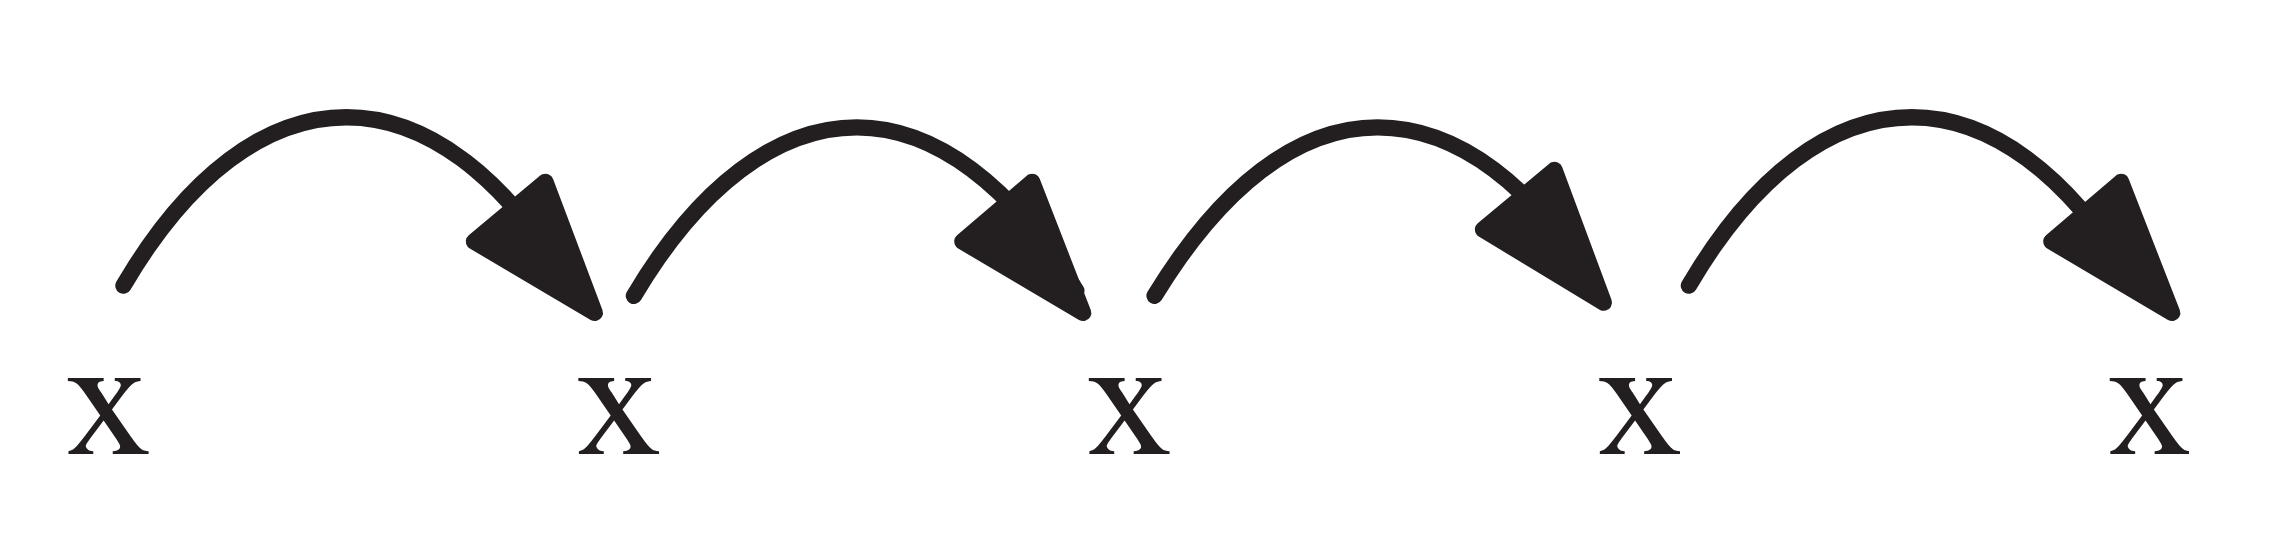
\includegraphics[width=0.5
	\textwidth] {pics/samebranching.png} \caption{\Gls{percabangan-searah} atau \textit{same-branching}} 
\label{fig:samebranching} \end{figure}

\begin{figure}
	\centering 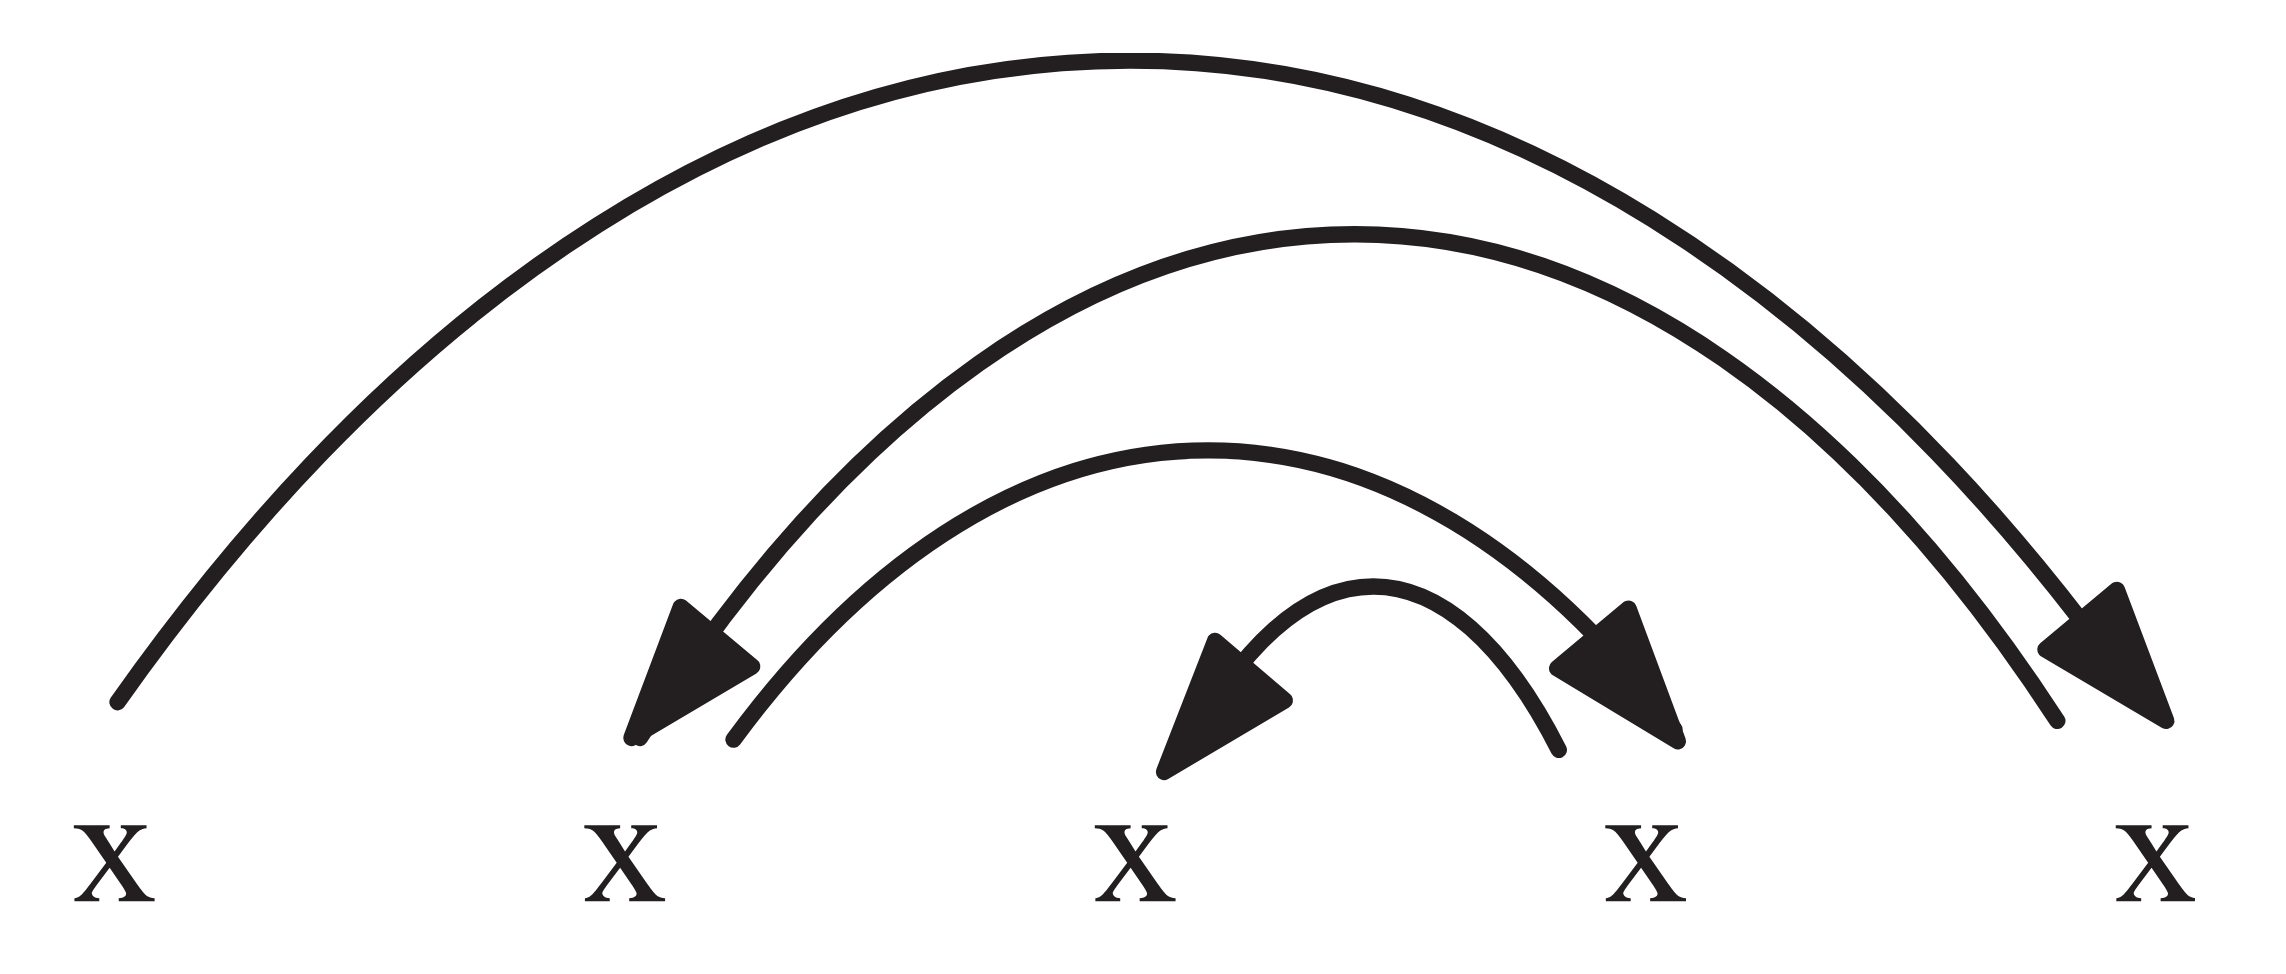
\includegraphics[width=0.5
	\textwidth] {pics/mixedbranching.png} \caption{\Gls{percabangan-beda-arah} atau \textit{mixed-branching}} 
\label{fig:mixedbranching} \end{figure}

Perbandingan percabangan pada \pic~\ref{fig:samebranching} dan \pic~\ref{fig:mixedbranching} mengilustrasikan tautan-tautan yang dibentuk oleh masing-masing tipe percabangan. Percabangan searah atau \textit{same branching} dengan satu relasi yang berkelanjutan tidak mungkin akan secara konsisten terjadi, terutama pada kalimat yang lebih panjang sehingga asumsi ini dipertanyakan oleh \cite{temperley2008dependency} yang menganggap bahwa percabangan searah ini tidak selalu optimal dalam menggambarkan penampilan bahasa. \cite{temperley2008dependency} meneruskan asumsi ini berdasarkan penelitian \cite{dryer1992greenbergian} terhadap 625 bahasa yang mengungkapkan bahwa percabangan searah yang konvensional tidak dapat menggambarkan dengan baik aplikasi tata bahasa pada tuturan nyata dalam studi penampilan bahasa. \cite{dryer1992greenbergian} menggambarkan karakter tata bahasa mengenai hal ini sebagai berikut: frasa yang mengandung banyak konstituen cenderung memiliki percabangan searah, sedangkan arah dependensi frasa yang hanya mengandung satu konstituen ditemukan tidak konsisten. Kajian \cite{dryer1992greenbergian} yang dikutip dalam \cite{gildea2010grammars} memperlihatkan dengan bukti empiris adanya gabungan percabangan searah dan percabangan beda arah (\textit{mixed branching}) untuk menghasilkan keseimbangan antara arah dependensi positif (diawali induk) dan dependensi negatif (diakhiri induk) dalam mendapatkan nilai panjang dependensi terkecil (\pic~\ref{fig:balancedbranching}).

\begin{figure}
	\centering 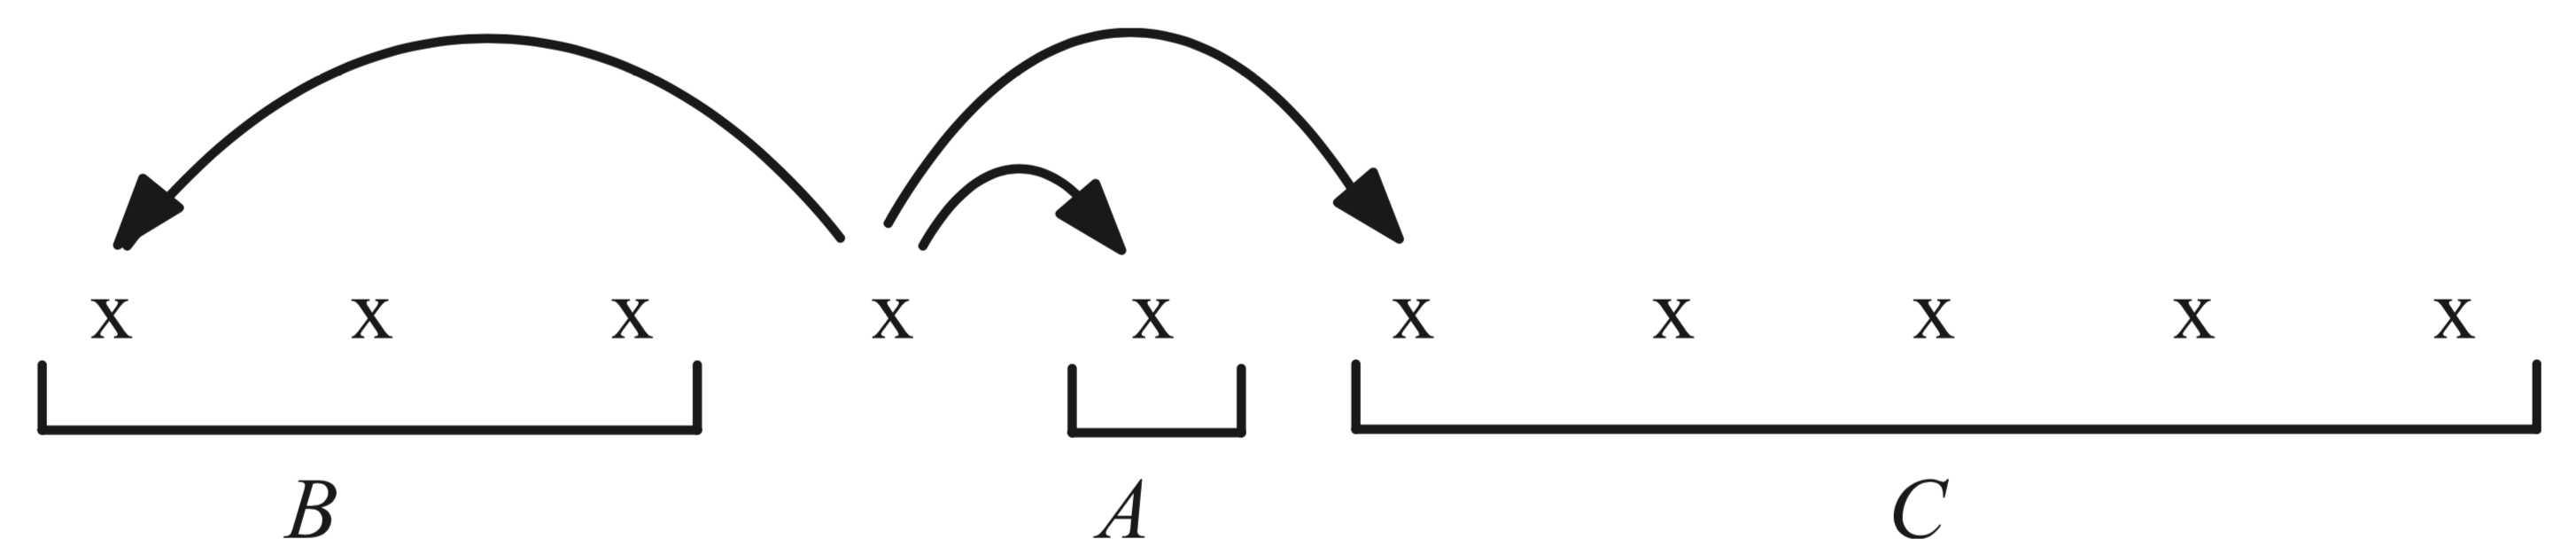
\includegraphics[width=0.8
	\textwidth] {pics/balancedbranching.png} \caption{Keseimbangan direksionalitas induk} 
\label{fig:balancedbranching} \end{figure}

%-----------------------------------------------------------------------------%
\subsection{Faktor-faktor yang mempengaruhi tautan dependensi}
%-----------------------------------------------------------------------------%
Penutur sering menggunakan cara yang berbeda untuk menyampaikan pesan dengan makna yang sama \citep{kroch2001syntactic}. Meskipun penelitian ini hanya menitikberatkan pada variasi sintaktis terkait konsep dependensi, perbedaan karakteristik kalimat ini tidak hanya dalam konteks sintaktis, tetapi juga secara fonetis, fonologis, dan perbedaan leksikal. Hubungan produksi kalimat dipandang dari segi sintaktis dengan memori kerja manusia telah beberapa kali dikaji terutama di ruang lingkup psikolinguistik (\citealp{jay2003psychology, levy2013surprisal}) maupun oleh peneliti di bidang ilmu kognitif (\citealp{futrell2015large, christiansen2016now, liu2017dependency}). Hal ini memperlihatkan bahwa konsep dependensi dapat memberikan kontribusi wawasan tidak hanya dari segi linguistik, namun juga secara multidisipliner.

%-----------------------------------------------------------------------------%
\subsubsection{Kognisi manusia dan produksi kalimat}
%-----------------------------------------------------------------------------%
Panjang dan jarak dependensi antarkonstituen mengindikasikan upaya memori kerja manusia untuk menyimpan secara aktif satu konstituen hingga konstituen lain direalisasikan sehingga maknanya dapat tersampaikan secara utuh (\citealp{hudson2003psychological, liu2008dependency}). Pada penelitian-penelitian terdahulu dalam ruang lingkup ilmu kognitif, memori kerja manusia memiliki batasan (\textit{threshold}) terhadap waktu sehingga proses produksi ataupun pemahaman bahasa tidak bertahan lama dan bersifat sekilas untuk saat itu saja \citep{christiansen2016now}. Oleh karena itu, memori akan bekerja lebih banyak untuk memproduksi ataupun memahami kalimat dengan panjang dan jarak dependensi yang lebih jauh karena kedua indikator tersebut diasumsikan berhubungan linear dengan waktu yang dibutuhkan untuk menyimpan konstituen secara aktif. Dapat dikatakan juga bahwa panjang dan jarak dependensi mengindikasikan tingkat kesulitan sebuah kalimat. 

Melalui pendekatan linguistik kuantitatif, beberapa penelitian telah menunjukkan bukti-bukti kecenderungan bahwa semakin jauh panjang dan jarak dependensi, semakin sulit pemrosesan dan analisis struktur sintaktis semakin sulit (\citealp{gibson1998linguistic, hiranuma1999syntactic, jiang2015effects, temperley2007minimization}). Meskipun penelitian ini tidak menelaah aspek kognisi manusia secara mendalam, temuan penelitian ini dapat dikaitkan dengan temuan penelitian-penelitian tersebut dan memberikan wawasan dari aspek linguistik dalam bahasa Indonesia untuk membentuk hipotesis lanjutan secara lintas bahasa.

%-----------------------------------------------------------------------------%
\subsubsection{Karakter bahasa dan ketatabahasaan}
%-----------------------------------------------------------------------------%
Beberapa penelitian lain yang menggunakan pendekatan linguistik kuantitatif terhadap korpus data teks telah memulai upaya untuk melihat hubungan panjang dan jarak dependensi dengan tipe bahasa (\citealp{hiranuma1999syntactic, eppler2005syntax, liu2012quantitative}), (\citealp{oya2011syntactic, ferrer2014risks, jiang2015effects}), dan tata bahasa (\citealp{liu2008dependency, gildea2010grammars}). Penelitian-penelitian ini belum menunjukkan konsensus terhadap perbedaan mendasar maupun besar dampak dari pengaruh tersebut terhadap dependensinya. Meskipun demikian, beberapa penelitian ini menjadi pondasi untuk memberikan wawasan dan gambaran secara lintas bahasa mengenai kualitas dependensi yang bersifat universal maupun yang menjadi keunikan bahasa masing-masing. \cite{jiang2015effects} menemukan bahwa distribusi jarak dependensi tidak dipengaruhi oleh tipe bahasa. Meskipun demikian, kedua korpus data menunjukkan karakter yang sama, yaitu trend jarak dependensi yang semakin jauh seiring dengan semakin panjangnya kalimat dan rata-rata jarak dependensi dalam bahasa Mandarin lebih tinggi dibandingkan bahasa Inggris. Sebelumnya, \cite{oya2013degree} mendemonstrasikan adanya perbedaan antara jarak dependensi pada teks fiksi dan non-fiksi dalam data bahasa Inggris di mana nilai rata-rata jarak dependensi pada teks fiksi lebih kecil. Namun, \cite{wang2017effects} mengungkapkan bahwa temuan ini dihasilkan tanpa investigasi kemungkinan pengaruh panjang kalimat terhadap jarak dependensi. Hal ini signifikan karena perbedaan rata-rata panjang kalimat antara kedua teks dapat berkontribusi terhadap rata-rata jarak dependensi secara keseluruhan.

Dalam penelitian \cite{hiranuma1999syntactic} dan \cite{liu2009chinese}, teks dialog yang diperuntukkan sebagai ujaran lisan memiliki rata-rata jarak dependensi yang berbeda antara teks imajinatif dan teks informatif. Oleh karena itu, \cite{hiranuma1999syntactic} dan \cite{liu2009chinese} beranggapan bahwa teks yang semakin formal (dalam konteks ini adalah bahasa Inggris ragam tulis) memiliki tingkat sintaktis yang lebih sulit. Sejauh ini belum ada wawasan linguistik yang dapat memberikan informasi terhadap hal tersebut dengan memanfaatkan data bahasa Indonesia. Bahasa Indonesia memiliki konstruksi kalimat umum SVO atau Subyek-Predikat-Obyek, tetapi memiliki aturan urutan kata yang cukup bebas terkait frasa nomina dan frasa verba \citep{irmawati2015dependency}. \cite{kubler2009dependency} menyatakan bahwa analisis sintaktis berdasarkan teori dependensi dapat membantu memahami hubungan antarkonstituen pada bahasa-bahasa dengan aturan urutan kata yang bebas. Munculnya pertanyaan seberapa besar pengaruh kebebasan urutan konstituen terkait pengurangan jarak dependensi ini juga disebabkan oleh pernyataan dalam penelitian \cite{futrell2015large} yang menyebutkan bahwa temuan dalam bahasa Indonesia menunjukkan hasil pengurangan jarak dependensi yang tertinggi dibandingkan 36 bahasa lain yang diteliti.

%-----------------------------------------------------------------------------%
\section{Efisiensi kalimat dari segi dependensi}
%-----------------------------------------------------------------------------%
Hingga abad ke-20, para linguis mengajukan hipotesis pengurangan jarak Euclidean (\textit{Euclidean distance minimization}) untuk jarak antara konstituen-konstituen kalimat yang bertautan secara sintaktis dan fenomena urutan konstituen lainnya (\citealp{i2004euclidean, ferrer2008some}). Hal ini berkaitan dengan usaha penutur dalam menghasilkan kalimat yang efisien sesuai dengan penelitian yang dilakukan \cite{gildea2015human}. \cite{gildea2015human} menguji hipotesis bahwa penutur cenderung menyusun konstituen dalam kalimat untuk menyampaikan informasi secara efisien dan menemukan bahwa semua bahasa yang menjadi obyek penelitiannya memiliki urutan konstituen yang lebih mudah diproses dan dimengerti. Dalam penelitian tersebut, Gildea dan Jaeger menarik korelasi antara kesaratan informasi dan jarak dependensi dengan menitikberatkan pada urutan konstituen dalam kalimat. Saat ini, istilah \textit{Euclidean distance minimization} digantikan dengan istilah pengurangan memori dalam jaringan atau \textit{online memory minimization} karena para peneliti bahasa melihat korelasi yang signifikan antara pengurangan jarak antarkonstituen dalam sebuah kalimat dengan kemudahan proses memori kerja \citep{ferrer2015placement}. Rata-rata jarak dependensi menjadi ukuran penting dalam memprediksikan tingkat kesulitan atau kemudahan sintaktis ini \citep{hudson1995measuring}. Hipotesis bahwa penutur cenderung mengurangi atau meminimalkan jarak dependensi kemungkinan disebabkan oleh keterbatasan memori kerja manusia yang beradaptasi terhadap faktor tata bahasa (\citealp{i2004euclidean, ferrer2016non, buch2006discontinuous, liu2008dependency, gildea2010grammars, futrell2015large}).

%-----------------------------------------------------------------------------%
\subsection{Kaitan pengurangan panjang dan jarak dependensi dengan proses memori kerja}
%-----------------------------------------------------------------------------%
Beberapa studi berbasis empiris telah dilakukan untuk mengeksplorasi kesulitan pemahaman sebuah bahasa, terutama dalam ranah psikolinguistik dan linguistik kognitif \citep{jay2003psychology}. Pendekatan kuantitatif pada ilmu linguistik dalam penelitian seperti ini terus berkembang hingga saat ini dan penggunaan pendekatan-pendekatan tersebut memberikan kontribusi terhadap akurasi metode linguistik kuantitatif yang dikembangkan. \cite{yngve1960model} merupakan salah satu linguis yang mengajukan konsep jumlah 'simbol' maksimum yang dapat disimpan dalam memori kerja saat mengkonstruksi sebuah kalimat. Hipotesis Kedalaman atau \textit{Depth Hypothesis} yang dikembangkan \cite{yngve1960model} diterjemahkan sebagai konsep untuk menganalisis kesulitan pemahaman sebuah kalimat. Isi hipotesis ini adalah bahwa (a) meskipun semua bahasa memiliki tata bahasa, (b) sebuah kalimat memiliki kedalaman yang tidak melebihi angka tertentu (c) sejumlah atau mendekati jumlah yang merepresentasikan memori kerja cepat dan (d) tata bahasa dari semua bahasa tersebut akan menyertakan metode-metode untuk membatasi konstruksi regresif sehingga kalimat tidak akan melewati batas kedalaman (\citealp{yngve1960model, yngve1996grammar}). Dari hipotesis ini dapat diambil kesimpulan bahwa meskipun tata bahasa memungkinkan adanya kalimat-kalimat yang lebih dalam secara teoretis, dalam prakteknya kedalaman tersebut tidak dapat melewati batas tertentu yang setara dengan kapasitas memori kerja manusia (\citealp{miller1956magical,cowan2001metatheory}). Dengan hipotesis ini, \cite{yngve1960model} mencoba membangun indikator universal untuk kesulitan pemahaman sebuah kalimat. 

\cite{miller1963finitary} mengajukan indikator kompleksitas sintaktis berdasarkan rasio dari simpai akhir dan simpai bukan akhir pada bank pohon struktur sintaktis sebuah kalimat. Pendekatan ini dilanjutkan oleh \cite{frazier1985syntactic} yang menggunakan penghitungan dengan menyesuaikan konteks bahasa lokal untuk mengganti penghitungan global yang bersifat lintas bahasa milik \cite{miller1963finitary} agar indikator tersebut lebih sensitif dan kontekstual. \cite{hawkins1994performance} kemudian muncul dengan asumsi mengenai keterkaitan antara tata bahasa dan urutan kata. Untuk mengukur dan memperkirakan kesulitan sintaktis, Hawkins mengembangkan prinsip Konstituen Terdekat Awal atau \textit{Early Immediate Constituents} (EIC) yang menyatakan bahwa manusia cenderung memilih urutan linear yang memaksimalkan rasio Konstituen Terdekat (IC) terhadap non-IC dalam jangkauan pemahaman ujaran. \cite{hawkins2004efficiency} memperbaharui EIC menjadi Meminimalkan Jangkauan atau \textit{Minimize Domain} (MiD) dengan memanfaatkan teori dependensi. Prinsip ini menyatakan bahwa manusia cenderung meminimalkan deret unit linguistik yang memiliki relasi semantis dan/atau meminimalkan proses dependensi yang terlibat \citep{hawkins2004efficiency}. Prinsip ini secara langsung memperlihatkan keterkaitan antara urutan linear konstituen linear dengan pengolahan bahasa yang dilakukan dalam memori kerja manusia.

Hipotesis yang muncul dari penelitian-penelitian tersebut menggambarkan ketertarikan dunia linguistik atas indikator kompleksitas kalimat yang melibatkan hubungan antara urutan linear konstituen, kesulitan sintaktis serta bagaimana dependensi antarunit linguistik berperan di dalam konteks indikator kompleksitas tersebut. Penekanan dependensi dalam area penelitian ini adalah jika struktur kognitif manusia berbentuk seperti jejaring \citep{hudson2007language}, analisis terhadap jejaring dependensi sintaktis juga merupakan langkah penting menuju pemetaan jejaring kognitif konseptual yang secara langsung menggambarkan kerja kognisi manusia \citep{liu2008dependency}. \cite{liu2008dependency} menyimpulkan bahwa dibandingkan dengan struktur frasa, keterkaitan struktur dependensi dengan struktur kognitif dan jejaring bahasa, memiliki hubungan yang lebih dekat. Terdapat kesamaan dalam prinsip-prinsip dari berbagai penelitian tersebut, yaitu indikasi bahwa konstituen-konstituen yang memiliki relasi semantik cenderung akan berdekatan dalam kalimat. 

\cite{liu2017dependency} mengembangkan proposal indikator yang menggunakan jarak dependensi menjadi hipotesis \textbf{Pengurangan Jarak Dependensi} atau \textit{Dependency Distance Minimization} (yang selanjutnya akan disingkat menjadi DDM). Sebagai contoh, istilah 'jarak' sering digunakan jika seseorang bergerak menuju sebuah tempat hingga orang tersebut berhenti. Dalam proses produksi dan pemahaman bahasa, 'jarak' dependensi baru akan dapat terukur apabila dependensi kedua konstituen telah terbentuk (konstituen kedua sudah diujarkan, dibaca, ditulis, atau didengar). \cite{liu2017dependency} berargumen bahwa 'panjang' merefleksikan ukuran dengan karakteristik statis dari sebuah entitas dan 'jarak' lebih menggambarkan proses dinamis sehingga dalam konteks dependensi sebuah kalimat, para peneliti tersebut beranggapan istilah 'jarak' lebih tepat digunakan. Untuk mendapatkan gambaran DDM, Liu (\citealp{liu2008dependency, liu2017dependency}) menjabarkan rumus untuk menghitung \textbf{Rata-rata Jarak Dependensi}. \cite{hudson2010introduction} dan \cite{i2004euclidean} menggunakan pendekatan yang kurang lebih sama untuk menghitung MDD dalam sebuah kalimat. Dalam studinya, \cite{i2004patterns} melakukan kajian untuk memperlihatkan bahwa jejaring sintaksis merupakan contoh 'dunia-dunia kecil' yang berarti angka rata-rata dari tautan dalam simpai ditemukan sangat kecil. Hipotesis utama DDM dijabarkan Liu (\citealp{liu2008dependency, liu2017dependency}) sebagai berikut:

\begin{itemize}
\item Manusia cenderung memilih urutan konstituen yang dapat mengurangi rata-rata jarak dependensi.
\item Terdapat batasan rata-rata jarak dependensi pada hampir semua kalimat dalam bahasa manusia.
\item Tata bahasa dan kognisi manusia bekerja sama untuk menekan jarak dependensi agar berada di dalam batasan tersebut.
\end{itemize}

Dalam penelitian lintas bahasa berskala besar lain, \cite{futrell2015large} menggunakan hipotesis \textbf{Pengurangan Panjang Dependensi} atau \textit{Dependency Length Minimization} (yang selanjutkan akan disingkat menjadi DLM). Penelitian lintas bahas ini memanfaatkan korpus data sebanyak 37 bahasa, termasuk bahasa Indonesia. Hipotesis ini sebelumnya muncul dalam penelitian Temperley dan Gildea (\citealp{temperley2007minimization, temperley2008dependency, gildea2010grammars}). \cite{gildea2010grammars} menggunakan istilah 'panjang' dalam DLM karena menitikberatkan pada kompleksitas keseluruhan kalimat. Penghitungan yang digunakan untuk melihat indikasi DLM didapatkan dengan menjumlahkan keseluruhan jarak tautan-tautan dependensi dalam sebuah kalimat seperti yang terlihat pada Gambar 1.1 di Bab 1. \cite{liu2017dependency} dan \cite{i2004euclidean} beranggapan bahwa pendekatan ini cukup sensitif terhadap panjang kalimat atau kalimat sehingga perbedaan rata-rata yang muncul kurang bisa mewakili kesulitan sintaktis karena ada kecenderungan bahwa kalimat yang semakin panjang akan menghasilkan angka lebih besar. Hipotesis utama dari DLM dijabarkan oleh \cite{gildea2010grammars} serta \cite{futrell2015large} sebagai prinsip bahasa yang telah banyak diakui mengenai preferensi penutur untuk mendekatkan konstituen-konstituen yang memiliki relasi semantis dalam sebuah kalimat.

%-----------------------------------------------------------------------------%
\subsection{Perubahan valensi akar verbal}
%-----------------------------------------------------------------------------%
Penjabaran konsep dependensi juga mencakup seberapa kuat sebuah konstituen mengikat konstituen lain dalam kalimat. Dalam teori dependensi \citep{tesniere1959elements} dan \textit{Word Grammar} \citep{hudson2007language}, kemampuan sebuah induk (sebagai contoh: verba) menarik konstituen di sekitarnya (sebagai contoh: aktor pelaku yang umumnya adalah nomina) disebut dengan \textbf{valensi}. Sebagai ilustrasi, agar penerapan konstituen \textit{memandangi} dalam kalimat menjadi gramatikal, konstituen tersebut (yang memiliki fungsi sebagai proses) menuntut keterlibatan dua konstituen lain seperti pada kalimat: $Budi_1$ $memandangi$ $lukisan_2$. Verba \textit{memandangi} mengalokasikan fungsi \textit{Budi} sebagai \textit{yang memandangi} (aktor pelaku atau \textit{agent}) pada posisi pertama, dan \textit{lukisan} sebagai \textit{yang dipandangi} (obyek penderita atau \textit{patient}) \citep{welke2002deutsche}. Kebutuhan fungsional verba tersebut menentukan kategori dan posisi yang harus diisi agar sebuah kalimat menjadi gramatikal. Tidak hanya pelengkap, verba juga dapat berkombinasi dengan keterangan (\textit{adjunct}) seperti pada kalimat: $Budi_1$ $memandangi$ $lukisan_2$ $di$ $museum_3$. Pelengkap juga dapat bersifat tidak wajib seperti pada contoh $dia_1$ $membaca$ $buku_2$ dan $dia_1$ $membaca$. Konstituen \textit{buku} merupakan obyek penderita langsung yang tidak wajib muncul agar pendengar memahami proses \textit{membaca}. 

Hingga saat ini, belum ada pendekatan linguistik kuantitatif ataupun perangkat komputasional dan inventori leksikon valensi untuk bahasa Indonesia. Oleh karena itu, analisis valensi dalam penelitian ini dilakukan secara manual atau bersifat kualitatif dengan menggunakan referensi dari anotasi yang ada. Analisis valensi dalam penelitian ini mengambil obyek berupa akar verbal pada simpai pusat karena diduga merupakan bentuk rangka valensi yang paling umum. Perlu ditekankan bahwa analisis valensi ini tidak ditujukan untuk mengidentifikasi kalimat yang bersifat gramatikal dan tidak gramatikal, namun menitikberatkan pada fenomena linguistik yang muncul dalam tuturan nyata sesuai dengan korpus data yang dikumpulkan. Meskipun kemunculan akar verbal pada simpai pusat diduga memiliki frekuensi tertinggi, beberapa nomina dan adjektiva juga dapat muncul pada simpai pusat dan memiliki valensi tertentu (\citealp{vreznivckova2003czech, hajic2003pdt}).

%-----------------------------------------------------------------------------%
\section{Dependensi dan urutan kata dalam bahasa Indonesia}
%-----------------------------------------------------------------------------%
Dalam tipologi berbagai penelitian bahasa, ternyata terdapat kecenderungan kuat dalam banyak bahasa untuk mengatur tata bahasanya agar menghasilkan kalimat dengan pemrosesan ranah yang minimal \citep{hawkins2001second}. Sebagai contoh, \cite{hiranuma1999syntactic} menemukan bahwa aturan pilihan konstituen terikat (\textit{optionality of dependents}) dalam bahasa Jepang memberikan kompensasi terhadap letak induk yang selalu berada di akhir dalam urutan kata (\textit{head-final}). Tanpa kompensasi ini, rata-rata jarak dependensi akan menjadi jauh lebih besar dibandingkan dengan bahasa Inggris yang letak induknya bervariasi (\textit{mixed-order}). Hasil dari pilihan ini adalah konstituen terikat per induk dalam bahasa Jepang lebih sedikit dibandingkan dengan bahasa Inggris sehingga rata-rata jarak dependensi pada data yang diteliti Hiranuma antara bahasa Jepang dan Inggris hampir sama. Di sisi lain, terdapat juga bukti empiris bahwa beberapa bahasa mentolerir kadar kesulitan tersebut seperti pada perbandingan jarak dependensi antara bahasa Inggris dan Jerman yang dilakukan oleh \cite{eppler2005syntax}. \cite{eppler2005syntax} menemukan bahwa jarak dependensi dalam bahasa Jerman yang lebih tinggi mungkin dikarenakan tekanan untuk meminimalkan jarak dependensi bertentangan dengan tekanan fungsional lainnya.

Tantangan utama dalam bahasa Indonesia adalah bahwa batas antara kelas kata yang satu dengan yang lain tidak sejelas yang diharapkan (\citealp{kridalaksana2002struktur, achmad2013linguistik}). Namun, \cite{kridalaksana2002struktur} juga mengungkapkan bahwa dalam menentukan kelas kata dalam bahasa Indonesia, perilaku sintaktis dapat dijadikan ciri dasar. Sesuai saran \cite{robins1985linguistics}, paradigma morfologis juga mendukung penentuan kelas kata ini. Salah satu perilaku sintaktis yang disebut \cite{kridalaksana2002struktur} adalah bagaimana sebuah konstituen memiliki tautan dependensi dengan konstituen lain dalam konstruksi kalimat. \cite{demena2008bahasa} juga menyebutkan bahwa verba tidak hanya ditempatkan sebagai dasar untuk menjelaskan proses dalam bahasa Indonesia, tetapi juga menjadi dasar dalam mayoritas pembentukan kalimat \citep{kridalaksana1999deskriptif}.

%-----------------------------------------------------------------------------%
\subsection{Urutan kata dalam tata bahasa Indonesia}
%-----------------------------------------------------------------------------%
\cite{wasow2002postverbal} beranggapan bahwa karena perbedaan makna antara tiap bentuk (\textit{alternant}) dapat diabaikan, preferensi terhadap satu kalimat dibandingkan yang lain didorong oleh pertimbangan pengolahan dalam memori kerja sebagai motivasi utama. \cite{wasow2002postverbal} mengajukan Prinsip Bobot Akhir atau \textit{Principle of End Weight} (PEW) sebagai penjelasan tendensi tersebut. PEW menyatakan bahwa saat dihadapkan dengan pilihan, manusia cenderung menempatkan konstituen dengan bobot terberat seakhir mungkin dalam sebuah kalimat. \cite{rosenbach2005animacy} meneliti peran bobot konstituen atau frasa dalam alternasi genitif seperti pada contoh \textit{the boy's face} dan \textit{the face of the boy}. Dalam PEW, 'pemilik' memiliki bobot lebih tinggi oleh karena itu bentuk kalimat yang kedua seharusnya lebih banyak dipilih penutur karena menempatkan konstituen dengan bobot lebih besar lebih dekat ke akhir kalimat. \cite{francis2010grammatical} dan \cite{rosenbach2005animacy} juga melihat efek bobot tersebut dalam ranah produksi (penutur) maupun pemahaman (pendengar). \cite{francis2010grammatical} melihat kecenderungan pemilihan bentuk ekstraposisi saat klausa relatif memiliki bobot lebih seperti pada contoh \textit{three people who were from Chicago arrived here yesterday} dan \textit{three people arrived here yesterday who were from Chicago}.

Dalam bahasa Indonesia, terdapat gambaran umum mengenai urutan kata sehingga sebuah kalimat menjadi gramatikal. Seperti yang dibahas dalam \textit{Indonesian Reference Grammar} \citep{sneddon2010indonesian}, beberapa urutan kata untuk frasa nomina adalah:
\begin{itemize}
\item Nomina yang memodifikasi langsung mengikuti induknya
\item Pemilik mengikuti adjektiva
\item Nomina atributif dalam frasa nomina perbuatan mengikuti adjektiva
\item Klausa relatif mengikuti nomina yang memodifikasi, adjektiva, dan pemilik
\item Demonstrativa mengikuti konstituen-konstituen lain dalam frasa
\end{itemize}

\cite{sneddon2010indonesian} juga mengungkapkan bahwa beberapa pertukaran posisi urutan kata tidak mengubah maknanya seperti \textit{sudah harus} dan \textit{harus sudah}. Urutan kata yang paling umum dalam klausa adalah subyek + predikat dan subyek + predikat + obyek dalam klausa verba transitif. Obyek primer akan menempati posisi lebih depan dibandingkan obyek sekunder. Secara umum, klausa pasif memiliki dua tipe, (i) bentuk subyek + verba + pelaku dan (ii) subyek + pelaku + verba \citep{sneddon2010indonesian}. Meskipun keterangan cenderung menempati posisi tertentu di dalam klausa, pada kenyataannya urutan ini jauh lebih bebas dibandingkan dengan komponen nukleus. Dilihat secara gramatikal, perubahan urutan kata dilakukan untuk memfokuskan perhatian terhadap komponen tertentu \citep{sneddon2010indonesian}, namun dalam penelitian penampilan bahasa, hal ini tidak selalu menggambarkan konsep gramatikal yang dituju.

%-----------------------------------------------------------------------------%
\subsection{Simpai pusat dalam bahasa Indonesia}
%-----------------------------------------------------------------------------%
Hingga saat ini, belum ada teori atau penelitian terkait teori dependensi dan simpai pusat dalam bahasa Indonesia, namun teori-teori terkait tata bahasa yang ada dapat menjadi referensi awal untuk melihat perilaku simpai pusat dalam bahasa Indonesia. Berkaitan dengan kebebasan urutan kata dalam bahasa Indonesia (terutama posisi keterangan), simpai pusat pada sebuah kalimat menempati posisi yang tidak tentu seperti pada contoh perbedaan posisi klausa utama pada \textit{kalau pulang, tolong belikan nasi bungkus} dan \textit{tolong belikan nasi bungkus kalau pulang} \citep{sneddon2010indonesian}. Perbedaan posisi klausa utama pada kedua kalimat tersebut berkaitan dengan perbedaan posisi simpai pusat serta keterlibatan jeda (\textit{pause}) dalam kalimat yang diwakilkan oleh tanda baca koma (,). Secara lisan maupun tulisan, jeda ini berpengaruh terhadap proses konstruksi kalimat sehingga patut diperhitungkan juga dalam mengkonstruksikan kalimat dan menganalisis struktur sintaktis. 
Bahasa Indonesia memiliki beragam klausa tanpa verba yang banyak ditemukan dalam pemakaian sehari-hari baik secara lisan maupun tulisan \citep{sneddon2010indonesian} seperti klausa nomina, klausa adjektiva, klausa preposisional, dan penggunaan kopula. Teori dependensi dapat digunakan untuk menganalisis karena simpai pusat tidak selalu melibatkan verba \citep{tesniere1959elements}. Dalam kasus-kasus seperti itu, identifikasi induk dilakukan dengan melihat tautan terbanyak \citep{tesniere1959elements} dan mempertimbangkan jenis klausa itu sendiri \citep{sneddon2010indonesian}.
%-----------------------------------------------------------------------------%
\chapter{\babTiga} \label{chap:metode_penelitian}
%-----------------------------------------------------------------------------%

%-----------------------------------------------------------------------------%
\section{Metode penelitian}
%-----------------------------------------------------------------------------%
Penelitian tesis ini memanfaatkan dasar teori dependensi yang menjadi ancangan untuk kerangka teori dan metode penelitian. Semua temuan yang dipaparkan dalam penelitian ini didasarkan pada korpus data yang terkumpul dan keterkaitannya terhadap teori yang dibahas. Korpus bahasa Indonesia ragam tulis dan lisan diolah dan dianalisis dengan ancangan yang memadukan pendekatan analisis linguistik kuantitatif dan kualitatif. Langkah-langkah dalam penelitian yang dijelaskan dalam bab ini melibatkan (a) penjelasan mengenai sumber data dan pengumpulan data menjadi dua korpus utama, (b) pengolahan data yang mencakup tahap penguraian kalimat berdasarkan dependensi, anotasi Panjang Dependensi (DL) dan Rata-rata Jarak Dependensi (MDD) terhadap semua kalimat di dalam korpus, seleksi dan klasifikasi data tersebut untuk keperluan analisis, serta (c) teknik-teknik analisis data untuk pemaparan temuan terkait Pengurangan Panjang Dependensi (DLM) dan Pengurangan Jarak Dependensi (DDM) antarkonstituen secara kuantitatif dan analisis kualitatif untuk melihat struktur kalimat-kalimat berdasarkan temuan tersebut, pengaruh panjang kalimat terhadap struktur dependensi, serta perubahan valensi akar verbal.

%-----------------------------------------------------------------------------%
\section{Sumber data}
%-----------------------------------------------------------------------------%

Merujuk pada pokok permasalahan penelitian ini yang menitikberatkan pada efisiensi kalimat dipandang dari segi dependensi, teks yang digunakan dalam kedua korpus data difokuskan kepada satu aliran, yaitu teks informatif. Pemilihan satu aliran teks ini didasarkan pada pertimbangan untuk menyeimbangkan kuantitas dan kualitas data sehingga analisis tidak melebar akibat perbedaan aliran teks. Sebelumnya, \cite{miller2011critical} melihat adanya perbedaan kerumitan sintaktis dalam teks informatif itu sendiri, seperti halnya media cetak formal akan lebih kompleks dibandingkan dengan artikel tabloid. Hal ini menunjukkan bahwa data penelitian linguistik terkait dependensi dapat fokus kepada salah satu aliran teks (informatif atau imajinatif) dan tetap mendapatkan gambaran keragaman pola yang ada di dalamnya. Penelitian-penelitian terdahulu yang menggunakan dasar teori dependensi dalam konteks bahasa Indonesia menggunakan korpus data hanya mencakup data ragam tulis dari berbagai jenis media seperti jurnalistik, blog, artkel penelitian, dan media sosial sehingga variabel aliran teks tidak menjadi pertimbangan. Pemilahan korpus data tersebut dilakukan dengan dasar keragaman serta kuantitas data untuk mendapatkan gambaran luas pada bahasa Indonesia ragam tulis (\citealp{kamayani2011dependency, green2012indonesian, irmawati2015dependency, futrell2015large}). 

\cite{wang2017effects} menemukan bahwa teks imajinatif seperti novel, cerita pendek, dan karya literatur lainnya cenderung memiliki jarak dependensi yang lebih jauh dibandingkan dengan teks informatif. Sehingga, untuk melihat penekanan dalam efisiensi kalimat dan kaitanya dengan struktur dependensi, aliran teks lebih tepat untuk digunakan dalam penelitian ini. Saat ini, teks informatif tidak hanya hadir dalam media jurnalistik formal tetapi juga dalam blog dan sosial media dengan bahasa tidak baku atau sehari-hari. Namun, sumber daya teknologi untuk mengolah data bahasa non-formal tersebut masih sangat kurang memadai sehingga tidak memungkinkan peneliti untuk melakukan penelitian skala besar \citep{green2012indonesian}. Oleh karena itu, penelitian tesis ini memfokuskan pada data jurnalistik bahasa Indonesia mencakup ragam tulis dan lisan karena memiliki kaidah yang cukup formal untuk dapat dipadankan dibandingkan dengan aliran fiksi yang kaidahnya terlalu bebas. 

%-----------------------------------------------------------------------------%
\subsection{Data jurnalistik ragam tulis}
%-----------------------------------------------------------------------------%
Salah satu cara dalam pengumpulan data untuk korpus jurnalistik ragam tulis ini bekerjasama dengan perusahaan Indonesia bernama Dattabot yang salah satu ruang lingkup kerjanya bergerak di bidang media monitoring. Korpus ragam tulis ini mencakup dokumentasi data jurnalistik dari berbagai media cetak (\pic~\ref{fig:contoh-tulis-mentah}) dengan kurun waktu publikasi dari tahun 2008 hingga 2018. Teks dalam korpus data ragam tulis ini mencakup total 19.530 kalimat yang secara keseluruhan mengandung total 270.409 konstituen. Pemilahan data teks untuk dimasukkan ke dalam korpus penelitian tesis ini dilakukan secara acak dari korpus yang lebih besar milik Dattabot dengan kriteria sebagai berikut:

\begin{itemize}
	\item Jenis media cetak mencakup artikel daring (\textit{online}), surat kabar, majalah, dan tabloid
	\item Topik mencakup berita kriminal, politik, bencana, lalu lintas, hiburan/budaya, pendidikan, teknologi, olahraga, bisnis/keuangan, dan umum
\end{itemize}

\begin{figure}
	\centering 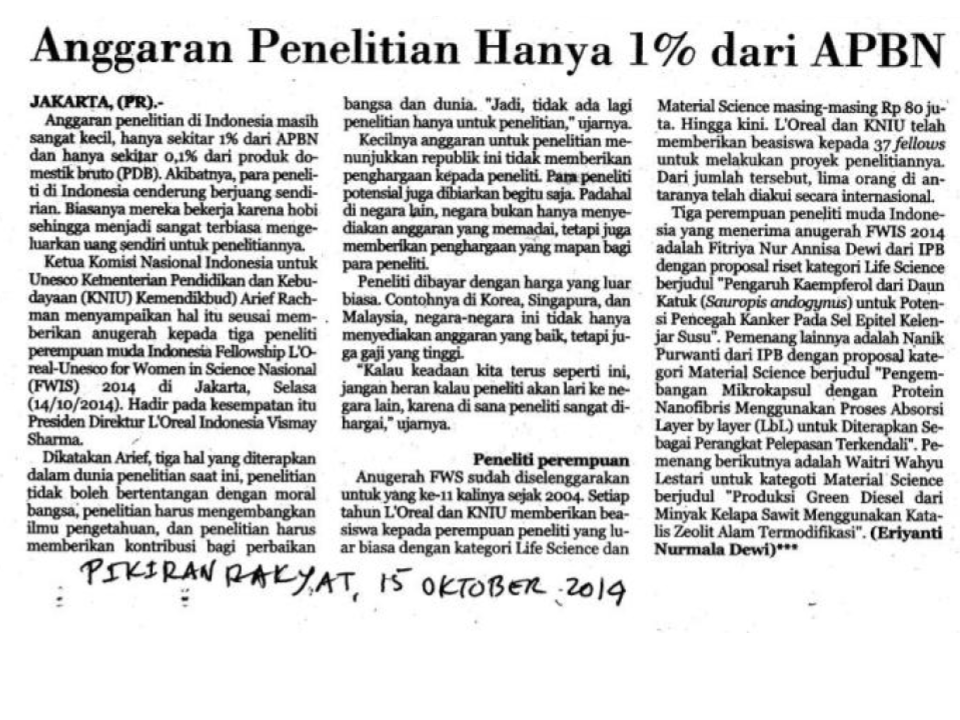
\includegraphics[width=1
	\textwidth] {pics/contoh-tulis-mentah.png} \caption{Contoh data mentah ragam tulis} 
\label{fig:contoh-tulis-mentah} 
\end{figure}

%-----------------------------------------------------------------------------%
\subsection{Data jurnalistik ragam lisan}
%-----------------------------------------------------------------------------%
Penelitian ini memanfaatkan juga dokumentasi data jurnalistik berupa rekaman laporan berita dan wawancara dengan narasumber dengan waktu rekaman dari tahun 2010 hingga 2018. Pengumpulan data ragam lisan dilakukan dengan bantuan para jurnalis dari berbagai media dan daerah di Indonesia yang mengunggah rekaman secara \textit{online} dan video jurnalistik \textit{online} yang ditranskripsi. Teks dalam korpus data ragam lisan ini mencakup total 10.219 kalimat yang secara keseluruhan mengandung total 108.208 konstituen. Pemilahan data ragam lisan untuk dimasukkan ke dalam korpus berdasarkan kriteria sebagai berikut:

\begin{itemize}
	\item Jenis media untuk para jurnalis mencakup televisi, radio, surat kabar, majalah dan tabloid
	\item Topik berita kriminal, politik, bencana, lalu lintas, hiburan/budaya, pendidikan, teknologi, olahraga, bisnis/keuangan, dan umum
	\item Isi rekaman berupa laporan berita atau wawancara dengan narasumber
\end{itemize}

Pengumpulan korpus data ragam lisan memakan waktu lebih lama dibandingkan korpus data ragam tulis karena harus melalui beberapa tahap sebelum dapat diolah pada langkah penelitian selanjutnya. Tahap pertama yang dilakukan untuk persiapan data ragam ilisan adalah proses verifikasi terhadap isi rekaman untuk memastikan tidak lebih dari 10\% isi rekaman yang bersifat pembacaan naskah. Proses persiapan awal ini menjadi perhatian penting untuk mendapatkan kualitas data korpus yang mendekati murni lisan. Tahap kedua dalam persiapan korpus data jurnalistik ragam lisan seperti pada \pic~\ref{fig:contoh-transkripsi-lisan} adalah transkripsi rekaman audio menjadi teks tulisan dengan metode komputasional yang kemudian diverifikasi secara manual agar dapat dianalisis dengan metode serupa seperti yang dilakukan terhadap data ragam tulis. 

\begin{figure}
	\centering 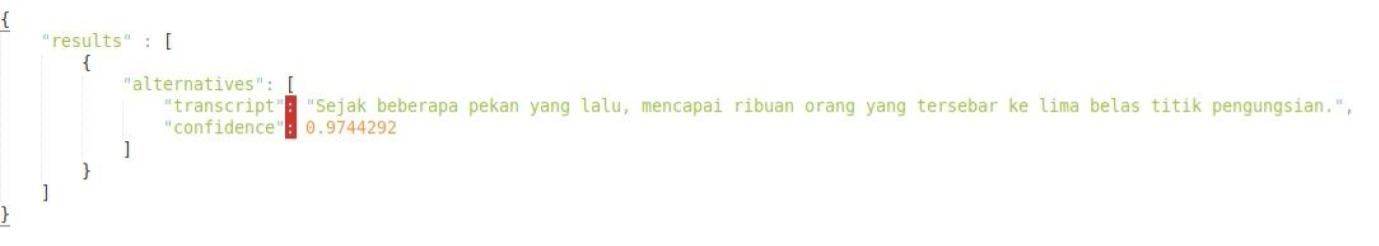
\includegraphics[width=1
	\textwidth] {pics/contoh-transkripsi-lisan.png} 
	\caption{Contoh hasil transkripsi data ragam lisan} 
	\label{fig:contoh-transkripsi-lisan} 
\end{figure}

Tahap terakhir dari persiapan korpus data ragam lisan adalah eliminasi kalimat-kalimat yang tidak selesai agar tidak mengganggu proses pengolahan data. Hal ini dilakukan karena keterbatasan metode penguraian kalimat yang masih belum bisa menguraikan kalimat yang tidak selesai. Dengan proses ini maka seluruh teks dalam data ragam lisan berisi kalimat utuh dan lebih dapat disandingkan dengan data ragam tulis dalam analisisnya.

%-----------------------------------------------------------------------------%
\section{Pengolahan data}
%-----------------------------------------------------------------------------%

Penelitian ini merupakan penelitian yang bersifat sinkronis terhadap data jurnalistik termutakhir baik untuk ragam tulis maupun lisan. Tujuan utama penelitian ini adalah mengeksplorasi adanya indikasi efisiensi kalimat dan memaparkan strategi-strategi pembentukan struktur kalimat pada kedua ragam. Oleh karena itu, penelitian ini tidak memfokuskan pada leksikon dan konteksnya seperti pada pendekatan linguistik korpus secara umum. Variasi topik dalam pengumpulan data dilakukan untuk memastikan keragaman dalam satu aliran teks tersebut terjaga agar memberikan gambaran dependensi yang tidak terkait topik. Hal ini juga dilakukan untuk mempermudah proses pengolahan data yang mencakup beberapa tahap komputasi.

%-----------------------------------------------------------------------------%
\subsection{Perangkat pengolahan data}
%-----------------------------------------------------------------------------%
Data jurnalistik ragam tulis yang diterima dari hasil kerja sama dengan perusahaan media monitoring Dattabot berbentuk teks elektronik hasil pemindaian media cetak dengan pendekatan komputasional \textit{Optical Character Recognition} (OCR). Sedangkan, data jurnalistik ragam lisan berupa rekaman audio yang diolah terlebih dahulu dalam salah satu tahap persiapan data menggunakan metode komputasional dengan bantuan Google Speech API dan diverifikasi kembali secara manual. Tahap 
 memanfaatkan UDPipe \citep{udpipe2017} yang merupakan sebuah kerangka kerja yang dapat dilatih ulang untuk pengkategorian konstituen kalimat (\textit{token}), penguraian lemma, dan penguraian kalimat. Kerangka kerja UDPipe digunakan sebagai langkah penguraian kalimat komputasional dan dijalankan sebagai paket CRAN pihak ketiga UDPipe versi 0.5 \cite{udpipe2017manual} pada bahasa pemrograman R (versi 3.3.3) \citep{r2017project}. 

Umumnya, kerangka kerja atau pendekatan penguraian kalimat dalam ranah linguistik komputasional memanfaatkan teori konstituensi sebagai dasar teori dan pengembangannya sehingga menghasilkan uraian kalimat berdasarkan struktur frasanya. Kerangka kerja penguraian kalimat UDPipe menggunakan dasar diagram pohon dependensi Universal Dependencies 2.0 \citep{nivre2017universal} dengan memadukan lemma dan fitur morfologis lainnya dari kerangka kerja MorphInd yang kontekstual terhadap data bahasa Indonesia \citep{larasati2011indonesian}. Kerangka kerja penguraian kalimat berdasarkan dependensi saat ini masih terus dikembangkan secara intensif sehingga masih memiliki kekurangan dalam aspek menangani keambiguitasan makna konstituen, bentuk bahasa informal, dan masalah ujaran nyata lainnya. Kekurangan ini menuntut tahapan verifikasi manual untuk memastikan kualitas data. Meskipun begitu, hasil uji model terhadap bahasa Indonesia memiliki akurasi 74,3\%-80,6\% \citep{udpipe2017}. Setelah melalui proses penguraian kalimat, seluruh tahapan-tahapan berikutnya yang mencakup anotasi nilai DL dan MDD, seleksi dan klasifikasi data, analisis teks, pemaparan pola DL dan MDD, serta uji signifikansi memanfaatkan bahasa pemrograman R (versi 3.3.3) \citep{r2017project} dan Python (versi 3.6.3) (Python Core Team, 2017).

%-----------------------------------------------------------------------------%
\subsection{Penguraian kalimat}
%-----------------------------------------------------------------------------%
Prinsip mendasar dalam menguraikan tautan dependensi secara sintaktis dapat dilihat pada \pic~\ref{fig:tautandependensi} (\citealp{tesniere1959elements, hudson1984word, liu2008dependency, liu2017dependency}). Secara mendasar, tautan dependensi ini merupakan tautan yang bersifat asimetris dan biner antara dua unit linguistik \citep{tesniere1959elements}. Tautan dependensi yang terbentuk antara dua unit linguistik atau dua konstituen tersebut direpresentasikan oleh panah yang mengarah dari pengendali yang merupakan akar atau induk ke arah subordinatnya yang merupakan konstituen terikat\footnote{Apabila konstituen terikat mengikat konstituen terikat lain, maka subordinat dapat merupakan induk.}. Tautan dependensi yang terbentuk berbeda-beda tergantung dari relasi antara kedua konstituen, sehingga memerlukan anotasi tipe dependensi agar dapat diidentifikasi. Pada \pic~\ref{fig:tautandependensi}, tipe dependensi ini dianotasikan di atas tautan dependensi. Seluruh proses ini dilakukan dengan metode komputasional dengan bantuan UDPipe \citep{udpipe2017} dengan dasar kumpulan diagram pohon dependensi Universal Dependencies 2.0 \citep{nivre2017universal} yang kemudian dikoreksi secara manual.

\begin{figure}
	\centering 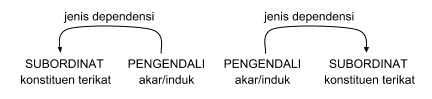
\includegraphics[width=0.6
	\textwidth] {pics/tautandependensi.png} \caption{Elemen-elemen dari tautan dependensi} 
\label{fig:tautandependensi} \end{figure}

Penguraian kalimat merupakan tahapan komputasional utama dalam tahap pengolahan data penelitian sesuai dengan teori yang dijabarkan pada bab sebelumnya. Pada penelitian ini, penguraian kalimat UDPipe mengadopsi Indonesian UD. Indonesian UD berisi kumpulan diagram pohon dependensi hasil konversi Universal Dependencies 2.0 \citep{nivre2017universal} yang dikondisikan khusus untuk Bahasa Indonesia. Anotasi tipe dependensi seperti pada contoh \pic~\ref{fig:contohtulis} dan \pic~\ref{fig:contohlisan} menyesuaikan dengan daftar anotasi dalam panduan dependensi milik \textit{universal Stanford Dependencies} (USD) \citep{de2014universal}. \pic~\ref{fig:contohtulis} dan \pic~\ref{fig:contohlisan} merupakan hasil visualisasi mandiri untuk memudahkan pemahaman tautan dependensi berdasarkan hasil penguraian dengan bantuan UDPipe. Kedua kalimat tersebut diambil dari korpus data ragam tulis dan lisan yang telah dibangun. UDPipe tidak memiliki masalah dalam pengolahan kedua contoh data dari ragam tulis dan lisan ini meskipun kedua contoh data tidak memiliki aktor pelaku. Namun, pada beberapa kalimat yang lain, UDPipe masih memiliki masalah dalam menguraikannya sehingga diperlukan tahapan verifikasi manual untuk memastikan kualitas data. Skema anotasi yang dihasilkan berdasarkan tahap penguraian kalimat ini bersifat lintas bahasa yang awalnya dikembangkan untuk Bahasa Inggris kemudian berkembang menjadi 60 bahasa, termasuk Bahasa Indonesia (\citealp{de2008stanford, de2014universal, nivre2017universal}). 

\begin{figure}
	\centering 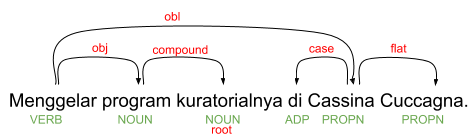
\includegraphics[width=0.5
	\textwidth] {pics/contohtulis.png} \caption{Contoh hasil penguraian kalimat untuk data ragam tulis} 
\label{fig:contohtulis} \end{figure}

\begin{figure}
	\centering 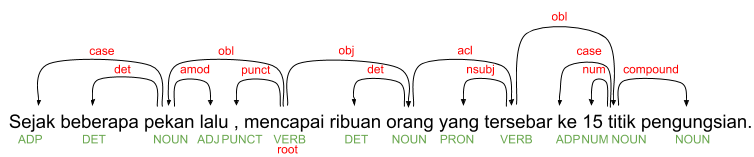
\includegraphics[width=0.85
	\textwidth] {pics/contohlisan.png} \caption{Contoh hasil penguraian kalimat untuk ragam lisan} 
\label{fig:contohlisan} \end{figure}

Kontekstualisasi treebank dependensi yang bersifat lintas bahasa dilakukan dengan melibatkan MorphInd \citep{larasati2011indonesian}, sebuah pendekatan morfologis dan penguraian lemma untuk pengolahan bahasa. MorphInd memiliki aturan morfofonemik dan morfosintaktis untuk menganalisis kata-kata Bahasa Indonesia yang mengalami infleksi dan derivasi. Hasil olahan MorphInd mengintegrasikan penandaan morfologis pada sebuah kata seperti pada \pic~\ref{fig:morphind_schema}.

\begin{figure}
	\centering 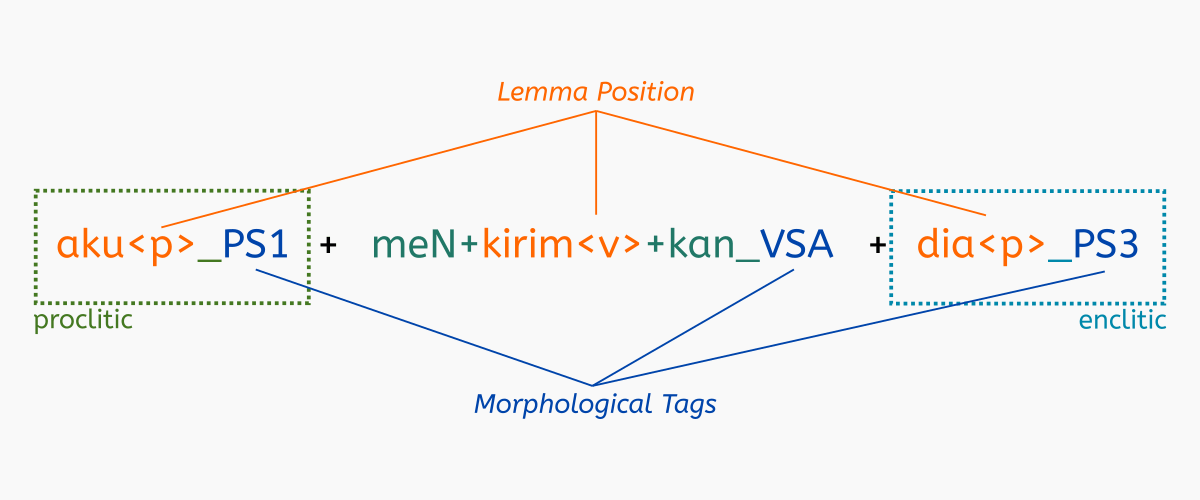
\includegraphics[width=1
	\textwidth] {pics/morphind_schema.png} \caption{Contoh hasil ekstraksi lemma dengan memanfaatkan MorphInd \citep{larasati2011indonesian} } 
\label{fig:morphind_schema} 
\end{figure}

Penelitian ini mengikuti panduan dependensi milik Stanford Parser \citep{de2008stanford} dan pengembangannya yaitu \textit{universal Stanford Dependencies} (USD) \citep{de2014universal} yang mengikutsertakan tanda baca yang terlibat dalam kalimat. Penelitian ini tidak mengikutsertakan tanda baca pada akhir kalimat dalam penghitungan jarak dependensi karena tanda baca di akhir kalimat tidak memberikan pengaruh terhadap jumlah tautan dependensi yang terjadi dalam sebuah kalimat. Namun, tanda baca pada akhir kalimat tetap diperhatikan untuk analisis karena dapat menjadi indikasi perbedaan jenis kalimat maka yang mendorong perbedaan perilaku tautan dependensi yang ada. Tanda baca koma yang mewakili jeda atau \textit{pause} dilibatkan dalam proses penguraian kalimat karena memiliki peran sintaktis yang harus diperhitungkan. Dependensi tipe Stanford \citep{de2008stanford} umumnya memilih konstituen kata penuh dibandingkan dengan konstituen kata tugas sebagai induk sintaktis, kecuali untuk konstruksi kopula (tergantung kasus) dan frasa adposisi seperti pada diagram pohon dependensi bahasa Indonesia dalam Universal Dependencies 2.0 \citep{nivre2017universal}. Berikut adalah deskripsi yang membandingkan kedua jenis konstituen kata tersebut berdasarkan Kamus Linguistik \citep{kridalaksana2008kamus}:

\begin{itemize}
	\item \textbf{kata penuh} (\textit{content word} atau \textit{full word}) merupakan kata yang mempunyai makna leksikal yang bebas seperti \textit{rumah}, \textit{angin}, \textit{orang}, dan lain sebagainya.
	\item \textbf{kata fungsi} (\textit{function word}) merupakan kata yang terutama menyatakan hubungan gramatikal yang tidak dapat bergabung dengan afiks, dan tidak mengandung makna antara lain adalah preposisi, konjungsi, artikel, dan pronomina.
\end{itemize}

\tab~\ref{tab:tipe_anotasi} berikut berisi kerangka anotasi berdasarkan \textit{universal Stanford Dependencies} (USD) \citep{de2014universal} yang juga menjadi ancangan untuk koleksi diagram pohon dependensi Universal Dependencies 2.0 \citep{nivre2017universal}.

\begin{table}
\begin{center}
\begin{footnotesize}
\caption{Kerangka anotasi berdasarkan \textit{universal Stanford Dependencies} (USD) \citep{de2014universal}} \label{tab:tipe_anotasi}
\begin{tabular}{ l l l }
    \hline

    \multicolumn{3}{ l }{\textbf{Konstituen terikat inti dari klausa predikat}} \\
    \textit{Nomina} & \textit{Verba} & \\
    nsubj & csubj & \\
    nsubjpass & csubjpass & \\
    dobj & ccomp & xcomp \\
    iobj & & \\
    \hline

    \multicolumn{3}{ l }{\textbf{Konstituen terikat bukan inti dari klausa predikat}} \\
    \textit{Nomina} & \textit{Verba} & \textit{Pewatas} \\
    & advcl & advmod \\
    & nfincl & neg \\
    nmod & ncmod &  \\
    \hline
    
    \multicolumn{3}{ l }{\textbf{Konstituen terikat klausa khusus }} \\
    \textit{Nomina} & \textit{Tambahan} & \textit{Lain-lain} \\
    vocative & aux & mark \\
    discourse & auxpass & punct \\
    expl & cop \\
    \hline
    
    \multicolumn{3}{ l }{\textbf{Koordinasi}} \\
    conj & cc \\
    \hline
    
    \multicolumn{3}{ l }{\textbf{Konstituen terikat nomina}} \\
    \textit{Nomina} & \textit{Verba} & \textit{Pewatas} \\
    nummod & relcl & amod \\
    appos & nfincl & det \\
    nmod & ncmod & neg \\
    \hline
    
    \multicolumn{3}{ l }{\textbf{Penggabungan dan non-kategoris}} \\
    compound & mwe & goeswith \\
    name & foreign \\
    \hline
    
    \multicolumn{3}{ l }{\textbf{Konstituen penanda, preposisi, penanda posesif}} \\
    case \\
    \hline
    
    \multicolumn{3}{ l }{\textbf{Penggabungan relasi lepas }} \\
    list & parataxis & remnant \\
    dislocated & & reparandum \\
    \hline
    
    \multicolumn{3}{ l }{\textbf{Lain-lain}} \\
    \textit{Akar kalimat} & \textit{Dependensi non-kategoris} \\
    root dep \\
    \hline

\end{tabular}
\end{footnotesize}
\end{center}
\end{table}


Tipe-tipe dependensi dalam \textit{universal Stanford Dependencies} (USD) \citep{de2014universal} tersebut masih terus dalam pengembangan dan penyempurnaan sehingga memerlukan banyak penelitian dukungan terutama pada tipe-tipe dependensi yang kontekstual terhadap bahasa lokal. Berikut adalah penjabaran mengenai tipe-tipe dependensi yang utama:

\begin{figure}
	\centering 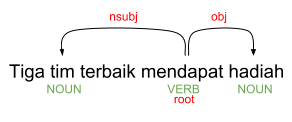
\includegraphics[width=0.4
	\textwidth] {pics/anotasiroot.png} \caption{Contoh anotasi akar (\textit{root}), \textit{nsubj}, dan \textit{obj}} 
\label{fig:anotasiroot} 
\end{figure}

\begin{itemize}
\item $root$ mengacu pada akar dari sebuah kalimat. Dalam pengindeksan sebuah kalimat, $root$ ditandai dengan indeks 0 sehingga pengindeksan kata lain yang diikat oleh akar dimulai dari indeks 1. Setiap diagram pohon dependensi hanya memiliki satu $root$. Jika predikat utama tidak hadir, dan kalimat tersebut memiliki banyak simpai percabangan yang sifatnya terikat, maka salah satu dari simpai cabang tersebut akan diindekskan menjadi $root$.
\item $nsubj$ merupakan subyek sintaktis nomina yang berperan sebagai aktor pelaku atau memiliki kualitas aktor pelaku. Ketidakhadiran nomina utama dapat menyebabkan anotasi $nsubj$ jatuh pada pronomina atau pronomina relatif. $nsubj$ juga digunakan sebagai subyek nomina dari verba pasif. Pengendali dari $nsubj$ tidak harus verba. Saat verba ditandai oleh kopula, maka akar klausa merupakan pelengkap kopula tersebut (yang dapat berupa adjektiva atau nomina). Sementara, $csubj$ merupakan subyek sintaktis dari sebuah klausa dalam arti bahwa subyek tersebut adalah klausa itu sendiri. Pengendali dari tipe dependensi ini tidak harus verba seperti pada $nsubj$. Subyek sintaktis klausal ini bergantung pada verba leksikal utama atau predikat lain dari klausa tempatnya bergantung. Dalam keadaan pasif, $csubj$ memiliki karakteristik serupa $nsubj$.
\item $obj$ adalah obyek dari verba yang juga merupakan bagian paling penting terutama dalam melihat valensi verbal. Umumnya, $obj$ merupakan anotasi dari frasa nomina.
\end{itemize}

\begin{figure}
	\centering 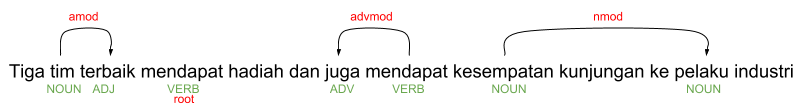
\includegraphics[width=1
	\textwidth] {pics/anotasiamod.png} \caption{Contoh anotasi \textit{amod}, \textit{nmod}, dan \textit{advmod}} 
\label{fig:anotasiamod} 
\end{figure}

\begin{itemize}
\item $amod$ merupakan pewatas adjektiva dari nomina. Tipe dependensi ini menandakan bahwa adjektiva tersebut memodifikasi makna sebuah nomina.
\item $nmod$ adalah tipe dependensi yang digunakan untuk nomina terikat dari dari nomina lain atau frasa nomina dan berkorespondensi (secara fungsi) dengan pelengkap atributif atau genitif. Serupa dengan $nmod$, $obl$ merupakan nomina yang berfungsi sebagai argumen tambahan atau pelengkap dan berkorespondensi dengan adverbia. 
\item $advmod$ mewakili pewatas adverbia dari sebuah konstituen yang merupakan adverbia atau frasa adverbia yang memilik fungsi untuk memodifikasi predikat. Dalam standar USD, pewatas dari predikat (definisi adverbia yang spesifik) dengan pewatas dari kelas kata lain seperti adjektiva dan adverbia. Semua fungsi-fungsi ini dimasukkan ke bawah anotasi $advmod$. 
\end{itemize}

\begin{figure}
	\centering 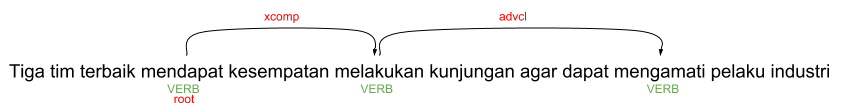
\includegraphics[width=1
	\textwidth] {pics/anotasixcomp.png} \caption{Contoh anotasi \textit{xcomp}, dan \textit{advcl}} 
\label{fig:anotasixcomp} 
\end{figure}

\begin{itemize}
\item $xcomp$ mewakili pelengkap klausal sebuah verba atau adjektiva dari argumen utama pada tingkat yang sama dengan subyek atau obyek utama. Namun, apaibla pelengkap klausal tidak berada pada tingkat yang sama dengan subyek atau obyek utama, maka tipe dependensi yang lebih tepat adalah $ccomp$.
\item  $advcl$ digunakan untuk klausa finit maupun non-finit yang memodifikasi predikat. Sementara, $acl$ merupakan anotasi untuk klausa finit maupun non-finit yang memodifikasi nomina. Induk dari $acl$ merupakan nomina yang termodifikasi, dan konstituen terikat dari tipe tautan ini adalah kepala klausa yang memodifikasi nomina tersebut.
\end{itemize}

\begin{figure}
	\centering 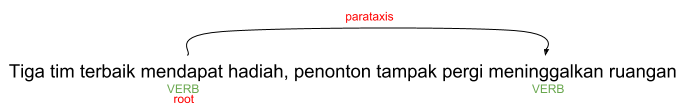
\includegraphics[width=0.9
	\textwidth] {pics/anotasiparataxis.png} \caption{Contoh anotasi \textit{parataxis}} 
\label{fig:anotasiparataxis} 
\end{figure}

\begin{itemize}
\item $parataxis$ berasal dari kata Yunani yang berarti 'ditempatkan berdampingan'. Tipe dependensi ini adalah relasi antara sebuah konstituen (yang umumnya predikat utama dalam kalimat) dengan elemen lain yang ditempatkan tanpa koordinasi maupun relasi argumen dengan induk yang eksplisit. $parataxis$ merupakan koordinasi yang menyerupai diskursus sehingga memiliki kemampuan untuk menjadi kalimat lepas yang dapat berdiri sendiri. Tipe dependensi ini juga berlaku pada relasi antara kutipan dan klausa utama serta penjelasan yang umumnya berada di dalam kurung.
\end{itemize}

\begin{figure}
	\centering 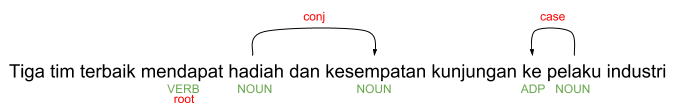
\includegraphics[width=0.9
	\textwidth] {pics/anotasiconj.png} \caption{Contoh anotasi \textit{conj}, dan \textit{case}} 
\label{fig:anotasiconj} 
\end{figure}

\begin{itemize}
\item $conj$ adalah singkatan dari konjungsi yang merupakan tipe dependensi antara dua konstituen yang dihubungkan oleh konjungsi koordinatif seperti \textit{dan}, \textit{atau}, dan lain-lain. Konjungsi diperlakukan secara asimetris dengan konstituen yang direalisasikan terlebih dahulu sebagai induk tautannya.
\item $case$ merupakan tipe yang digunakan untuk menandai konstituen yang diperlakukan sebagai kata sintaktis terpisah seperti preposisi. Konstituen penanda ini diperlakukan sebagai konstituen terikat dari nomina yang mengikatnya atau konstituen yang diperkenalkannya. Serupa dengan $case$, tipe dependensi $mark$ menandakan klausa finit yang merupakan subordinat dari klausa lain. Umumnya ditandai dengan kata-kata seperti \textit{setelah}, \textit{namun}, \textit{meskipun}, tetapi dapat juga ditandai oleh konstituen yang menjadi argumen utamanya.
\end{itemize}


%-----------------------------------------------------------------------------%
\subsection{Anotasi nilai panjang dependensi kalimat dan rata-rata jarak dependensi antarkonstituen}
%-----------------------------------------------------------------------------%
Setelah kedua korpus data diuraikan dengan pendekatan komputasional, tabel hasil penguraian data diberikan anotasi kolom tambahan berisi anotasi nilai hasil penghitungan panjang dependensi kalimat (yang selanjutnya disingkat menjadi DL) dan rata-rata jarak dependensi antarkonstituen (yang selanjutnya disingkat menjadi MDD). Anotasi ini dilakukan tidak hanya pada masing-masing kalimat, namun juga pada masing-masing relasi yang ada dalam kalimat tersebut. Penghitungan untuk mendapatkan nilai DL dan MDD tergabung menjadi dua tahapan yang berkelanjutan karena untuk mendapatkan nilai MDD, dibutuhkan nilai DL terlebih dahulu. Langkah pertama dalam tahapan anotasi nilai DL dan MDD ini adalah menguraikan kalimat di dalam kedua korpus sesuai prinsip penghitungan panjang dan jarak dependensi. Seluruh kalimat di dalam kedua korpus diperlakukan sebagai deretan konstituen $W1...Wi...Wn$. Jarak dependensi (yang selanjutnya disingkat menjadi DD) antara konstituen $Wa$ dengan konstituen $Wb$ dapat dihitung dari selisih keduanya (\citealp{liu2008dependency, liu2017dependency, futrell2015large}) sehingga konstituen-konstituen yang bersebelahan atau berdampingan memiliki jarak dependensi sejumlah 1. Untuk memperhitungkan arah dependensi dalam penghitungan ini, selisih antara kedua konstituen perlu dibedakan menyesuaikan dengan arah panah tautan dependensi tersebut:
\begin{itemize}
\item Apabila $a$ merupakan induk dan posisinya sebelum $b$ yang merupakan konstituen terikatnya, maka anotasi yang diberikan bernilai \textbf{positif}.
\item Sedangkan, apabila $a$ merupakan induk dan posisinya berada setelah $b$ yang merupakan konstituen terikatnya, maka anotasi yang diberikan bernilai \textbf{negatif}. 
\end{itemize}
Dalam melihat kecenderungan Pengurangan Panjang Dependensi (DLM), nilai yang dianalisis adalah nilai Panjang Dependensi atau DL. DL didapatkan dengan menjumlahkan semua nilai DD dalam satu kalimat (\citealp{gildea2010grammars, futrell2015large}) dengan rumus sebagai berikut: 

\noindent \begin{align}\label{eq:bola}
	\displaystyle\sum_{i=1}^{n-1} |DD_i|
\end{align}

Penelitian ini juga melihat kecenderungan Pengurangan Jarak Dependensi (DDM) dengan menganalisis nilai Rata-rata Jarak Dependensi (MDD) (\citealp{liu2008dependency, liu2017dependency}) dengan rumus sebagai berikut:

\noindent \begin{align}\label{eq:bola}
	\frac{1}{n-1} \displaystyle\sum_{i=1}^{n-1} |DD_i|
\end{align}

Pada kedua rumus tersebut, $n$ adalah jumlah konstituen di sebuah kelimat. $DDi$ adalah jarak dependensi dengan tautan sejumlah $i$. Dalam kata lain, MDD didapatkan dari nilai DL (yang merupakan jumlah dari nilai absolut DD dalam sebuah kalimat) dibagi dengan jumlah tautan dependensi dalam kalimat tersebut. Berdasarkan dua kalimat contoh dari data ragam tulis (\pic~\ref{fig:contohtulis}) dan ragam lisan (\pic~\ref{fig:contohlisan}) di atas, maka anotasi nilai DL dan MDD digambarkan pada visualisasi mandiri seperti pada \pic~\ref{fig:contohtulis_DLMDD} dan \pic~\ref{fig:contohlisan_DLMDD}.

\begin{figure}
	\centering 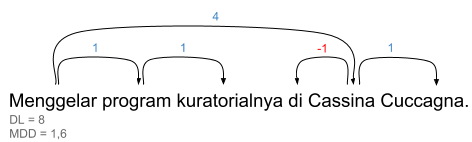
\includegraphics[width=0.5
	\textwidth] {pics/contohtulis_DLMDD.png} \caption{Contoh hasil olahan penghitungan jarak antarkata data ragam tulis} 
\label{fig:contohtulis_DLMDD} 
\end{figure}

\begin{figure}
	\centering 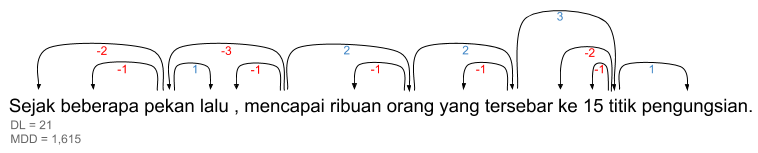
\includegraphics[width=0.85
	\textwidth] {pics/contohlisan_DLMDD.png} \caption{Contoh hasil olahan penghitungan jarak antarkata data ragam lisan} 
\label{fig:contohlisan_DLMDD} 
\end{figure}

Pada contoh di atas, kalimat dari ragam tulis pada \pic~\ref{fig:contohtulis_DLMDD} memiliki nilai DL (atau total nilai DD dalam kalimat tersebut) sejumlah 8 dan jumlah tautan dependensi sebanyak 5 sehingga nilai MDD yang didapat adalah 1,6. Hal ini berarti rata-rata jarak antara dua konstituen dalam kalimat tersebut adalah sejauh 1,6 konstituen. Kalimat ini memiliki empat tautan positif (induk sebelum konstituen terikat) dan satu tautan negatif (induk setelah konstituen terikat), yaitu pada relasi antara \textit{Cassina} dan \textit{di}. Karena jumlah konstituen dalam kalimat ini di bawah 10 konstituen, maka kalimat ragam tulis ini masuk ke dalam klasifikasi kalimat pendek. Sedangkan, kalimat dari ragam lisan \pic~\ref{fig:contohlisan_DLMDD} memiliki nilai DL sejumlah 21 dan jumlah tautan dependensi sebanyak 13 sehingga nilai MDD yang didapat adalah 1.615 yang berarti rata-rata jarak antara dua konstituen dalam kalimat tersebut adalah sejauh 1,615 konstituen. Kalimat ragam lisan tersebut masuk ke dalam klasifikasi data ragam lisan dengan panjang kalimat di atas 20 konstituen atau klasifikasi kalimat panjang. Berbeda dengan contoh ragam tulis, kalimat ini memperlihatkan jumlah tautan negatif yang lebih banyak dibandingkan tautan positif.

%-----------------------------------------------------------------------------%
\subsection{Klasifikasi data}
%-----------------------------------------------------------------------------%
Salah satu penjabaran pokok permasalahan menitikberatkan pada pengaruh panjang kalimat dalam penyusunan struktur kalimat yang efisien dalam bahasa Indonesia dipandang dari segi dependensi. Tidak hanya dari segi panjang kalimat, penelitian ini juga menitikberatkan pada perbandingan perilaku dependensi dalam ujaran yang formal dan ujaran yang lebih spontan. Kedua aspek ini diwakili oleh jenis ragam yaitu tulis dan lisan. Berikut adalah kriteria utama untuk tahap klasifikasi terhadap keseluruhan data.

\begin{itemize}
	\item Untuk melihat perbandingan dasar antara ujaran formal dengan ujaran yang lebih spontan, maka data korpus perlu diklasifikasikan menjadi dua, yaitu data ragam tulis dan ragam lisan.
	\item Terkait dengan uraian permasalahan mengenai pengaruh panjang kalimat dalam penyusunan struktur kalimat yang mungkin juga mempengaruhi jarak dan arah dependensi, maka data korpus akan diklasifikasikan menjadi tiga berdasarkan panjang kalimat di bawah 10 konstituen (dikategorikan sebagai kalimat pendek), 11 hingga 20 konstituen (dikategorikan sebagai kalimat menengah), dan di atas 20 koonstituen (dikategorikan sebagai kalimat panjang). Pendekatan ini menindaklanjuti temuan penelitian \cite{oya2011syntactic} serta \cite{jiang2015effects} yang menggunakan klasifikasi serupa. 
\end{itemize}

Kedua poin ini mendasari langkah klasifikasi terhadap kedua korpus data untuk memudahkan proses agregasi data dalam langkah analisis berikutnya (Tabel \ref{tab:tabel_klasifikasi_data}). 

\begin{table}
\begin{footnotesize}
\begin{center}
  \caption{Klasifikasi data penelitian}\label{tab:tabel_klasifikasi_data}
  \begin{tabular}{ | p{3cm} | c | c | c |}
    \hline
    Ragam / Panjang kalimat & \textless 10 konstituen & 11 - 20 konstituen & \textgreater 20 konstituen \\ \hline
    Tulis & Tulis \textless 10 konstituen & Tulis 11 - 20 konstituen & Tulis \textgreater 20 konstituen  \\ \hline
    Lisan & Lisan \textless 10 konstituen & Lisan 11 - 20 konstituen & Lisan \textgreater 20 konstituen \\
    \hline
  \end{tabular}
\end{center}
\end{footnotesize}
\end{table}

%-----------------------------------------------------------------------------%
\section{Teknik analisis data}
%-----------------------------------------------------------------------------%

Serangkaian tahapan analisis data dengan pendekatan kuantitatif dan kualitatif dilakukan untuk mendapatkan gambaran awal mengenai fenomena efisiensi kalimat dalam bahasa Indonesia dipandang dari segi dependensi serta strategi-strategi yang mungkin diterapkan oleh penutur untuk menghasilkan efisiensi tersebut. Sejauh pemahaman saya dari hasil tinjauan terhadap penelitian-penelitian terdahulu, penelitian ini merupakan penelitian pertama yang mencoba untuk memberikan wawasan linguistik terhadap masalah tersebut sehingga beberapa metode-metode analisis yang diterapkan untuk menganalisis hasil olahan data bersifat eksperimental karena mengadopsi pendekatan yang sebelumnya menggunakan data bahasa lain. Tahap analisis ini diawali dengan uji hipotesis fenomena DLM dalam bahasa Indonesia untuk memberikan bukti empiris adanya efisiensi kalimat berdasarkan korpus data yang dikumpulkan. Langkah-langkah selanjutnya menggabungkan ancangan kuantitatif dan kualitatif untuk membedah hasil olahan data sesuai dengan pokok permasalahan penelitian yang diajukan pada Bab 1.

%-----------------------------------------------------------------------------%
\subsection{Percobaan acak untuk menguji hipotesis DLM dalam bahasa Indonesia}
%-----------------------------------------------------------------------------%
Sebelum melakukan identifikasi terhadap karakteristik struktur dependensi berdasarkan korpus data yang dikumpulkan, perlu dilakukan uji hipotesis terhadap asumsi adanya efisiensi kalimat dalam bahasa Indonesia dari segi dependensi. Sebelumnya, uji hipotesis efisiensi kalimat dengan melihat nilai DLM pada bahasa Indonesia pernah dilakukan oleh \cite{futrell2015large} secara lintas bahasa. Namun, percobaan yang dilakukan \cite{futrell2015large} menggunakan korpus data yang berbeda, yaitu data ragam tulis dalam berbagai aliran teks seperti artikel penelitian, \textit{blog}, artikel berita, dan data dari media sosial. Penelitian ini mengadopsi pendekatan percobaan acak yang dilakukan oleh \cite{futrell2015large} dan \cite{gildea2010grammars}. \cite{futrell2015large} menyebut algoritma acak ini dengan istilah \textit{Free Word Order Baseline}, sedangkan \cite{gildea2010grammars} menyebut algoritma acak ini dengan istilah \textit{unlabeled Dependency Linearization Algorithm} (\textit{unlabeled} DLA). Secara prinsip, kedua algoritma ini memiliki kesamaan, yaitu kedua algoritma acak tersebut menyusun ulang konstituen-konstituen dalam kalimat tanpa memperhitungkan aturan tata bahasa yang ada. Sebagai contoh, tidak ada konsistensi apakah aktor pelaku mendahului atau berada setelah verba. Perbedaan kedua algoritma ini terletak pada penerapan algoritma tersebut. 

\cite{gildea2010grammars} menggunakan algoritma \textit{unlabeled} DLA untuk mengubah bentuk kalimat hasil observasi $U$ menjadi bentuk kalimat acak baru dengan nilai DL yang paling kecil $Umin$ dalam arti $Umin$ merupakan bentuk paling efisien (dari segi dependensi) dari $U$ dan membandingkan nilai DL yang didapatkan keduanya. Sementara, \cite{futrell2015large} menerapkan algoritma acaknya terhadap $U$ sebanyak 100 kali untuk menghasilkan kalimat dengan nilai-nilai DL baru dari $U1$ hingga $U100$. \cite{futrell2015large} dan \cite{gildea2010grammars} menyebutkan bahwa $Umin$ yang dihasilkan mungkin tidak bersifat gramatikal maupun berterima. Namun, \cite{futrell2015large} juga menyebutkan pengecualian terhadap bahasa Indonesia yang menghasilkan $Umin$ yang sangat mendekati $U$. Langkah-langkah yang dilakukan dalam algoritma acak ini dijabarkan sebagai berikut:
\begin{enumerate}
\item Identifikasi akar dan semua konstituen terikat yang memiliki tautan dependensi langsung terhadap akar tersebut (level simpai pusat).
\item Penyusunan acak terhadap urutan konstituen pada level simpai pusat.
\item Identifikasi konstituen terikat yang merupakan induk terhadap konstituen terikat lain (level simpai cabang).
\item Penyusunan acak terhadap urutan konstituen pada level simpai cabang.
\item Pengulangan proses pada induk di simpai-simpai cabang berikutnya.
\end{enumerate}
Poses tersebut akan menghasilkan $U1$ sehingga diulang sebanyak 100 kali untuk menghasilkan 100 kalimat dengan susunan acak \citep{futrell2015large}. Berdasarkan tinjauan terhadap kedua pendekatan tersebut dan temuan mengenai data bahasa Indonesia yang didapatkan \cite{futrell2015large}, penelitian ini mengadopsi pendekatan algoritma acak yang dilakukan oleh \cite{futrell2015large}.

Analisis terhadap percobaan acak dilakukan juga dengan mempertimbangkan panjang kalimat yang terkontrol (\textit{controlled sentence length}) antara korpus data hasil observasi dan korpus data kalimat acak. Hal ini dilakukan berdasarkan argumen signifikansi dalam menganalisis dengan panjang kalimat terkontrol sempat dikemukakan oleh \cite{ferrer2014risks} dan \cite{jiang2015effects} serta keterbatasan kapasitas komputasi untuk mengolah korpus berskala besar. Oleh karena itu, percobaan ini dilakukan sebanyak enam kali untuk panjang kalimat dengan frekuensi terbanyak pada masing-masing klasifikasi dari setiap ragam. Perbandingan nilai DL dari korpus data hasil observasi dan korpus data hasil percobaan acak kemudian divisualisasikan melalui histogram dari keduanya. Algoritma acak untuk percobaan ini dijalankan pada bahasa pemrograman Python (versi 3.6.3) (Python Core Team, 2017) kemudian dianalisis dan divisualisasikan pada bahasa pemrograman R (versi 3.3.3) \citep{r2017project} dengan menggunakan paket CRAN untuk visualisasi Plotly \citep{sievert2017plotly}).

Dalam meguji hipotesis DLM, penelitian ini menggunakan uji beda rata-rata dua populasi berbeda di mana nilai varians populasi diketahui (\textit{z-test}). Syarat untuk meakukan \textit{z-test} ini adalah asumsi dasar bahwa kedua populasi memiliki distribusi normal, dan varians dari kedua distribusi diketahui berbeda antara populasi pertama dan kedua. Jika diasumsikan bahwa $\mu_1$ dan $\mu_2$ merepresentasikan kedua proporsi rata-rata dari dua populasi dan $\delta=\mu_1 - \mu_2$, maka hipotesis nol untuk membandingkan kedua rata-rata adalah $H_0:\delta=0$. Hipotesis alternatif dapat berupa salah satu dari $H_1:\delta \neq0$, $H_1:\delta \textgreater0$, dan $H_1:\delta \textless0$. Formula untuk \textit{z-test} dapat didefinisikan sebagai berikut:

\begin{equation}
z=\frac{
	\bar{x}_1 - \bar{x}_2}{
	\sqrt{\frac{\sigma_1^2}{n_1} + \frac{\sigma_2^2}{n_2}}
	}
\end{equation}
di mana $x$ adalah rata-rata distribusi nilai, $n$ merupakan banyaknya sampel, dan $\sigma$ adalah deviasi standar populasi yang diketahui. Daerah kritis adalah daerah yang digunakan untuk menolak atau tidak menolak hipotesis nol. Titik kritis untuk menentukan keputusan ini adalah:\\
untuk $H_1:\delta \neq0$
\begin{equation}
z \textless z_{\alpha / 2}
\quad\mathrm{atau}\quad 
 z \textgreater z_{1-\alpha / 2},
\end{equation}
untuk $H_1:\delta \textgreater0$
\begin{equation}
 z \textgreater z_{1-\alpha},
\end{equation}
untuk $H_1:\delta \textless0$
\begin{equation}
 z \textless z_{\alpha}.
\end{equation}
Tingkat signifikansi ($\alpha$) atau \textit{p-value} yang digunakan adalah nilai 0,05 dan 0,001 untuk kemungkinan yang lebih ekstrim. 

%-----------------------------------------------------------------------------%
\subsection{Analisis pengaruh persebaran panjang kalimat terhadap panjang dan jarak dependensi}
%-----------------------------------------------------------------------------%
Sebelum tahap ini, seluruh kalimat dalam kedua korpus data telah melalui penghitungan nilai DL dan MDD dan telah diklasifikasi berdasarkan panjang kalimatnya. Analisis pengaruh persebaran panjang kalimat terhadap efisiensi kalimat mencoba melihat relasi yang terjadi antara panjang kalimat dan nilai DL serta MDD yang didapatkan. Seperti yang dijelaskan sebelumnya, pertimbangan untuk mencari nilai DL dan MDD menitikberatkan pada dua hal yang sedikit berbeda sehingga pada tahap ini, kedua nilai dipaparkan karena diduga mengandung informasi yang berbeda juga. Tahap ini juga memperhitungkan spontanitas ujaran sehingga perbandingan nilai DL dan MDD antara ragam tulis dan lisan penting untuk dianalisis. 

Langkah pertama yang dilakukan adalah membandingkan persebaran frekuensi panjang kalimat secara keseluruhan antara kedua korpus data dan menganalisis perbandingan tersebut untuk melihat adanya kecenderungan terhadap panjang kalimat secara umum. Langkah berikutnya adalah memisahkan korpus data pada setiap ragam menjadi tiga korpus yang lebih kecil sesuai dengan klasifikasi panjang kalimatnya yaitu kalimat pendek (maksimal 10 konstituen), kalimat menengah (11 hingga 20 konstituen), dan kalimat panjang (minimal 21 konstituen). Sehingga, didapatkan enam korpus yang lebih kecil dari kedua ragam ujaran. Kemudian, rata-rata (\textit{mean}) dihitung berdasarkan nilai-nilai DL dan MDD yang didapatkan oleh setiap kalimat dari korpus-korpus tersebut dan dipaparkan sesuai dengan masing-masing klasifikasi. 

Perbandingan antara nilai-nilai dari masing-masing klasifikasi pada data ragam tulis dengan data ragam lisan dianalisis untuk melihat adanya perbedaan perilaku efisiensi kalimat (\gls{dlm} dan \gls{ddm}). Uji hipotesis pada bagian analisis ini juga menggunakan uji beda rata-rata dua populasi berbeda di mana nilai varians populasi diketahui (\textit{z-test}). Analisis kualitatif dilakukan untuk melihat adanya perbedaan struktur kalimat pada masing-masing klasifikasi atau antara kedua korpus data.

%-----------------------------------------------------------------------------%
\subsection{Analisis arah dependensi dan direksionalitas induk}
%-----------------------------------------------------------------------------%
Salah satu pertanyaan penelitian menitikberatkan pada jarak dan arah dependensi yang muncul berdasarkan data yang dikumpulkan. Arah dependensi berkaitan dengan hierarki relasi antara induk dan konstituen terikatnya. Seperti yang dijelaskan pada bab sebelumnya dan divisualisasikan pada \pic~\ref{fig:tautandependensi}, relasi antara dua konstituen dihubungkan dengan sebuah tautan yang memiliki panah. Arah panah tersebut merepresentasikan hierarki relasi antara keduanya. Arah panah ke kanan menandakan tautan yang bernilai positif, dan sebaliknya, arah panah ke kiri menandakan tautan yang bernilai negatif. Hal ini dapat dilihat juga pada visualisasi dari dua kalimat contoh yang diambil dari data ragam tulis (\pic~\ref{fig:contohtulis}) dan ragam lisan (\pic~\ref{fig:contohlisan}). Kedua visualisasi ini mengandung nilai-nilai tautan dengan anotasi positif ($+$) dan anotasi negatif ($-$) (yang juga dibedakan oleh warna biru dan merah) untuk memberikan gambaran terhadap perbedaan arah tautan dependensi dalam sebuah kalimat. Sebagai contoh, \pic~\ref{fig:contohtulis} memiliki 4 tautan positif dan 1 tautan negatif, sehingga pada kalimat ini relasi di mana induk direalisasikan sebelum konstituen terikat mendominasi kalimat tersebut. Pada level dependensi utama atau simpai pusat, \textit{menggelar} memiliki 2 tautan positif terhadap \textit{program} dan \textit{Cassina} serta 0 tautan negatif.

Simpai pusat merepresentasikan relasi-relasi utama dalam sebuah kalimat berdasarkan dependensi. Pada kalimat yang lebih kompleks, simpai pusat juga memberikan gambaran terhadap relasi-relasi utama, namun terkadang banyak relasi pada cabang yang tidak terwakili. Oleh karena itu, pemaparan kedua analisis arah dependensi pada relasi-relasi secara keseluruhan dan pada simpai pusat penting untuk disampaikan. Pada tahap anotasi nilai DL, setiap relasi antara dua konstituen dalam sebuah kalimat sudah diberikan anotasi positif maupun negatif. Sehingga, pada tahap ini hanya perlu dilakukan agregasi data terhadap relasi-relasi bernilai positif dan relasi-relasi bernilai negatif. Tahap analisis ini didasarkan pada pembahasan mengenai percabangan searah dan percabangan beda arah yang dibahas oleh \cite{temperley2008dependency} dan \cite{dryer1992greenbergian} untuk melihat adanya kecenderungan dalam menerapkan tipe percabangan keduanya. Uji hipotesis untuk bagian analisis ini dilakukan dengan pendekatan penghitungan statistika deskriptif.

%-----------------------------------------------------------------------------%
\subsection{Pengamatan perubahan valensi akar verbal}
%-----------------------------------------------------------------------------%
Tahap analisis ini masih berkaitan erat dengan analisis arah dependensi karena keterkaitan valensi konstituen dalam sebuah kalimat dengan efisiensi kalimat tersebut tidak hanya dapat diamati melalui pengurangan nilai valensi. Sebuah konstituen dapat mempertahankan nilai valensinya tetapi tetap menghasilkan kalimat yang efisien, yaitu dengan mengatur letak konstituen yang diikatnya sehingga menempati posisi yang paling optimal (menghasilkan nilai DL terkecil). Analisis ini saya lakukan untuk melihat tautan dependensi dan hubungan induk dengan konstituen terikat secara lebih dekat terutama terkait kecenderungan penutur dalam menghasilkan kalimat yang efisien. Meskipun penelitian ini tidak menganalisis leksikon, prinsip dasar yang membentuk kemungkinan pola valensi dalam \textit{Probabilistic Valency Pattern} (PVP) \citep{liu2006syntactic} menjadi dasar pengamatan ini. Perlu saya tekankan bahwa \cite{liu2006syntactic} menganggap valensi sebagai kapasitas sebuah konstituen yang memiliki kualitas gabungan (\textit{combinatorial}). Hal ini berarti sebuah konstituen memiliki valensi tertentu dalam arti dapat mengikat konstituen lain, tetapi juga dapat bertindak sebagai konstituen yang diikat oleh induk lain. Penelitian ini mengamati valensi akar verbal pada simpai pusat pada tataran kalimat sehingga tidak ada aspek konstituen tersebut sebagai konstituen yang diikat induk lain karena dalam kalimat tersebut, konstituen yang diamati berada di posisi teratas dari hierarki dependensi.

Karena keterbatasan sumber daya linguistik untuk menganalisis valensi secara menyeluruh, pengamatan ini dilakukan secara manual dengan analisis kualitatif berdasarkan konsep PVP \citep{liu2006syntactic}. Contoh kalimat ragam tulis dan lisan pada \pic~\ref{fig:contohtulis} dan \pic~\ref{fig:contohlisan} dapat digunakan untuk mengilustrasikan analisis valensi akar verbal. Apabila disesuaikan dengan tata bahasa yang berlaku dalam bahasa Indonesia, kata \textit{menggelar} pada kalimat \textit{Menggelar program kuratorialnya di Cassina Cuccagna} dan kata \textit{mencapai} pada kalimat \textit{Sejak beberapa pekan yang lalu, mencapai ribuan orang yang tersebar ke-15 titik pengungsian} sama-sama tidak memiliki aktor pelaku sebagai konstituen terikatnya. Kata \textit{menggelar} mengikat satu konstituen pelengkap \textit{program (kuratorialnya)} dan satu konstituen keterangan \textit{Cassina (Cucigna)}, sementara kata \textit{mencapai} juga mengikat satu konstituen pelengkap \textit{(ribuan) orang} dan satu konstituen keterangan \textit{pekan (lalu)}. Temuan menarik pada \pic~\ref{fig:contohtulis} adalah partikel posesif \textit{-nya} yang tergabung pada frasa nomina modikatif posesif \textit{program kuratorialnya} mengindikasikan aktor pelaku yang tidak direalisasikan secara terpisah. 

%-----------------------------------------------------------------------------%
\chapter{\babEmpat} \label{chap:analisis}
%-----------------------------------------------------------------------------%

%-----------------------------------------------------------------------------%
\section{Pengantar}
%-----------------------------------------------------------------------------%
Pada bab ini, analisis korpus data jurnalistik Bahasa Indonesia termutakhir ragam tulis dan lisan dijabarkan melalui beberapa tahap. Kedua korpus dianalisis secara terpisah agar temuan analisis dapat disandingkan untuk melihat perbedaan karakter serta signifikansi perbedaan tersebut antara data ragam tulis dan ragam lisan. Tahap pertama merupakan proses penguraian kalimat dengan metode komputasional berdasarkan dependensinya. Merujuk pada penjelasan dalam Bab 3, penguraian kalimat ini dilakukan dengan bantuan sebuah kerangka kerja yang dapat dilatih ulang untuk pengkategorian token, penguraian lemma, dan penguraian kalimat bernama UDPipe \citep{udpipe2017}. Tahap kedua adalah proses penghitungan untuk mendapatkan panjang dependensi kalimat (DL) dengan pendekatan yang diadopsi dari penelitian \cite{gildea2010grammars} dan \cite{futrell2015large} serta rata-rata jarak dependensi antarkonstituen (MDD) dengan pendekatan yang diadopsi dari penelitian \cite{liu2017dependency}. Kemudian, pada tahap ketiga dilakukan percobaan acak dengan mengadopsi prinsip langkah-langkah \textit{Free Word Order Baseline} \citep{futrell2015large} terhadap tabel yang dihasilkan dari tahap-tahap sebelumnya. Tahap terakhir melibatkan penghitungan statistika deskriptif dan analisis secara kualitatif terhadap kalimat-kalimat di dalam kedua korpus yang mewakili aspek-aspek temuan penelitian berdasarkan analisis kuantitatif.

%-----------------------------------------------------------------------------%
\section{Prosedur analisis}
%-----------------------------------------------------------------------------%
Pada tahap pertama, kedua korpus data jurnalistik dipersiapkan untuk dapat diolah dengan metode komputasional. Dalam data ragam lisan ditemukan beberapa kalimat yang tidak lengkap. Karena metode penguraian kalimat belum dapat mengolah kalimat seperti ini, kalimat-kalimat tidak lengkap dikeluarkan dari korpus terlebih dahulu agar tidak mempengaruhi hasil penghitungan secara keseluruhan. Untuk memastikan kualitas penguraian kalimat dan anotasi yang sesuai dengan standar analisis, dilakukan tahap tambahan yaitu pemeriksaan secara manual. Berdasarkan pemeriksaan ini, kualitas penguraian kalimat untuk data ragam tulis terbilang sudah bagus, namun pada ragam lisan masih diperlukan pengembangan terutama untuk kata-kata informal atau sehari-hari. 

\begin{center}
\begin{table} \caption{Penggalan penguraian kalimat diambil dari korpus yang dianalisis}\label{tab:penggalan_kalimat}
\begin{tiny}
  \begin{tabulary}{1\textwidth}{| L | L | L | L | L | L | L |}
  \hline
    type & sentence & token & upos & relation & token id & head token id \\ \hline
tulis & Mengingat fungsi dari telepon seluler tersebut sebagai sarana komunikasi yang berdampak pada peningkatan perekonomian & Mengingat & VERB & root & 1 & 0 \\ \hline
tulis & Mengingat fungsi dari telepon seluler tersebut sebagai sarana komunikasi yang berdampak pada peningkatan perekonomian & fungsi & NOUN & obj & 2 & 1 \\ \hline
tulis & Mengingat fungsi dari telepon seluler tersebut sebagai sarana komunikasi yang berdampak pada peningkatan perekonomian & dari & ADP & case & 3 & 4 \\ \hline
tulis & Mengingat fungsi dari telepon seluler tersebut sebagai sarana komunikasi yang berdampak pada peningkatan perekonomian & telepon & NOUN & adl & 4 & 2 \\ \hline
tulis & Mengingat fungsi dari telepon seluler tersebut sebagai sarana komunikasi yang berdampak pada peningkatan perekonomian & seluler & NOUN & compound & 5 & 4 \\ \hline
tulis & Mengingat fungsi dari telepon seluler tersebut sebagai sarana komunikasi yang berdampak pada peningkatan perekonomian & tersebut & DET & det & 6 & 4 \\ \hline
tulis & Mengingat fungsi dari telepon seluler tersebut sebagai sarana komunikasi yang berdampak pada peningkatan perekonomian & sebagai & ADP & case & 7 & 8 \\ \hline
tulis & Mengingat fungsi dari telepon seluler tersebut sebagai sarana komunikasi yang berdampak pada peningkatan perekonomian & sarana & NOUN & adl & 8 & 2 \\ \hline
tulis & Mengingat fungsi dari telepon seluler tersebut sebagai sarana komunikasi yang berdampak pada peningkatan perekonomian & komunikasi & NOUN & compound & 9 & 8 \\ \hline
tulis & Mengingat fungsi dari telepon seluler tersebut sebagai sarana komunikasi yang berdampak pada peningkatan perekonomian & yang & PRON & nsubj & 10 & 11 \\ \hline
tulis & Mengingat fungsi dari telepon seluler tersebut sebagai sarana komunikasi yang berdampak pada peningkatan perekonomian & berdampak & VERB & acl:relcl & 11 & 8 \\ \hline
tulis & Mengingat fungsi dari telepon seluler tersebut sebagai sarana komunikasi yang berdampak pada peningkatan perekonomian & pada & ADP & case & 12 & 13 \\ \hline
tulis & Mengingat fungsi dari telepon seluler tersebut sebagai sarana komunikasi yang berdampak pada peningkatan perekonomian & peningkatan & NOUN & obl & 13 & 11 \\ \hline
tulis & Mengingat fungsi dari telepon seluler tersebut sebagai sarana komunikasi yang berdampak pada peningkatan perekonomian & perekonomian & NOUN & compound & 14 & 13 \\ 
\hline
  \end{tabulary}  
\end{tiny}
\end{table}
\end{center}

Hasil dari tahap penguraian kalimat ini berupa tabel yang berisi anotasi konstituen-konstituen kalimat seperti contoh pada \tab~\ref{tab:penggalan_kalimat}. Berdasarkan penguraian kalimat ini, kedua korpus memiliki total 19.530 kalimat atau 270.409 konstituen dengan data ragam tulis berjumlah 9311 kalimat atau 162.201 konstituen dan data ragam lisan berjumlah 10.219 kalimat atau 108.208 konstituen. Contoh hasil penguraian pada \tab~\ref{tab:penggalan_kalimat} memperlihatkan kalimat \textit{Mengingat fungsi dari telepon seluler tersebut sebagai sarana komunikasi yang berdampak pada peningkatan ekonomi} yang telah diekstraksi menjadi sekumpulan konstituen yang telah dianotasikan berdasarkan kelas katanya serta relasi antarkonstituennya. 

\begin{figure}
	\centering 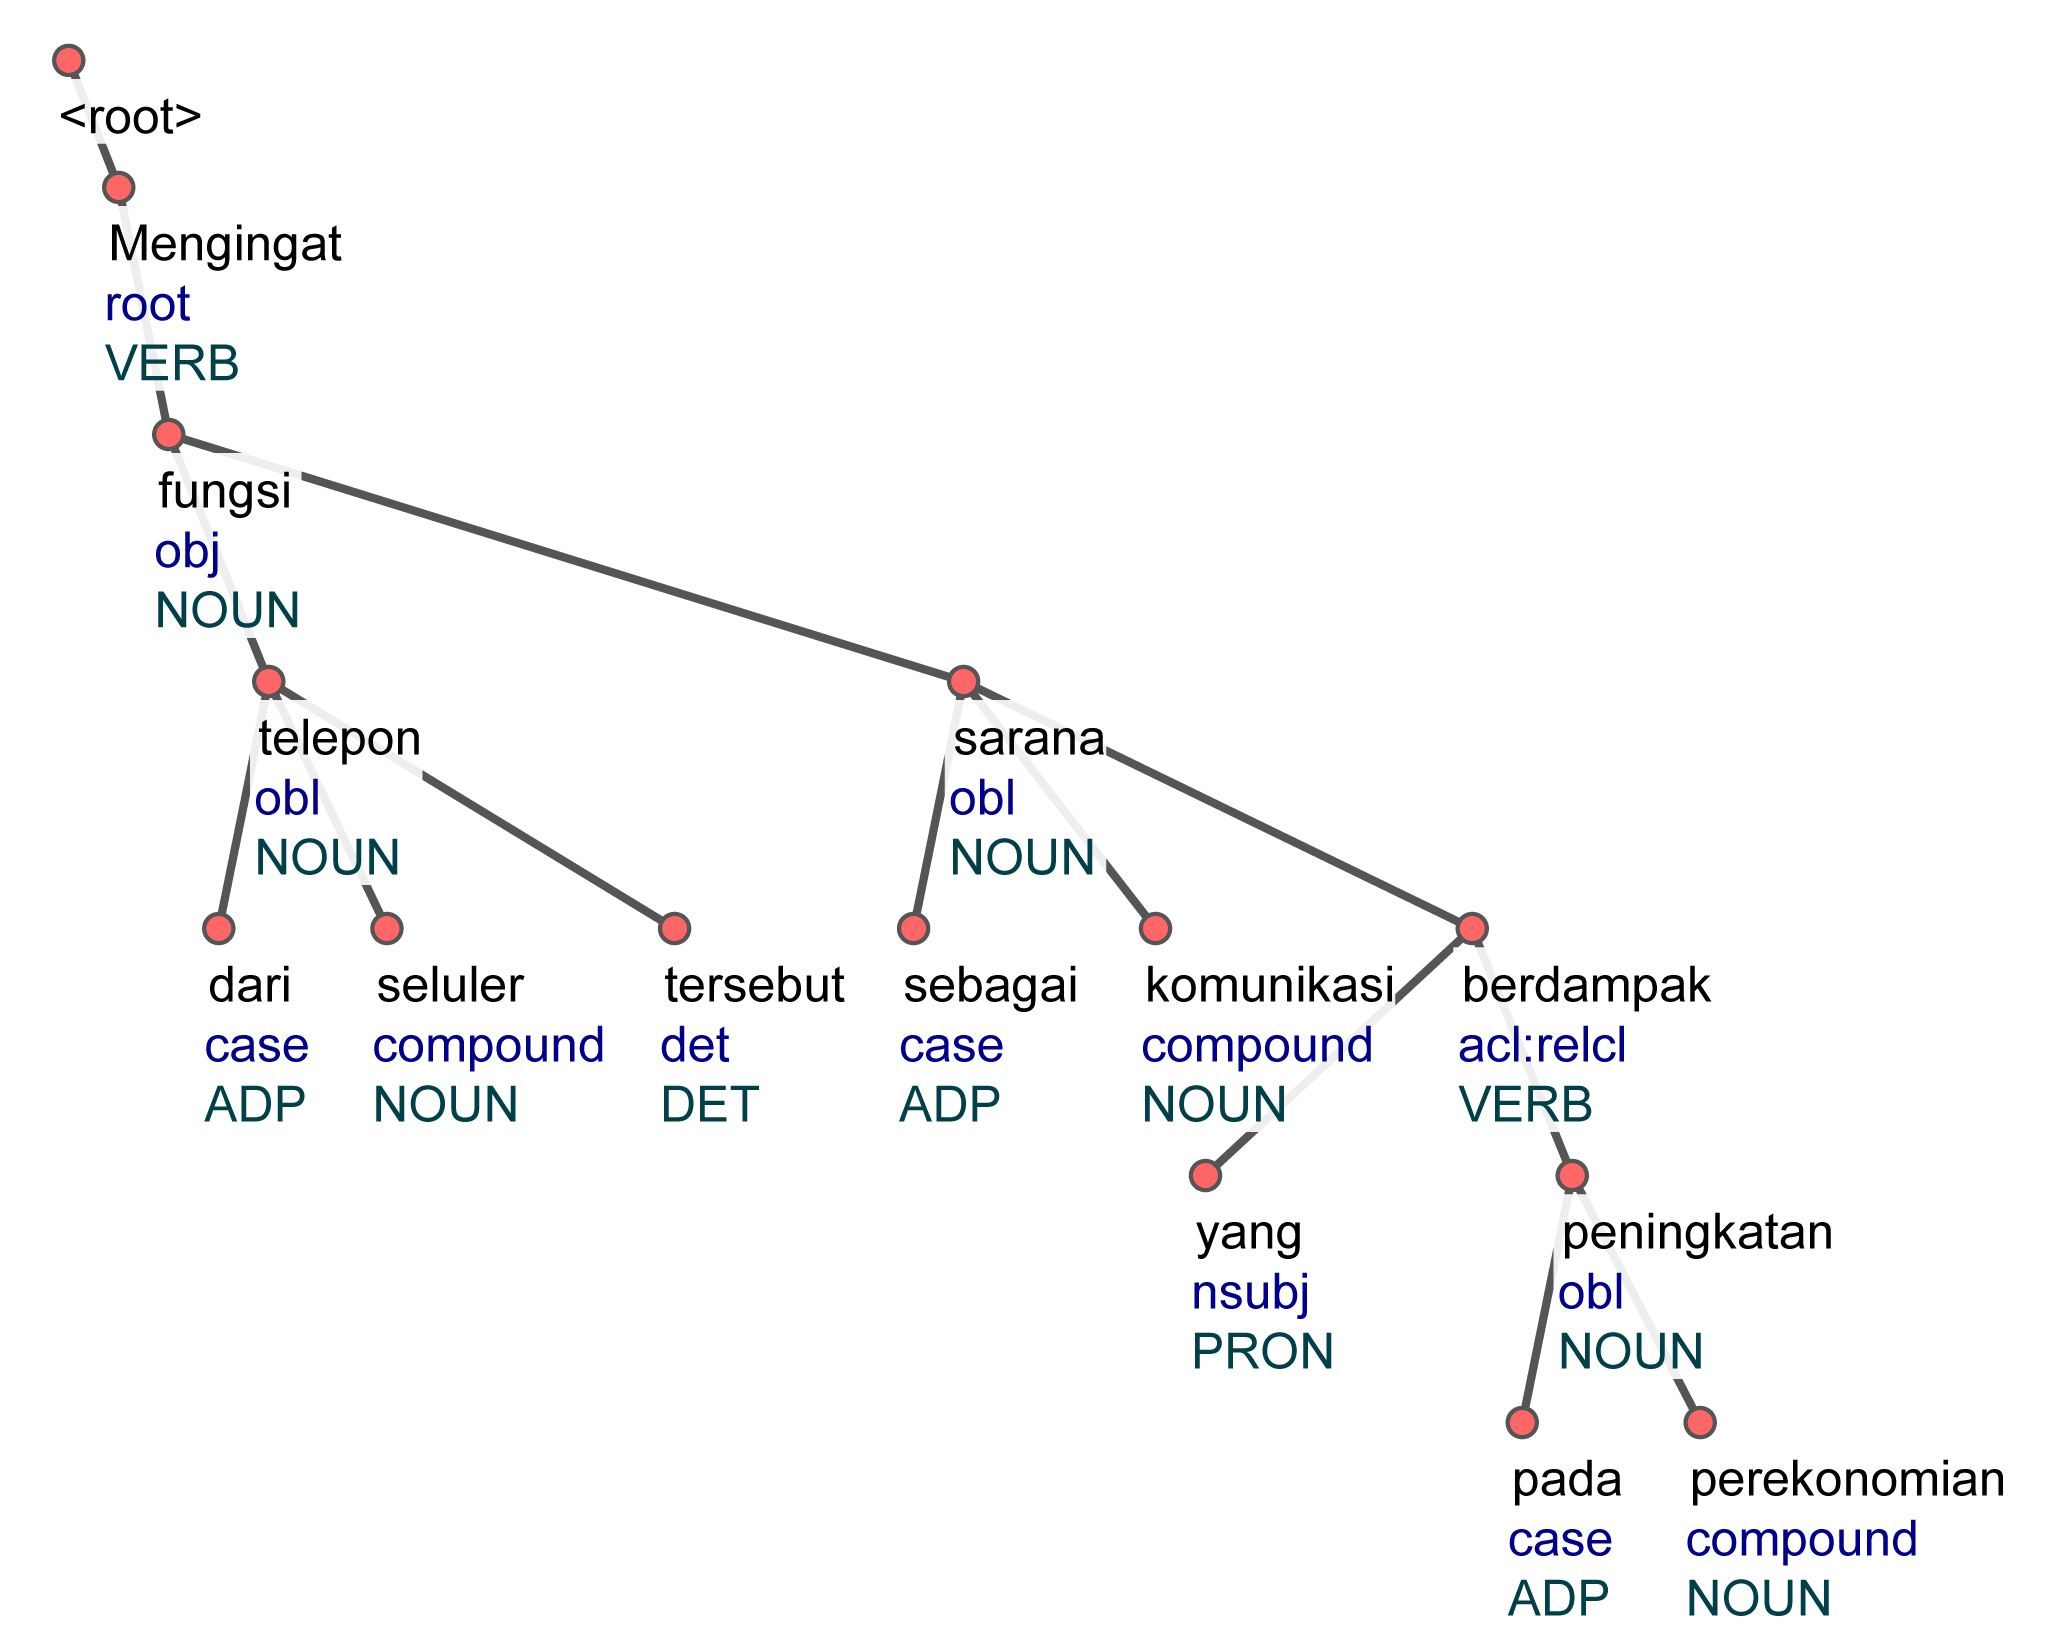
\includegraphics[width=0.8
	\textwidth] {pics/visualisasi_penguraian.jpg} 
	\caption{Contoh visualisasi penguraian kalimat berdasarkan dependensi} 
\label{fig:visualisasi_penguraian} \end{figure}

Untuk memudahkan langkah analisis kualitatif dan tinjauan secara lebih rinci terhadap tautan-tautan dependensi yang terbentuk pada sebuah kalimat, visualisasi seperti pada \pic~\ref{fig:visualisasi_penguraian} dilakukan secara terpisah. Proses visualisasi ini hanya dilakukan pada kalimat-kalimat yang akan dilihat lebih rinci sebagai contoh yang mewakili hasil temuan dengan bantuan kerangka kerja UDPipe \citep{udpipe2017}. Pada kalimat contoh ini, terlihat bahwa kalimat tersebut memiliki akar verbal \textit{mengingat} yang simpai pusatnya hanya terdiri dari satu tautan, yaitu \textit{mengingat fungsi} dengan hubungan tautan $obj$ atau obyek. Penelitian ini merupakan penelitian terhadap penggunaan tuturan nyata sehingga meskipun beberapa kalimat yang ditemukan terlihat seperti klausa terikat saja, atau tampak seperti kalimat yang tidak gramatikal, semua kalimat tetap dianalisis tanpa koreksi atau manipulasi.

\begin{center}
\begin{table} \caption{Penggalan anotasi panjang dan rata-rata jarak dependensi}\label{tab:dl_mdd}
\begin{tiny}
  \begin{tabulary}{1\textwidth}{| L | L | L | L | L | L | L | L |}
  \hline
type & sentence & dl & sum\textunderscore dl & dl\textunderscore positive & dl\textunderscore negative & mdd \\ \hline
tulis & Mengingat fungsi dari telepon seluler tersebut sebagai sarana komunikasi yang berdampak pada peningkatan perekonomian & 0 & 0 & 0 & 0 & 0.00 \\ \hline
tulis & Mengingat fungsi dari telepon seluler tersebut sebagai sarana komunikasi yang berdampak pada peningkatan perekonomian & 1 & 1 & 1 & 0 & 0.08 \\ \hline
tulis & Mengingat fungsi dari telepon seluler tersebut sebagai sarana komunikasi yang berdampak pada peningkatan perekonomian & -1 & 2 & 1 & -1 & 0.15 \\ \hline
tulis & Mengingat fungsi dari telepon seluler tersebut sebagai sarana komunikasi yang berdampak pada peningkatan perekonomian & 2 & 4 & 3 & -1 & 0.31 \\ \hline
tulis & Mengingat fungsi dari telepon seluler tersebut sebagai sarana komunikasi yang berdampak pada peningkatan perekonomian & 1 & 5 & 4 & -1 & 0.38 \\ \hline
tulis & Mengingat fungsi dari telepon seluler tersebut sebagai sarana komunikasi yang berdampak pada peningkatan perekonomian & 2 & 7 & 6 & -1 & 0.54 \\ \hline
tulis & Mengingat fungsi dari telepon seluler tersebut sebagai sarana komunikasi yang berdampak pada peningkatan perekonomian & -1 & 8 & 6 & -2 & 0.62 \\ \hline
tulis & Mengingat fungsi dari telepon seluler tersebut sebagai sarana komunikasi yang berdampak pada peningkatan perekonomian & 6 & 14 & 12 & -2 & 1.08 \\ \hline
tulis & Mengingat fungsi dari telepon seluler tersebut sebagai sarana komunikasi yang berdampak pada peningkatan perekonomian & 1 & 15 & 13 & -2 & 1.15 \\ \hline
tulis & Mengingat fungsi dari telepon seluler tersebut sebagai sarana komunikasi yang berdampak pada peningkatan perekonomian & -1 & 16 & 13 & -3 & 1.23 \\ \hline
tulis & Mengingat fungsi dari telepon seluler tersebut sebagai sarana komunikasi yang berdampak pada peningkatan perekonomian & 3 & 19 & 16 & -3 & 1.46 \\ \hline
tulis & Mengingat fungsi dari telepon seluler tersebut sebagai sarana komunikasi yang berdampak pada peningkatan perekonomian & -1 & 20 & 16 & -4 & 1.54 \\ \hline
tulis & Mengingat fungsi dari telepon seluler tersebut sebagai sarana komunikasi yang berdampak pada peningkatan perekonomian & 2 & 22 & 18 & -4 & 1.69 \\ \hline
tulis & Mengingat fungsi dari telepon seluler tersebut sebagai sarana komunikasi yang berdampak pada peningkatan perekonomian & 1 & 23 & 18 & -5 & 1.77 \\ \hline
  \end{tabulary}  
\end{tiny}
\end{table}
\end{center}

Tahap selanjutnya melibatkan proses anotasi yang berkaitan dengan panjang dan jarak tautan dependensi sebuah kalimat pada tabel hasil penguraian kalimat. \tab~\ref{tab:dl_mdd} merupakan tabel hasil anotasi terhadap salah satu kalimat di dalam korpus data. Anotasi ini dihasilkan melalui penghitungan DL dan MDD seperti yang dijabarkan pada Bab 2 dan rumus penghitungan yang dijabarkan pada Bab 3. DL menekankan pada total jarak-jarak dependensi yang didapatkan dari semua tautan dependensi dalam sebuah kalimat, sedangkan MDD menekankan pada rata-rata jarak dependensi antara dua konstituen dalam sebuah kalimat. Meskipun memiliki prinsip mendasar yang serupa, diduga ada perbedaan informasi yang berarti antara kedua pendekatan ini sehingga keduanya digunakan dalam penelitian ini. Penelitian ini tidak melakukan eksplorasi terhadap perbedaan pendekatan DL dan MDD ataupun menentukan pendekatan mana yang lebih optimal dalam mengilustrasikan efisiensi memori kerja melalui struktur sintaksis kalimat. Meskipun begitu, hasil penerapan kedua pendekatan dalam penelitian ini dapat berkontribusi dalam menunjukkan pada kondisi mana kedua pendekatan tersebut berbeda.

\tab~\ref{tab:dl_mdd} memperlihatkan penghitungan DL dan MDD untuk kalimat \textit{Mengingat fungsi dari telepon seluler tersebut sebagai sarana komunikasi yang berdampak pada peningkatan perekonomian}. Dengan jumlah konstituen 14, kalimat ini memiliki DL sejauh 23 dan MDD sejauh 1,77 konstituen. Hasil ini menunjukkan total jarak dari tautan-tautan dependensi (total Jarak Dependensi atau DD antarkonstituen) dalam kalimat tersebut berjumlah 23 dengan rata-rata jarak dependensi antara dua konstituen yang memiliki jarak tautan langsung sejauh 1,77 konstituen. Pada tabel tersebut terlihat bahwa DL juga dipisahkan menjadi dua berdasarkan direksionalitas induknya. DL positif menggambarkan kondisi relasi diawali induk yang berarti  akar atau induk direalisasikan sebelum konstituen terikat. Sebaliknya, DL negatif menggambarkan kondisi relasi diakhiri induk yang berarti akar atau induk direalisasikan setelah konstituen terikat. Analisis hubungan DL positif dan negatif ini memiliki dua bagian. Bagian pertama adalah tinjauan terhadap tautan antara dua konstituen yang memiliki tautan langsung tanpa memperhitungkan konteks frasa, klausa, atau kalimat tempat kedua konstituen tesebut berada. Analisis bagian kedua adalah tinjauan terhadap tautan antara dua konstituen di mana salah satu konstituen tersebut adalah akar verbal (simpai pusat) dan semua simpai cabang konstituen tersebut dianggap mengikuti induknya. Pada kalimat kompleks yang memiliki lebih dari satu klausa, tautan dependensi utama ini dapat membawa satu klausa atau lebih di dalamnya. Sebagai contoh, jika terdapat satu tautan dependensi utama yang negatif, dan dalam simpai cabang tersebut terdapat dua klausa, kedua klausa tersebut harus disimpan di dalam memori kerja terlebih dahulu hingga akar direalisasikan. Oleh sebab itu, posisi simpai cabang menentukan bagaimana seluruh informasi yang dikandungnya diproses. Analisis ini berangkat dari asumsi bahwa bahasa Indonesia cenderung memilih bentuk relasi diawali induk yang diambil dari indikasi dari teori struktur frasa yang mengungkapkan banyaknya kondisi di mana kata kepala akan mendahului konstituen terikatnya (\citealp{kridalaksana2002struktur, sneddon2010indonesian}).

\begin{figure}
	\centering 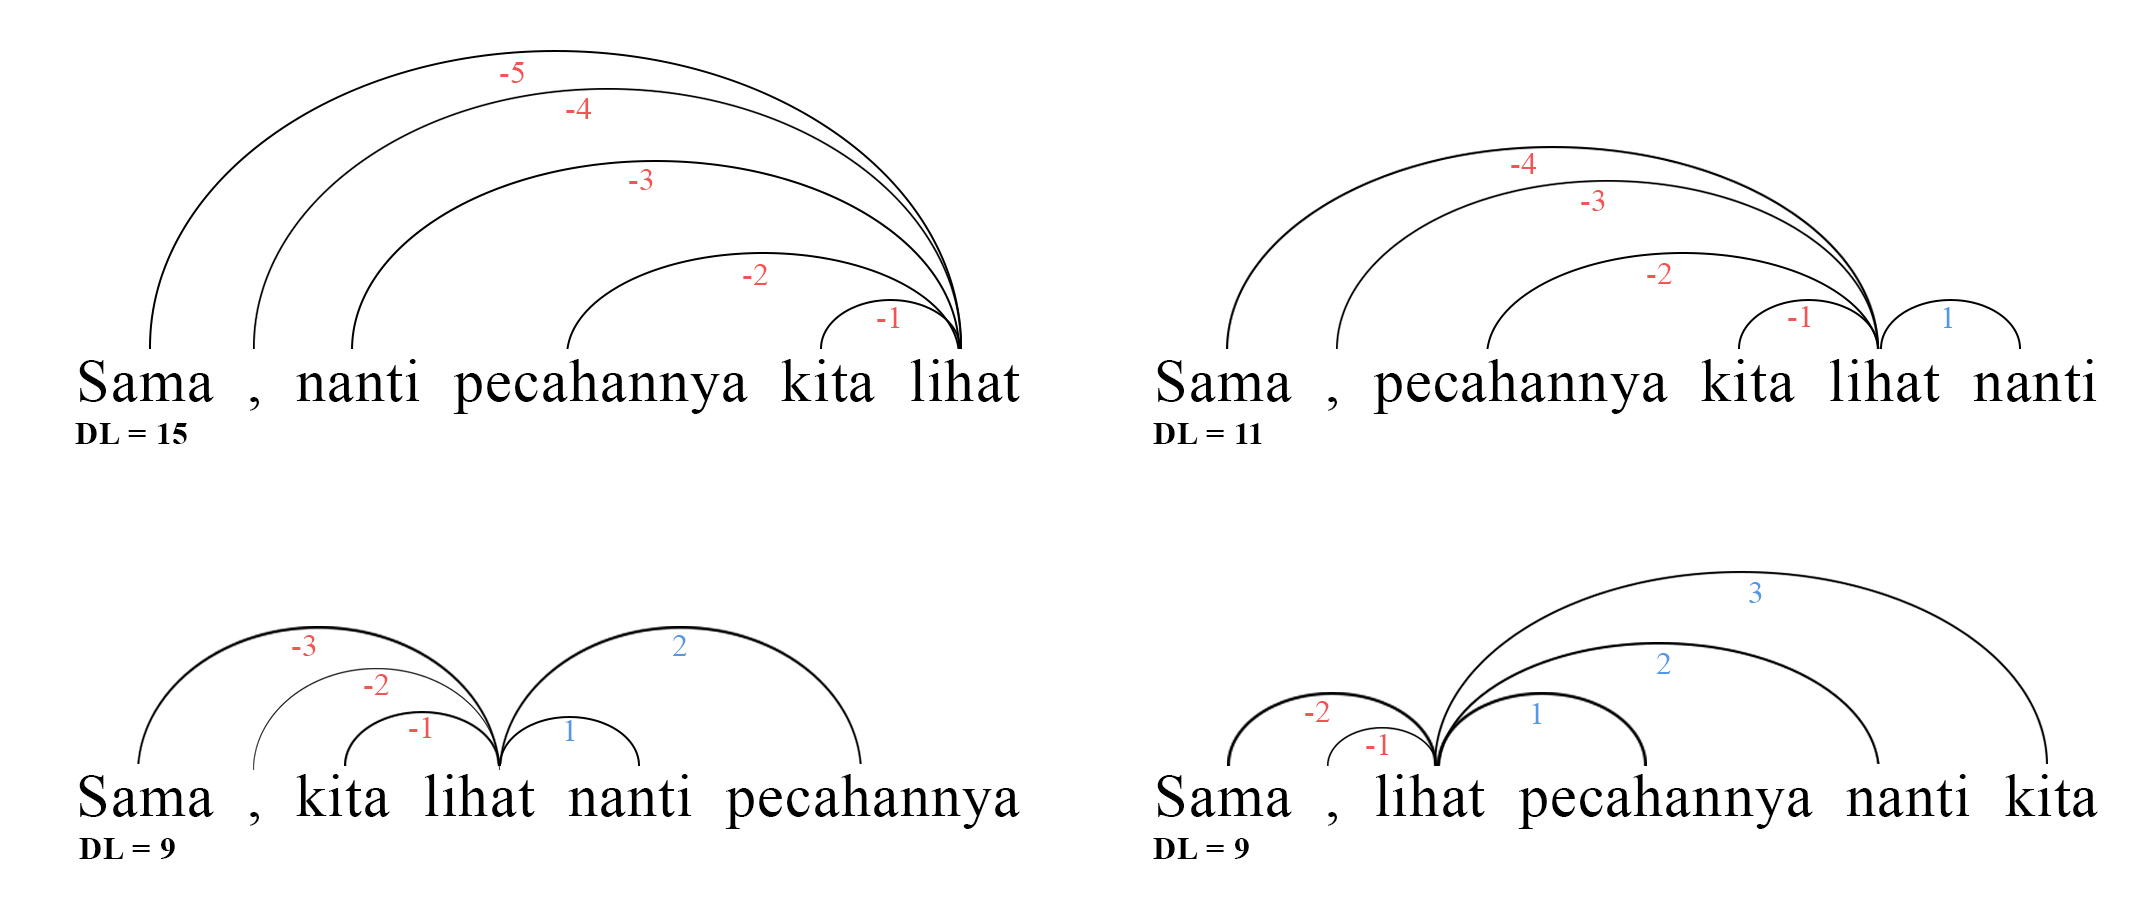
\includegraphics[width=0.8
	\textwidth] {pics/percobaan_acak.jpg} 
	\caption{Contoh hasil percobaan acak} 
\label{fig:percobaan_acak} 
\end{figure}

Berikutnya, langkah yang dilakukan setelah mendapatkan tabel hasil penguraian ini adalah percobaan acak dengan mengadopsi prinsip langkah-langkah algoritma acak \textit{Free Word Order Baseline} \citep{futrell2015large}. \textit{Free Word Order Baseline} merupakan pendekatan yang dilakukan \cite{futrell2015large} dalam menguji hipotesis adanya Pengurangan Panjang Dependensi (DLM). Pada tahap ini tidak dilakukan perbandingan untuk menguji hipotesis Pengurangan Jarak Dependensi (DDM) karena variabel pembagi, yang dalam hal ini adalah jumlah tautan, tidak berubah sehingga akan menghasilkan gambaran yang serupa dengan tinjauan terhadap DLM. Dari kalimat-kalimat yang telah diurai, percobaan ini menghasilkan 100 kombinasi struktur kalimat dengan mempertahankan kaidah tautan dependensi sesuai hasil observasi. \pic~\ref{fig:percobaan_acak} memperlihatkan tiga contoh hasil percobaan acak terhadap kalimat \textit{Sama, nanti pecahannya kita lihat} serta perbedaan DL yang didapatkan tiga kombinasi struktur lainnya. Percobaan acak ini dilakukan terhadap semua kalimat yang berada pada kategori jumlah konstituen dengan frekuensi terbanyak. Berdasarkan klasifikasi kalimat terhadap kedua korpus data dan tahap pertama analisis, frekuensi jumlah konstituen terbanyak pada setiap klasifikasi kalimat adalah 10 konstituen (ragam tulis) dan 5 konstituen (ragam lisan) untuk klasifikasi kalimat pendek (\textless= 10 konstituen), 14 konstituen (ragam tulis) dan 12 konstituen (ragam lisan) untuk klasifikasi kalimat menengah (11-20 konstituen), serta 21 konstituen (ragam tulis) dan 22 konstituen (ragam lisan) untuk klasifikasi kalimat panjang (\textgreater 20 konstituen). 

Merujuk pada penjelasan dalam tinjauan pustaka pada Bab 2, bahasa Indonesia memiliki urutan kata yang cenderung bebas, dan beberapa kasus menunjukkan pertukaran kata maupun klausa tidak mengubah makna kalimat \citep{sneddon2010indonesian}. Dalam penelitiannya, \cite{futrell2015large} menunjukkan kedekatan hasil data observasi bahasa Indonesia dengan DL minimum dengan menggunakan pendekatan ini berdasarkan korpus data yang berisi artikel penelitian. Temuan ini memberikan indikasi bahwa penerapan kebebasan urutan kata tidak hanya terjadi pada kalimat yang dianggap gramatikal, tetapi terutama pada tuturan nyata dalam kehidupan sehari-hari (data penampilan bahasa). Kebebasan terhadap aturan ini dan asumsi bahwa penutur bahasa Indonesia memanfaatkan kebebasan ini merupakan dasar utama pemilihan pendekatan \textit{Free Word Order Baseline}. Hal ini dikarenakan pendekatan tersebut menghasilkan hasil kombinasi struktur kalimat dengan panjang paling minimal dan maksimal sehingga sangat menarik untuk melihat posisi tuturan nyata yang didapat melalui observasi terhadap kemungkinan-kemungkinan kombinasi struktur yang terbentuk. 

Tahap terakhir dari analisis penelitian ini merupakan analisis kualitatif untuk melihat perilaku valensi konstituen yang difokuskan pada valensi akar verbal pada simpai pusat kalimat. Verba sebagai akar kalimat ditemukan sebanyak 84,61\% atau sebanyak 7874 kalimat pada data ragam tulis dan 70,91\% atau sebanyak 7239 kalimat pada data ragam lisan. Oleh sebab itu, bentuk ini merupakan bentuk kalimat dalam kedua korpus data. Analisis ini dilakukan untuk melihat adanya strategi yang menyebabkan terjadinya DLM dan DDM pada tingkat dependensi paling utama (simpai pusat) serta perbedaan karakter yang mungkin muncul antara kedua jenis ragam bahasa. Analisis kualitatif juga dilakukan pada temuan yang didapat pada tahap-tahap sebelumnya untuk menguraikan struktur kalimat yang mungkin memberikan informasi lebih mengenai kecenderungan penutur dalam membentuk kalimat yang efisien dari segi dependensi.

%-----------------------------------------------------------------------------%
\section{Panjang dependensi kalimat dan rata-rata jarak dependensi antarkonstituen data ragam tulis dan lisan}
%-----------------------------------------------------------------------------%
Pada bagian analisis penelitian ini, kedua pendekatan untuk menghitung DL dan MDD digunakan karena diduga masing-masing memberikan informasi yang berbeda atau menunjukkan perbedaan karakter pada kondisi tertentu. Kedua penghitungan ini dilakukan terhadap setiap kalimat dalam korpus data jurnalistik ragam lisan dan tulis. Secara garis besar, ada perbedaan yang cukup jelas terlihat dalam kedua paparan grafik nilai DL dan nilai MDD antara korpus data ragam tulis dan data ragam lisan.

%-----------------------------------------------------------------------------%
\subsection{Perbandingan panjang dependensi kalimat data ragam tulis dan lisan}
%-----------------------------------------------------------------------------%

Pada pendekatan penghitungan panjang dependensi kalimat (DL) yang diadopsi dari penelitian \cite{futrell2015large}, seluruh nilai tautan dependensi dalam sebuah kalimat dijumlahkan sehingga DL yang dihasilkan cukup sensitif dan berbanding linear dengan jumlah konstituen dalam kalimat. Pada \pic~\ref{fig:lisantulis_DL}, sumbu $x$ merepresentasikan panjang kalimat atau jumlah konstituen dan sumbu $y$ merepresentasikan DL dalam sebuah kalimat. Berdasarkan grafik ini, dapat dicermati bahwa terjadi perubahan pada kedua garis regresi antara ragam tulis dan lisan. Perbandingan umum ini dilakukan tanpa melihat lebih dalam persebaran data terkait jumlah konstituen dalam kalimat atau tanpa memperhitungkan klasifikasi panjang kalimat. Berdasarkan grafik DL ini, terlihat bahwa mayoritas jumlah konstituen dalam kalimat pada kedua korpus data berada di bawah 40 konstituen. Pada area di bawah 40 konstituen, garis regresi data ragam tulis berada di bawah garis regresi data ragam lisan. Namun, pada area di atas 40 konstituen, garis regresi menunjukkan perbandingan terbalik secara drastis. Secara umum, rata-rata DL adalah 42,61 untuk data ragam tulis dan 24,36 untuk data ragam lisan. 

\begin{figure}
	\centering 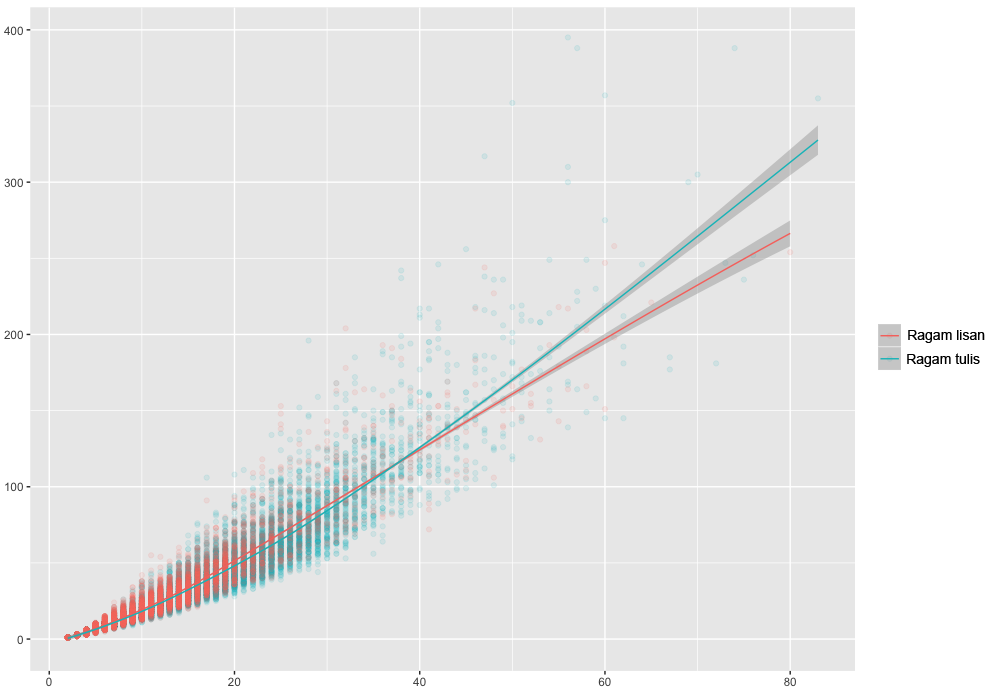
\includegraphics[width=1
	\textwidth] {pics/lisantulis_DL.png} 
	\caption{Grafik panjang dependensi data ragam tulis dan lisan} 
\label{fig:lisantulis_DL} 
\end{figure}

Tanpa memperhitungkan klasifikasi panjang kalimat, hasil rata-rata DL pada \pic~\ref{fig:lisantulis_DL} menunjukkan adanya perbedaan yang signifikan bahwa ragam lisan akan menghasilkan jumlah nilai tautan dependensi yang lebih kecil. Seperti yang terlihat pada garis regresi yang terbentuk, hingga panjang kalimat 40 konstituen, garis regresi data ragam tulis terus berada di bawah garis regresi ragam lisan dan terjadi pemusatan data pada panjang kalimat yang mendekati minimum untuk data ragam lisan. Hal ini berarti hal lain yang mempengaruhi panjang dependensi sehingga data ragam lisan dapat menghasilkan rata-rata yang lebih kecil dibandingkan data ragam tulis dilihat dari segi total panjang dependensi dalam sebuah kalimat. Hal ini menunjukkan bahwa dugaan awal ini harus dicermati lebih dalam dengan melihat klasifikasi panjang kalimat yang mungkin akan memberikan informasi tambahan lain dalam menentukan keakuratan hasil tinjauan. 

%-----------------------------------------------------------------------------%
\subsection{Perbandingan rata-rata jarak dependensi antarkonstituen data ragam tulis dan lisan}
%-----------------------------------------------------------------------------%

Berbeda dengan penghitungan DL, rata-rata jarak dependensi antarkonstituen (MDD) didapatkan dengan membagi total panjang dependensi dalam sebuah kalimat dengan jumlah tautan itu sendiri. Penghitungan ini menghasilkan perkiraan rata-rata jarak dependensi sebuah tautan dalam kalimat tersebut sehingga menggambarkan pada umumnya sejauh apa jarak relasi semantik antar dua konstituen. Seperti \pic~\ref{fig:lisantulis_DL}, \pic~\ref{fig:lisantulis_MDD} merupakan paparan MDD untuk semua kalimat pada kedua korpus data (ragam tulis dan lisan). MDD, seperti yang dikemukakan oleh \cite{liu2017dependency}, tidak terlalu sensitif terhadap jumlah konstituen karena merupakan rata-rata jarak per tautan dependensi. Meskipun begitu, berdasarkan grafik MDD ini, pada data dengan jumlah konstituen di bawah 10, MDD masih menunjukkan hasil yang sangat linear terhadap jumlah konstituen. Hal ini mengindikasikan bahwa pada jumlah konstituen yang sedikit, MDD masih memiliki tingkat sensitivitas yang cukup tinggi terhadap panjang kalimat.

\begin{figure}
	\centering 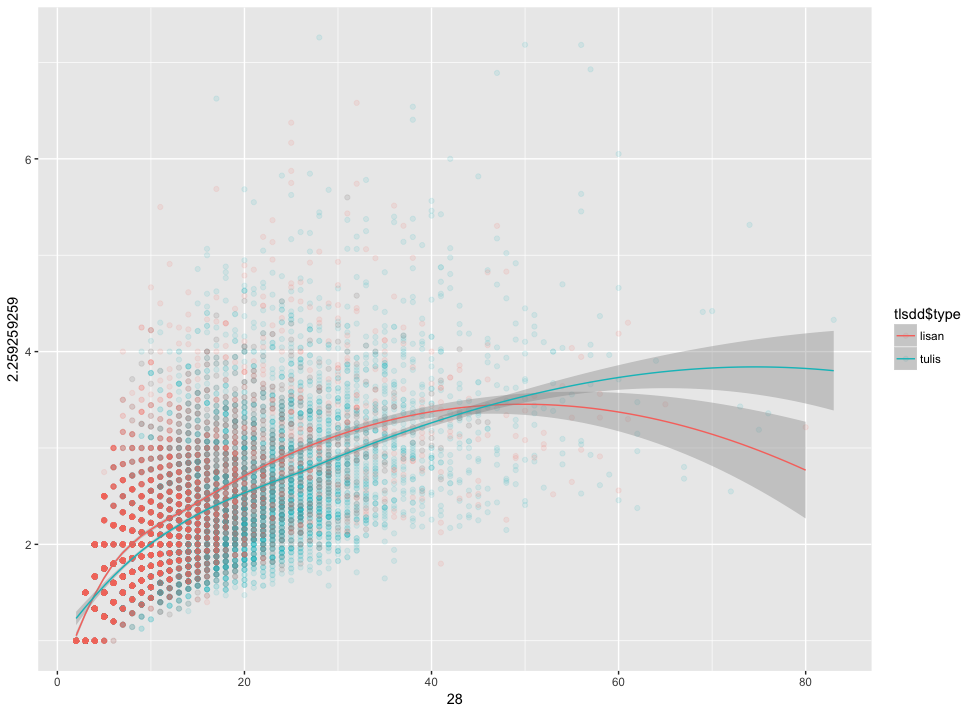
\includegraphics[width=1
	\textwidth] {pics/lisantulis_MDD.png} 
	\caption{Grafik rata-rata jarak dependensi data ragam tulis dan lisan} 
\label{fig:lisantulis_MDD} 
\end{figure}

Apabila DL memberikan gambaran umum mengenai kompleksitas sebuah kalimat karena hanya difokuskan terhadap total panjang dependensi keseluruhan kalimat, MDD dapat lebih memberikan ilustrasi kerja kognisi manusia yang tercermin pada relasi dua buah konstituen dengan kondisi agar kedua konstituen dapat bermakna secara utuh, salah satu harus menunggu yang lain untuk direalisasikan. Pada \pic~\ref{fig:lisantulis_MDD}, dapat disimpulkan bahwa garis regresi untuk korpus data ragam tulis juga berada di bawah garis regresi korpus data ragam lisan dengan panjang kalimat di bawah 40 konstituen namun berbanding terbalik setelah 40 konstituen. Temuan ini menunjukkan konsistensi antara DL dan MDD yang sama-sama menunjukkan bahwa hingga jumlah setidaknya 40 konstituen, kalimat-kalimat dalam data ragam tulis menunjukkan efisiensi yang lebih tinggi dari segi dependensi dibandingkan data ragam lisan. Namun, rata-rata MDD yang didapat dari seluruh kalimat justru memperlihatkan hasil sebaliknya. Rata-rata MDD untuk data ragam lisan adalah 2,05 konstituen dan 2,35 konstituen untuk data ragam tulis. Seperti pada catatan grafik nilai DL sebelumnya, rata-rata ini tidak memperhitungkan klasifikasi panjang kalimat dan pemusatan data ragam tulis pada panjang kalimat yang mendekati minimum yang juga patut diperhitungkan.

%%-----------------------------------------------------------------------------%
\section{Perbandingan data hasil observasi dengan hasil percobaan acak}
%%-----------------------------------------------------------------------------%
Setelah mendapatkan gambaran umum mengenai DL dan MDD untuk kedua korpus data, percobaan acak terhadap kedua korpus data dilakukan untuk melihat apakah kalimat-kalimat dalam data hasil observasi, baik ragam tulis maupun lisan, memiliki kecenderungan untuk menghindari panjang dependensi dan jarak tautan dependensi yang lebih jauh. Berdasarkan hipotesis DLM, \cite{futrell2015large} mengajukan bahwa jika bahasa berevolusi untuk mendukung komunikasi yang lebih mudah, seharusnya urutan kata yang dimanfaatkan penutur dalam tuturan nyata tidak menghasilkan panjang dependensi yang jauh. Hal ini terjadi karena panjang dependensi yang jauh mencerminkan kompleksitas produksi ataupun pemahaman yang lebih tinggi. Percobaan acak dengan pendekatan \textit{Free Word Order Baseline} menghasilkan 100 bentuk urutan konstituen acak untuk setiap kalimat dengan mempertahankan struktur tautan-tautan dependensi yang sama dengan kalimat dalam data observasi. 

Beberapa histogram berikut menunjukkan perbandingan antara DL dari semua kalimat dalam data hasil observasi dengan DL dari hasil percobaan acak dalam data ragam tulis (\pic~\ref{fig:trandomobs}) serta ragam lisan (\pic~\ref{fig:lrandomobs}). Sumbu $x$ menandakan panjang dependensi dan sumbu $y$ menandakan persentase jumlah kalimat yang memiliki DL tersebut. Perbandingan ini dilakukan dengan mengontrol jumlah konstituen sehingga hasil percobaan acak dapat memberikan nilai yang spesifik. \cite{futrell2015large} pernah menampilkan histogram serupa dengan jumlah konstituen sebanyak 12. Berdasarkan penelitiannya, nilai terkecil dari data bahasa Indonesia hasil observasi sangat mendekati nilai minimum dari hasil percobaan acak.

\begin{figure}
\centering

\begin{subfigure}{.45\textwidth}
  \centering
  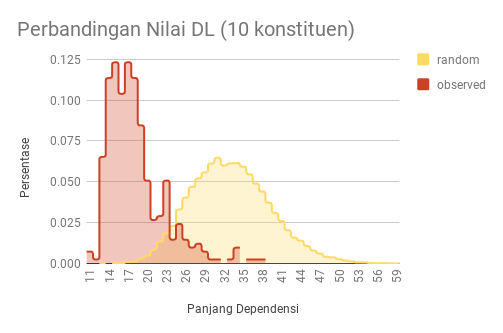
\includegraphics[width=1\linewidth]{pics/t10randomobs.png}
  \caption{10 konstituen}
  \label{fig:t10randomobs} 
\end{subfigure}
%
\begin{subfigure}{.45\textwidth}
  \centering
  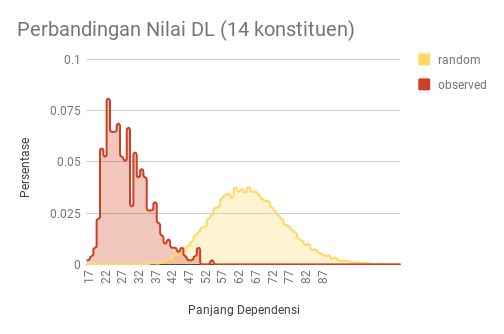
\includegraphics[width=1\linewidth]{pics/t14randomobs.png}
  \caption{14 konstituen}
  \label{fig:t14randomobs} 
\end{subfigure}
%
\begin{subfigure}{.45\textwidth}
  \centering
  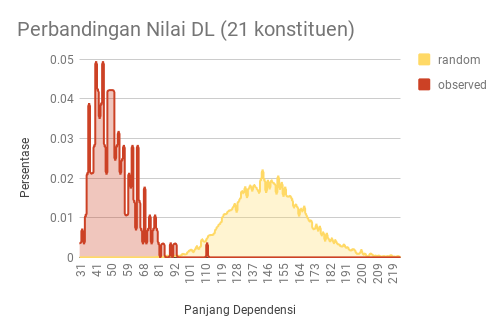
\includegraphics[width=1\linewidth]{pics/t21randomobs.png}
  \caption{21 konstituen}
  \label{fig:t21randomobs} 
\end{subfigure}

\caption{Panjang dependensi data hasil observasi dan hasil percobaan acak untuk panjang kalimat 10,14, dan 21 konstituen pada data ragam tulis}
\label{fig:trandomobs}
\end{figure}

\pic~\ref{fig:trandomobs} memperlihatkan histogram perbandingan DL antara data hasil observasi dengan hasil percobaan acak untuk jumlah konstituen 10, 14, dan 21. Jumlah-jumlah konstituen ini memiliki frekuensi terbanyak yang mewakili setiap kelompok klasifikasi kalimat pada data ragam tulis.  Histogram hasil percobaan acak terlihat jelas membentuk kurva yang lebih rendah dibandingkan dengan kurva yang dibentuk oleh data observasi. Hal ini berarti hasil percobaan acak memiliki distribusi DL yang lebih besar dibandingkan dengan data observasi. Berdasarkan histogram ini, dapat dilihat juga bahwa pada jumlah konstituen yang semakin banyak, irisan antara kurva nilai DL data observasi dan hasil percobaan acak semakin sedikit.

\begin{table}
\begin{center}
\begin{small}
  \caption{Tabel perbandingan rata-rata panjang dependensi data hasil observasi dan hasil percobaan acak untuk data ragam tulis}  \label{tab:perbandingan_DL_tulis}
  \begin{tabular}{ | l | l | l | l |}
    \hline
    	Jumlah konstituen & Rata-rata nilai DL (observasi) & Rata-rata nilai DL (acak) & p-value \\ \hline
	10 & \textbf{18,14} & 33,01 & \textless 0,001 \\ \hline
	14 & \textbf{29,11} & 64,95 & \textless 0,001 \\ \hline
	21 & \textbf{51,59} & 146,67 & \textless 0,001 \\ \hline
  \end{tabular}
  \end{small}
\end{center}
\end{table}

\tab~\ref{tab:perbandingan_DL_tulis} menunjukkan perbedaan rata-rata DL yang cukup jauh antara data hasil observasi dengan hasil percobaan acak untuk data ragam tulis dengan efek yang signifikan pada semua jumlah konstituen (\textit{P} \textless 0,001). Semua histogram dan perbedaan rata-rata tersebut mengkonfirmasi terjadinya DLM pada data hasil observasi ragam tulis sehingga kalimat-kalimat pada korpus tersebut lebih efisien dibandingkan dengan hasil percobaan acaknya.

\begin{figure}
\centering

\begin{subfigure}{.45\textwidth}
  \centering
  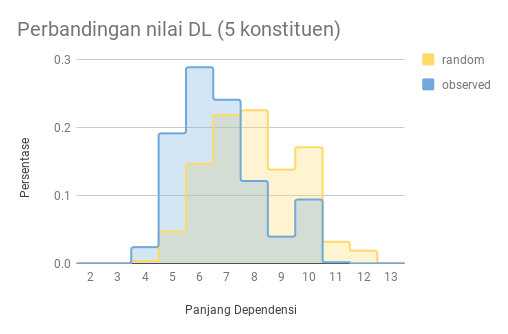
\includegraphics[width=1\linewidth]{pics/l5randomobs.png}
  \caption{5 konstituen}
  \label{fig:l5randomobs} 
\end{subfigure}
%
\begin{subfigure}{.45\textwidth}
  \centering
  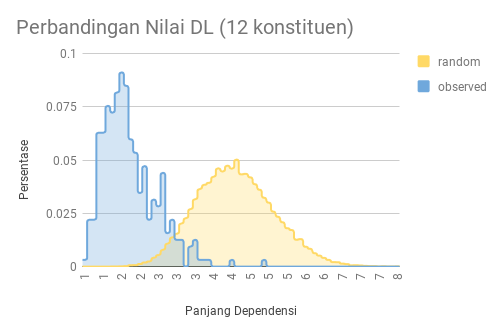
\includegraphics[width=1\linewidth]{pics/l12randomobs.png}
  \caption{12 konstituen}
  \label{fig:l12randomobs} 
\end{subfigure}
%
\begin{subfigure}{.45\textwidth}
  \centering
  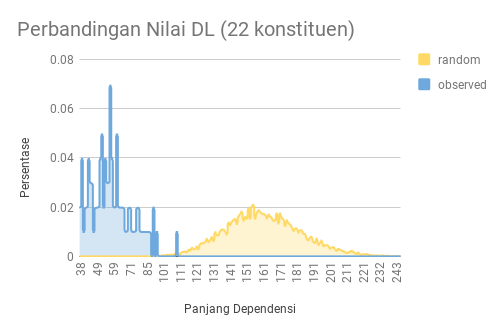
\includegraphics[width=1\linewidth]{pics/l22randomobs.png}
  \caption{22 konstituen}
  \label{fig:l22randomobs} 
\end{subfigure}

\caption{Panjang dependensi data hasil observasi dan hasil percobaan acak untuk panjang kalimat 5,12, dan 22 konstituen pada data ragam lisan}
\label{fig:lrandomobs}
\end{figure}

Sesuai dengan ekspektasi, percobaan acak terhadap data ragam lisan menunjukkan hasil yang serupa dengan percobaan terhadap data ragam tulis. \pic~\ref{fig:lrandomobs} merupakan histogram perbandingan DL antara data hasil observasi dengan hasil percobaan acak untuk jumlah konstituen 5, 12, dan 22 yang mewakili setiap kelompok klasifikasi kalimat pada data ragam lisan. Histogram hasil percobaan acak untuk ragam lisan juga membentuk kurva yang secara jelas terlihat lebih rendah dan juga menandakan bahwa  acak memiliki distribusi DL yang lebih besar dibandingkan dengan data hasil observasi. Bahkan untuk jumlah konstituen 5 yang tergolong kalimat sangat pendek, data observasi masih memperlihatkan adanya indikasi DLM secara signifikan dengan nilai \textit{P} \textless 0,001. Berdasarkan histogram ini juga dapat dilihat bahwa pada jumlah konstituen yang semakin banyak, irisan antara nilai DL data observasi dan hasil percobaan acak semakin sedikit. Hal ini berarti DLM semakin jelas terlihat pada kalimat yang semakin panjang.

\begin{table}
\begin{center}
\begin{small}
  \caption{Tabel perbandingan rata-rata panjang dependensi data hasil observasi dan hasil percobaan acak untuk data ragam lisan}  \label{tab:perbandingan_DL_lisan}
  \begin{tabular}{ | l | l | l | l |}
    \hline
	 Jumlah konstituen & Rata-rata nilai DL (observasi) & Rata-rata nilai DL (acak) & \textit{p-value} \\ \hline
	 5 & \textbf{6,74} & 7,98 & \textless 0,001 \\ \hline
	 12 & \textbf{24,78} & 47,7 & \textless 0,001 \\ \hline
	 22 & \textbf{58,92} & 160,89 & \textless 0,001 \\ \hline
  \end{tabular}
  \end{small}
\end{center}
\end{table}

Serupa juga dengan percobaan terhadap data ragam tulis, \tab~\ref{tab:perbandingan_DL_lisan} menunjukkan perbedaan rata-rata DL yang cukup jauh antara data hasil observasi dan hasil percobaan acak untuk data ragam lisan dengan efek yang signifikan pada semua jumlah konstituen (\textit{P} \textless 0,001). Berdasarkan semua paparan tersebut, dapat disimpulkan juga bahwa kalimat-kalimat pada data hasil observasi ragam lisan juga lebih efisien dibandingkan hasil percobaan acaknya.

Percobaan acak pada kedua korpus data dengan jumlah konstituen yang berbeda-beda menunjukkan adanya optimasi struktur kalimat pada data hasil observasi sehingga terjadi pengurangan panjang dependensi (DLM) secara menyeluruh. Histogram hasil percobaan acak menunjukkan bahwa pada semua jumlah konstituen, distribusi DL data hasil observasi jauh lebih padat dan mendekati jumlah minimum. Temuan ini sejalan dengan hipotesis penelitian \cite{hawkins2014cross} yang menyebutkan bahwa aturan urutan kata mendasar yang dalam pemahaman penutur akan menghasilkan konstruksi kalimat yang tautan dependensinya lebih pendek dibandingkan alternatif konstruksi yang mungkin ada.

Hipotesis pengurangan panjang atau jarak dependensi (DLM atau DDM) berbicara tentang kecenderungan manusia untuk mendekatkan kata-kata yang memiliki relasi semantik. Pendekatan ini dapat dilakukan dengan menerapkan beberapa strategi seperti yang telah dibahas pada penelitian-penelitian terdahulu (\citealp{jaeger2006redundancy, gildea2015human}). Dalam ranah sintaksis, strategi pendekatan-kata-kata ini termasuk melalui penyusunan urutan kata dan pengurangan kata dalam kalimat (yang mungkin diakibatkan oleh pengurangan unsur yang repetitif ataupun hal yang lain). Berdasarkan tahap pertama analisis, yaitu percobaan acak dengan menggunakan \textit{Free Word Order Baseline} \citep{futrell2015large}, dihasilkan 100 kemungkinan struktur kalimat yang tidak memiliki aturan urutan kata tertentu. Percobaan ini mendukung hipotesis bahwa terjadi DLM pada kedua korpus data (ragam tulis maupun ragam lisan) secara signifikan (\textit{P} \textless 0,001). 

Temuan DLM ini juga berkaitan dengan pengurangan jarak dependensi (DDM) karena percobaan acak tidak mengubah jumlah konstituen dalam kalimat yang sama sehingga variabel pembagi DL sebuah kalimat tidak berubah. Temuan ini menandakan bahwa struktur kalimat-kalimat dalam data hasil observasi pada kedua ragam memperlihatkan struktur yang lebih optimal dari segi dependensi dalam menghasilkan DL yang lebih pendek dibandingkan kemungkinan struktur lain yang terbentuk. Perlu ditekankan bahwa struktur yang optimal ini dinilai dari segi dependensi dan bukan dari segi tata bahasa. Hal ini berarti terlepas dari standar gramatikal dan keberterimaannya, variasi struktur kalimat yang ada dalam kedua korpus rata-rata cukup mengoptimalkan memori kerja dan mengindikasikan kemudahan untuk berkomunikasi. Penentuan apakah sebuah struktur optimal, gramatikal, serta mudah dipahami berada di luar batasan penelitian ini. Metodologi lain seperti uji persepsi perlu dilakukan untuk mendapatkan temuan yang akurat. Penilaian dan pengukuran struktur yang lebih optimal dari segi produksi maupun pemahaman berada di luar batasan penelitian ini, sehingga perlu diadakan penelitian lebih lanjut yang melibatkan metodologi transdisipliner dengan ilmu kognitif serta uji persepsi.

%%-----------------------------------------------------------------------------%
\section{Persebaran kalimat dan kaitannya terhadap panjang dependensi kalimat dan rata-rata jarak dependensi antarkonstituen}
%%-----------------------------------------------------------------------------%

Pada \pic~\ref{fig:lisantulis_DL}  dan \pic~\ref{fig:lisantulis_MDD} dalam pembahasan sebelumnya, terlihat jelas adanya perbedaan persebaran kalimat pada kedua korpus data terkait dengan panjang kalimat atau jumlah konstituen. Gambaran umum yang didapatkan dan garis regresi yang ditunjukkan pada kedua gambar tersebut menimbulkan pertanyaan yang hanya dapat dijawab melalui analisis dengan memperhitungkan panjang kalimatnya. Berdasarkan korpus data yang terkumpul, persebaran kalimat pada kedua ragam berbeda secara signifikan. 

\begin{table}
\begin{center}
\begin{small}
   \caption{Persentase kalimat pada tabel klasifikasi jumlah konstituen}  \label{tab:presentase_kalimat}
  \begin{tabular}{ |p{3cm} | p{3cm} | p{3cm} | p{3cm} |}
    \hline
 & Kalimat pendek \newline (\textless=10 konstituen) & Kalimat menengah (11-20 konstituen) & Kalimat panjang (\textgreater20 konstituen) \\ \hline
Data Ragam Tulis & 23,33\% & 45,54\% & 31,13\% \\ \hline
Data Ragam Lisan & 59,49\% & 29,16\% & 11,35\% \\ \hline
  \end{tabular}
  \end{small}
\end{center}
\end{table}

Pada data ragam tulis, sebanyak 45,54\% kalimat berada pada klasifikasi kalimat menengah (\tab~\ref{tab:presentase_kalimat}). Klasifikasi kalimat pendek dan panjang pada ragam tulis memiliki jumlah kalimat yang tidak jauh berbeda. Sementara itu, sebanyak 59,49\% kalimat pada data ragam lisan berada pada klasifikasi kalimat pendek dan menurun secara drastis pada klasifikasi kalimat menengah dan panjang.  

\begin{figure}
	\centering 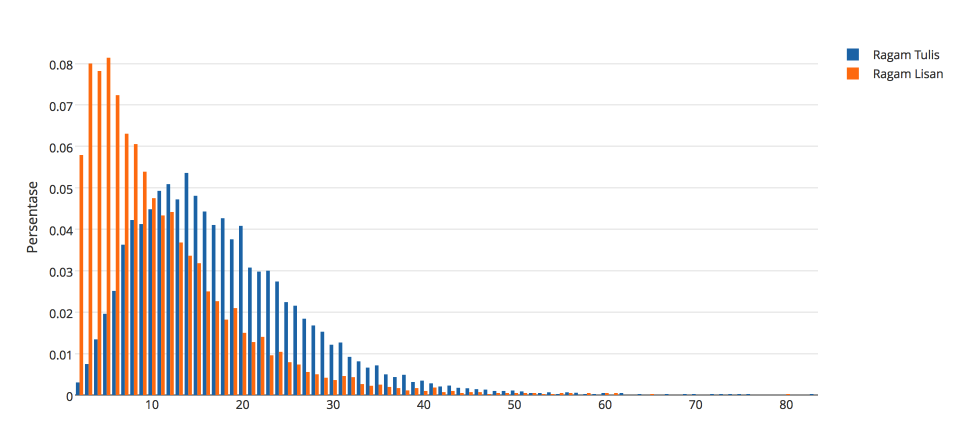
\includegraphics[width=1
	\textwidth] {pics/Jumlah_kata.png} 
	\caption{Diagram perbandingan jumlah konstituen data ragam tulis dan lisan} 
	\label{fig:jumlah_kata} 
\end{figure}

Seperti yang terlihat pada \pic~\ref{fig:jumlah_kata}, terdapat kepadatan yang sangat tinggi pada panjang kalimat di bawah 10 konstituen untuk data ragam lisan, sementara kepadatan tertinggi pada data ragam lisan terletak pada kalimat dengan panjang menengah. Hal ini memperlihatkan bahwa persebaran panjang kalimat pada kedua korpus tidak boleh dihiraukan dalam menganalisis kaitannya dengan panjang dan jarak dependensi. Panjang kalimat dengan frekuensi terbanyak pada data ragam tulis adalah 14 konstituen. Sementara itu, frekuensi terbanyak yang ditemukan pada ragam lisan adalah panjang kalimat 5 konstituen.

%%-----------------------------------------------------------------------------%
\subsection{Pemusatan data ragam lisan pada klasifikasi kalimat pendek (\textless= 10 konstituen)}
%%-----------------------------------------------------------------------------%
Pemusatan data pada klasifikasi kalimat pendek (\textless= 10 konstituen) pada data ragam lisan cukup besar hingga melebihi 50\% dari total jumlah kalimat dalam korpus tersebut. Hal ini berdampak pada perbandingan rata-rata DL serta MDD antara data ragam tulis dan lisan pada kelompok klasifikasi tersebut (\tab~\ref{tab:DL_MDD_pendek}).

\begin{table}
\begin{center}
\begin{small}
\caption{Perbandingan rata-rata panjang dan rata-rata jarak dependensi pada klasifikasi kalimat pendek }\label{tab:DL_MDD_pendek}
  \begin{tabular}{ | p{3.2cm} | p{3.2cm} | p{3.2cm} | p{2cm} |}
    \hline
 & Kalimat pendek \newline (\textless =10 konstituen) \newline Data ragam tulis & Kalimat pendek \newline (\textless =10 konstituen) \newline Data ragam lisan & \textit{p-value} \\ \hline
 Rata-rata nilai DL & 11,85 & \textbf{8,76} & \textless 0,001 \\ \hline
 Rata-rata nilai MDD & 1,792 & \textbf{1,687} & \textless 0,001 \\ \hline
 Rata-rata jumlah konstituen & 7,356 & \textbf{5,708} & \textless 0,001 \\ \hline
 Jumlah kalimat & 2220 & 6073 & -- \\ \hline
   \end{tabular}
   \end{small}
\end{center}
\end{table}

Berdasarkan \tab~\ref{tab:DL_MDD_pendek}, DL dan MDD data ragam lisan lebih pendek dibandingkan data ragam tulis pada klasifikasi kalimat pendek secara signifikan. Berbeda dengan \pic~\ref{fig:lisantulis_DL}  dan \pic~\ref{fig:lisantulis_MDD} yang tidak memperhitungkan klasifikasi panjang kalimat, terutama karena DL berkorelasi cukup linear terhadap panjang kalimat, rata-rata DL pada data ragam lisan dalam klasifikasi ini adalah 8,76. Hasil ini lebih pendek dibandingkan dengan hasil yang didapatkan dari data ragam tulis karena pemusatan jumlah konstituen yang mendekati minimum pada data ragam lisan akan mempengaruhi hasil yang didapat. Hal ini dapat dilihat dari perbandingan rata-rata jumlah konstituen dan jumlah kalimat yang muncul pada klasifikasi ini dengan perbedaan yang signifikan. Meskipun jumlah kalimat data ragam lisan pada klasifikasi ini jauh lebih banyak, rata-rata jumlah konstituen dalam satu kalimat lebih sedikit dibandingkan data ragam tulis.  Berkaitan dengan pemusatan data tersebut, rata-rata MDD data ragam lisan juga menjadi lebih pendek dibandingkan data ragam tulis. Temuan ini menunjukkan indikasi bahwa penggunaan kalimat pendek menjadi salah satu preferensi (dan mungkin strategi)  untuk meningkatkan efisiensi kalimat dalam percakapan lisan. Dalam beberapa kasus di korpus data ragam lisan, ditemukan kalimat-kalimat yang sebenarnya merupakan klausa terikat yang berdiri sendiri sebagai sebuah kalimat utuh dan lepas dari klausa utama yang mungkin berada pada kalimat-kalimat sebelumnya. Seperti contoh, kalimat-kalimat ini banyak ditemukan ditandai dengan konjungsi \textit{dan} pada posisi pertama. 

\begin{table}
\begin{center}
\begin{small}
\caption{Perbandingan panjang dependensi kalimat dengan panjang kurang dan lebih dari 5 konstituen pada klasifikasi kalimat pendek}\label{tab:DL_5}
  \begin{tabular}{ | p{3.2cm} | p{3.2cm} | p{3.2cm} | p{2cm} |}
    \hline
Jumlah konstituen & Data ragam tulis & Data ragam lisan & \textit{p-value} \\ \hline
\textless= 5 konstituen & 4,54 & \textbf{3,92} & \textless 0,001 \\ \hline
6-10 konstituen & 13,75 & 13,6 & \textgreater 0,05 \\ \hline
   \end{tabular}
   \end{small}
\end{center}
\end{table}

\begin{table}
\begin{center}
\begin{small}
\caption{Perbandingan rata-rata jarak dependensi kalimat dengan panjang kurang dan lebih dari 5 konstituen pada klasifikasi kalimat pendek}\label{tab:MDD_5}
  \begin{tabular}{ | p{3.2cm} | p{3.2cm} | p{3.2cm} | p{2cm} |}
    \hline
Rentang & Data ragam tulis & Data ragam lisan & \textit{p-value} \\ \hline
\textless= 5 konstituen & 1,443 & \textbf{1,402} & \textless 0,05 \\ \hline
6-10 konstituen & \textbf{1,883} & 1,972 & \textless 0,001 \\ \hline
   \end{tabular}
   \end{small}
\end{center}
\end{table}

Kepadatan data ragam lisan yang sangat tinggi pada klasifikasi ini memunculkan analisis tambahan untuk melihat perbandingan yang terjadi di dalam klasifikasi ini. Sebelumnya, \cite{wang2017effects} menemukan bahwa MDD ragam teks yang lebih formal lebih kecil dibandingkan ragam teks yang ditujukan untuk ujaran lisan mulai dari panjang kalimat sebanyak 6 konstituen. Dari temuan ini, analisis tambahan dilakukan untuk meninjau perbandingan DL dan MDD pada panjang kalimat kurang dan lebih dari 5 konstituen. \tab~\ref{tab:DL_5} memperlihatkan bahwa perbedaan yang signifikan terkait total panjang dependensi sebuah kalimat hanya ditemukan pada klasifikasi panjang kalimat kurang dari atau sama dengan 5 konstituen. Namun, \tab~\ref{tab:MDD_5} memperlihatkan perbedaan yang signifikan terkait rata-rata jarak dependensi antara dua konstituen dalam kalimat pada kedua sub-klasifikasi, namun berbanding terbalik. Data ragam lisan dengan panjang kalimat kurang dari atau sama dengan 5 konstituen menunjukkan efisiensi yang lebih tinggi, tetapi mulai 6 konstituen, ragam tulis justru memperlihatkan efisiensi yang lebih tinggi dari segi jarak antara dua konstituen.

\begin{figure}
\centering

\begin{subfigure}{.3\linewidth}
  \centering
  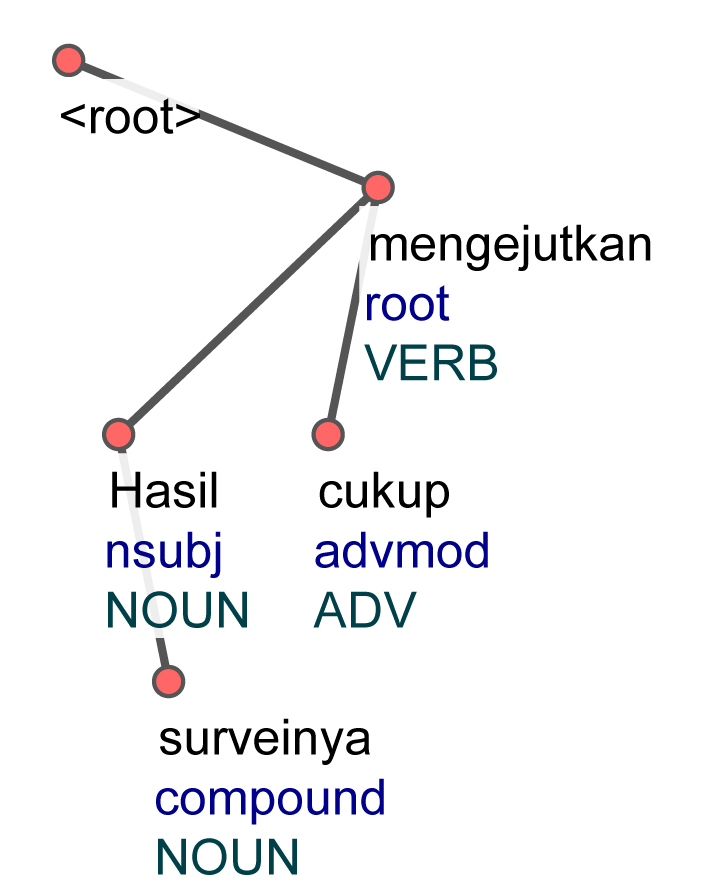
\includegraphics[width=1\linewidth] {pics/ts662.jpg} 
	\caption{T4}
	\label{fig:ts662} 
\end{subfigure}
%
\begin{subfigure}{.35\linewidth}
  \centering
  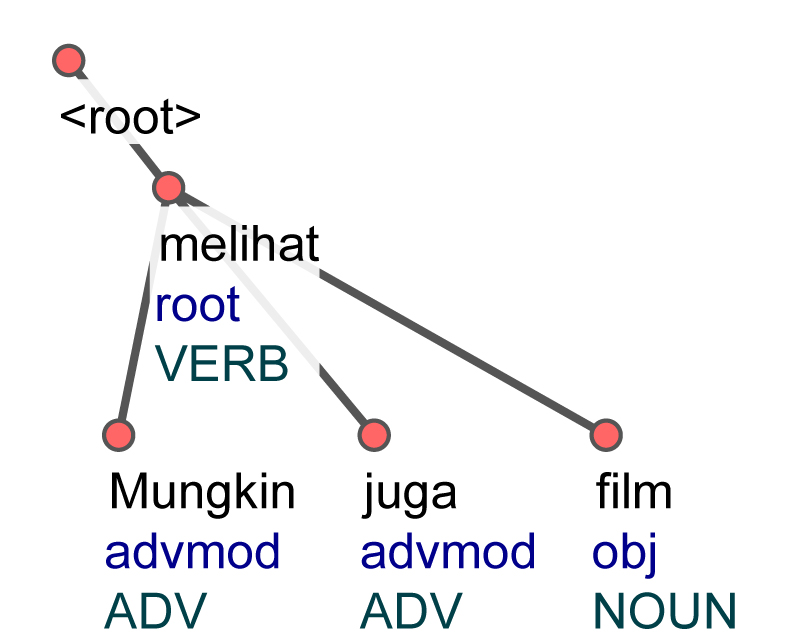
\includegraphics[width=1\linewidth]{pics/ls1102.jpg} 
	\caption{L4}
	\label{fig:ls1102} 
\end{subfigure}

\caption{Contoh perbandingan struktur sintaktis pada panjang kalimat 4 konstituen}
\label{fig:struktur4}
\end{figure}

Panjang dan jarak dependensi ditemukan signifikan pada klasifikasi kalimat pendek, terutama pada panjang kalimat kurang dari atau sama dengan 5 konstituen. Pada contoh kalimat T4 (\pic~\ref{fig:ts662}) yang diambil dari ragam tulis dan kalimat L4 (\pic~\ref{fig:ls1102}) yang diambil dari ragam lisan, perbedaan yang jelas terlihat adalah tidak adanya aktor pelaku pada kalimat L4. Tingkat atau level dependensi yang semakin ke bawah antara dua kalimat tersebut berbeda di mana tingkat kedalaman dependensi T4 lebih banyak. DL dan MDD pada kalimat T4 (\pic~\ref{fig:ts662}) adalah 5 dan 1,67, sementara pada kalimat L4 (\pic~\ref{fig:ls1102}) adalah 4 dan 1,33. Namun, karena jumlah konstituen yang sangat sedikit, perbedaan struktur sintaktis tidak terlalu signifikan secara visual sehingga kurang bisa diasumsikan bahwa ada perbedaan karakteristik yang mendasar antara kedua ragam. 

%%-----------------------------------------------------------------------------%
\subsection{Perbedaan signifikansi panjang dan rata-rata jarak dependensi pada klasifikasi kalimat menengah (11-20 konstituen)}
%%-----------------------------------------------------------------------------%
Pada kelompok klasifikasi kalimat menengah dengan panjang kalimat sebanyak 11 hingga 20 konstituen, terlihat adanya perbedaan dalam perbandingan nilai-nilai di antara kedua ragam. Pada klasifikasi ini ditemukan perbandingan terbalik antara rata-rata DL dan MDD pada kedua korpus data (\tab~\ref{tab:DL_MDD_menengah}). Untuk DL, data ragam lisan memiliki rata-rata yang sedikit lebih pendek, yaitu 33,05 dibandingkan data ragam tulis (33,32) namun perbedaan ini tidak signifikan (\textit{P} \textgreater 0,05). Hal ini berarti perbedaan antara jenis ujaran tulis dan lisan tidak mempengaruhi panjang dependensi. Meskipun begitu, temuan yang menarik adalah bahwa rata-rata MDD data ragam tulis (2,31) lebih pendek dibandingkan dengan data ragam lisan (2,404) secara signifikan. Jumlah kalimat kedua korpus data tidak jauh berbeda dan selisih rata-rata jumlah konstituen juga tidak sebesar pada klasifikasi kalimat pendek, namun perbedaannya signifikan. Hal ini berarti pada klasifikasi kalimat menengah, masih terlihat kecenderungan untuk menggunakan kalimat yang lebih pendek pada ragam lisan.  

\begin{table}
\begin{center}
\begin{small}
 \caption{Perbandingan rata-rata panjang dan rata-rata jarak dependensi pada klasifikasi kalimat menengah}\label{tab:DL_MDD_menengah}  
 \begin{tabular}{| p{3.2cm} | p{3.2cm} | p{3.2cm} | p{2cm} |}
    \hline
 & Kalimat menengah \newline (11-20 konstituen) \newline Data ragam tulis & Kalimat menengah \newline (11-20 konstituen) \newline Data ragam lisan & \textit{p-value} \\ \hline
 Rata-rata nilai DL & 33,32 & 33,05 & \textgreater 0,05  \\ \hline
 Rata-rata nilai MDD & \textbf{2,31} & 2,404 & \textless 0,001 \\ \hline
 Rata-rata jumlah konstituen & 15,24 & \textbf{14,56} & \textless 0,001 \\ \hline
 Jumlah kalimat & 4210 & 2976 & -- \\ \hline
   \end{tabular}
   \end{small}
\end{center}
\end{table}

Dengan mempertimbangkan hasil pada (\tab~\ref{tab:DL_MDD_menengah}) yang menunjukkan bahwa rata-rata DL dan MDD kedua korpus data berbanding terbalik, temuan ini memperlihatkan adanya indikasi bahwa pada panjang kalimat tertentu, jumlah konstituen yang lebih sedikit tidak selalu berfungsi sebagai strategi untuk menghasilkan kalimat yang efisien dari segi dependensi. Indikasi pada kelompok klasifikasi ini menarik karena memperlihatkan bahwa meskipun total jarak yang dihasilkan semua tautan dependensi lebih kecil pada satu klasifikasi, tidak berarti menggambarkan jarak antarkonstituen yang lebih kecil juga.

%%-----------------------------------------------------------------------------%
\subsection{Tidak ada kecenderungan jumlah konstituen pada klasifikasi kalimat panjang (\textgreater20 konstituen)}
%%-----------------------------------------------------------------------------%

Berbeda dengan kedua klasifikasi panjang kalimat sebelumnya, rata-rata nilai DL dan MDD pada data ragam tulis lebih pendek dibandingkan data ragam lisan (\tab~\ref{tab:DL_MDD_panjang}) dan perbedaan ini bersifat signifikan. Hal ini berarti terlepas dari persebaran kalimatnya yang cukup banyak (31,13\%) dari keseluruhan korpus data ragam tulis, kalimat dengan jumlah konstituen yang lebih banyak pada data ragam tulis cenderung memiliki struktur yang lebih efisien dibandingkan dengan data ragam lisan. MDD data ragam tulis lebih pendek dibandingkan data ragam lisan secara signifikan mulai dari jumlah konstituen sebanyak 6 hingga klasifikasi kalimat terpanjang dan semua perbedaannya signifikan. Hal ini berarti ada kecenderungan yang konsisten mulai jumlah konstituen tersebut bahwa konstruksi kalimat pada bahasa Indonesia ragam tulis lebih efisien dari segi dependensi.

\begin{table}
\begin{center}
\begin{small}
\caption{Perbandingan rata-rata panjang dan rata-rata jarak dependensi pada klasifikasi kalimat panjang}  \label{tab:DL_MDD_panjang}
\begin{tabular}{ | p{3.2cm} | p{3.2cm} | p{3.2cm} | p{2cm} |}
    \hline
 & Kalimat panjang \newline (\textgreater20 konstituen) \newline Data ragam tulis & Kalimat panjang \newline (\textgreater20 konstituen) \newline Data ragam lisan & \textit{p-value} \\ \hline
 Rata-rata nilai DL & \textbf{79,94} & 83,84 & \textless 0,01 \\ \hline
 Rata-rata nilai MDD & \textbf{2,844} & 3,018 & \textless 0,001 \\ \hline
 Rata-rata jumlah konstituen & 28,39 & 28,36 & \textgreater 0,05 \\ \hline
 Jumlah kalimat & 2876 & 1158 & -- \\ \hline
   \end{tabular}
   \end{small}
\end{center}
\end{table}

Berdasarkan \tab~\ref{tab:DL_MDD_panjang}, jumlah kalimat antara keduanya cukup jauh berbeda. Tetapi, selisih rata-rata jumlah konstituen sangat kecil dan perbedaannya tidak signifikan. Hal ini berarti pada klasifikasi kalimat panjang berdasarkan data yang dikumpulkan, tidak ada kecenderungan atau preferensi terkait panjang kalimat terkait ragam tertentu. Signifikansi temuan ini konsisten hingga jumlah konstituen sebanyak 40 dalam arti hingga panjang kalimat tersebut, data ragam tulis menunjukkan efisiensi kalimat yang lebih tinggi dibandingkan data ragam lisan baik dari segi panjang dependensi keseluruhan kalimat maupun rata-rata jarak antara dua konstituten. Signifikansi ini melemah pada panjang kalimat di atas 40 konstituen. Hal ini mungkin disebabkan oleh persebaran jumlah kalimat kedua korpus pada rentang ini sangat sedikit dibandingkan rentang panjang kalimat yang lain.  

Untuk memberikan ilustrasi terhadap perbandingan struktur kalimat kelompok klasifikasi kalimat panjang, berikut adalah beberapa contoh kalimat dengan jumlah konstituen sebanyak 22 dan 31 yang diambil dari kedua korpus data, yaitu kalimat T22 (\pic~\ref{fig:ts3901}), T31a (\pic~\ref{fig:ts2079}) dan T31b (\pic~\ref{fig:ts2081}) yang diambil dari ragam tulis serta L22 (\pic~\ref{fig:ls6521}), , L31a (\pic~\ref{fig:ls1716}), L31b (\pic~\ref{fig:ls16}), dan L31c (\pic~\ref{fig:ls114}) yang diambil dari ragam lisan. Kelima kalimat berikut menunjukkan adanya karakter utama yang secara cukup jelas membedakan konstruksi struktur kalimat antara kedua ragam. 

\begin{figure}
	\centering 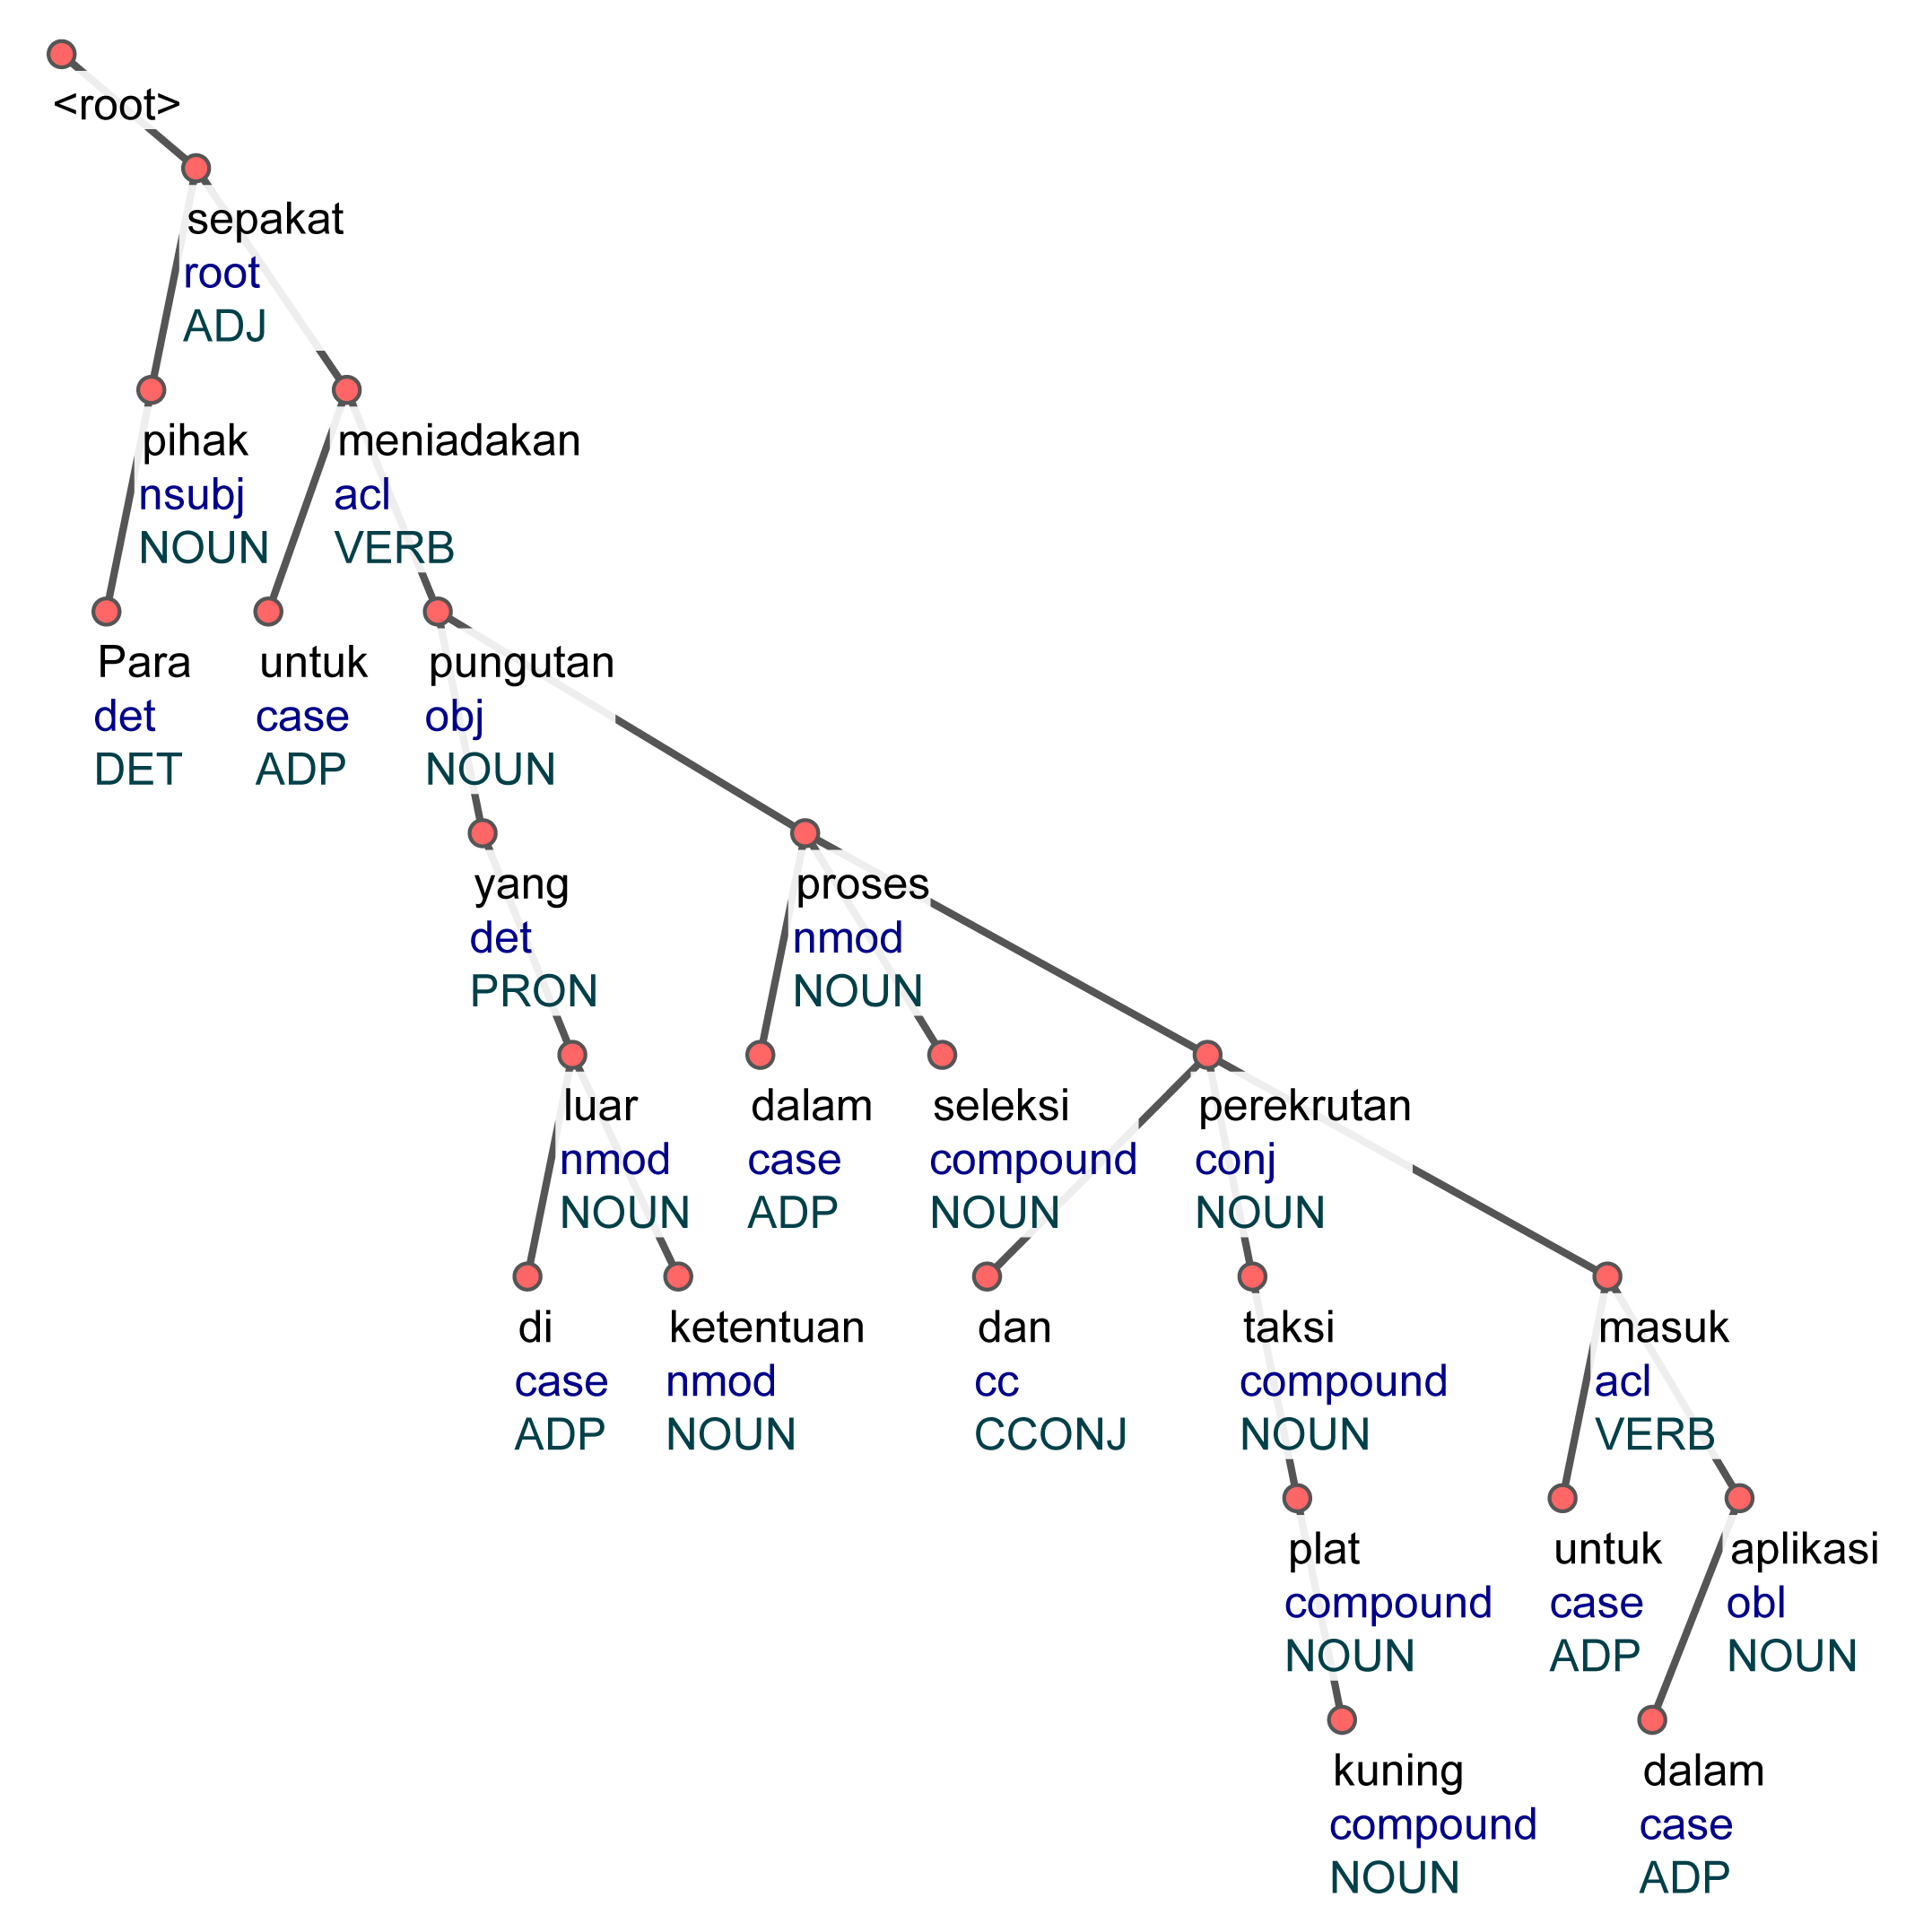
\includegraphics[width=0.8
	\textwidth] {pics/ts3901.jpg} 
	\caption{Kalimat T22 pada data ragam tulis} 
	\label{fig:ts3901} 
\end{figure}

Konstituen \textit{sepakat} pada kalimat T22 (\pic~\ref{fig:ts3901}) merupakan akar yang memiliki tautan-tautan dependensi terhadap konstituen-konstituen terikatnya. Induk pada simpai cabang terdekat pada kalimat T22 cenderung memiliki jumlah konstituen sedikit meskipun mengandung beberapa klausa terikat. Pada kalimat T22 ini terlihat banyak tautan dependensi dari dua konstituen yang berdampingan seperti pada relasi simpai-simpai antara konstituen \textit{para}, \textit{pihak}, dan \textit{sepakat}, antara konstituen \textit{meniadakan}, \textit{pungutan}, dan \textit{yang}, serta beberapa tautan lainnya. Berdasarkan bank pohon struktur dependensi ini, terlihat juga ada percabangan utama yang bersifat berlanjut antara \textit{sepakat}, \textit{meniadakan}, \textit{pungutan}, \textit{proses}, \textit{perekrutan}, dan \textit{masuk}. Relasi berlanjut ini mencerminkan adanya percabangan searah meskipun bukan terhadap dua konstituen yang berdampingan. Kalimat T22 (\pic~\ref{fig:ts3901}) memiliki DL sejauh 35 dan MDD sejauh 1,667 konstituen. Selisih antara DL dari tautan-tautan dependensi positif dan negatif sebesar 19 dalam arti jumlah tautan dengan bentuk relasi diawali induk lebih banyak dan/atau berjarak lebih jauh dibandingkan bentuk relasi yang sebaliknya.


\begin{figure}
	\centering 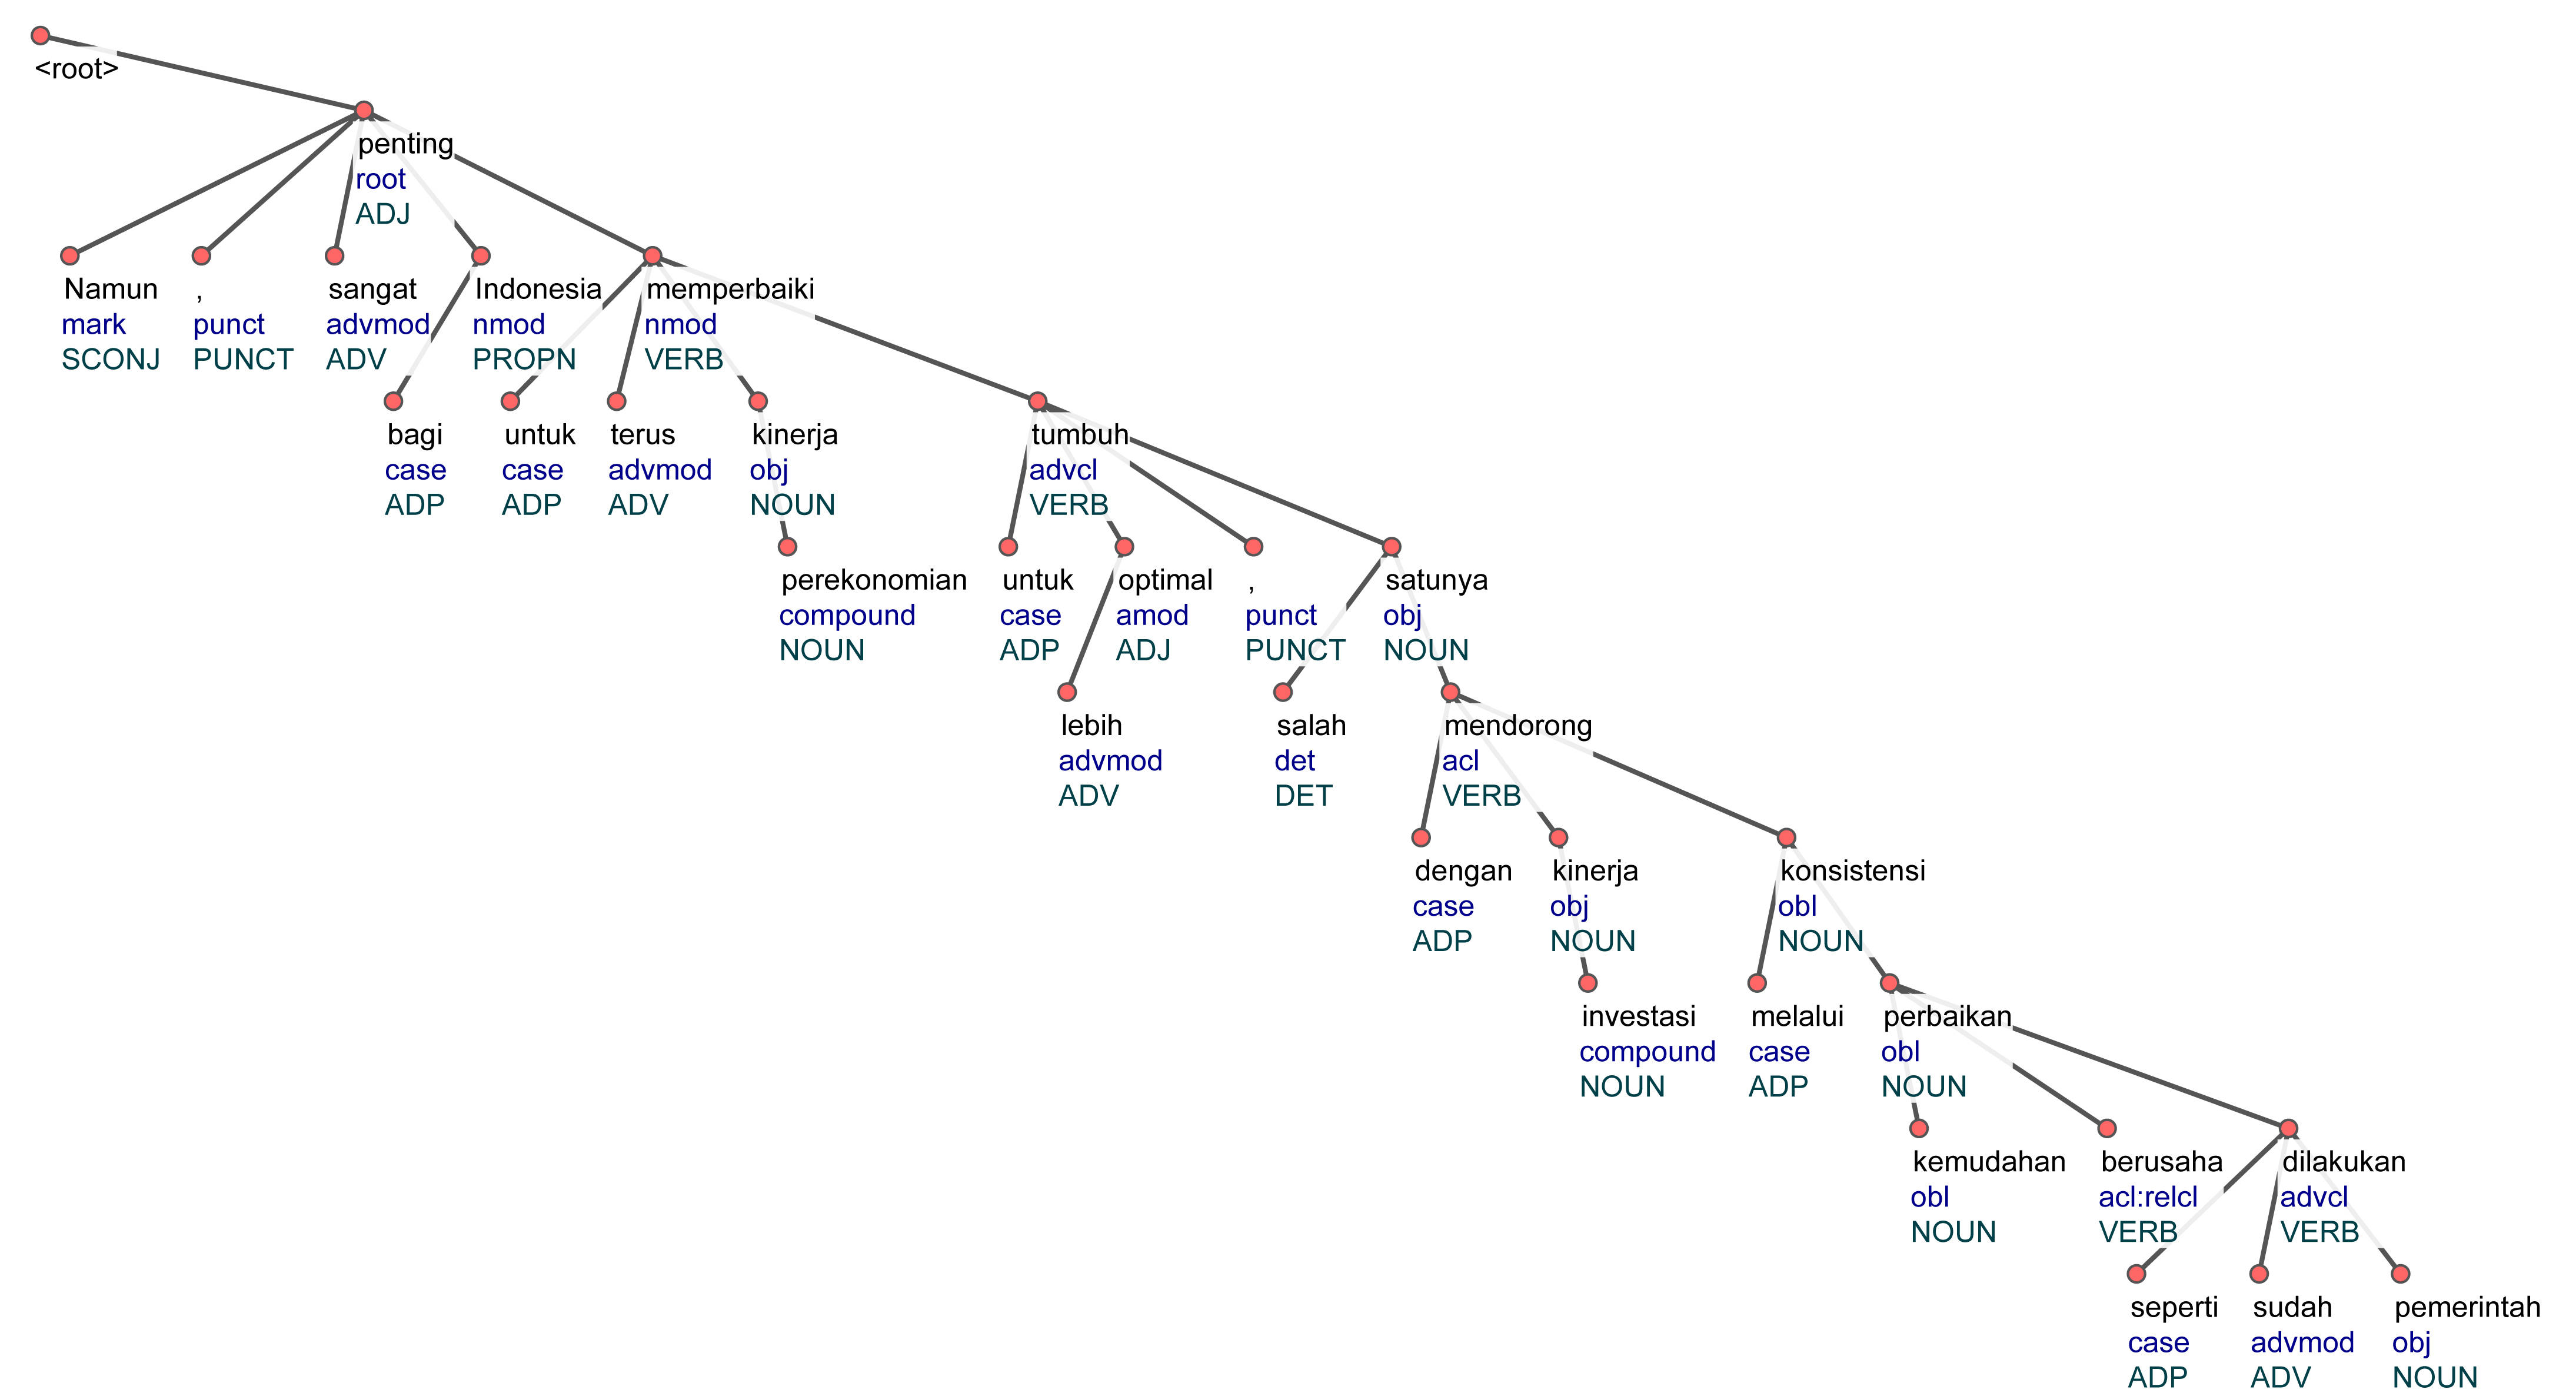
\includegraphics[width=1
	\textwidth] {pics/ts2079.jpg} 
	\caption{Kalimat T31a pada data ragam tulis} 
	\label{fig:ts2079} 
\end{figure}

Akar adjektiva \textit{penting} pada kalimat T31a (\pic~\ref{fig:ts2079}) mengikat verba \textit{memperbaiki} yang dihubungkan dengan konjungsi \textit{untuk} dalam kaidah dependensi. Induk pada simpai cabang terdekat ini juga cenderung memiliki jumlah konstituen sedikit meskipun mengandung beberapa klausa terikat. Pola ini terlihat berulang pada simpai-simpai cabang berikutnya mengakibatkan banyak simpai cabang lain yang tidak memiliki tautan langsung dengan akar dan banyak terbentuk tautan antara dua konstituen yang berdampingan. Seperti kalimat T22, relasi antara simpai-simpai konstituen \textit{penting}, \textit{memperbaiki}, \textit{kinerja}, \textit{mendorong}, \textit{konsistensi}, \textit{berusaha}, dan \textit{dilakukan} bersifat berlanjut mencerminkan adanya percabangan searah meskipun bukan terhadap dua konstituen yang berdampingan. Kalimat T31a (\pic~\ref{fig:ts2079}) memiliki DL sejauh 68 dan MDD sejauh 2,267 konstituen. Selisih antara DL dari tautan-tautan dependensi positif dan negatif sebesar 16 yang juga berarti jumlah tautan dengan bentuk relasi diawali induk lebih banyak dan/atau berjarak lebih jauh dibandingkan bentuk relasi yang sebaliknya.

\begin{figure}
	\centering 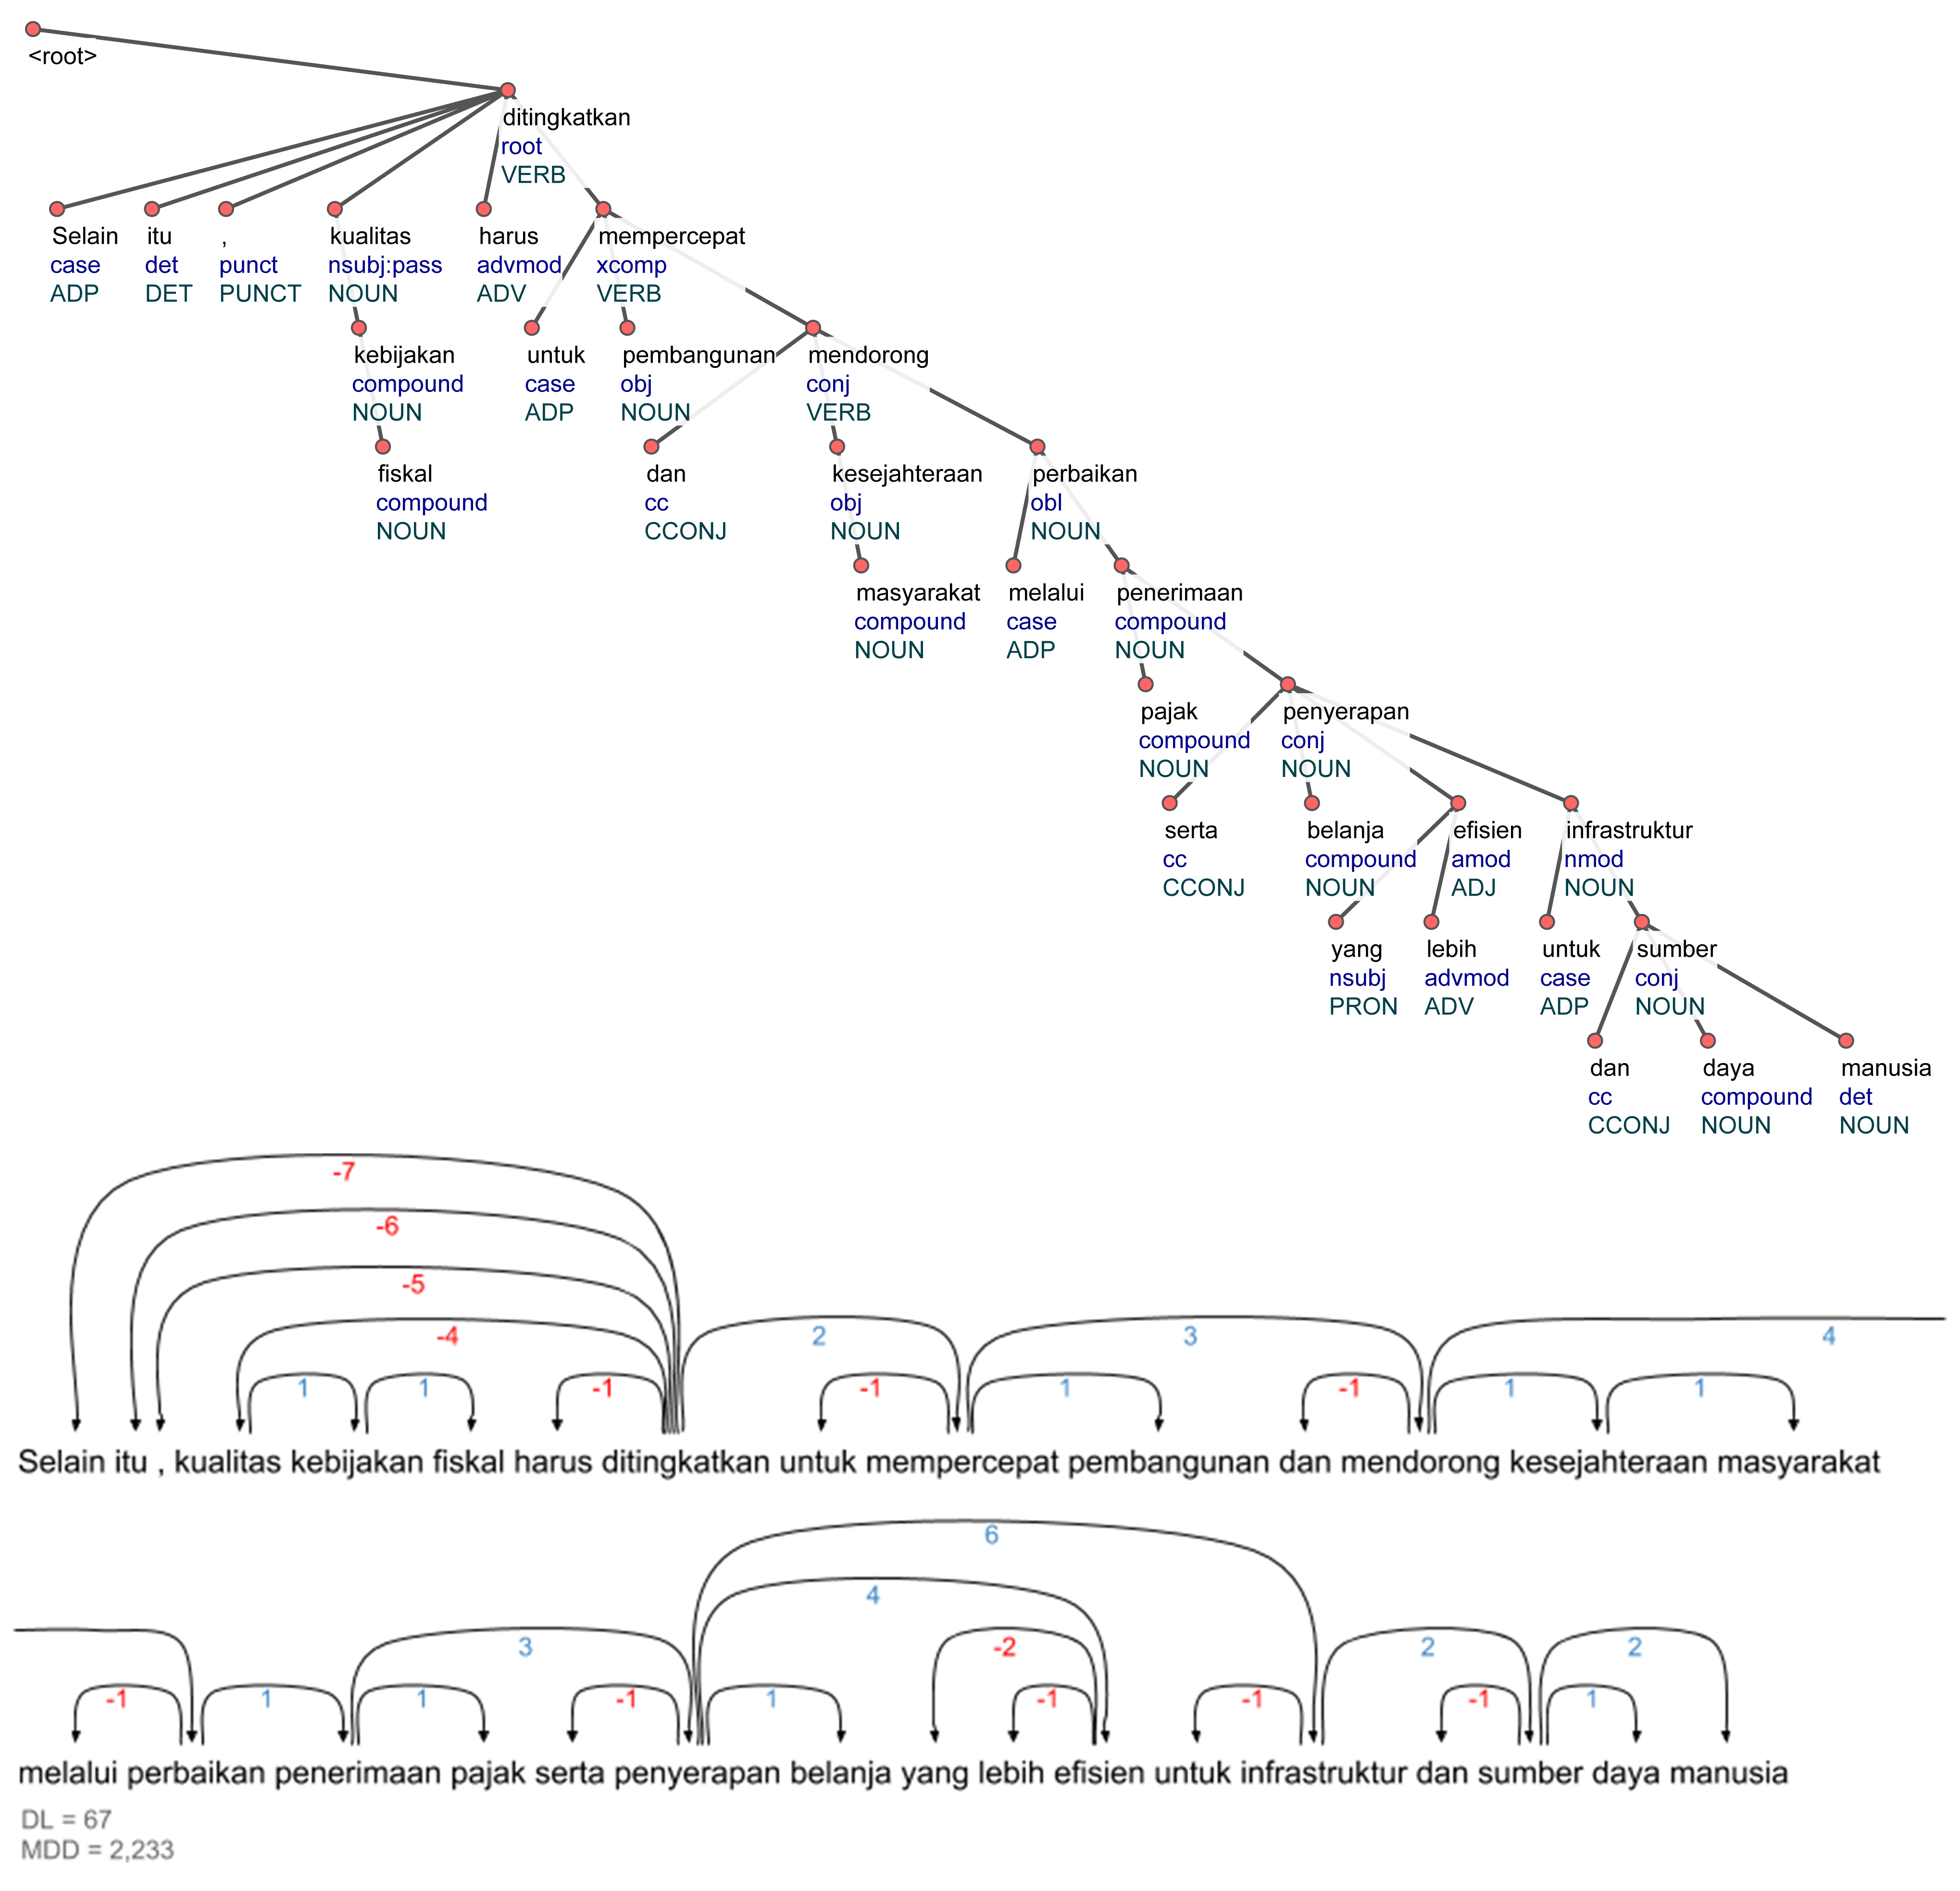
\includegraphics[width=1
	\textwidth] {pics/ts2081.jpg} 
	\caption{Kalimat T31b pada data ragam tulis} 
	\label{fig:ts2081} 
\end{figure}

Seperti kalimat T22 dan T31a, konstituen \textit{ditingkatkan} pada kalimat T31b (\pic~\ref{fig:ts2081}) juga merupakan akar yang memiliki beberapa tautan dependensi terhadap konstituen terikatnya. Pada kalimat ini, akar verbal \textit{ditingkatkan} mengikat verba lain \textit{mempercepat} yang juga dihubungkan dengan konjungsi tujuan \textit{untuk}. Juga seperti kalimat T31a, banyak simpai-simpai cabang pada kalimat T31b tidak memiliki tautan langsung dengan akar mengakibatkan adanya percabangan searah. Kalimat T31b (\pic~\ref{fig:ts2081}) memiliki DL sejauh 67 dan MDD sejauh 2,233 konstituen. Meskipun struktur kalimat T31b terlihat serupa dengan kalimat T31a dan DL serta MDD yang cukup dekat, selisih DL dari tautan-tautan dependensi positif dan negatif sangat kecil, yaitu hanya sebesar 3. Hal ini berarti jumlah bentuk relasi diawali induk dan jumlah bentuk relasi diakhiri induk dalam kalimat tersebut cukup seimbang. 

Pada ketiga kalimat, terutama kalimat T22 dan T31a, terlihat pergerakan simpai dan percabangan yang semakin menurun ke arah sesudah akar atau ke arah kanan. Percabangan menurun ke kanan ini juga menunjukkan indikasi adanya strategi untuk menghasilkan dependensi positif atau bentuk relasi antarkonstituen utama yang diawali induk. Struktur kalimat dengan karakteristik seperti pada \pic~\ref{fig:ts3901}, \pic~\ref{fig:ts2079} dan \pic~\ref{fig:ts2081} ini cukup umum dalam korpus data ragam tulis klasifikasi kalimat panjang. Namun, seperti yang terlihat pada perbandingan selisih DL antara kalimat T31a dan T31b, dominasi percabangan searah pada kalimat T31a tidak selalu menghasilkan panjang dan jarak dependensi yang lebih pendek dibandingkan kalimat T31b yang memiliki keseimbangan antara kedua bentuk relasi induk dan konstituen terikat. Hal ini mungkin disebabkan karena kalimat T31b memiliki jumlah tautan dependensi antara dua konstituen yang berdampingan lebih banyak dibandingkan T31a.

\begin{figure}
	\centering 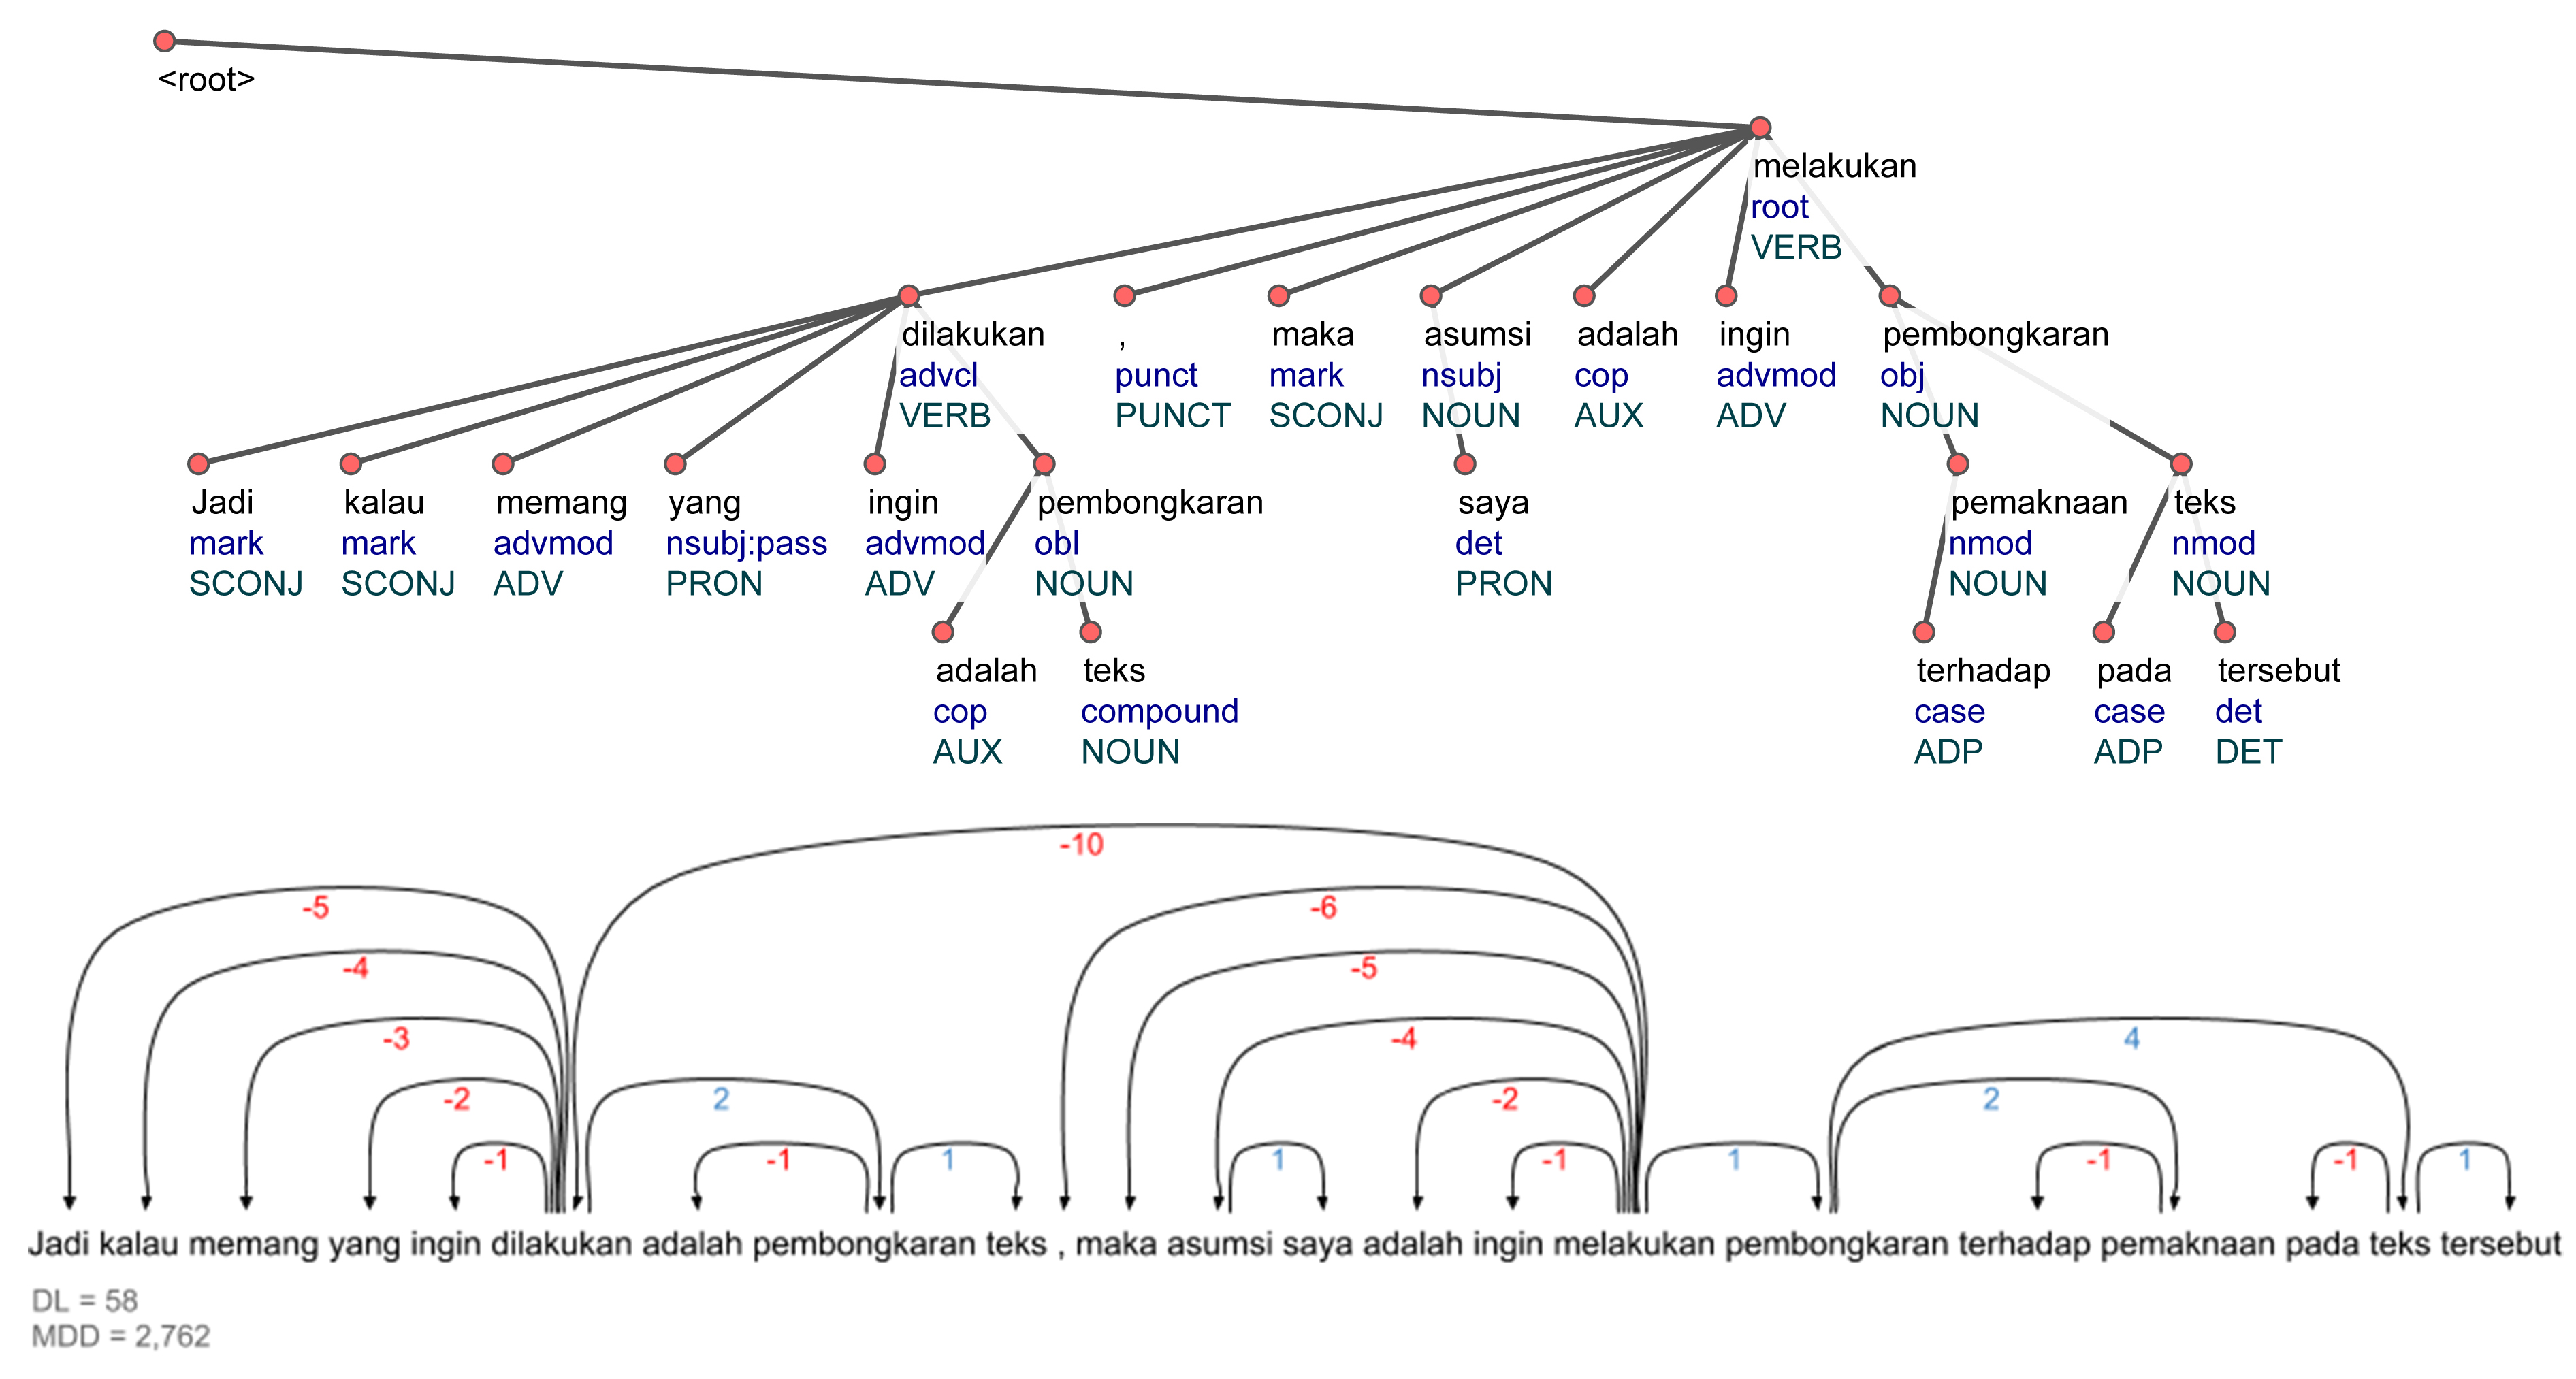
\includegraphics[width=1
	\textwidth] {pics/ls6521.jpg} 
	\caption{Kalimat L22 pada data ragam lisan} 
	\label{fig:ls6521} 
\end{figure}

Kalimat L22 (\pic~\ref{fig:ls6521}) memiliki akar verba \textit{melakukan} dan mengikat banyak konsituen terikat. Pada kalimat ini, terlihat bagaimana tautan dependensi dan percabangan jauh lebih menyebar dibandingkan dengan contoh-contoh kalimat dalam ragam tulis. Percabangan yang menyebar ini menyebabkan tautan-tautan dependensi berjarak jauh karena tautan dependensi antara dua konstituen yang berdampingan jumlahnya lebih sedikit dibandingkan dengan contoh-contoh pada ragam tulis. Dua percabangan utama terlihat pada simpai \textit{dilakukan} dan simpai pusat \textit{melakukan}. Penyebaran simpai-simpai ini juga berakibat pada tingkat kedalaman dependensi yang lebih dangkal dibandingkan dengan contoh-contoh pada ragam tulis. Akar \textit{melakukan} juga tidak memiliki aktor pelaku seperti pada contoh kalimat L4 (pic~\ref{fig:ls1102}). Pada kedua kasus ini, aktor pelaku terhadap verba-verba tersebut mungkin baru akan dimengerti dengan memahami relasi pada tataran diskursus. Kalimat L22 ini memiliki DL sejauh 57 dan MDD sejauh 2,714 konstituen. 

\begin{figure}
	\centering 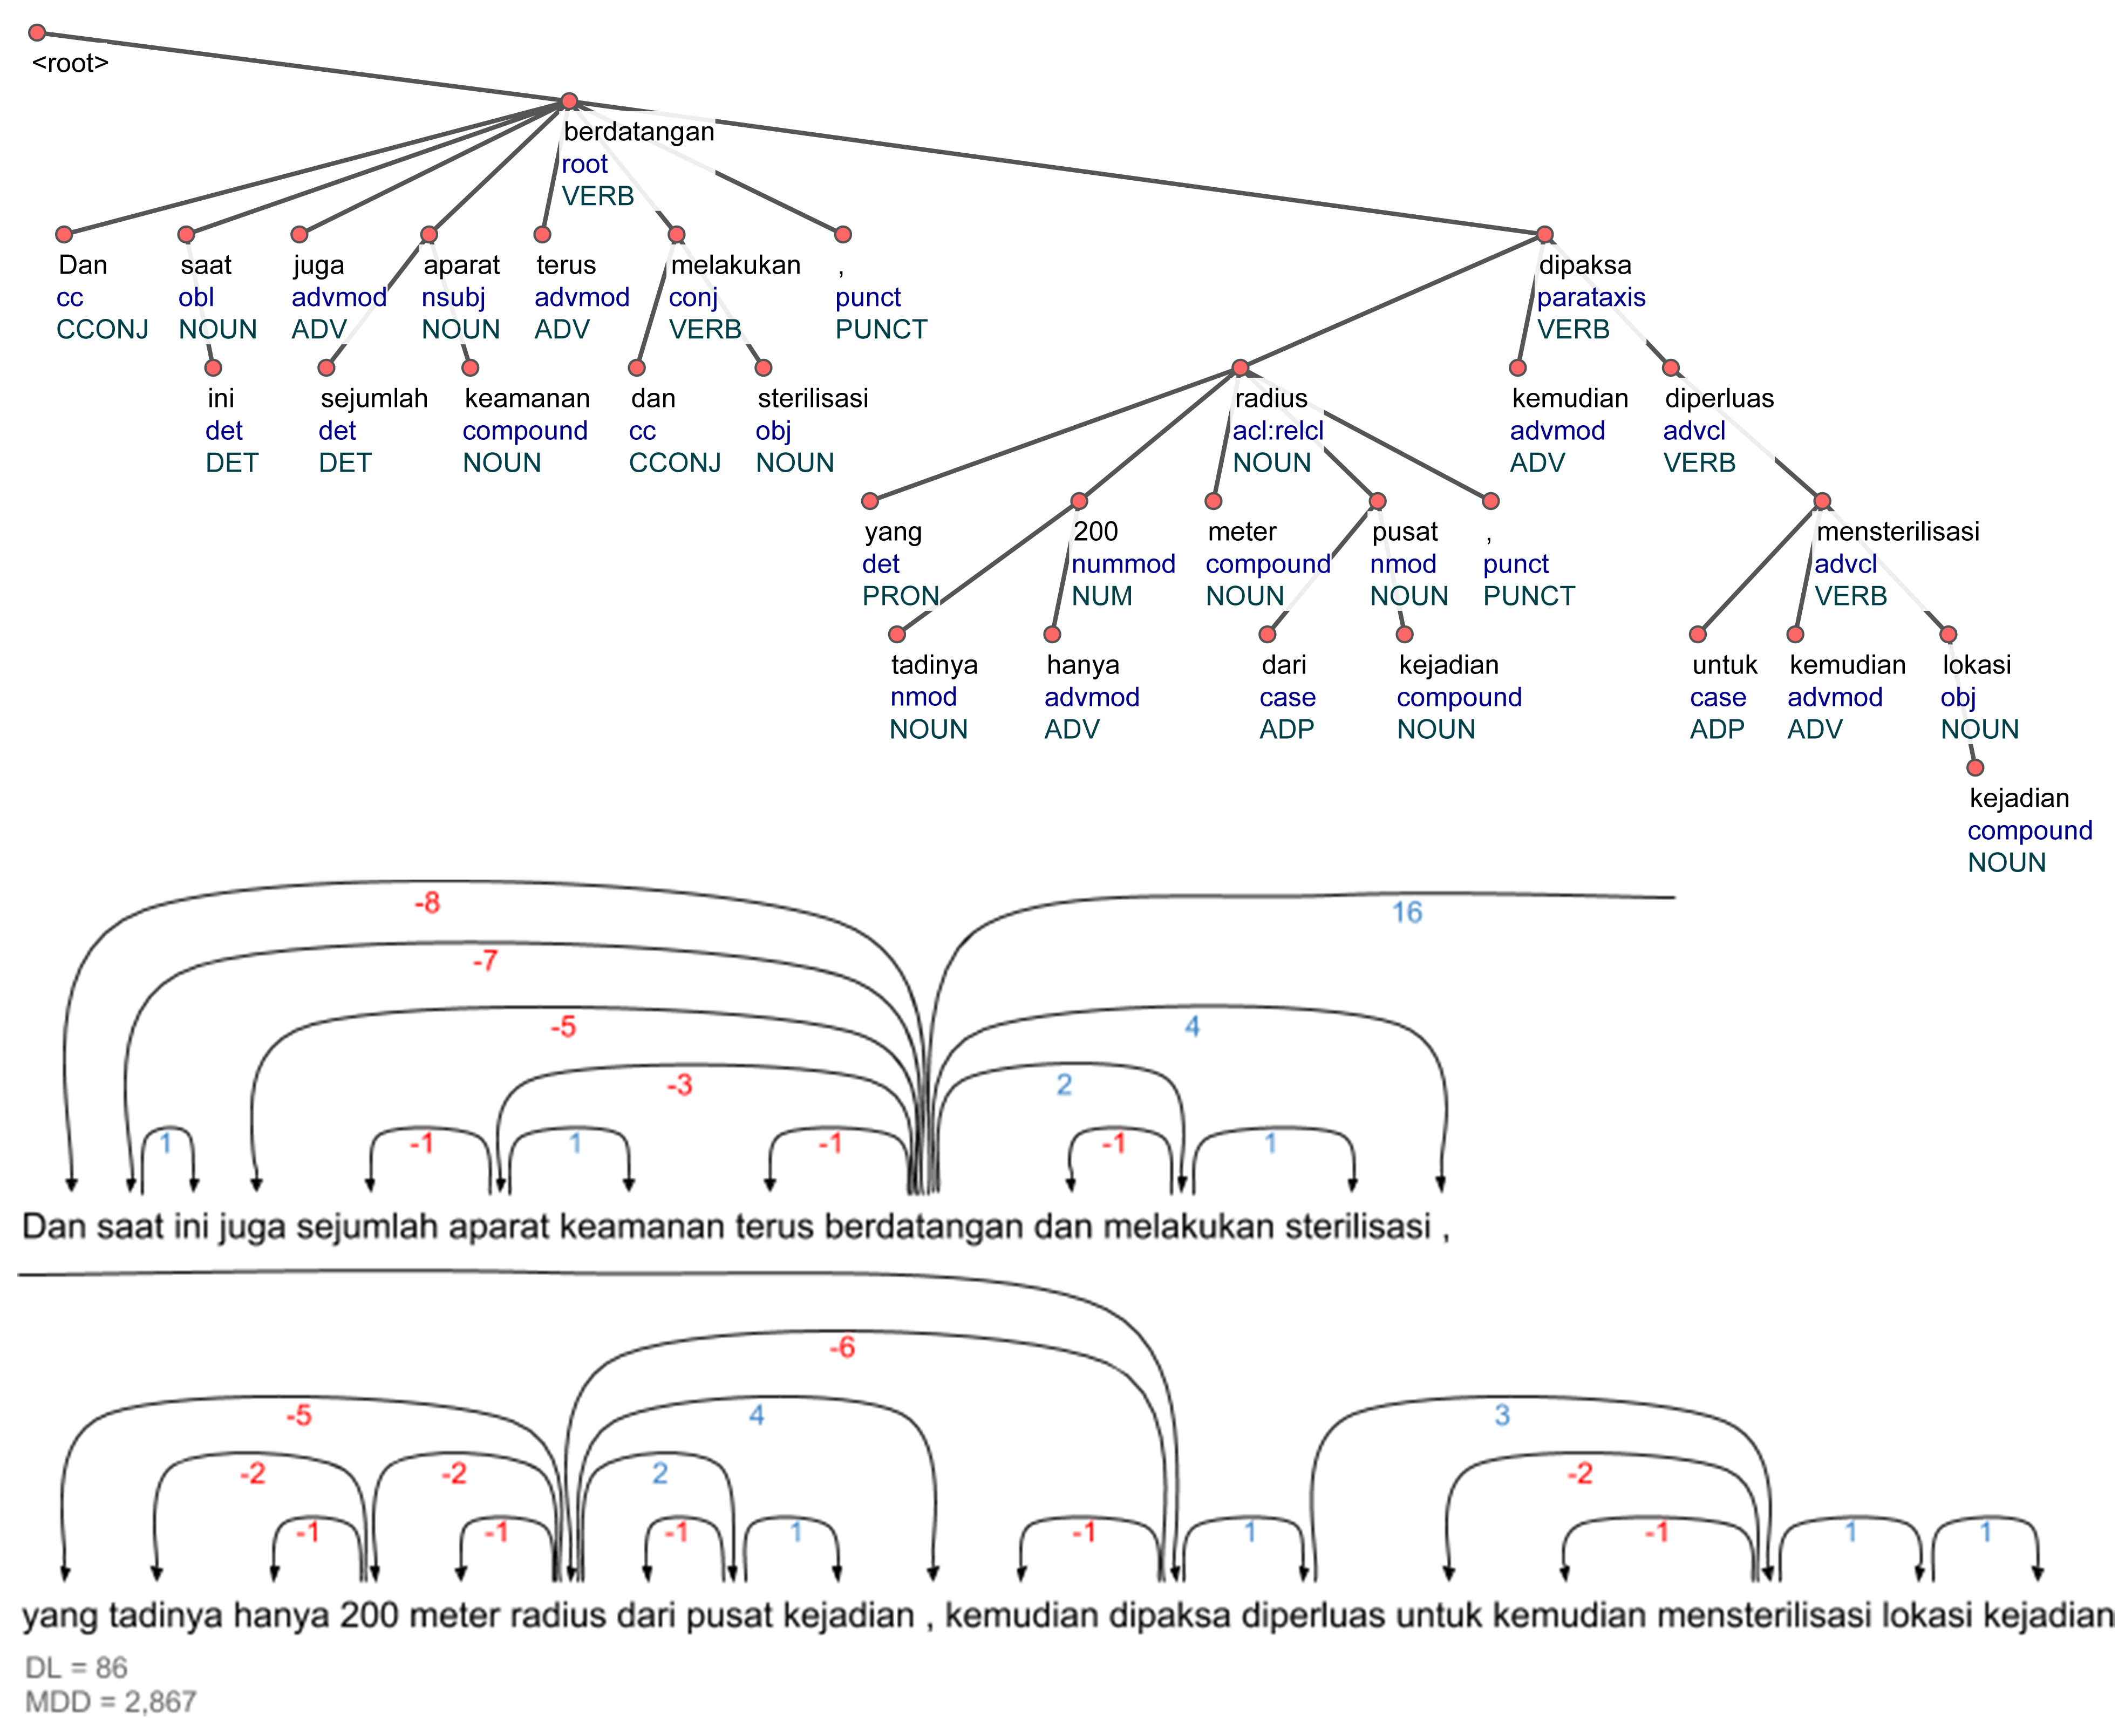
\includegraphics[width=1
	\textwidth] {pics/ls1716.jpg} 
	\caption{Kalimat L31a pada data ragam lisan} 
	\label{fig:ls1716} 
\end{figure}

Pada kalimat L31a (\pic~\ref{fig:ls1716}), simpai pusat dan simpai cabang pada verba \textit{dipaksa} memiliki banyak tautan yang juga cukup menyebar dibandingkan dengan contoh kalimat pada ragam tulis. Kalimat ini memperlihatkan adanya pembagian informasi secara besar seperti pada kalimat L22. Relasi akar verbal \textit{berdatangan} dengan verba \textit{dipaksa} memiliki tipe dependensi $parataxis$. Tipe ini menandakan relasi yang menyerupai koordinasi antar diskursus, dalam arti seluruh informasi yang dibawa oleh simpai konstituen terikat ini memiliki kualitas kalimat utuh sehingga bisa menjadi kalimat terpisah. Kalimat L31a (\pic~\ref{fig:ls1716}) memiliki DL sejauh 86 dan MDD sejauh 2,867 konstituen. 

\begin{figure}
	\centering 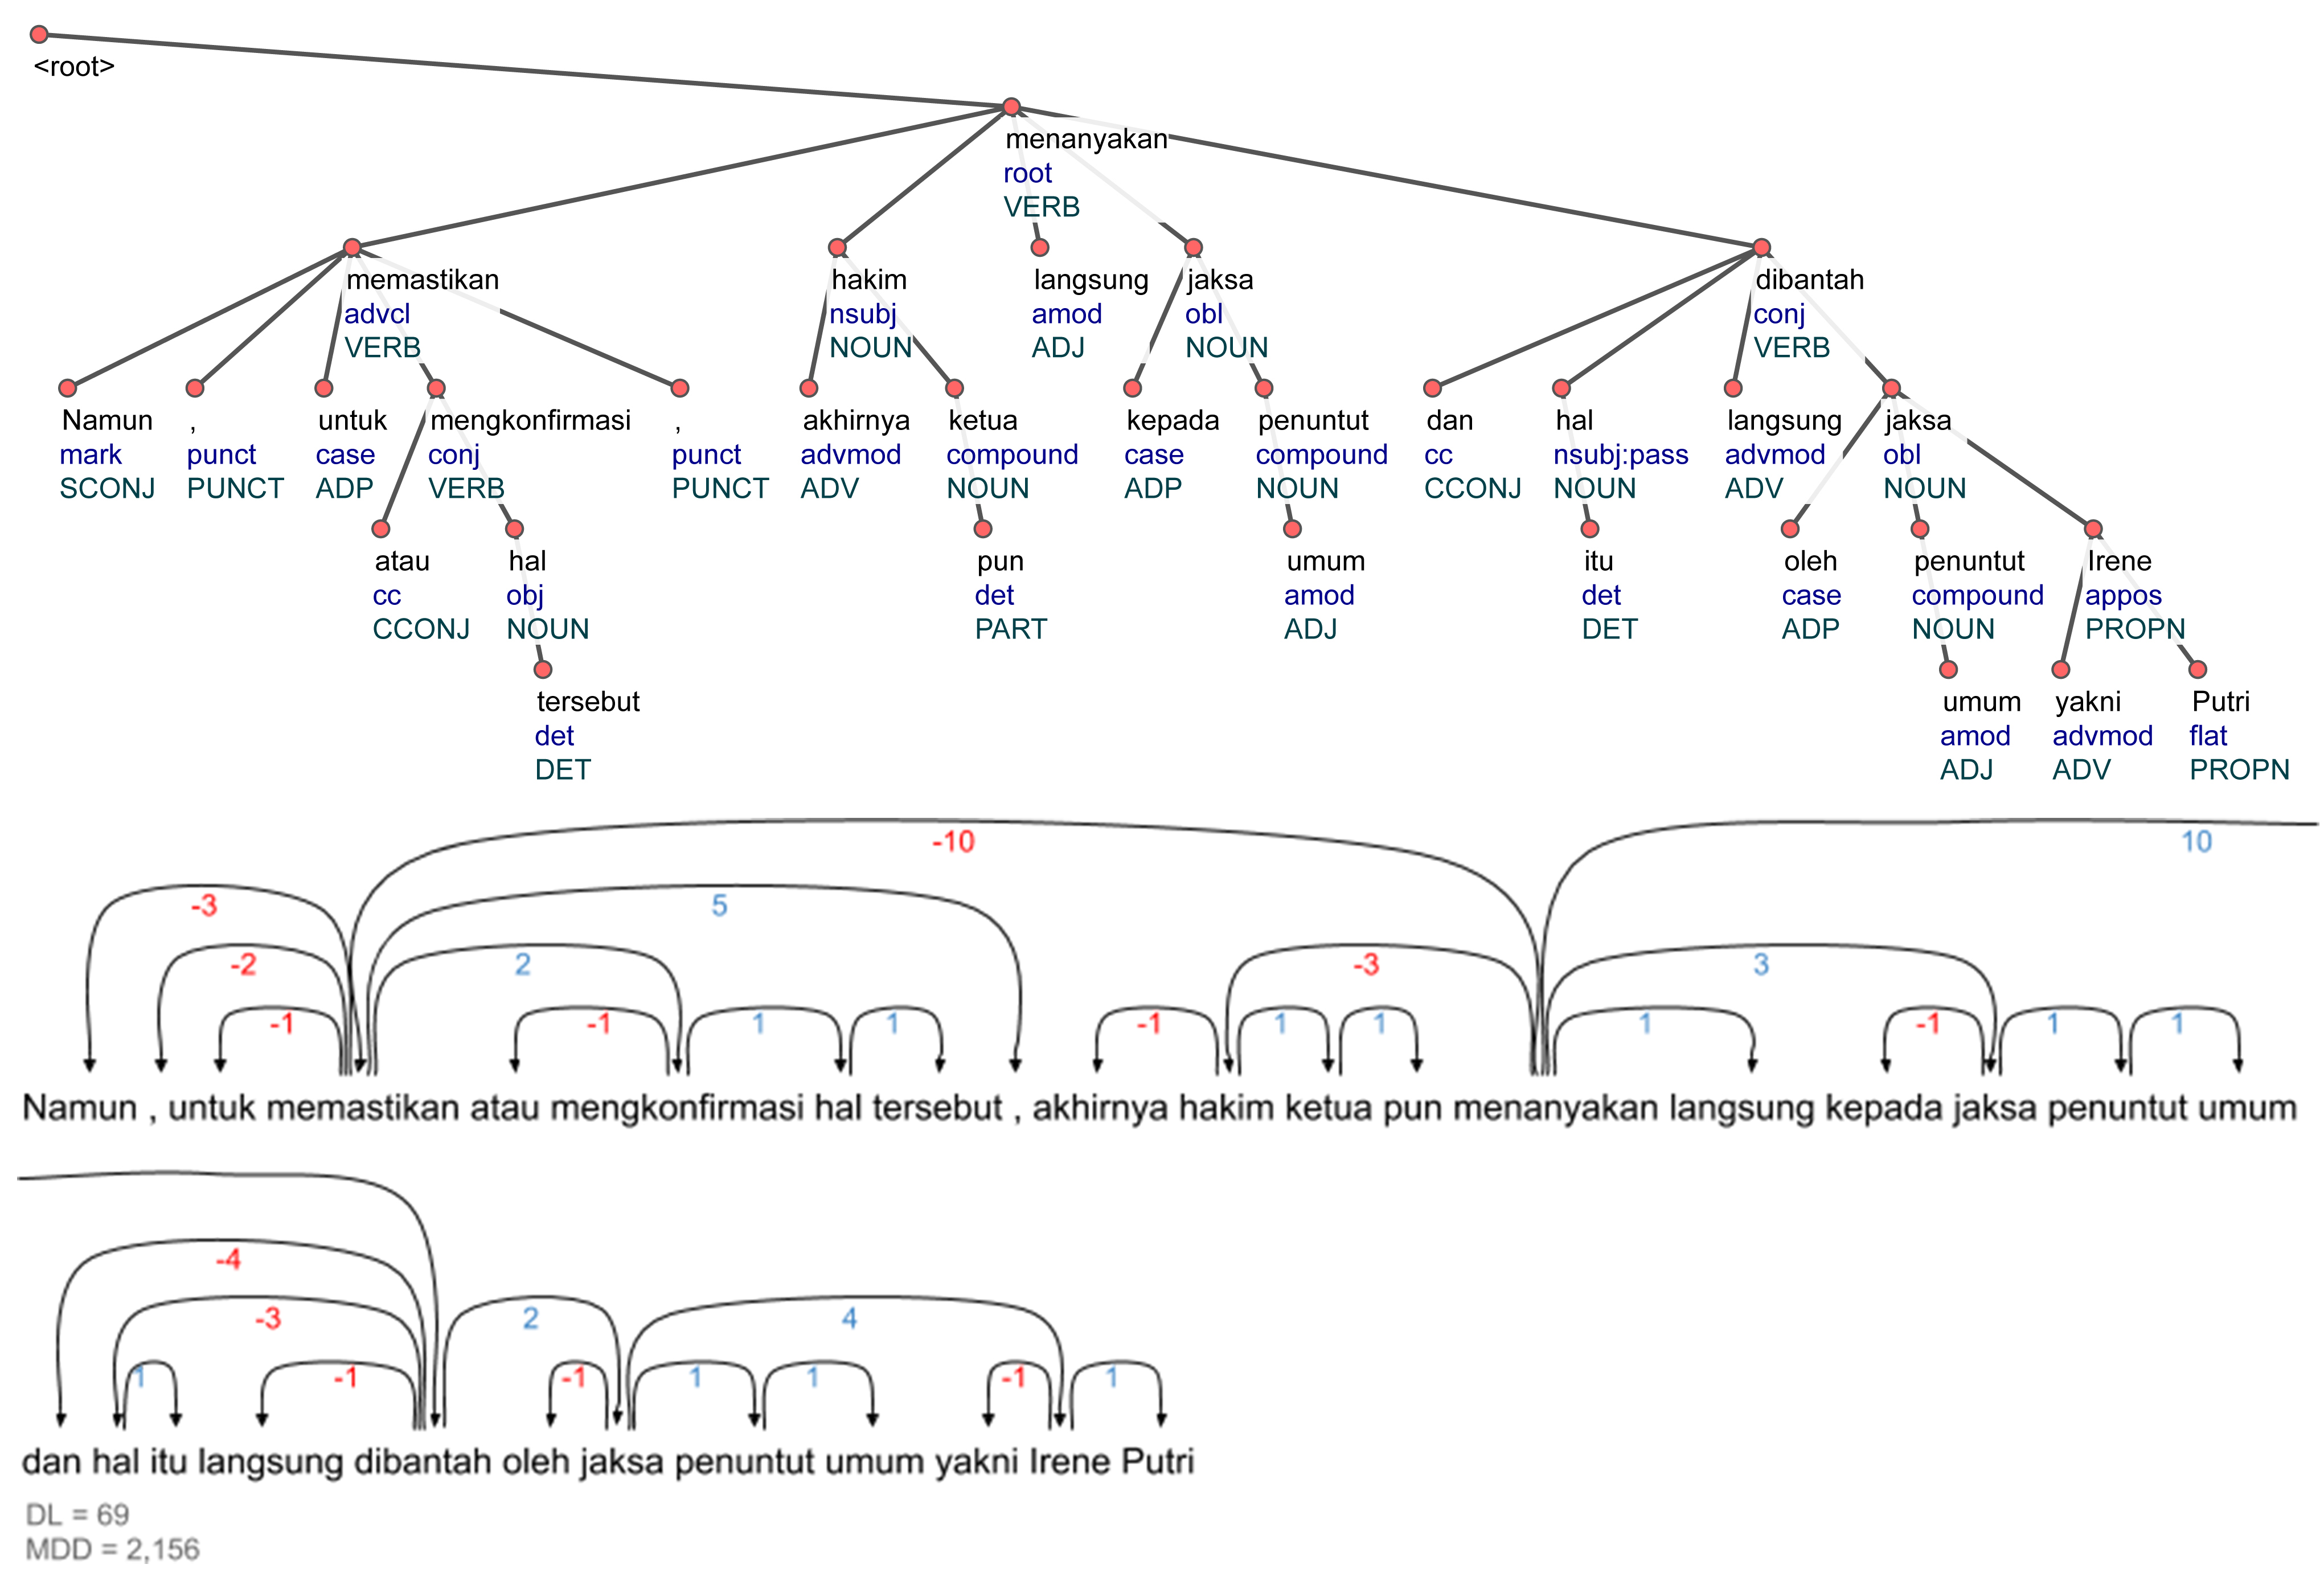
\includegraphics[width=1
	\textwidth] {pics/ls16.jpg} 
	\caption{Kalimat L31b pada data ragam lisan}
	\label{fig:ls16} 
\end{figure}

Pada kalimat L31b (\pic~\ref{fig:ls16}), posisi akar berada di tengah kalimat. Seluruh informasi yang dibawa klausa tujuan dengan induk \textit{memastikan} direalisasikan sebelum akar verbal \textit{menanyakan}. Akar verbal ini juga mengikat verba \textit{dibantah} yang dihubungkan dengan konjungsi \textit{dan}. Kalimat ini tidak memiliki kandungan informasi yang bersifat diskursus seperti kalimat L31b, namun jumlah simpai-simpai cabang di bawah \textit{memastikan}, \textit{menanyakan}, dan \textit{dibantah} juga tersebar cukup merata. Kalimat L31b (\pic~\ref{fig:ls16}) memiliki DL sejauh 67 dan MDD sejauh 2,233 konstituen. Seperti kalimat T31b, selisih DL dari tautan-tautan dependensi positif dan negatif sangat kecil (sebesar 3) sehingga juga menandakan jumlah bentuk relasi diawali induk dan jumlah bentuk relasi diakhiri induk yang cukup seimbang. 

\begin{figure}
	\centering 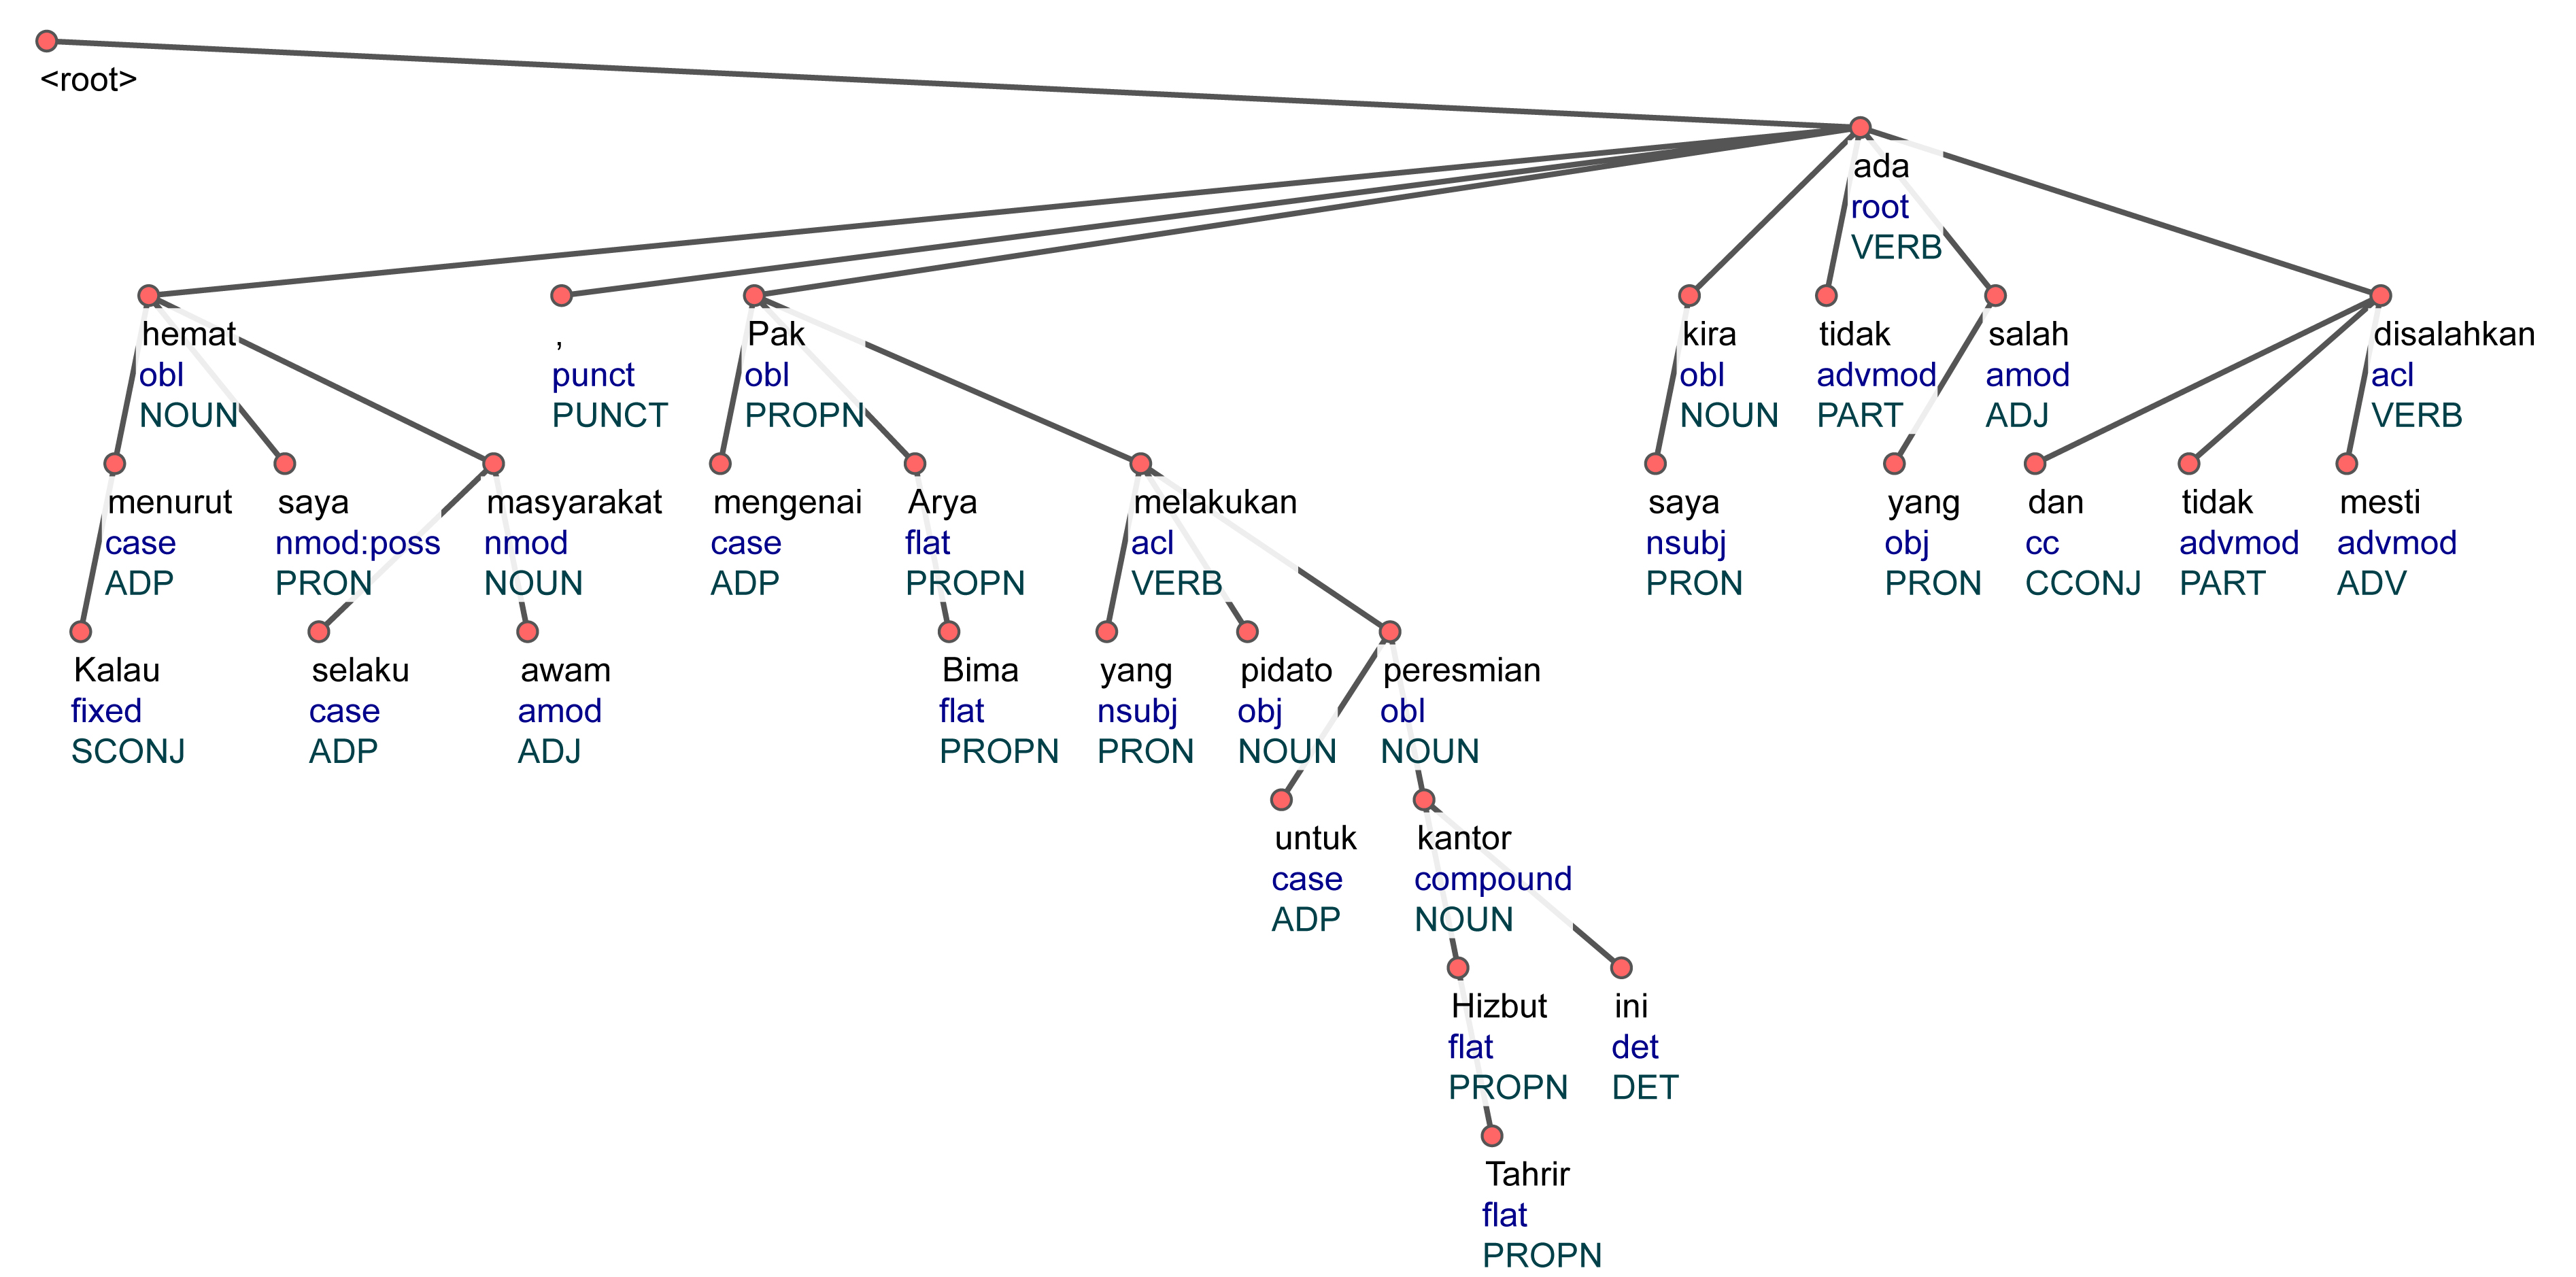
\includegraphics[width=1
	\textwidth] {pics/ls114.jpg} 
	\caption{Kalimat L31c pada data ragam lisan}
	\label{fig:ls114} 
\end{figure}

Posisi akar pada kalimat L31c (\pic~\ref{fig:ls114}) cenderung berada di akhir seperti pada kalimat L22. Hal ini berarti semua simpai-simpai cabang di bawah \textit{hemat} dan \textit{Pak} harus disimpan di dalam memori kerja sebelum akar verbal \textit{kira} direalisasikan. Di bawah simpai \textit{Pak}, terlihat adanya indikasi percabangan searah, yaitu relasi antara \textit{Pak} dengan \textit{melakukan} dan \textit{melakukan} dengan \textit{peresmian}, dan seterusnya. Namun seluruh relasi ini berada di bawah tautan utama antara \textit{ada} dengan \textit{Pak}, sehingga terjadi percabangan yang bersifat kombinasi antara searah dan beda arah. Kalimat L31c (\pic~\ref{fig:ls114}) memiliki DL sejauh 100 dan MDD sejauh 3,333 konstituen. Selisih nilai DL dari tautan-tautan dependensi positif dan negatif sangat besar yaitu -40. Nilai negatif ini menandakan jumlah bentuk relasi diakhiri induk yang jauh lebih besar dibandingkan sebaliknya. Tampak pada \pic~\ref{fig:ls114}, nilai negatif yang besar ini terutama disebabkan oleh tautan-tautan dependensi pada simpai pusat yang sangat jauh.

Kalimat L22 (\pic~\ref{fig:ls6521}), L31a (\pic~\ref{fig:ls1716}), L31b (\pic~\ref{fig:ls16}), dan L31c (\pic~\ref{fig:ls114}) sedikit berbeda satu sama lain, namun memiliki karakter utama yang serupa yang membedakannya dengan contoh-contoh kalimat pada data ragam tulis. Salah satunya adalah perbedaan posisi akar pada \pic~\ref{fig:ls6521}, \pic~\ref{fig:ls1716}, \pic~\ref{fig:ls16}, dan \pic~\ref{fig:ls114}. Berdasarkan beberapa visualisasi bank pohon struktur tersebut, perbedaan yang paling terlihat antara contoh-contoh pada ragam lisan dibandingkan dengan contoh-contoh pada ragam tulis adalah percabangannya yang terlihat lebih tidak konsisten. Meskipun tidak semua kalimat memiliki struktur seperti \pic~\ref{fig:ts2079} dan \pic~\ref{fig:ts2081}, mayoritas kalimat panjang pada data ragam tulis menunjukkan karakter yang lebih konsisten dalam hal pergerakan percabangannya. Pada data ragam lisan, terlihat banyak kombinasi antara percabangan searah dan beda arah serta letak posisi akar yang menyebar dari awal hingga akhir kalimat. Percabangan utama yang tersebar pada ketiga kalimat tersebut menunjukkan indikasi hubungan klausa yang tidak bersifat berlanjut, namun paralel. Kalimat L22 (\pic~\ref{fig:ls6521}), L31b (\pic~\ref{fig:ls16}) dan L31c (\pic~\ref{fig:ls114}) memiliki percabangan utama sebelum akar sehingga secara kolektif membentuk relasi dependensi utama yang negatif. Hal ini berarti seluruh informasi yang dibawa oleh klausa-klausa pada simpai dan percabangan sebelum akar harus disimpan dalam memori kerja dan menunggu realisasi akar yang mengandung informasi utama untuk dapat bermakna secara utuh \citep{hawkins2014cross}.

%%-----------------------------------------------------------------------------%
\subsection{Pengaruh panjang kalimat terhadap panjang dependensi kalimat dan rata-rata jarak dependensi antarkonstituen}
%%-----------------------------------------------------------------------------%
Berdasarkan percobaan acak yang dilakukan, langkah analisis pada bagian ini adalah melihat aspek-aspek yang mungkin mempengaruhi struktur kalimat sehingga memungkinkan terjadinya DLM dan DDM. Secara garis besar, analisis lanjutan untuk melihat aspek-aspek ini menghasilkan temuan strategi yang berkaitan dengan panjang kalimat, pengaturan urutan kata terkait pendekatan dan penempatan posisi, serta pengurangan valensi. Ketiga aspek besar ini menjawab pertanyaan-pertanyaan penelitian yang diajukan pada Bab 1. Langkah analisis pada bagian ini mencoba meninjau pengaruh panjang kalimat atau jumlah konstituen terhadap panjang dependensi kalimat dan jarak dependensi antarkonstituen serta struktur kalimat yang terbentuk dalam kedua korpus. Temuan utama yang muncul adalah dalam kondisi tertentu, perbandingan DL dan MDD antara kedua korpus data memiliki karakteristik yang berbeda. Rata-rata jumlah konstituen pada data ragam tulis berada antara 17 hingga 18 (\textit{mean} = 17,423) dan antara 10 hingga 11 konstituen (\textit{mean} = 10,859) pada ragam lisan dengan perbedaan yang signifikan (\textit{P} \textless 0,001). Perbedaan ini menunjukkan bahwa ada kecenderungan penutur memilih jumlah konstituen yang lebih sedikit saat merealisasikan kalimat secara lisan. Klasifikasi kalimat pendek, menengah, dan panjang dilakukan berdasarkan penelitian terdahulu dari \cite{gildea2015human}, \cite{futrell2015large}, \cite{wang2017effects}, serta \cite{liu2017dependency}. Berdasarkan data masing-masing penelitian tersebut, temuan-temuan yang didapat menyebutkan bahwa ada perbedaan perilaku dan karakteristik sintaksis yang dipengaruhi panjang kalimat. Berdasarkan klasifikasi panjang kalimat pada penelitian ini yang dilakukan bertitik tolak dari temuan-temuan tersebut, temuan analisis ini juga menemukan hasil yang serupa. 

Pada klasifikasi kalimat pendek (maksimal 10 konstituen dalam sebuah kalimat), perbedaan rata-rata panjang dan jarak dependensi antara ragam tulis dan lisan tampak dipengaruhi oleh pemusatan data ragam lisan. Kalimat-kalimat dalam kedua korpus sama-sama mengalami optimasi urutan kata yang menyebabkan terjadinya DLM dan DDM.  Namun, kecenderungan untuk menggunakan kalimat pendek menyebabkan data ragam lisan memiliki rata-rata DL dan MDD yang lebih pendek secara signifikan terutama hingga panjang kalimat sebanyak 5 konstituen. Pada pengamatan yang lebih dalam, ditemukan bahwa mulai jumlah konstituen sebanyak 6, data ragam tulis justru menunjukkan MDD yang lebih pendek secara signifikan. Tinjauan secara kualitatif mengindikasikan adanya perbedaan tingkat kedalaman dependensi antara kedua ragam pada contoh-contoh kalimat dengan jumlah konstituen sebanyak 4. Meskipun begitu, tidak ditemukan karakteristik struktur yang unik yang dapat membedakan keduanya secara signifikan tidak ditemukan. Struktur sintaksis dan pengaturan klausa bebas serta terikat pada kedua ragam juga tidak berbeda secara signifikan. Keserupaan ini mungkin disebabkan oleh keterbatasan jumlah konstituen dan bentuk-bentuk kalimat yang hanya mengandung satu klausa bebas sehingga kompleksitas kalimat-kalimat tersebut masih rendah. Meskipun begitu, terlihat indikasi adanya pengurangan atau reduksi konstituen pada data ragam lisan berupa subyek atau aktor pelaku. Tinjauan lebih dalam mengenai pengurangan valensi ini akan dibahas pada tahap analisis berikutnya.

Terdapat temuan yang menarik pada klasifikasi kalimat menengah, yaitu rata-rata DL dan MDD antara kedua korpus data yang berbanding terbalik. Rata-rata DL yang dihasilkan korpus data ragam lisan lebih pendek dibandingkan ragam tulis namun tidak berbeda secara signifikan. Sebaliknya, rata-rata MDD yang didapatkan korpus data ragam tulis lebih pendek dibandingkan ragam lisan dan berbeda secara signifikan. Asumsi perbedaan kedua nilai ini merupakan alasan mengapa kedua pendekatan digunakan pada penelitian ini. Berdasarkan temuan ini, perbedaan kedua pendekatan dapat memberikan temuan awal untuk melihat kesesuaiannya dalam mengukur efisiensi memori kerja yang tercermin pada struktur sintaksis sebuah kalimat. Rata-rata DL dan MDD yang berbanding terbalik ini mengindikasikan bahwa meskipun jumlah total panjang dependensi lebih jauh dalam satu klasifikasi karena jumlah konstituen yang lebih banyak, struktur kalimat yang lebih efisien dapat menghasilkan rata-rata jarak dependensi antarkonstituen yang lebih pendek. Dalam hal ini, data ragam tulis sudah mulai memperlihatkan struktur kalimat yang lebih efisien dibandingkan ragam lisan. Rata-rata jumlah konstituen antara kedua korpus data berbeda secara signifikan yang berarti pada klasifikasi ini, penutur masih memiliki kecenderungan atau preferensi untuk mengurangi panjang kalimat saat merealisasikan kalimat secara lisan. Berdasarkan temuan ini, muncul asumsi bahwa DL berguna untuk menggambarkan kompleksitas sebuah kalimat secara umum dan MDD berguna untuk mewakili bagaimana efisiensi struktur kalimat melalui tautan dependensi antarkonstituennya.

Pada klasifikasi kalimat panjang, kedua rata-rata DL dan MDD pada korpus data ragam tulis lebih pendek dibandingkan ragam lisan dan berbeda secara signfikan. Hal ini berarti ada indikasi bahwa struktur kalimat-kalimat ragam tulis lebih efisien dilihat baik dari segi kompleksitas kalimat maupun jarak antarkonstituen yang dapat mewakili bentuk strukturnya. Perbedaan rata-rata jumlah konstituen antara kedua korpus tidak signifikan yang berarti pada klasifikasi ini, tidak ada kecenderungan atau preferensi penutur terhadap panjang kalimat terkait ragam tertentu. Tinjauan lebih dalam dilakukan untuk mengamati struktur-struktur kalimat yang umum ditemukan pada kedua korpus data. Berdasarkan analisis yang bersifat kualitatif terhadap struktur kalimat-kalimat \pic~\ref{fig:ts3901}, \pic~\ref{fig:ts2079}, \pic~\ref{fig:ts2081}, \pic~\ref{fig:ls6521}, \pic~\ref{fig:ls1716}, \pic~\ref{fig:ls16}, dan \pic~\ref{fig:ls114}, terlihat ada perbedaan yang cukup mendasar antara kedua ragam. 

Pada struktur kalimat panjang ragam tulis, banyak ditemukan kalimat yang hanya memiliki satu simpai cabang terdekat meskipun mengandung banyak klausa terikat sehingga kompleksitas kalimat tergolong tinggi. Hal ini juga terlihat pada berbedaan tingkat kedalaman dependensi antara kedua ragam. Pengaturan urutan kata pada bentuk struktur sintaksis seperti pada ragam tulis mencerminkan percabangan searah dan mengakibatkan hubungan-hubungan antarklausanya bersifat berlanjut. Contoh-contoh pada ragam tulis juga menunjukkan jumlah tautan dependensi antara dua konstituen yang berdampingan yang lebih banyak dibandingkan pada ragam lisan. Berkaitan dengan teori dependensi \citep{tesniere1959elements, hawkins2014cross, gildea2010grammars}, hubungan seri ini dilakukan untuk menambahkan informasi secara bertahap sehingga tautan dependensinya lebih pendek. 

Struktur sintaksis yang ditemukan pada kalimat-kalimat ragam tulis ini juga memilki posisi akar relatif paling awal. Oleh karena itu, seiring jalannya kalimat direalisasikan, informasi yang diproduksi setelahnya bersifat tambahan karena akar (konstituen yang mengandung informasi utama) sudah direalisasikan sejak awal. Berbeda dengan ragam tulis, struktur-struktur kalimat dalam data ragam lisan ditemukan tidak konsisten dan berbeda satu sama lain. Posisi akar dapat berada di depan, tengah, maupun akhir dan banyak ditemukan kalimat dengan banyak simpai cabang pada tingkat tautan dependensi utama. Relasi $parataxis$ dengan akar juga ditemukan yang berarti simpai cabang memiliki kualitas diskursus dan dapat menjadi kalimat lepas namun bergabung menjadi satu kalimat. Simpai-simpai cabang ini juga mengakibatkan klausa-klausa terikat tersebar secara paralel yang mungkin juga menyebabkan tingkat kedalaman dependensi pada ragam lisan ini lebih dangkal dibandingkan ragam tulis. Pada beberapa kalimat, ditemukan kombinasi percabangan yang bersifat searah maupun beda arah, tetapi kemunculannya juga tidak konsisten. Terutama pada akar yang berada di akhir kalimat, klausa-klausa yang terikat pada simpai-simpai cabang sebelumnya harus disimpan dulu di memori kerja hingga akar yang mengandung informasi utama direalisasikan dalam kalimat. 

Terdapat satu kalimat contoh dari korpus ragam tulis yang panjang dan jarak dependensinya sama dengan salah satu kalimat dari korpus ragam lisan. Namun, kedua kalimat ini memiliki struktur sintaktis yang jauh berbeda. Perbedaan utama kedua kalimat tersebut terletak pada tingkat kedalaman dependensi yang diakibatkan oleh perbedaan konstruksi kalimat. Perbedaan ini juga dapat terlihat pada visualisasi bank pohon struktur dependensi kedua kalimat. Kalimat ragam tulis menunjukkan percabangan yang bergerak searah semakin ke bawah sehingga menghasilkan tingkat kedalaman dependensi yang berlapis-lapis. Sementara itu, kalimat ragam lisan menunjukkan percabangan yang menyebar dengan pembagian cabang yang cukup merata sehingga menghasilkan tingkat kedalaman dependensi yang lebih dangkal. Temuan ini sangat menarik karena menimbulkan pertanyaan bahwa meskipun panjang dan jarak dependensi dua kalimat sama, apakah penutur tetap akan cenderung memilih satu bentuk konstruksi dibandingkan yang lain. Pertanyaan ini membutuhkan penelitian lanjutan yang melibatkan uji persepsi.

Secara umum, perbandingan analisis pada ketiga klasifikasi memberikan informasi yang berarti. Perbedaan yang ditemukan pada ketiganya menandakan bahwa panjang kalimat berpengaruh terhadap panjang dependensi kalimat dan rata-rata jarak dependensi antarkonstituen. Namun, perbedaan karakter struktur sintaksis pada korpus data ragam tulis dan lisan baru terlihat jelas pada kalimat dengan kompleksitas lebih tinggi jumlah konstituen yang lebih banyak. \cite{wang2017effects} menemukan dalam penelitiannya bahwa data ragam tulis yang ditujukan untuk percakapan lisan (sebagai contoh dialog film) memiliki MDD yang lebih pendek dibandingkan teks yang lebih formal. \cite{wang2017effects} menindaklanjuti kajian yang dilakukan \cite{hiranuma1999syntactic} dan \cite{liu2009chinese} mengajukan asumsi bahwa pada teks yang semakin formal (berdasarkan data yang digunakan) lebih sulit secara sintaktis. Dalam penelitian ini, temuan serupa terjadi pada klasifikasi kalimat pendek (\textless= 5 konstituen) di mana ragam lisan memiliki DL dan MDD yang lebih pendek. Temuan serupa didapatkan oleh \cite{wang2017effects}, yang mengindikasikan bahwa kalimat-kalimat ragam lisan pada klasifikasi ini lebih mudah dimengerti secara sintaktis. Namun, asumsi ini tidak berlaku pada kalimat yang lebih panjang. 

Berdasarkan data yang dikumpulkan pada penelitian ini, pada klasifikasi menengah dan panjang, teks yang lebih formal (ragam tulis) justru menunjukkan efisiensi kalimat yang lebih tinggi mulai dari jumlah konstituen sebanyak 6 hingga 40. Merujuk pada \pic~\ref{fig:lisantulis_DL} dan \pic~\ref{fig:lisantulis_MDD}, kedua grafik menunjukkan gerak garis regresi yang berkebalikan antara ragam lisan dan tulis pada titik sekitar panjang kalimat sebanyak 40 konstituen. Namun, signifikansi yang melemah dan cenderung berbalik pada panjang kalimat di atas 40 konstituen mungkin disebabkan oleh persebaran data kedua korpus yang sangat sedikit pada rentang tersebut, terutama pada data ragam lisan. Penelitian lanjutan untuk rentang panjang kalimat tersebut membutuhkan data dengan jumlah yang cukup besar dan seimbang pada kedua korpus, namun kalimat yang sangat panjang cukup jarang ditemukan dalam ragam lisan. Hal ini dapat dikaitkan dengan kecenderungan pada ragam lisan untuk menggunakan kalimat-kalimat yang pendek. Analisis kualitatif terhadap perbedaan karakteristik sintaksis pada klasifikasi kalimat panjang memperlihatkan secara jelas bagaimana perbedaan struktur kalimat pada kedua ragam, terutama terkait tingkat kedalaman dependensi, tautan dependensi dari dua konstituen yang berdampingan, dan reduksi sintaktik atau reduksi konstituen pada ragam lisan yang menyebabkan panjang kalimat menjadi lebih pendek.

%%-----------------------------------------------------------------------------%
\section{Direksionalitas induk dan valensi akar verbal}
%%-----------------------------------------------------------------------------%
Pada pembahasan temuan-temuan di atas, sudah dibahas sedikit mengenai struktur kalimat terkait posisi akar dan pola percabangannya. Seperti yang dijelaskan sebelumnya, belum ada konvensi mengenai direksionalitas induk terkait hierarki dan pengolahan dalam memori kerja. Jarak dependensi positif dihasilkan dari bentuk relasi induk sebelum konstituen terikat, dan sebaliknya, nilai dependensi negatif dihasilkan dari bentuk relasi induk setelah konstituen terikat. Bahasa Indonesia memiliki urutan kata yang cenderung bebas \citep{sneddon2010indonesian} dan dalam aturan tata bahasa yang mengadopsi prinsip struktur frasa, banyak urutan kata dalam aturan frasa yang memiliki kepala (\textit{head}) mendahului pewatas (\textit{modifier}) \citep{sneddon2010indonesian}. Akan tetapi, teori struktur frasa berbeda dengan dependensi dan belum ada penelitian yang melihat relasi induk dan konstituen terikat terkait arah dan posisi induknya (direksionalitas induk). 

Hipotesis yang digunakan pada beberapa penelitian yang melihat Pengurangan Panjang Dependensi (DLM) \citep{futrell2015large} serta Pengurangan Jarak Dependensi (DDM) \citep{liu2017dependency} menyebutkan bahwa kebebasan urutan kata ini mungkin dimanfaatkan oleh penutur menjadi strategi utama dalam menghasilkan kalimat yang efisien terutama mengenai penempatan konstituen pada posisi tertentu dalam urutan konstituen sebuah kalimat. Pada pembahasan ini, penghitungan DL tautan dependensi positif dipisahkan dengan tautan dependensi negatif. Bagian pertama analisis DL positif dan negatif melibatkan relasi dari semua konstituen dalam kalimat. DL positif dan negatif ini memberikan gambaran kasus tautan akar atau induk dengan konstituen terikat secara umum dan berkontribusi untuk membentuk asumsi kecenderungan karakteristik bahasa dilihat dari direksionalitas induknya \citep{wang2017effects}. 

\begin{figure}
\centering

\begin{subfigure}{.8\linewidth}
  \centering
  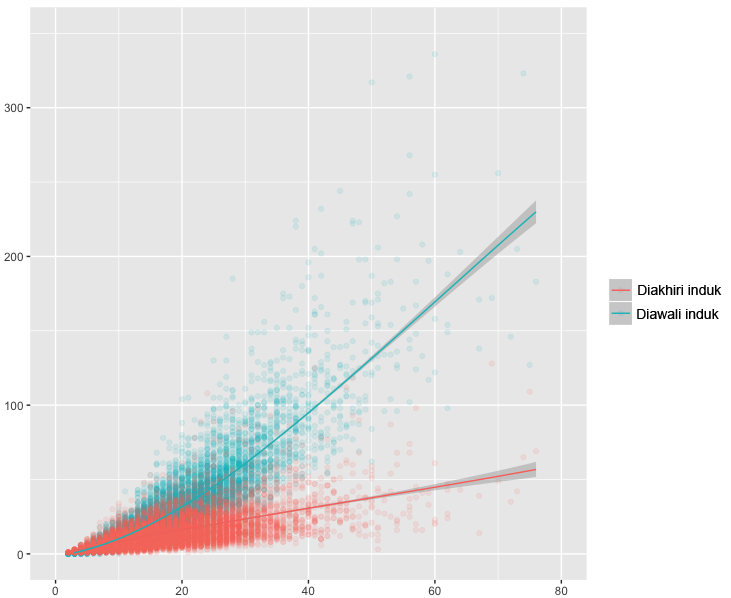
\includegraphics[width=1\linewidth] {pics/tulis_DLposneg.png} 
	\caption{Data ragam tulis}
	\label{fig:tulis_DLposneg} 
\end{subfigure}
%
\begin{subfigure}{.8\linewidth}
  \centering
  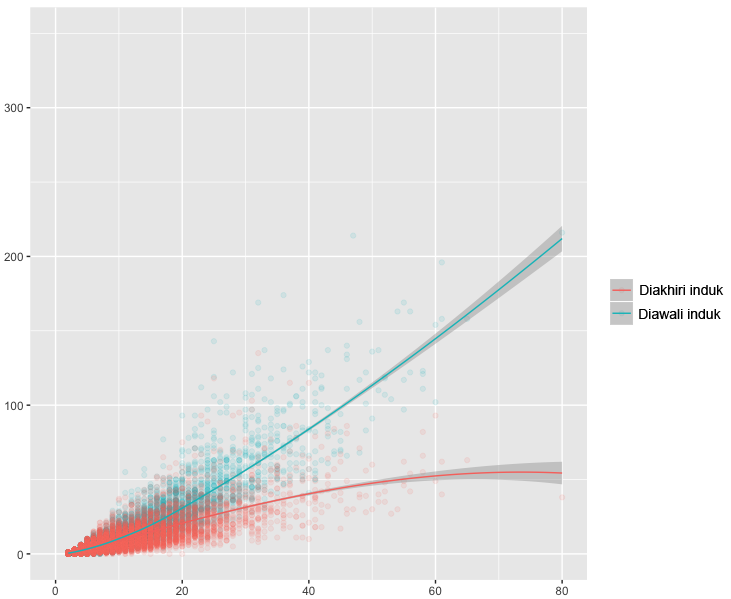
\includegraphics[width=1\linewidth]{pics/lisan_DLposneg.png} 
	\caption{Data ragam lisan}
	\label{fig:lisan_DLposneg} 
\end{subfigure}

\caption{Grafik panjang dependensi positif dan negatif data ragam tulis dan lisan}
\label{fig:DL_posneg}
\end{figure}

Berdasarkan \pic~\ref{fig:tulis_DLposneg} dan \pic~\ref{fig:lisan_DLposneg}, kedua korpus data menunjukkan garis regresi tautan dependensi positif yang berada jauh di atas garis regresi tautan dependensi negatif dan pada kalimat dengan jumlah konstituen yang semakin banyak, jarak antara keduanya semakin besar. Seperti yang dijelaskan sebelumnya, DL cukup sensitif terhadap panjang kalimat dan keduanya memiliki hubungan linear. Dalam sebuah kalimat, perbandingan jumlah bentuk relasi diawali dan diakhiri induk saling berkaitan. Hal ini berarti ada kecenderungan preferensi terhadap bentuk relasi diawali induk dan menandakan kesesuaian data observasi dengan tata bahasa yang berlaku. Namun, pada grafik DL ragam lisan (\pic~\ref{fig:lisan_DLposneg}), jarak garis regresi tautan dependensi positif dan negatif terlihat lebih dekat dibandingkan ragam tulis. Grafik ini juga memperlihatkan adanya kurva parabola terbuka ke bawah sehingga muncul asumsi adanya nilai tertinggi atau ambang batas (\textit{threshold}) terhadap panjang tautan dependensi negatif pada korpus data ragam lisan. Berdasarkan korpus data yang terkumpul, dugaan ambang batas tautan dependensi negatif ini menimbulkan asumsi bahwa mulai panjang kalimat tertentu, total tautan dependensi negatif dalam sebuah kalimat mungkin tidak akan melebihi nilai tertentu juga. 

\begin{table}
\begin{center}
\begin{small}
\caption{Frekuensi panjang dependensi positif dan negatif}  \label{tab:DLposneg}
\begin{tabular}{ | p{2cm} | p{2cm} | p{2cm} | p{2cm} | p{2cm} |}
\hline
Jumlah konstituen & Ragam tulis (+ \textgreater -) & Ragam tulis (+ \textless -) & Ragam lisan (+ \textgreater -) & Ragam lisan (+ \textless -) \\ \hline
\textless= 5 & 164 & 221 & 1188 & 1354 \\ \hline
6 - 10 & 992 & 646 &1469 & 1349 \\ \hline
11 - 20 & 3145 & 952 & 1858 & 1014 \\ \hline
21 - 30 & 1854 & 200 & 644 & 166 \\ \hline
31 - 40 & 558 & 36 & 204 & 37 \\ \hline
\textgreater 40 & 201 & 5 & 89 & 7 \\ \hline
 \end{tabular}
 \end{small}
 \end{center}
 \end{table}
 
\tab~\ref{tab:DLposneg} berisi frekuensi kalimat dengan melihat apakah kalimat tersebut memiliki DL positif yang lebih jauh atau sebaliknya. Hal ini berarti kalimat yang memiliki DL positif dan negatif sama jauh tidak diikutsertakan dalam analisis. Jumlah kalimat dalam \tab~\ref{tab:DLposneg} dihitung berdasarkan selisih panjang dependensinya. Berdasarkan tabel ini, kalimat yang DL positifnya lebih besar dari negatif ditemukan lebih banyak mulai dari panjang kalimat 6 konstituen. Hal ini memperlihatkan adanya kecenderungan terhadap bentuk relasi diawali induk. Selain itu, rasio perbandingan pada ragam tulis jauh lebih besar dibandingkan ragam lisan. Pada kategori kalimat terpanjang, jumlah kalimat yang DL positifnya lebih besar dapat mencapai 40 kali lebih banyak.  Temuan ini menunjukkan bahwa bentuk relasi diawali induk memiliki total jarak-jarak dependensi yang lebih besar dibandingkan bentuk relasi sebaliknya. Seiring bertambahnya jumlah konstituen, rasio frekuensi tautan dependensi positif dan negatif semakin besar pada kedua ragam. Namun, perbedaan rasio dari setiap kategori jumlah konstituen pada ragam lisan tidak sejauh ragam tulis. 

\begin{table}
\begin{center}
\begin{small}
\caption{Frekuensi tautan dependensi positif dan negatif}  \label{tab:tautanposneg}
\begin{tabular}{ | p{2cm} | p{2cm} | p{2cm} | p{2cm} | p{2cm} |}
    \hline
Jumlah konstituen & Ragam tulis (+) & Ragam tulis (-) & Ragam lisan (+) & Ragam lisan (-) \\ \hline
\textless= 5 & 677 & 700 & 2841 & 2764 \\ \hline
6 - 10 & 7023 & 5715 & 7649 & 6918 \\ \hline
11 - 20 & 35597 & 24426 & 15554 & 12898 \\ \hline
21 - 30 & 31036 & 18163 & 7564 & 5939 \\ \hline
31 - 40 & 12904 & 6968 & 3232 & 2414 \\ \hline
\textgreater 40 & 6583 & 3240 & 1928 & 1426 \\ \hline
   \end{tabular}
   \end{small}
\end{center}
\end{table}

\tab~\ref{tab:tautanposneg} merupakan tabel yang berisi frekuensi tautan dependensi positif dan negatif dalam kedua korpus data. Frekuensi ini hanya menggambarkan jumlah kemunculan tautan dan tidak memiliki jarak dependensi. Pada tabel ini, tautan-tautan dependensi tidak dikelompokkan per kalimat sehingga dapat memberikan gambaran jumlah tautan yang ada dalam keseluruhan korpus. Data ragam tulis menunjukkan bahwa mulai dari panjang kalimat 6 konstituen, frekuensi tautan dependensi negatif lebih sedikit dibandingkan tautan dependensi positif. Meskipun begitu, tautan dependensi positif lebih banyak pada semua klasifikasi dalam ragam lisan. Pada kategori kalimat terpanjang dalam ragam tulis, frekuensi tautan dependensi positif dapat mencapai dua kali tautan dependensi negatif. Sementara pada ragam lisan, perbandingan terbesar hanya mencapai 1,35 banding 1 sehingga juga menunjukkan indikasi bahwa kecenderungan bentuk relasi diawali induk lebih terlihat pada data ragam tulis. Rasio dengan jumlah tautan dependensi pada tabel ini memperlihatkan perbandingan yang tidak seekstrim rasio dengan jumlah kalimat pada tabel sebelumnya. Hal ini menandakan bahwa pada kalimat yang semakin panjang, bentuk relasi diawali induk lebih banyak digunakan oleh penutur bahasa Indonesia dan dalam satu kalimat, panjang dependensi dari tautan dependensi positif dapat memiliki nilai yang jauh lebih besar.

\begin{table}
\begin{center}
\begin{footnotesize}
\caption{Jarak dependensi seluruh tautan antarkonstituen}  \label{tab:deskriptif-konstituen}
\begin{tabular}{| c | llll | llll | l |}
\hline
 & \multicolumn{4}{c |}{+} & \multicolumn{4}{c |}{-} & \\  \cline{2-9}  
Panjang kalimat & min & med	& max & mean & min & med & max & mean & \\ \cline{1-10}  
\textless= 5 	& 1 & 1 & 4 & 1,409 	& 1 & 1 & 4 & 1,606 & \multirow{6}{*}{Tulis}\\
6 - 10 		& 1 & 1 & 9 & 1,866 	& 1 & 1 & 9 & 1,948 & \\
11 - 20 		& 1 & 1 & 19 & 2,468 & 1 & 1 & 19 & 2,147 & \\
21 - 30 		& 1 & 1 & 29 & 2,971 & 1 & 1 & 29 & 2,241 & \\ 
31 - 40 		& 1 & 1 & 39 & 3,597 & 1 & 1 & 37 & 2,299 & \\
\textgreater 40 & 1 & 1 & 68 & 4,22 	& 1 & 1 & 55 & 2,282 & \\ 
\hline
\textless= 5 	& 1 & 1 & 4 & 1,466 	& 1 & 1 & 4 & 1,534 & \multirow{6}{*}{Lisan}\\
6 - 10 		& 1 & 1 & 9 & 1,933 	& 1 & 1 & 9 & 2,071 & \\
11 - 20 		& 1 & 2 & 19 & 2,535 & 1 & 1 & 19 & 2,321 & \\
21 - 30 		& 1 & 2 & 28 & 3,263 & 1 & 1 & 27 & 2,5 & \\ 
31 - 40 		& 1 & 2 & 37 & 3,718 & 1 & 1 & 32 & 2,657 & \\
\textgreater 40 & 1 & 2 & 66 & 4,067 	& 1 & 1 & 46 & 2,438 & \\ 
\hline
   \end{tabular}
   \end{footnotesize}
\end{center}
\end{table}

 \tab~\ref{tab:deskriptif-konstituen} mencakup jarak dependensi dari seluruh tautan yang ada dalam kedua korpus data dan tidak dikelompokkan berdasarkan kalimatnya. Tabel ini mendukung temuan sebelumnya dan memperlihatkan bahwa rata-rata jarak dependensi positif lebih jauh dibandingkan dependensi negatif, terutama pada kalimat yang semakin panjang. Perbandingan ini mulai terlihat pada kategori panjang kalimat 11 konstituen dan meningkat seiring bertambahnya jumlah konstituen. Pada kategori kalimat terpanjang, perbandingan jarak antara dependensi positif dan negatif juga semakin jauh. Pada \tab~\ref{tab:deskriptif-konstituen}, terlihat bahwa hampir semua nilai tengah jarak dependensi sama atau sangat mendekati nilai minimum terutama pada ragam tulis. Hal ini menunjukkan bahwa ada kecenderungan banyaknya dua konstituen yang saling berdampingan sehingga menghasilkan nilai minimum atau 1. Pada kategori kalimat terpanjang dalam kedua ragam (\textgreater 40 konstituen), rata-rata jarak dependensi negatif lebih pendek dibandingkan kategori sebelumnya (31-40 konstituen). Meskipun demikian, perbedaan yang signifikan (\textit{P} \textless 0.05) hanya ditemukan pada ragam lisan. Hal ini berarti pada ragam lisan, mulai panjang kalimat tertentu (yang berdasarkan data ini adalah sekitar 40 konstituen) jarak dependensi negatif tidak akan melebihi nilai tertentu. 

\begin{table}
\begin{center}
\begin{footnotesize}
\caption{Rata-rata jarak dependensi positif dan negatif}  \label{tab:deskriptif-mdd}
\begin{tabular}{| c | llll | llll | l |}
\hline
 & \multicolumn{4}{c |}{+} & \multicolumn{4}{c |}{-} & \\  \cline{2-9}  
Panjang kalimat & min 	& med	& max 	& mean 	& min 	& med 	& max 	& mean 	& \\ \cline{1-10}  
\textless= 5 	& 1 		& 1 		& 3,5	 	& 1,372 	& 1 		& 1,5 	& 4	 	& 1,545 	&\multirow{6}{*}{Tulis}\\
6 - 10 		& 1 		& 1,667	& 5,2 	& 1,839 	& 1 		& 1,667 	& 9	 	& 1,895 	& 	\\
11 - 20 		& 1 		& 2,25 	& 7,25 	& 2,432 	& 1 		& 1,875 	& 10	 	& 2,117 	& 	\\
21 - 30 		& 1 		& 3,765 	& 10,278 	& 2,97 	& 1 		& 2 		& 12,75	& 2,212 	& 	\\ 
31 - 40 		& 1,458 	& 3,368 	& 9,933	& 3,595 	& 1 		& 2 		& 8		& 2,272 	& 	\\
\textgreater 40 	& 1,929 	& 3,756	& 10,567 	& 4,154 	& 1 		& 2 		& 7,111	& 2,258 	& 	\\ 
\hline
\textless= 5 	& 1 		& 1 		& 4	 	& 1,378 	& 1 		& 1,33 	& 4		& 1,456 	& \multirow{6}{*}{Lisan}\\
6 - 10 		& 1 		& 1,714	& 5,6 	& 1,867 	& 1 		& 1,8		& 9		& 2,003 	& \\
11 - 20 		& 1 		& 2,286 	& 9,625 	& 2,479 	& 1 		& 2 		& 6,818	& 2,255 	& \\
21 - 30 		& 1,4 	& 3	 	& 8,412 	& 3,252	& 1 		& 2,188	& 8,636	& 2,447 	& \\ 
31 - 40 		& 1,556 	& 3,512 	& 7,25	& 3,719 	& 1 		& 2,27	& 8,803	& 2,612 	& \\
\textgreater 40 	& 2,174 	& 3,865	& 6,895 	& 3,957 	& 1,059 	& 2,294	& 4,2		& 2,363 	& \\ 
\hline
   \end{tabular}
   \end{footnotesize}
\end{center}
\end{table}

Nilai-nilai pada \tab~\ref{tab:deskriptif-mdd} didapatkan dengan menghitung MDD positif dan negatif pada setiap kalimat. Distribusi nilai minimum, tengah dan maksimum pada ragam lisan lebih merata dibandingkan ragam tulis yang nilai tengahnya terlihat lebih mendekati nilai minimum terutama pada kalimat yang semakin panjang (mulai terlihat pada panjang kalimat 11 konstituen). Mulai panjang kalimat tersebut, rata-rata MDD pada ragam tulis juga terlihat lebih pendek. Hal ini mendukung temuan sebelumnya bahwa dibandingkan ragam lisan, pada kalimat yang lebih panjang, bahasa Indonesia ragam tulis lebih memperlihatkan upaya untuk meningkatkan efisiensi kalimat dengan mendekatkan konstituen-konstituen yang memiliki tautan dependensi sehingga menghasilkan panjang dan jarak dependensi yang lebih pendek. Seperti \tab~\ref{tab:deskriptif-konstituen}, tabel ini juga memperlihatkan indikasi bahwa tautan dependensi negatif memiliki rata-rata jarak yang lebih pendek. Rasio perbandingan dependensi positif dan negatif pada ragam lisan juga tidak seekstrim data ragam tulis. 

\begin{figure}
\centering

\begin{subfigure}{.4\linewidth}
  \centering
  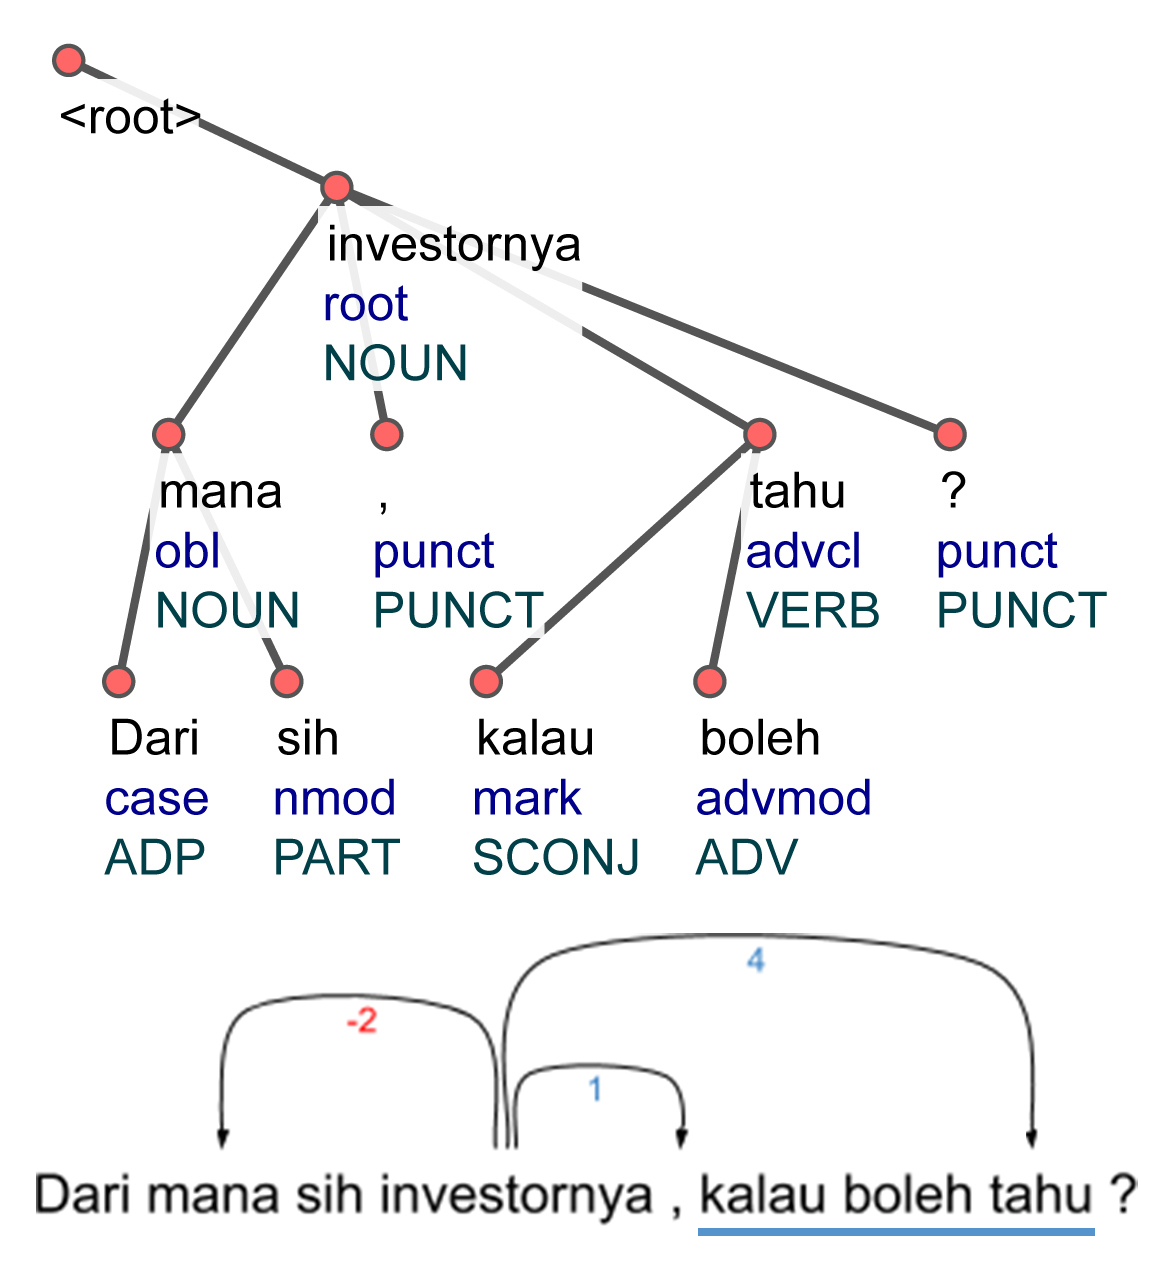
\includegraphics[width=1\linewidth] {pics/ls1436.jpg} 
	\caption{L\textit{akar}a}
	\label{fig:ls1436} 
\end{subfigure}
%
\begin{subfigure}{.58\linewidth}
  \centering
  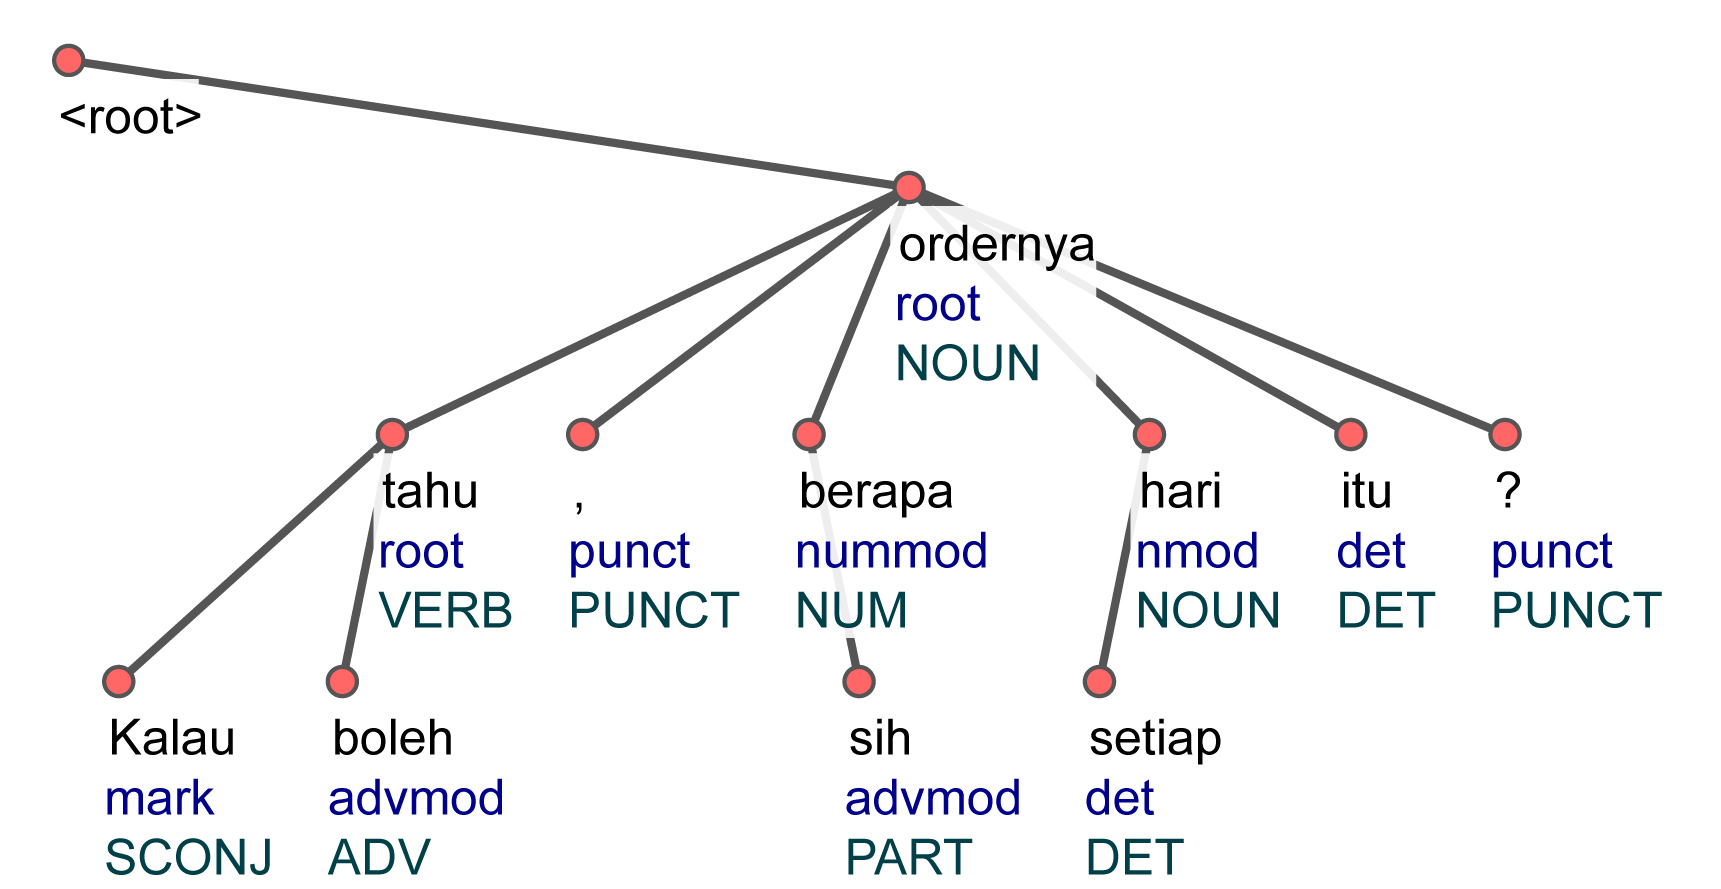
\includegraphics[width=1\linewidth]{pics/ls1460.jpg} 
	\caption{L\textit{akar}b}
	\label{fig:ls1460} 
\end{subfigure}

\caption{Contoh perbedaan penempatan klausa pada data ragam lisan}
\label{fig:akarcontoh}
\end{figure}


Salah satu bagian analisis penelitian ini berkaitan dengan valensi sebuah konstituen dalam kalimat. \pic~\ref{fig:akarcontoh} menampilkan contoh perbedaan penempatan klausa terikat \textit{kalau boleh tahu}. Sesuai dengan batasan penelitian ini, bagian analisis ini difokuskan hanya pada simpai pusat dengan kelas kata akar berupa kata kerja atau verba. \pic~\ref{fig:ls1436} dan \pic~\ref{fig:ls1460} merupakan dua kalimat yang ditemukan pada korpus data ragam lisan. Klausa terikat \textit{kalau boleh tahu} pada kalimat L\textit{akar}a (\pic~\ref{fig:ls1436}) dan L\textit{akar}b (\pic~\ref{fig:ls1460}) berada pada posisi yang berbeda namun tidak mengubah makna kalimat. Contoh serupa juga sempat dijabarkan oleh \cite{sneddon2010indonesian} dalam buku \textit{Indonesian Reference Grammar} Pada kalimat L\textit{akar}b, konstituen-konstiuen yang membentuk klausa \textit{kalau boleh tahu} secara kolektif memiliki relasi dependensi utama negatif terhadap akar \textit{ordernya}. Sesuai dengan bentuk relasi induk dan konstituen terikat berdasarkan teori dependensi yang dijabarkan oleh \cite{tesniere1959elements}, klausa terikat pada posisi awal kalimat ini harus disimpan dalam memori kerja terlebih dahulu hingga akar direalisasikan. Karena akar mengandung informasi utama, perbedaan kedua kalimat ini juga dapat memberikan sedikit gambaran bagaimana perbedaan proses memori kerja terkait penyimpanan informasi yang merupakan argumen inti kalimat.

\begin{figure}
\centering

\begin{subfigure}{.8\linewidth}
  \centering
  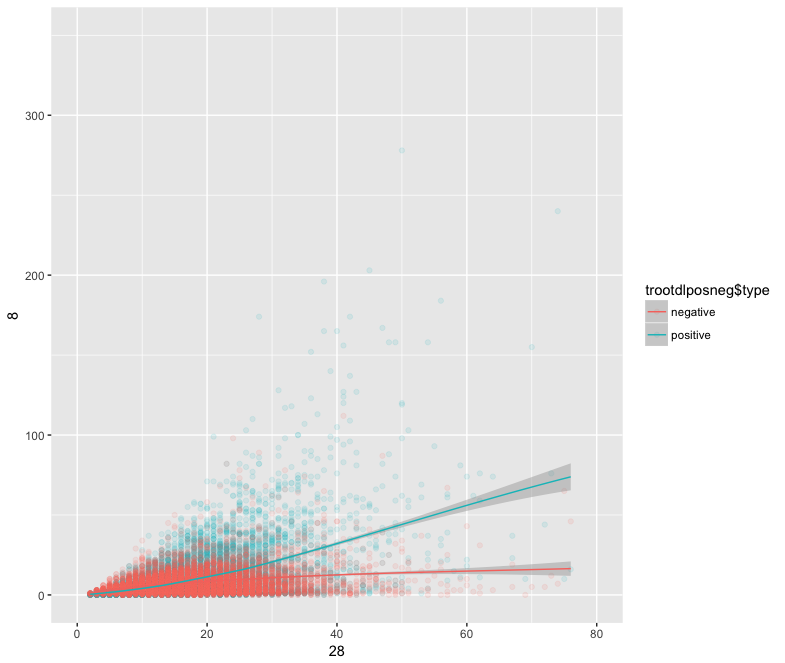
\includegraphics[width=1\linewidth] {pics/tulisroot_DLposneg.png} 
	\caption{Data ragam tulis}
	\label{fig:tulisroot_DLposneg} 
\end{subfigure}
%
\begin{subfigure}{.8\linewidth}
  \centering
  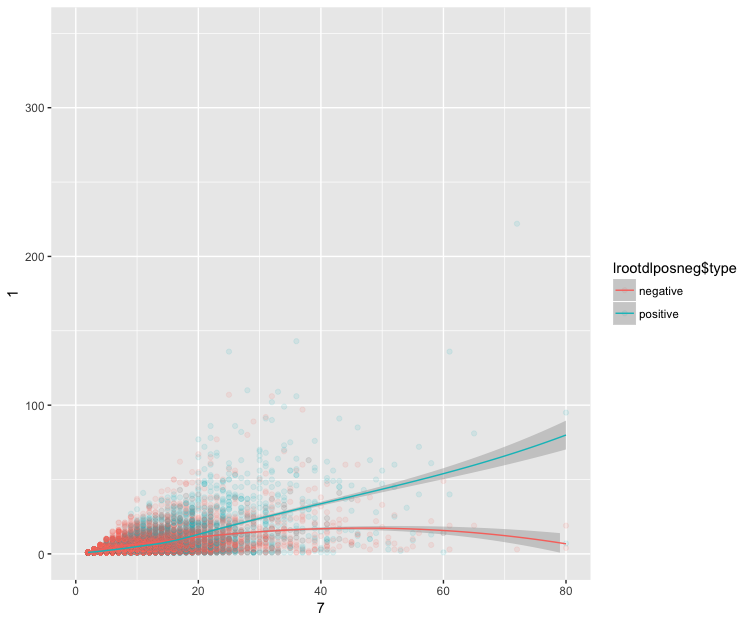
\includegraphics[width=1\linewidth]{pics/lisanroot_DLposneg.png} 
	\caption{Data ragam lisan}
	\label{fig:lisanroot_DLposneg} 
\end{subfigure}

\caption{Grafik panjang dependensi positif dan negatif pada simpai pusat data ragam tulis dan lisan}
\label{fig:rootDL_posneg}
\end{figure}

\pic~\ref{fig:tulisroot_DLposneg} dan \pic~\ref{fig:lisanroot_DLposneg} merupakan grafik DL positif dan negatif yang didapat pada simpai pusat kalimat dengan akar berupa verba. Kalimat dengan akar verbal ditemukan sebanyak 84,61\% atau sebanyak 7874 kalimat pada data ragam tulis dan 70,91\% atau sebanyak 7239 kalimat pada data ragam lisan. Mayoritas frekuensi kemunculan akar verbal ini dianalisis untuk melihat bagaimana penutur menyusun informasi utama dengan meninjau tautan-tautan dependensi utama (simpai pusat). Oleh sebab itu, semua klausa yang mungkin terikat pada simpai cabang dianggap mengikuti induknya seperti pada contoh uraian relasi klausa \textit{kalau boleh tahu} dan akarnya di atas (\pic~\ref{fig:akarcontoh}). \pic~\ref{fig:rootDL_posneg} menunjukkan adanya konsistensi pada tingkat tautan dependensi utama dan keseluruhan kalimat. Grafik ini memperlihatkan bahwa penutur juga cenderung memilih untuk menekan penggunaan bentuk relasi diakhiri induk terutama pada kalimat panjang. Berbeda dengan \pic~\ref{fig:DL_posneg} yang pada klasifikasi kalimat menengah sudah cukup terlihat perbedaan antara DL positif dan negatif, grafik ini menunjukkan DL positif dan negatif saling tumpang tindih sehingga perlu ditinjau lebih dalam. Meskipun begitu, serupa dengan \pic~\ref{fig:DL_posneg}, garis regresi nilai DL negatif mengindikasikan adanya ambang batas pada nilai tertentu terutama pada data ragam lisan.

\begin{table}
\begin{center}
\begin{small}
\caption{Frekuensi selisih panjang dependensi positif dan negatif pada simpai pusat akar verbal}  \label{tab:DLpusatposneg}
\begin{tabular}{ | p{2cm} | p{2cm} | p{2cm} | p{2cm} | p{2cm} |}
    \hline
Jumlah konstituen & Ragam tulis (+ \textgreater -) & Ragam tulis (+ \textless -) & Ragam lisan (+ \textgreater -) & Ragam lisan (+ \textless -) \\ \hline
\textless= 5 	& 57	 	& 180 	& 393 & 1008 \\ \hline
6 - 10 		& 475 	& 796	& 655 & 1356 \\ \hline
11 - 20 		& 1638	& 1804	& 964 & 1336 \\ \hline
21 - 30 		& 1028	& 778	& 384 & 291 \\ \hline
31 - 40 		& 325	& 177	& 121 & 85 \\ \hline
\textgreater 40 	& 137	& 37	 	& 61 & 30 \\ \hline
   \end{tabular}
   \end{small}
\end{center}
\end{table}

\tab~\ref{tab:DLpusatposneg} berisi jumlah-jumlah kalimat dengan melihat apakah kalimat tersebut memiliki DL postif yang lebih jauh atau sebaliknya pada simpai pusat yang memiliki akar verbal. Sebagai contoh, simpai pusat kalimat L4 \textit{Hasil surveynya cukup mengejutkan} pada \pic~\ref{fig:ls1102} memiliki 3 konstituen yang saling bertautan, yaitu \textit{mengejutkan} dengan \textit{hasil} dan \textit{mengejutkan} dengan \textit{cukup}. Kedua tautan memiliki bentuk relasi diakhiri induk dan memiliki DL negatif lebih jauh dibandingkan DL positif. Berbeda dengan \tab~\ref{tab:DLposneg}, kalimat yang DL positifnya lebih jauh ditemukan lebih banyak pada kalimat-kalimat panjang (mulai 21 konstituen). Pada ragam tulis, frekuensi keseluruhan hampir seimbang sedangkan pada ragam lisan cukup berbeda jauh (total frekuensi di mana DL negatif lebih jauh dari DL positif sebanyak dua kali lipat dibandingkan sebaliknya). 

\begin{table}
\begin{center}
\begin{small}
\caption{Frekuensi tautan dependensi positif dan negatif pada simpai pusat akar verbal}  \label{tab:tautanpusatposneg}
\begin{tabular}{ | p{2cm} | p{2cm} | p{2cm} | p{2cm} | p{2cm} |}
    \hline
Jumlah konstituen & Ragam tulis (+) & Ragam tulis (-) & Ragam lisan (+) & Ragam lisan (-) \\ \hline
\textless= 5 	& 201	& 412 & 1204 & 2151 \\ \hline
6 - 10 		& 1917	& 2532 & 2998 & 4433 \\ \hline
11 - 20 		& 6914 	& 7144 & 4753 & 5570 \\ \hline
21 - 30 		& 4455	& 3691 & 1869 & 1754 \\ \hline
31 - 40 		& 1528	& 1031 & 540 & 461 \\ \hline
\textgreater 40 	& 625	& 321 & 315 & 258 \\ \hline
   \end{tabular}
   \end{small}
\end{center}
\end{table}

\tab~\ref{tab:tautanpusatposneg} memperlihatkan bahwa pada simpai pusat akar verbal, kecenderungan untuk menggunakan bentuk relasi diawali induk juga baru terlihat pada panjang kalimat mulai 21 konstituen. Pada kalimat-kalimat yang lebih pendek dari itu, tautan dependensi negatif yang merepresentasikan bentuk relasi diakhiri induk justru lebih banyak. Pada data ragam tulis, total frekuensi dependensi negatif juga lebih banyak dibandingkan dependensi positif namun rasionya tidak seekstrim pada \tab~\ref{tab:DLpusatposneg}.

\begin{table}
\begin{center}
\begin{footnotesize}
\caption{Jarak dependensi seluruh tautan antarkonstituen pada simpai pusat akar verbal}  \label{tab:deskriptif-konstituenpusat}
\begin{tabular}{| c | llll | llll | l |}
\hline
 & \multicolumn{4}{c |}{+} & \multicolumn{4}{c |}{-} & \\  \cline{2-9}  
Panjang kalimat & min 	& med	& max 	& mean 	& min 	& med 	& max 	& mean 	& \\ \cline{1-10}  
\textless= 5 	& 1 		& 1 		& 3	 	& 1,428 	& 1 		& 1		& 4	 	& 1,748 	&\multirow{6}{*}{Tulis}\\
6 - 10 		& 1 		& 2		& 9	 	& 2,336 	& 1 		& 2	 	& 9	 	& 2,571 	& 	\\
11 - 20 		& 1 		& 3	 	& 18	 	& 4,083	& 1 		& 2	 	& 19	 	& 3,61 	& 	\\
21 - 30 		& 1 		& 4	 	& 27	 	& 6,265	& 1 		& 3 		& 29		& 4,793 	& 	\\ 
31 - 40 		& 1	 	& 6	 	& 38		& 9,046 	& 1 		& 3 		& 37		& 5,925 	& 	\\
\textgreater 40 	& 1	 	& 9		& 68	 	& 12,88 	& 1 		& 3 		& 44		& 6,791 	& 	\\ 
\hline
\textless= 5 	& 1 		& 1 		& 4	 	& 1,482 	& 1 		& 1	 	& 4		& 1,69 	& \multirow{6}{*}{Lisan}\\
6 - 10 		& 1 		& 2		& 9	 	& 2,28 	& 1 		& 2		& 9		& 2,618 	& \\
11 - 20 		& 1 		& 3 		& 19	 	& 3,826 	& 1 		& 2 		& 18		& 3,658 	& \\
21 - 30 		& 1	 	& 4	 	& 26	 	& 6,413	& 1 		& 3		& 27		& 4,789 	& \\ 
31 - 40 		& 1	 	& 6	 	& 35		& 8,638 	& 1 		& 4		& 32		& 6,505 	& \\
\textgreater 40 	& 1	 	& 7		& 66	 	& 10,27 	& 1	 	& 3		& 46		& 5,852 	& \\ 
\hline
   \end{tabular}
   \end{footnotesize}
\end{center}
\end{table}

\tab~\ref{tab:deskriptif-konstituenpusat} mencakup jarak dependensi dari seluruh tautan pada simpai pusat akar verbal dan tidak dikelompokkan berdasarkan kalimatnya. Tabel ini memperlihatkan bahwa rata-rata jarak dependensi positif lebih jauh dibandingkan dependensi negatif, terutama pada kalimat yang semakin panjang. Seperti pada \tab~\ref{tab:deskriptif-konstituen}, perbandingan ini mulai terlihat pada kategori panjang kalimat 11 konstituen dan meningkat seiring bertambahnya jumlah konstituen. Pada kategori kalimat terpanjang, perbandingan jarak antara dependensi positif dan negatif juga semakin jauh. Keserupaan temuan pada simpai pusat akar verbal dan pada keseluruhan kalimat (\tab~\ref{tab:deskriptif-konstituen}) menunjukkan bahwa meskipun dependensi negatif lebih banyak dari segi frekuensi (terutama pada ragam lisan), bahasa Indonesia tetap memperlihatkan penekanan terhadap nilai jarak dependensi negatif. Nilai tengah untuk semua ragam dan kategori panjang kalimat juga lebih mendekati ke nilai minimum, terutama pada ragam tulis. Pada kategori kalimat terpanjang ragam lisan (\textgreater 40 konstituen), rata-rata jarak dependensi negatif lebih pendek dibandingkan kategori sebelumnya (31-40 konstituen) dan perbedaan ini signifikan (\textit{P} \textless 0.05).  Serupa dengan \tab~\ref{tab:deskriptif-konstituen}, pada ragam lisan, mulai panjang kalimat tertentu (yang berdasarkan data ini adalah sekitar 40 konstituen) jarak dependensi negatif pada simpai pusat juga tidak akan melebihi nilai tertentu. 

\begin{table}
\begin{center}
\begin{footnotesize}
\caption{Rata-rata jarak dependensi positif dan negatif pada simpai pusat akar verbal}  \label{tab:deskriptif-mddpusat}
\begin{tabular}{| c | llll | llll | l |}
\hline
 & \multicolumn{4}{c |}{+} & \multicolumn{4}{c |}{-} & \\  \cline{2-9}  
Panjang kalimat & min 	& med	& max 	& mean 	& min 	& med 	& max 	& mean 	& \\ \cline{1-10}  
\textless= 5 	& 1 		& 1 		& 3	 	& 1,363	& 1 		& 1,5		& 4	 	& 1,632	&\multirow{6}{*}{Tulis}\\
6 - 10 		& 1 		& 2		& 7	 	& 2,091	& 1 		& 2	 	& 9	 	& 2,385	& 	\\
11 - 20 		& 1 		& 3	 	& 16	 	& 3,545	& 1 		& 2,75 	& 19	 	& 3,36 	& 	\\
21 - 30 		& 1 		& 5	 	& 19,5 	& 5,514	& 1 		& 3,333	& 28		& 4,442	& 	\\ 
31 - 40 		& 1	 	& 7,5	 	& 26		& 8,044	& 1 		& 4		& 36		& 5,448	& 	\\
\textgreater 40 	& 1	 	& 11,1	& 34,286	& 11,84	& 1 		& 4,2		& 42		& 6,264	& 	\\ 
\hline
\textless= 5 	& 1 		& 1 		& 3		& 1,327	& 1 		& 1,5 	& 4		& 1,531	& \multirow{6}{*}{Lisan}\\
6 - 10 		& 1 		& 1,667	& 5,6		& 1,801	& 1 		& 2		& 9		& 2,603	& \\
11 - 20 		& 1 		& 2,286	& 7,167	& 2,479	& 1 		& 2,125	& 6,818	& 2,315	& \\
21 - 30 		& 1,4	 	& 3,118	& 8,412	& 3,375	& 1 		& 2,182	& 8,636	& 2,460	& \\ 
31 - 40 		& 1,947	& 3,643	& 7,25	& 3,879	& 1 		& 2,353	& 7,5		& 2,688	& \\
\textgreater 40 	& 2,147	 & 4,051	& 8,697	& 4,156	& 1,059	& 2,357	& 5,053	& 2,47	& \\ 
\hline
   \end{tabular}
   \end{footnotesize}
\end{center}
\end{table}

Hasil pada \tab~\ref{tab:deskriptif-mddpusat} didapatkan dengan menghitung MDD positif dan negatif pada simpai pusat akar verbal setiap kalimat. Seperti \tab~\ref{tab:deskriptif-mdd}, distribusi nilai minimum, tengah dan maksimum pada ragam lisan juga lebih merata dibandingkan ragam tulis yang nilai tengahnya terlihat lebih mendekati nilai minimum terutama pada kalimat yang semakin panjang (mulai terlihat pada panjang kalimat 11 konstituen). Namun, perbedaannya terletak pada rata-rata MDD. Pada simpai pusat ini, rata-rata MDD ragam tulis jauh lebih besar dibandingkan ragam lisan. Seperti \tab~\ref{tab:deskriptif-konstituenpusat}, tabel ini juga memperlihatkan indikasi bahwa tautan dependensi negatif memiliki rata-rata jarak yang lebih pendek untuk kedua ragam. 

%%-----------------------------------------------------------------------------%
\subsection{Percabangan searah dan keseimbangan antara tautan dependensi positif dan negatif}
%%-----------------------------------------------------------------------------%
Pada tinjauan pustaka, pergerakan panah yang merepresentasikan direksionalitas induk dibahas menjadi dua tipe, yaitu percabangan searah (\textit{same-brancing}) dan percabangan beda arah (\textit{mixed-branching}) \citep{hawkins1994performance}. Namun, dengan jumlah konstituen yang semakin banyak dan kalimat yang semakin kompleks, direksionalitas induk tidak bisa digolongkan secara biner (hanya percabangan searah saja atau hanya percabangan beda arah saja) (\citealp{dryer1992greenbergian, temperley2008dependency}). \cite{gildea2010grammars} menjelaskan mengenai konsep keseimbangan antara tautan dependensi positif dan negatif dalam mendapatkan DL terpendek yang juga dianalisis oleh \citep{dryer1992greenbergian}. Berdasarkan data penelitian ini, temuan yang didapatkan mendukung asumsi yang dikemukakan \cite{dryer1992greenbergian} bahwa arah dependensi tidak bisa digolongkan secara biner pada tataran kalimat, terutama pada kalimat yang semakin panjang. Namun, berdasarkan analisis dengan pemetaan kepadatan selisih antara DL positif dan negatif, belum ditemukan kecenderungan terhadap bentuk keseimbangan tersebut. 

Pada ragam tulis, pemetaan kepadatan sangat menyebar sehingga tidak membentuk pola tertentu, sedangkan pada ragam lisan, pemetaan kepadatan terlalu memusat pada kalimat dengan jumlah konstituen sedikit sehingga juga tidak membentuk pola tertentu. Untuk mencari kecenderungan pada data seperti ini, perlu dilakukan pencarian fungsi matematis untuk menguji tingkat kesalahan (\textit{error rate}) yang lebih kecil antara kedua kemungkinan (percabangan searah atau keseimbangan dependensi positif dan negatif). Namun, pencarian fungsi matematis tersebut berada di luar batasan penelitian ini dan di luar ranah linguistik sehingga perlu dilakukan analisis lebih lanjut dari segi pembentukan model statistika. Asumsi sementara yang dapat diambil bertitik tolak dari grafik perbandingan DL positif dan negatif pada \pic~\ref{fig:DL_posneg} dan \pic~\ref{fig:rootDL_posneg} yang dapat memberikan gambaran adanya kecenderungan untuk menghindari tautan dependensi negatif, terutama pada kalimat yang semakin panjang.

%%-----------------------------------------------------------------------------%
\subsection{Akar pada posisi pertama dan klausa utama di awal kalimat tanpa pengurangan valensi}
%%-----------------------------------------------------------------------------%
Penempatan akar dan/atau klausa utama di awal kalimat tanpa mengurangi valensi verbal ditemukan pada kedua korpus data, terutama pada data ragam tulis. Penempatan akar verbal pada posisi pertama seperti kalimat T\textit{akar}a (\pic~\ref{fig:ts770}) dan T\textit{akar}b (\pic~\ref{fig:ts7458}) lebih banyak ditemukan pada korpus data ragam tulis klasifikasi kalimat pendek dan menengah. Sebaliknya, penempatan akar di posisi pertama tanpa mengurangi valensi verbal tersebut sangat jarang ditemukan pada data ragam lisan.

\begin{figure}
\centering
  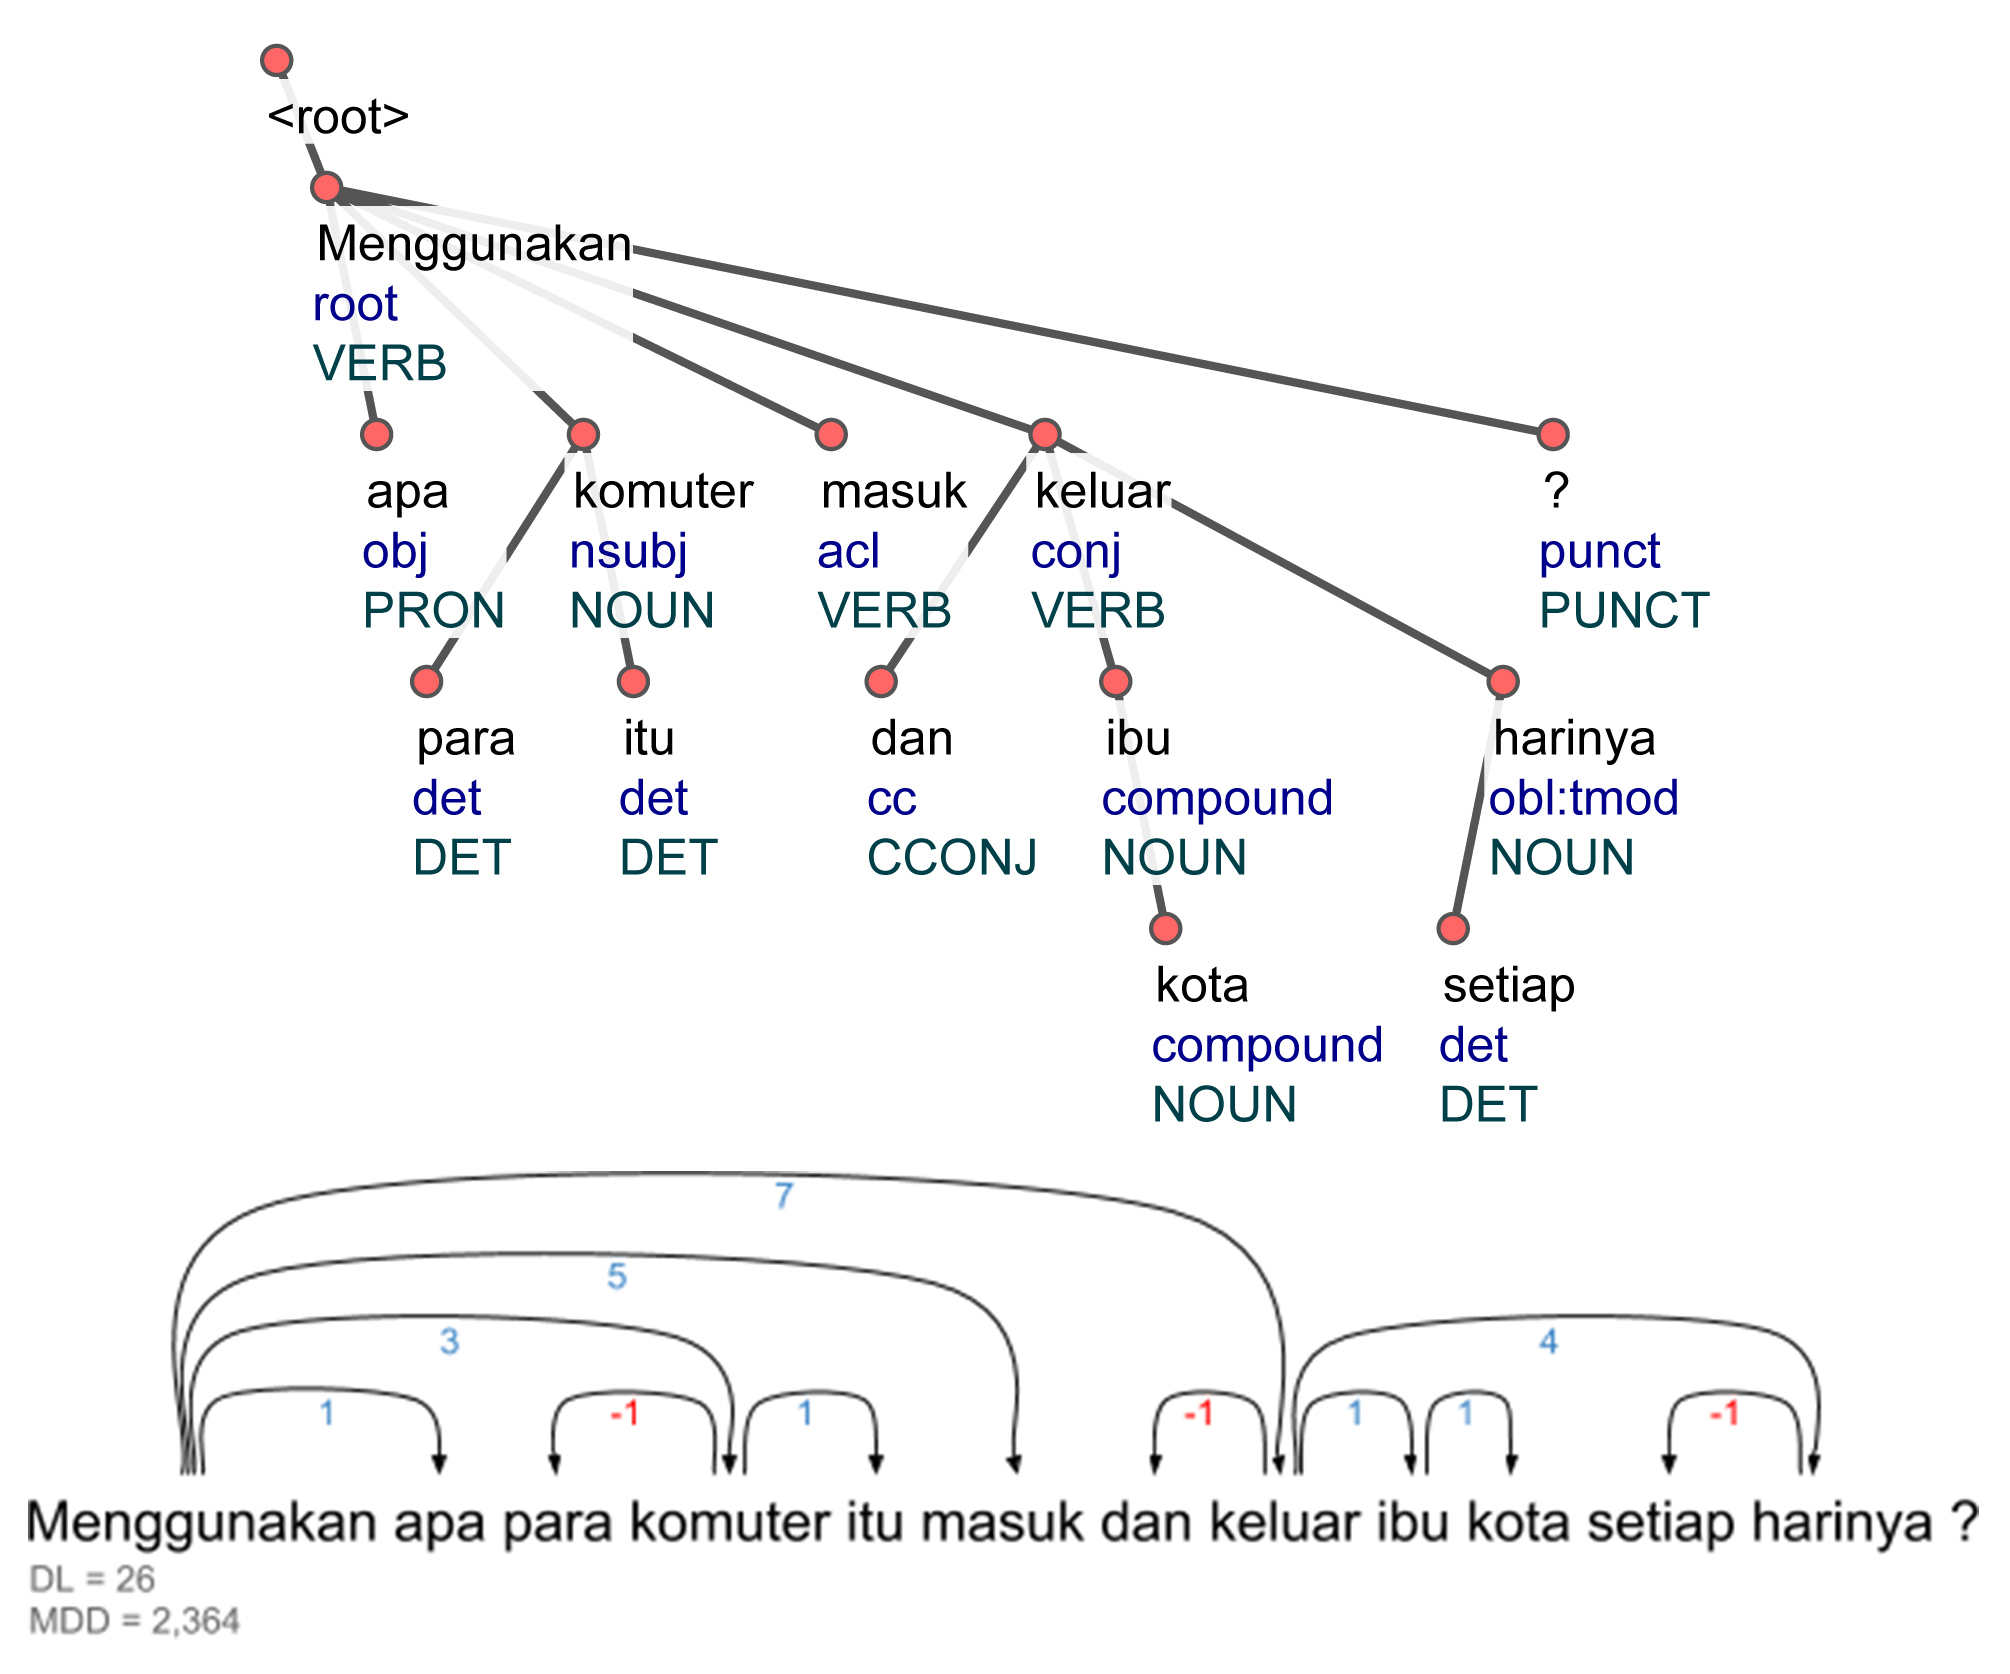
\includegraphics[width=.57\textwidth]{pics/ts7458.jpg} 
	\caption{Kalimat T\textit{akar}a pada data ragam tulis}
	\label{fig:ts7458} 
\end{figure}

Kalimat T\textit{akar}a (\pic~ref{fig:ts7458}) tetap mempertahankan valensi terhadap \textit{komuter} (aktor pelaku) dan \textit{apa} (pengganti obyek) namun konstruksinya tidak umum seperti halnya aktor pelaku mendahului verba dalam bahasa Indonesia. Contoh ini memberikan indikasi pemanfaatan kebebasan urutan kata dalam Bahasa Indonesia untuk menghindari bentuk relasi diakhiri induk dan tetap merealisasikan akar seawal mungkin. Penempatan klausa utama di awal kalimat lebih banyak ditemukan pada data ragam tulis dibandingkan ragam lisan. Penempatan klausa utama di awal kalimat ini menyebabkan akar verbal secara otomatis tetap berada di awal tanpa mengurangi valensi akar verbal tersebut. Namun, seiring jumlah konstituen yang semakin banyak dan struktur kalimat dengan klausa-klausa yang semakin kompleks, posisi akar verbal umumnya tidak pada posisi pertama meskipun masih pada rentang awal kalimat. Salah satu penyebab posisi akar sangat jarang ditemukan pada posisi pertama di kategori kalimat panjang adalah karena konstituen terikat berupa aktor pelaku umumnya direalisasikan sebelum akar verbal. Contoh strategi ini dapat dilihat pada kalimat T31b (\pic~\ref{fig:ts2081}) untuk data ragam tulis dan L31a (\pic~\ref{fig:ls1716}) untuk data ragam lisan.

%%-----------------------------------------------------------------------------%
\subsection{Pengurangan valensi akar pada klausa utama}
%%-----------------------------------------------------------------------------%
Sejumlah simpai pusat dalam kedua korpus data mengalami pengurangan valensi verbal yang mengakibatkan pengurangan panjang serta jarak dependensi. Hal ini berkaitan dengan temuan pengaruh panjang kalimat pada pembahasan sebelumnya yang menandakan kecenderungan jumlah konstituen yang lebih sedikit pada data ragam lisan. Strategi pengurangan valensi verbal ini juga ditemukan disertai penempatan akar di awal kalimat yang juga berkaitan dengan upaya menekan dependensi negatif yang berjarak jauh terutama pada kalimat panjang dalam data ragam lisan.

\begin{figure}
\centering

\begin{subfigure}{.49\linewidth}
  \centering
  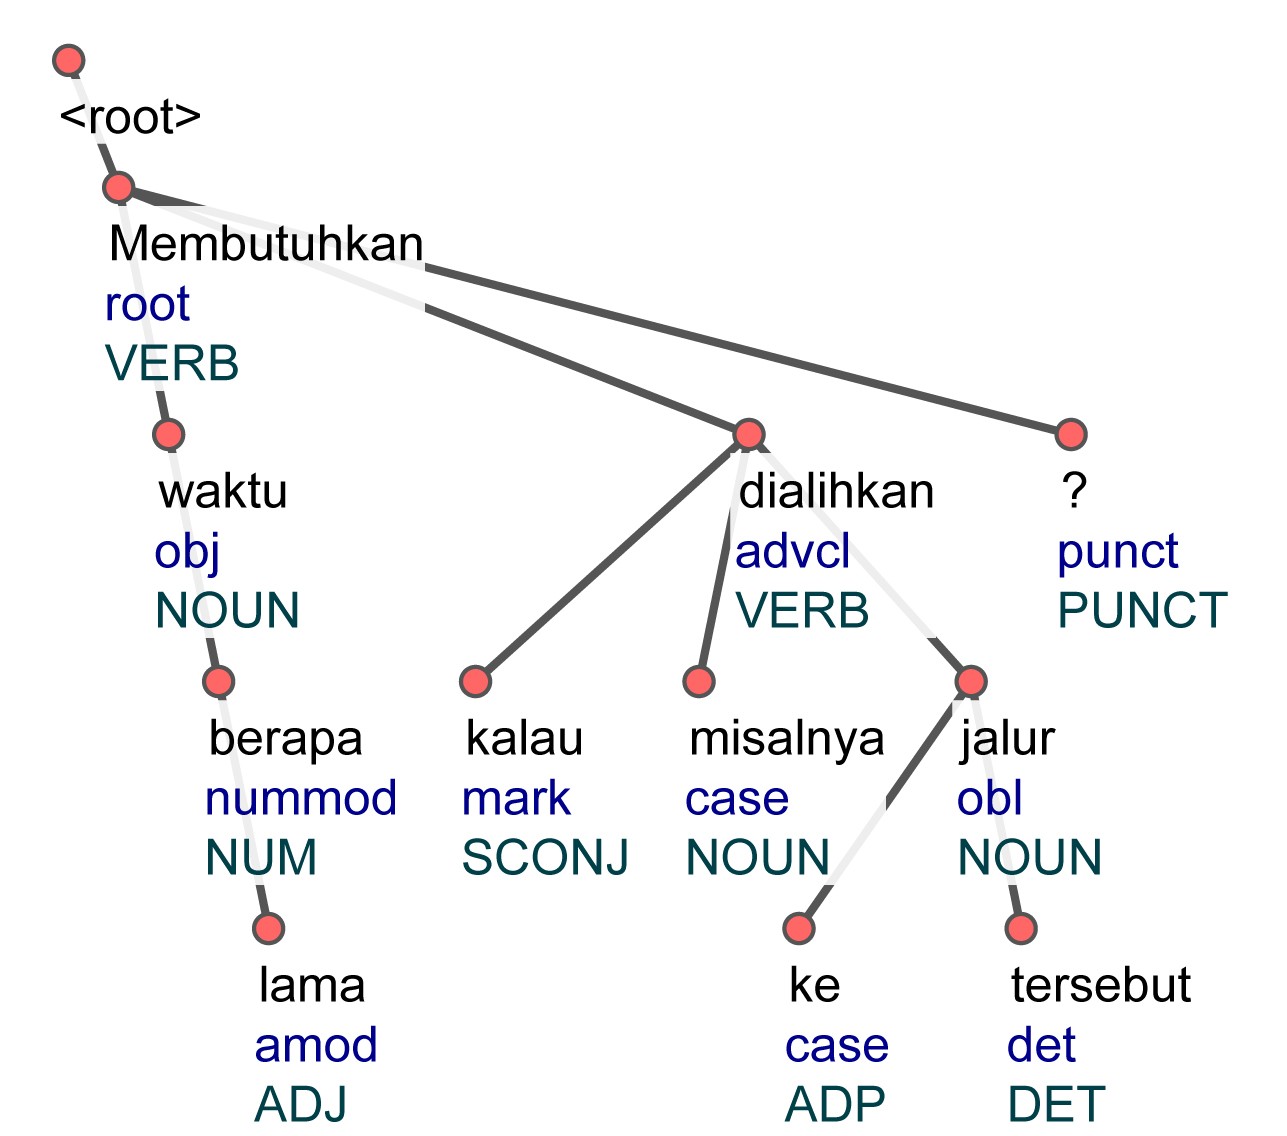
\includegraphics[width=1\linewidth] {pics/ls4820.jpg} 
	\caption{L\textit{akar}c}
	\label{fig:ls4820} 
\end{subfigure}
%
\begin{subfigure}{.41\linewidth}
  \centering
  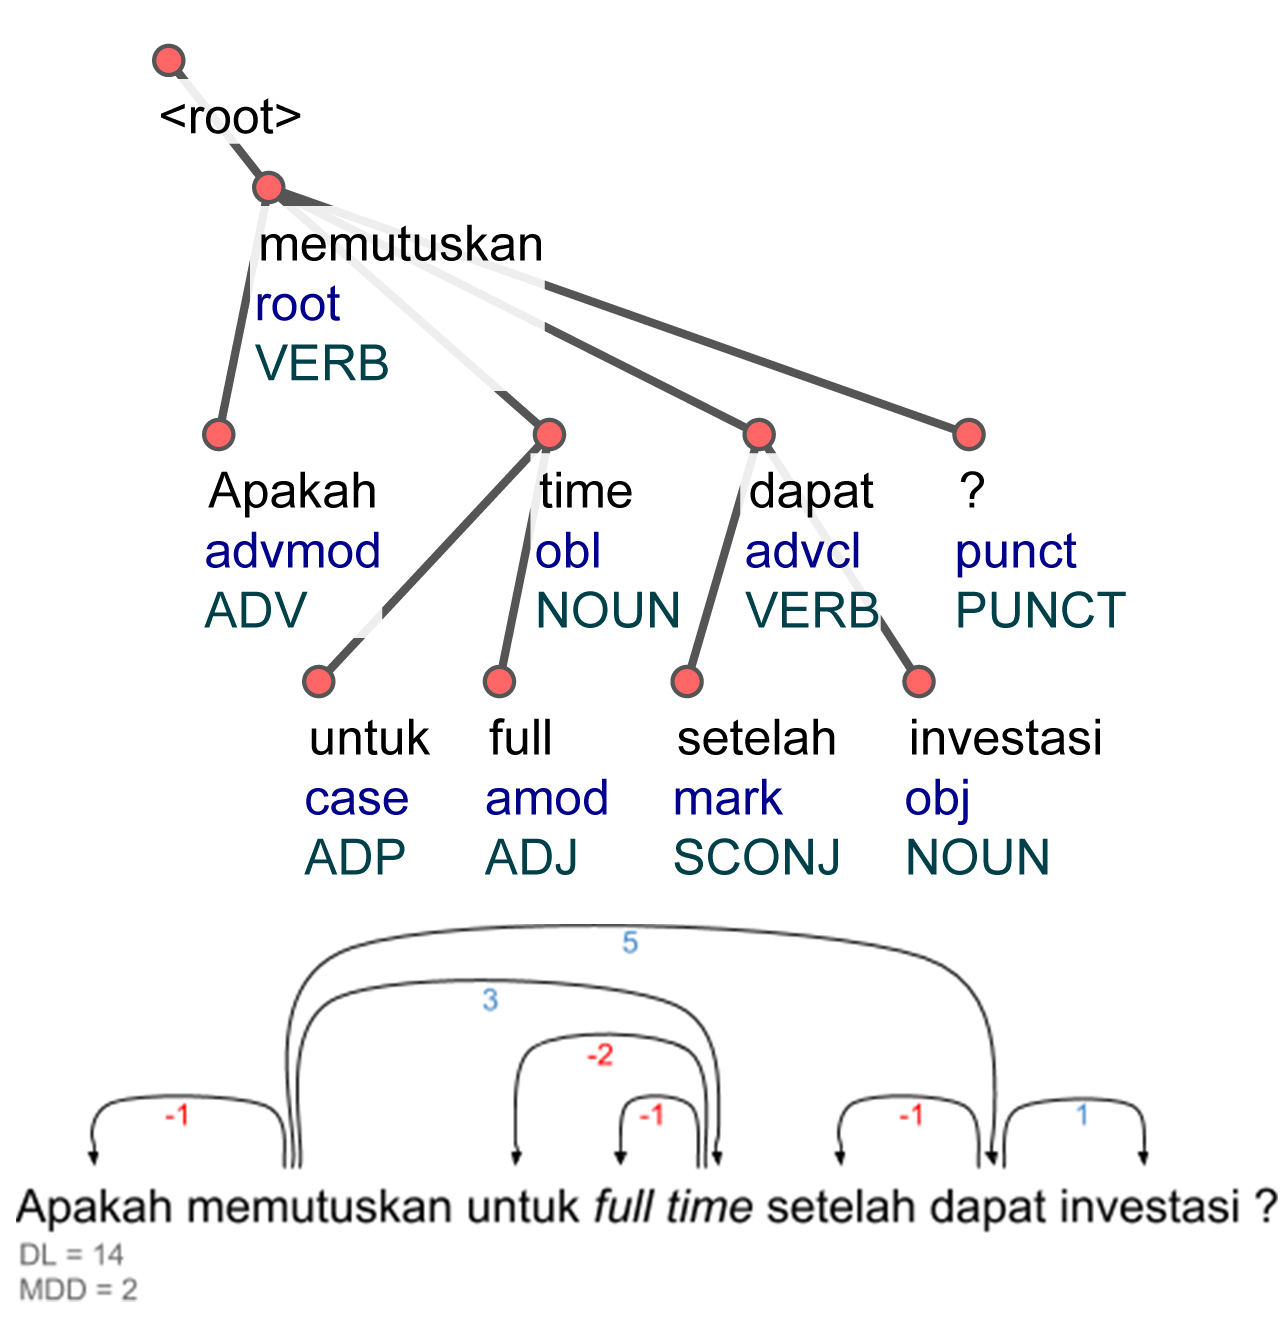
\includegraphics[width=1\linewidth]{pics/ls1435.jpg} 
	\caption{L\textit{akar}d}
	\label{fig:ls1435} 
\end{subfigure}
\caption{Contoh penempatan akar verbal dan klausa utama di awal kalimat tanpa pengurangan valensi verbal pada data ragam tulis}
\label{fig:rootvalensi}
\end{figure}

Pada kalimat L\textit{akar}c (\pic~\ref{fig:ls4820}), akar verbal \textit{membutuhkan} umumnya memiliki valensi sebanyak dua konstituen, yaitu aktor pelaku atau subyek berupa klausa dan obyek atau \textit{X membutuhkan Y}. Kata ini mengalami pengurangan valensi akar verbal sehingga yang muncul hanya obyek nomina \textit{waktu}. Meskipun demikian, akar \textit{membutuhkan} mengikat verba \textit{dialihkan} yang merupakan induk dari klausa keterangan. Pengurangan valensi pada data ragam lisan juga terjadi pada akar di posisi selain posisi pertama. Seperti pada kalimat L\textit{akar}d (\pic~\ref{fig:ls1435} yang juga mengalami pengurangan valensi berupa aktor pelaku untuk akar verbal \textit{memutuskan}. Kalimat L\textit{akar}e (\pic~\ref{fig:ls1265}), seperti juga kalimat L22 (\pic~\ref{fig:ls6521}), merupakan contoh yang mengalami pengurangan valensi verbal berupa aktor pelaku atau pronomina pada klausa utama maupun klausa terikatnya. Kalimat L\textit{akar}e tidak memunculkan pelengkap pada klausa \textit{X mengganti alat} dan/atau pada klausa \textit{supaya X tidak berebut ikan}.

\begin{figure}
	\centering 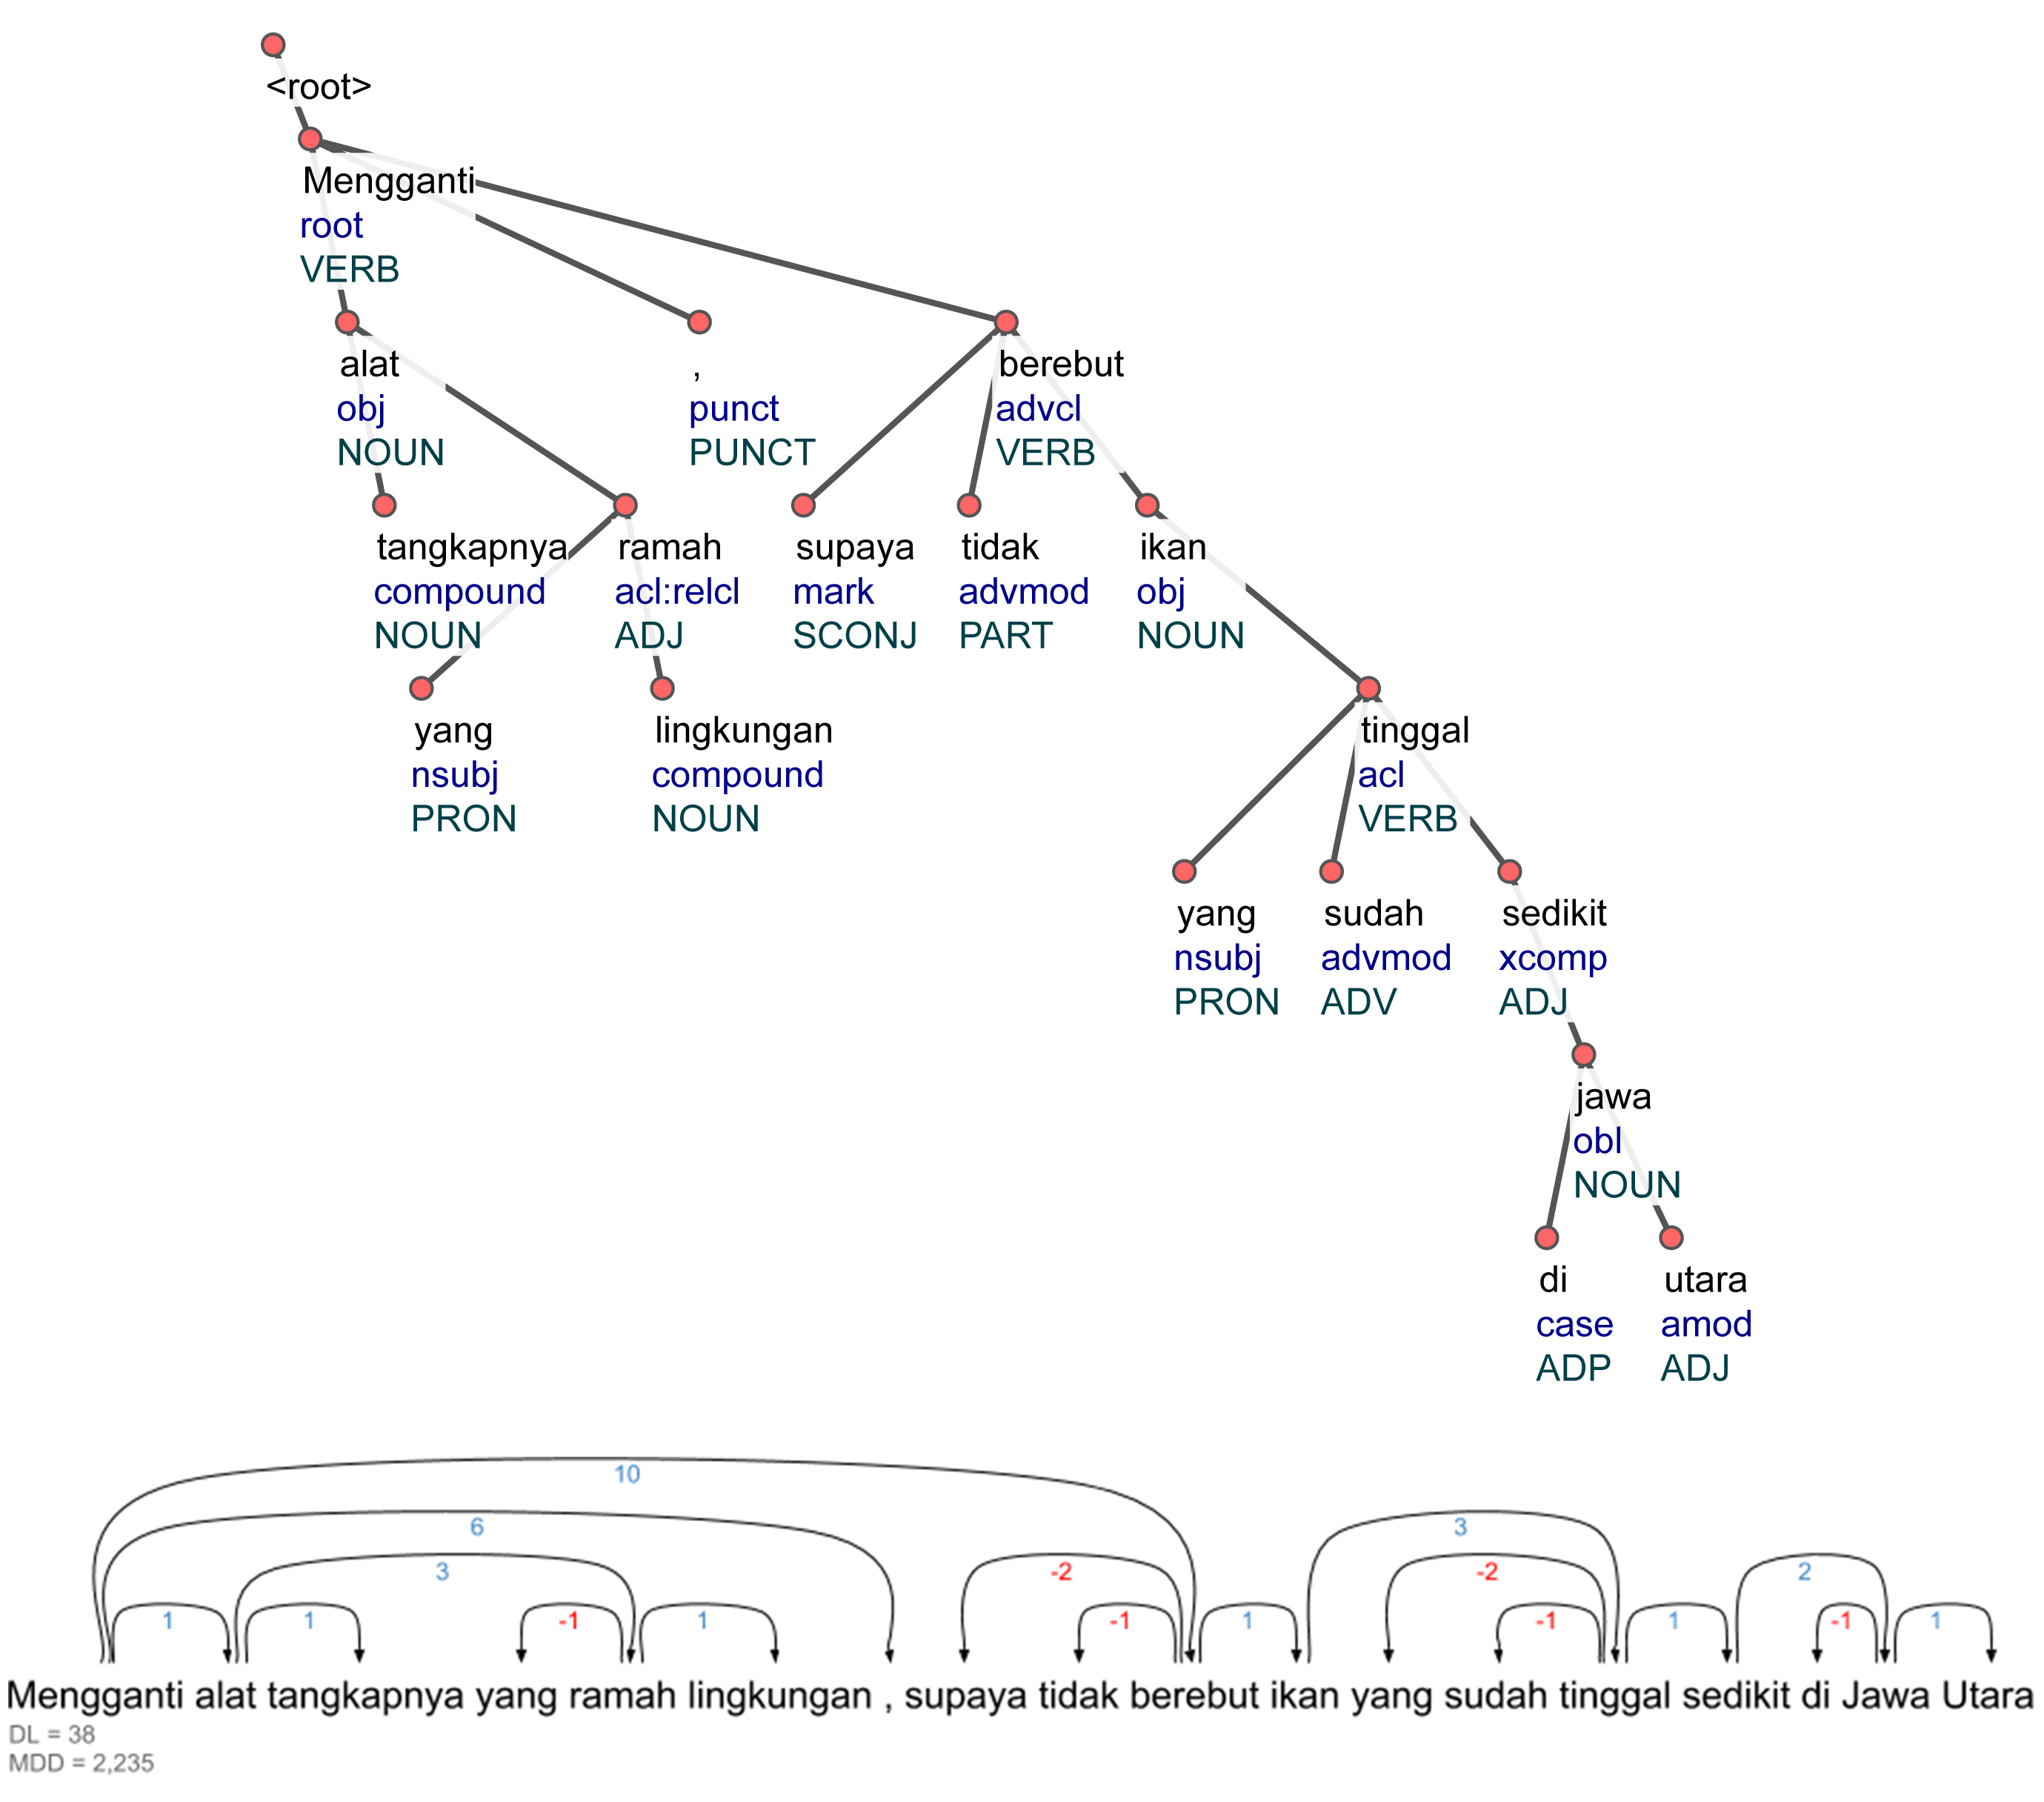
\includegraphics[width=0.9
	\textwidth] {pics/ls1265.jpg} 
	\caption{Kalimat L\textit{akar}e pada data ragam lisan}
	\label{fig:ls1265} 
\end{figure}

Strategi kalimat seperti ini muncul dalam wacana-wacana di mana konstituen yang direduksi dari valensi verbal sudah terlebih dahulu direalisasikan di kalimat-kalimat sebelumnya atau sudah dimengerti bersama tanpa harus direalisasikan dalam kalimat tertentu. Batasan penelitian ini hanya pada tataran kalimat sehingga tidak menganalisis hubungan dependensi yang terbentuk pada tataran wacana atau antarkalimat. Namun, asumsi ini menimbulkan pertanyaan untuk analisis dependensi lanjutan pada tataran wacana, yaitu bagaimana dan sejauh mana tautan dependensi yang terbentuk antarkalimat memungkinkan adanya pengurangan valensi verbal pada kalimat tertentu?

%%-----------------------------------------------------------------------------%
\subsection{Kecenderungan posisi induk terhadap konstituen terikat dalam kalimat}
%%-----------------------------------------------------------------------------%
Bagian analisis ini mencoba menjawab pertanyaan terkait direksionalitas induk atau arah tautan dependensi dan pengurangan valensi akar verbal pada simpai pusat. Pengurangan konstituen dalam kalimat atau preferensi terhadap kalimat pendek terutama pada ragam lisan tidak selalu berarti menandakan adanya pengurangan valensi sebuah konstituen. Pada penelitian-penelitian terdahulu banyak dilakukan eksplorasi terhadap reduksi leksikal lain seperti konjungsi, partikel, ataupun kata-kata lain yang bersifat berulang atau \textit{repetitive} (\citealp{jaeger2006redundancy, gildea2015human}). Penelitian ini memfokuskan pengurangan valensi pada simpai pusat dengan akar verbal yang merupakan tipe akar yang paling banyak ditemukan pada kedua korpus data. 

Seperti yang dibahas pada bab sebelumnya, direksionalitas induk dapat menyebabkan nilai dependensi tersebut menjadi positif atau negatif. Anotasi positif menandakan bentuk relasi induk sebelum konstituen terikat (diawali induk), sedangkan anotasi negatif menandakan bentuk relasi induk setelah konstituen terikat (diakhiri induk). Berdasarkan aturan struktur frasa dalam tata bahasa yang ada (\citealp{kridalaksana2002struktur, sneddon2010indonesian}), terdapat indikasi bahwa bahasa Indonesia tergolong bahasa yang memilih bentuk relasi diawali induk dibandingkan diakhiri induk atau \textit{head-final}. Namun, belum ada penelitian dengan skala cukup besar yang dapat memberikan informasi ini dengan memanfaatkan data tuturan nyata karena penerapannya dalam tuturan nyata dapat bersifat tidak gramatikal namun tetap diterima. Bentuk relasi diawali induk tidak selalu menjadi preferensi pada semua bahasa karena beberapa bahasa memiliki aturan tata bahasa yang menuntut induk muncul setelah konstituen terikat atau diakhiri induk. Meskipun belum ada konvensi dan bukti empiris yang menunjukkan bahwa bentuk diawali induk lebih memudahkan proses memori kerja, \cite{futrell2015large} menunjukkan bukti empiris bahwa bahasa-bahasa yang cenderung menggunakan bentuk relasi ini memiliki tingkat pengurangan jarak dependensi (DLM) lebih tinggi dibandingkan bahasa-bahasa yang cenderung menggunakan bentuk relasi diakhiri induk. 

Didukung oleh hasil penelitian ini, bahasa Indonesia menunjukkan kecenderungan terhadap bentuk relasi diawali induk pada keseluruhan kalimat (antarkonstituen yang memiliki tautan langsung) yang ditandai oleh konsistensi DL positif yang semakin besar dibandingkan DL negatif terutama pada kalimat yang memiliki jumlah konstituen lebih banyak. Namun, kecenderungan ini tidak terlalu jelas terlihat pada simpai pusat karena dari segi frekuensi, jumlah tautan dependensi negatif dan jumlah kalimat yang panjang dependensi negatifnya lebih besar ditemukan jauh lebih banyak terutama pada ragam lisan. Meskipun begitu, apabila jarak dependensi ikut diperhitungkan, terlihat adanya konsistensi untuk menekan panjang dan jarak dependensi negatif baik pada simpai pusat maupun keseluruhan kalimat. Secara otomatis, pergerakan DL positif yang semakin besar mengakibatkan penekanan bentuk relasi diakhiri induk yang ditandai oleh DL negatif. Bahkan, pada ragam lisan, ditemukan indikasi adanya ambang batas terhadap jarak dependensi untuk bentuk relasi diakhiri induk. Temuan ini memunculkan asumsi bahwa dalam bahasa Indonesia, bentuk relasi diawali induk lebih banyak digunakan penutur terutama pada relasi yang berjarak jauh. Hal ini juga menunjukkan indikasi bahwa bentuk ini lebih mudah diproduksi dan dipahami secara kognitif untuk penutur maupun penerima informasi. Penyebab adanya perbedaan kecenderungan frekuensi pada simpai pusat dan keseluruhan kalimat berkaitan dengan tinjauan kognitif dan persepsi manusia yang berada di luar batasan penelitian ini. Penelitian lebih lanjut yang dapat memperlihatkan bukti empiris dibutuhkan untuk mendukung hipotesis ini dan untuk mengukur seberapa besar dampak bentuk relasi diawali induk sehingga dapat memudahkan proses memori kerja. 

Analisis kualitatif untuk melihat lebih dalam bagaimana strategi yang mendukung preferensi bentuk relasi diawali induk ini dilakukan dengan meninjau simpai-simpai pusat kalimat yang memiliki akar verbal pada kedua korpus. Secara umum, ditemukan dua strategi terkait direksionalitas induk dan valensi akar verbal, yaitu penempatan akar dan klausa utama di awal kalimat dan pengurangan valensi akar verbal pada klausa utama. Penempatan akar dan klausa utama di awal kalimat sangat umum ditemukan pada semua klasifikasi dalam korpus data ragam tulis. Namun, posisinya sedikit bergeser ke tengah kalimat seiring dengan semakin banyaknya jumlah konstituen. Hal ini dikarenakan penempatan klausa utama yang hampir selalu berada di posisi awal kalimat pada data ragam tulis. Sementara, pengurangan valensi akar verbal hampir tidak ditemukan pada data ragam tulis yang mungkin disebabkan oleh karakter wacananya yang bersifat lebih formal dibandingkan dengan ragam lisan. 

Pengurangan valensi ini secara langsung berakibat pada pengurangan konstituen secara keseluruhan, sehingga dapat dikaitkan dengan temuan adanya preferensi untuk menggunakan kalimat dengan jumlah konstituen yang lebih sedikit pada ragam lisan, terutama pada klasifikasi kalimat pendek dan menengah. Beberapa kasus pengurangan valensi akar verbal ini juga ditemukan disertai dengan penempatan posisi akar di awal kalimat ragam lisan. Pada kasus yang lain, pengurangan valensi ini juga ditemukan pada klausa terikat di dalam kalimat tersebut. Mulai pada panjang kalimat tertentu, akar verbal yang mengikat aktor pelaku dalam valensinya tidak ditemukan pada posisi pertama dan aktor pelaku hampir selalu direalisasikan sebelum akar verbal atau didahului oleh konstituen dan klausa terikat. Pengurangan valensi subyek yang berupa kata penuh pada simpai pusat akar verbal tidak ditemukan apabila klausa utama didahului klausa lain, namun pengurangan valensi subyek yang berupa pronomina pengganti pada simpai dengan induk verbal ditemukan apabila klausa utama juga mengalami pengurangan valensi subyek. Untuk meninjau lebih dalam signifikansi temuan pengurangan valensi pada kondisi tersebut memerlukan pendekatan kuantitatif yang menuntut adanya sumber daya kamus atau leksikon valensi. Tinjauan lebih lanjut dengan memanfaatkan leksikon valensi dapat memberikan gambaran lebih dalam mengenai kognisi manusia terkait struktur kalimat yang dikonstruksi dan dapat memberikan masukan terhadap penggunaan tata bahasa yang memudahkan komunikasi serta proses memori kerja.

%%-----------------------------------------------------------------------------%
%\section{thesis.tex}
%%-----------------------------------------------------------------------------%
%Berkas ini berisi seluruh berkas Latex yang dibaca, jadi bisa dikatakan sebagai 
%berkas utama. Dari berkas ini kita dapat mengatur bab apa saja yang ingin 
%kita tampilkan dalam dokumen.
%
%
%%-----------------------------------------------------------------------------%
%\section{laporan\_setting.tex}
%%-----------------------------------------------------------------------------%
%Berkas ini berguna untuk mempermudah pembuatan beberapa template standar. 
%Anda diminta untuk menuliskan judul laporan, nama, npm, dan hal-hal lain yang 
%dibutuhkan untuk pembuatan template. 
%
%
%%-----------------------------------------------------------------------------%
%\section{istilah.tex}
%%-----------------------------------------------------------------------------%
%Berkas istilah digunakan untuk mencatat istilah-istilah yang digunakan. 
%Fungsinya hanya untuk memudahkan penulisan.
%Pada beberapa kasus, ada kata-kata yang harus selalu muncul dengan tercetak 
%miring atau tercetak tebal. 
%Dengan menjadikan kata-kata tersebut sebagai sebuah perintah \latex~tentu akan 
%mempercepat dan mempermudah pengerjaan laporan. 
%
%
%%-----------------------------------------------------------------------------%
%\section{hype.indonesia.tex}
%%-----------------------------------------------------------------------------%
%Berkas ini berisi cara pemenggalan beberapa kata dalam bahasa Indonesia. 
%\latex~memiliki algoritma untuk memenggal kata-kata sendiri, namun untuk 
%beberapa kasus algoritma ini memenggal dengan cara yang salah. 
%Untuk memperbaiki pemenggalan yang salah inilah cara pemenggalan yang benar 
%ditulis dalam berkas hype.indonesia.tex.
%
%
%%-----------------------------------------------------------------------------%
%\section{pustaka.tex}
%%-----------------------------------------------------------------------------%
%Berkas pustaka.tex berisi seluruh daftar referensi yang digunakan dalam 
%laporan. 
%Anda bisa membuat model daftar referensi lain dengan menggunakan bibtex.
%Untuk mempelajari bibtex lebih lanjut, silahkan buka 
%\url{http://www.bibtex.org/Format}. 
%Untuk merujuk pada salah satu referensi yang ada, gunakan perintah \bslash 
%cite, e.g. \bslash cite\{latex.intro\} yang akan akan memunculkan 
%\cite{latex.intro}
%
%
%%-----------------------------------------------------------------------------%
%\section{bab[1 - 6].tex}
%%-----------------------------------------------------------------------------%
%Berkas ini berisi isi laporan yang Anda tulis. 
%Setiap nama berkas e.g. bab1.tex merepresentasikan bab dimana tulisan tersebut 
%akan muncul. 
%Sebagai contoh, kode dimana tulisan ini dibaut berada dalam berkas dengan nama 
%bab4.tex. 
%Ada enam buah berkas yang telah disiapkan untuk mengakomodir enam bab dari 
%laporan Anda, diluar bab kesimpulan dan saran. 
%Jika Anda tidak membutuhkan sebanyak itu, silahkan hapus kode dalam berkas 
%thesis.tex yang memasukan berkas \latex~yang tidak dibutuhkan;  contohnya 
%perintah \bslash include\{bab6.tex\} merupakan kode untuk memasukan berkas 
%bab6.tex kedalam laporan.
%

%\include{bab5}
%\include{bab6}
%---------------------------------------------------------------
\chapter{\kesimpulan}
%---------------------------------------------------------------


%---------------------------------------------------------------
\section{Kesimpulan}
%---------------------------------------------------------------

Tinjauan terhadap pengurangan panjang dependensi (DLM) dan pengurangan jarak dependensi (DDM) pada tataran kalimat dalam bahasa Indonesia ragam tulis dan lisan memperlihatkan beberapa temuan yang sesuai prediksi. Temuan-temuan ini mendukung ide bahwa bahasa manusia memiliki kecenderungan untuk mengatur urutan kata sehingga memiliki panjang dependensi dan jarak dependensi yang pendek. Pendekatan ini dapat dilakukan dengan menerapkan beberapa strategi seperti yang telah dibahas pada penelitian-penelitian terdahulu (\citealp{jaeger2006redundancy, gildea2015human}). Dalam ranah sintaksis, strategi pendekatan-kata-kata ini termasuk melalui penyusunan urutan kata dan pengurangan kata dalam kalimat (yang mungkin diakibatkan oleh pengurangan unsur yang repetitif ataupun hal yang lain). 

Penelitian ini memanfaatkan dua metode untuk mengukur panjang dan jarak dependensi yaitu konsep panjang dependensi atau \textit{Dependency Length} (DL) dan rata-rata jarak dependensi atau \textit{Mean Dependency Distance} (MDD) untuk meninjau dua korpus yang berisikan teks informatif bahasa Indonesia dalam ragam tulis dan lisan. Kedua pendekatan ini memperlihatkan adaya perbedaan dalam temuan yang didapatkan terutama terkait pengaruh panjang kalimat terhadap panjang dan jarak dependensi. Hasil uji hipotesis dengan melakukan percobaan acak menggunakan \textit{Free Word Order Baseline} \citep{futrell2015large} yang menghasilkan 100 kemungkinan struktur kalimat yang tidak memiliki aturan urutan kata tertentu mendukung hipotesis bahwa terjadi DLM pada kedua korpus data (ragam tulis maupun ragam lisan) secara signifikan (\textit{P} \textless 0,001). 

Analisis kemungkinan pengaruh panjang kalimat terhadap panjang dan jarak dependensi serta penyusunan struktur kalimat menghasilkan temuan yang menunjukkan indikasi adanya kondisi tertentu di mana panjang kalimat berpengaruh secara signifikan dan kondisi lain di mana pengaruh tersebut tidak terlalu jelas. Kedua pendekatan DL dan MDD menunjukkan signifikansi pada kategori kalimat pendek, terutama pada jumlah konstituen 5 atau kurang, dan pada kalimat panjang, terutama pada jumlah konstituen antara 21 hingga 30. Namun, perbedaan yang didapat dengan menerapkan pendekatan DL tidak signifikan selain kedua kategori tersebut. Bahasa Indonesia ragam lisan memperlihatkan kecenderungan yang kuat untuk mengurangi panjan kalimat dalam menghasilkan panjang dan jarak dependensi yang pendek. Dari hasil tinjauan yang lebih dekat dan hasil analisis kualiltatif terhadap struktur sintaktis beberapa kalimat contoh, pengurangan panjang dan jarak dependensi pada ragam lisan ini diakibatkan terutama oleh reduksi elemen sintaktis yang termasuk didalamnya reduksi atau pengurangan valensi kata. Temuan ini juga sempat disinggung oleh \cite{jaeger2006redundancy} yang meneliti reduksi sintaktis  pada ujaran spontan dalam bahasa Inggris. Dalam bahasa Indonesia, hal ini mungkin berkaitan dengan karakteristik bahasa Indonesia yang cukup bebas terkait penerapan tata bahasa dalam ujaran nyata \citep{sneddon2010indonesian} dan urutan kata yang bebas \citealp{sneddon2010indonesian, kridalaksana2002struktur}. 

Meskipun bahasa Indonesia ragam tulis menunjukkan distribusi panjang kalimat yang lebih merata, ragam ini menghasilkan panjang dan jarak dependensi terkecil pada jumlah konstituen yang lebih banyak (terindikasi mulai dari 6 konstituen, tapi menunjukkan signifikansi tinggi pada jumlah konstituen lebih dari 20). Tinjauan lebih dekat dan hasil analisis kualitatif terhadap struktur sintaktis beberapa kalimat contoh mendukung temuan tersebut dan bahkan memperlihatkan manifestasi karakteristik sintaktis yang mungkin ditemukan eksklusif terhadap masing-masing ragam. Hal ini berarti, dilihat dari konstruksi kalimatnya, kalimat pada ragam tulis dan lisan memiliki ciri-ciri tersendiri. Sehingga, reduksi konstituen merupakan strategi yang lebih diutamakan pada ragam lisan. Keseluruhan tinjauan terkait panjang kalimat ini menunjukkan adanya indikasi bahwa tata bahasa dalam bahasa Indonesia yang diterapkan dalam teks dengan karakter yang lebih formal mendukung hipotesis DLM dan DDM. 

Dalam teori struktur frasa, bahasa Indonesia memiliki banyak hubungan di mana kata kepala berada di posisi sebelum kata yang memodifikasinya. Namun, hubungan ini umumnya hanya menjelaskan frasa yang terdiri dari kata-kata yang saling berdampingan. Dependensi melihat hubungan induk dengan konstituen terikat tidak hanya pada level tersebut, tapi juga hingga pada level argumen utama. Analisis direksionalitas induk yang dilakukan penelitian ini juga menunjukkan kesesuaian hierarki hubungan dalam struktur frasa tersebut baik pada level kata-kata yang berdampingan hingga pada level argumen utama (yang terlihat pada simpai pusat). Temuan ini menjadi bukti empiris adanya kecenderungan terhadap bentuk relasi diawali induk pada bahasa Indonesia, terutama pada ragam tulis. Namun, berdasarkan pemetaan dan visualisasi, kecenderungan antara bahasa Indonesia memanfaatkan strategi percabangan searah dengan strategi menyeimbangkan nilai dependensi positif dan negatif belum terpapar dengan jelas. Penelitian lebih lanjut yang melibatkan pencarian tingkat kesalahan (\textit{margin of error}) dengan fungsi matematis perlu dilakukan untuk menjawab pertanyaan ini. Meskipun begitu, analisis kualitatif terhadap kalimat-kalimat panjang dalam ragam tulis memperlihatkan banyaknya relasi dependensi yang berdampingan sehingga menunjukkan adanya indikasi bahwa kalimat-kalimat panjang dalam bahasa Indonesia ragam tulis menerapkan strategi percabangan searah.

Dari sisi tata bahasa, temuan pada ragam lisan juga memperlihatkan bagaimana ragam ini menyimpang dari tata bahasa yang ada dan struktur sintaktis yang tidak konsisten. Hal ini mungkin disebabkan oleh keterbatasan kognisi manusia untuk merealisasikan kalimat secara verbal, terutama untuk kalimat panjang. Temuan ini juga memiliki keterkaitan terhadap reduksi konstituen dalam upaya untuk menghasilkan panjang dan jarak dependensi yang pendek. Data ragam lisan tidak menunjukkan kecenderungan secara signifikan terhadap bentuk relasi diawali induk dari segi frekuensi, namun memperlihatkan kecenderungan signifikan untuk menekan jauh jarak dependensi yang negatif. Hal ini menimbulkan pertanyaan bahwa apakah strategi terkait direksionalitas induk tidak selalu menjadi preferensi penutur untuk menghasilkan kalimat yang efisien atau ini merupakan salah satu karakteristik ragam lisan yang tidak konsisten.

Pada ragam lisan, banyak kalimat ditemukan tidak memiliki aktor pelaku atau subyek pada argumen utama berdasarkan pada analisis valensi akar verbal pada simpai pusat di beberapa kalimat ragam lisan. Penelitian ini mengambil prinsip dasar dalam konsep kemungkinan pola valensi atau \textit{Probabilistic Valency Pattern} (PVP) \citep{liu2006syntactic} untuk analisis kualitatif. Kalimat seperti ini banyak ditemukan terutama pada panjang kalimat pendek dan menengah. Meskipun jarang ditemukan pada kalimat panjang, terdapat temuan yang cukup menarik. Apabila argumen utama (pada klausa utama) tidak memiliki aktor pelaku, pronomina yang merujuk pada aktor pelaku tersebut juga tidak ditemukan pada klausa terikat. Namun, apabila pronomina ditemukan pada klausa terikat, klausa utama juga memunculkan aktor pelaku. 

Secara umum, berdasarkan data yang dikumpulkan, bahasa Indonesia ragam tulis dan lisan memiliki perbedaan karakteristik dalam mengonstruksikan struktur sintaktis untuk menghasilkan kalimat yang efisien dari segi dependensi. Bahasa Indonesia ragam lisan lebih menunjukkan kecenderungan untuk mengurangi konsituen dalam kalimat dan menghasilkan kalimat yang pendek. Sebaliknya, kalimat yang lebih panjang dalam ragam tulis menunjukkan konstruksi sintaktis yang lebih terorganisir dibandingkan ragam lisan. Hal ini mungkin disebabkan oleh keterbatasan memori kerja manusia dalam memproduksi kalimat panjang secara verbal. Untuk mendapatkan pemahaman mengenai konstruksi yang lebih efisien secara akurat dan yang lebih mendekati preferensi pendengar, beberapa penelitian lanjutan perlu dilakukan. Meskipun begitu, penelitian ini telah memberikan dasar awal yang fundamental untuk dapat dikembangkan menjadi penelitian-penelitian linguistik transdisipliner lain terhadap keterkaitan struktur sintaktis sebuah kalimat dengan keterbatasan memori kerja dalam kognisi manusia.

%---------------------------------------------------------------
\section{Perkembangan Penelitian}
%---------------------------------------------------------------

Temuan yang berlawanan dalam data bahasa Indonesia ragam tulis dan lisan pada kalimat pendek dan panjang memunculkan beberapa pertanyaan untuk penelitian-penelitian lanjutan. Perbedaan struktur sintaktis akibat konstruksi kalimat kedua ragam memicu tinjauan lanjutan untuk mengukur struktur sintaktis secara kuantitatif dan akurat dalam usaha lebih mengerti mengenai tuntutan sintaktis dalam kognisi manusia. Terkait dengan valensi, penelitian ini belum mengukur secara akurat dan mengkuantifikasi analisis valensi karena kamus atau leksikon valensi dalam bahasa Indonesia belum ada. Sementara, konsep PVP \citep{liu2006syntactic} yang dimanfaatkan dalam penelitian ini dan analisis valensi dalam beberapa bahasa lain telah sampai pada analisis kuantitatif berskala besar dan pembentukan leksikon valensi terutama valensi verbal (\citealp{zabokrtsky2005valency, bielicky2008building, passarotti2016latin, semecky2006constructing}). Sehingga, leksikon valensi terutama untuk verba dalam bahasa Indonesia penting untuk dikembangkan dalam upaya untuk mendapatkan analisis valensi yang lebih mendalam terkait kemampuan sebuah kata untuk mengikat kata lain. 

Penelitian lanjutan yang melibatkan uji persepsi untuk meninjau ada tidaknya preferensi pendengar atau pembaca terhadap struktur sintaktis tertentu juga akan memberikan masukan wawasan linguistik yang sangat bermanfaat dalam mempelajari penampilan linguistik dalam bahasa Indonesia. Kajian lain juga dibutuhkan untuk dapat membuktikan apakah perbedaan ini bersifat kontekstual terhadap bahasa Indonesia atau bersifat lintas bahasa. Aspek penting lainnya yang perlu ditinjau adalah kemungkinan adanya perbedaan tingkat pemahaman bahasa antara pendengar (yang mendengar kalimat secara verbal) dan pembaca (yang membaca kalimat secara tertulis) yang dapat mempengaruhi pandangan terhadap struktur sintaktis mana yang lebih dipahami. 

%
% Daftar Pustaka
%
% Daftar Pustaka 
% 

% 
% Tambahkan pustaka yang digunakan setelah perintah berikut. 
% 
%\phantomsection %hack to add clickable section for pustaka
%\begin{thebibliography}{4}
%
%\bibitem{latex.intro}
%{Jeff Clark. (n.d). \f{Introduction to LaTeX}.
%26 Januari 2010. \url{http://frodo.elon.edu/tutorial/tutorial/node3.html}.}
%
%\end{thebibliography}


\bibliographystyle{apacite}
\bibliography{pustaka}


%
% Lampiran 
%
\begin{appendix}
	\include{markLampiran}
	\setcounter{page}{2}
	%Lampiran merupakan data atau pelengkap atau hasil olahan yang menunjang penulisan tugas akhir, tetapi tidak dicantumkan di dalam isi tugas akhir, karena akan mengganggu kesinambungan pembacaan. Lampiran yang perlu disertakan dikelompokkan menurut jenisnya, antara lain jadwal, tabel, daftar pertanyaan, gambar, grafik, desain. Pengelompokan lampiran disesuaikan dengan kebijakan fakultas.

%Ketentuan pembuatan lampiran adalah sebagai berikut.
%a. Nomor dan judul lampiran ditulis di sudut kanan atas halaman (right-aligned) dengan huruf tegak tipe Times New Roman 12 poin.
%b. Judul lampiran ditik dalam satu baris menggunakan huruf kapital di awal kata (titlecase).
%c. Lampiran yang lebih dari satu halaman, pada halaman berikutnya diberi keterangan ?lanjutan? dalam tanda kurung pada sudut kanan atas halaman (right-aligned).
%d. Isi dan urutan pengelompokan lampiran disesuaikan dengan kebijakan fakultas


%-----------------------------------------------------------------------------%
\addChapter{Contoh bank pohon struktur dependensi ragam tulis}
\chapter*{Lampiran 1: Contoh Bank Pohon Struktur Dependensi Ragam Tulis}
%-----------------------------------------------------------------------------%

\begin{figure}
	\centering \includegraphics[width=0.35
	\textwidth] {pics/lampiran/lampirants770.jpg} 
	\caption{Bank pohon struktur dependensi ragam tulis dokumen 770} 
	\label{fig:lampirants770} 
\end{figure}

\begin{figure}
	\centering \includegraphics[width=0.3
	\textwidth] {pics/lampiran/lampirants1956.jpg} 
	\caption{Bank pohon struktur dependensi ragam tulis dokumen 1956} 
	\label{fig:lampirants1956} 
\end{figure}

\begin{figure}
	\centering \includegraphics[width=0.15
	\textwidth] {pics/lampiran/lampirants2537.jpg} 
	\caption{Bank pohon struktur dependensi ragam tulis dokumen 2537} 
	\label{fig:lampirants2537} 
\end{figure}

\begin{figure}
	\centering \includegraphics[width=0.8
	\textwidth] {pics/lampiran/lampirants2624.jpg} 
	\caption{Bank pohon struktur dependensi ragam tulis dokumen 2624} 
	\label{fig:lampirants2624} 
\end{figure}

\begin{figure}
	\centering \includegraphics[width=0.8
	\textwidth] {pics/lampiran/lampirants3221.jpg} 
	\caption{Bank pohon struktur dependensi ragam tulis dokumen 3221} 
	\label{fig:lampirants3221} 
\end{figure}

%%

\begin{figure}
	\centering \includegraphics[width=0.45
	\textwidth] {pics/lampiran/lampirants4955.jpg} 
	\caption{Bank pohon struktur dependensi ragam tulis dokumen 4955} 
	\label{fig:lampirants4955} 
\end{figure}

\begin{figure}
	\centering \includegraphics[width=0.8
	\textwidth] {pics/lampiran/lampirants5360.jpg} 
	\caption{Bank pohon struktur dependensi ragam tulis dokumen 5360} 
	\label{fig:lampirants5360} 
\end{figure}

\begin{figure}
	\centering \includegraphics[width=0.25
	\textwidth] {pics/lampiran/lampirants5385.jpg} 
	\caption{Bank pohon struktur dependensi ragam tulis dokumen 5385} 
	\label{fig:lampirants5385} 
\end{figure}

\begin{figure}
	\centering \includegraphics[width=0.7
	\textwidth] {pics/lampiran/lampirants6703.jpg} 
	\caption{Bank pohon struktur dependensi ragam tulis dokumen 6703} 
	\label{fig:lampirants6703} 
\end{figure}

\begin{figure}
	\centering \includegraphics[width=0.45
	\textwidth] {pics/lampiran/lampirants7706.jpg} 
	\caption{Bank pohon struktur dependensi ragam tulis dokumen 7706} 
	\label{fig:lampirants7706} 
\end{figure}

%%

\begin{figure}
	\centering \includegraphics[width=0.4
	\textwidth] {pics/lampiran/lampirants8990.jpg} 
	\caption{Bank pohon struktur dependensi ragam tulis dokumen 8990} 
	\label{fig:lampirants8990} 
\end{figure}

\begin{figure}
	\centering \includegraphics[width=0.5
	\textwidth] {pics/lampiran/lampirants9184.jpg} 
	\caption{Bank pohon struktur dependensi ragam tulis dokumen 9184} 
	\label{fig:lampirants9184} 
\end{figure}


%-----------------------------------------------------------------------------%
\addChapter{Contoh bank pohon struktur dependensi ragam lisan}
\chapter*{Lampiran 2: Contoh Bank Pohon Struktur Dependensi Ragam Lisan}
%-----------------------------------------------------------------------------%

\begin{figure}
	\centering \includegraphics[width=0.4
	\textwidth] {pics/lampiran/lampiranls100.jpg} 
	\caption{Bank pohon struktur dependensi ragam lisan dokumen 100} 
	\label{fig:lampiranls100} 
\end{figure}

\begin{figure}
	\centering \includegraphics[width=0.6
	\textwidth] {pics/lampiran/lampiranls592.jpg} 
	\caption{Bank pohon struktur dependensi ragam lisan dokumen 592} 
	\label{fig:lampiranls592} 
\end{figure}

\begin{figure}
	\centering \includegraphics[width=0.4
	\textwidth] {pics/lampiran/lampiranls1100.jpg} 
	\caption{Bank pohon struktur dependensi ragam lisan dokumen 1100} 
	\label{fig:lampiranls1100} 
\end{figure}

\begin{figure}
	\centering \includegraphics[width=0.45
	\textwidth] {pics/lampiran/lampiranls1836.jpg} 
	\caption{Bank pohon struktur dependensi ragam lisan dokumen 1836} 
	\label{fig:lampiranls1836} 
\end{figure}

\begin{figure}
	\centering \includegraphics[width=0.3
	\textwidth] {pics/lampiran/lampiranls1928.jpg} 
	\caption{Bank pohon struktur dependensi ragam lisan dokumen 1928} 
	\label{fig:lampiranls1928} 
\end{figure}

%%

\begin{figure}
	\centering \includegraphics[width=0.45
	\textwidth] {pics/lampiran/lampiranls3530.jpg} 
	\caption{Bank pohon struktur dependensi ragam lisan dokumen 3530} 
	\label{fig:lampiranls3530} 
\end{figure}

\begin{figure}
	\centering \includegraphics[width=0.5
	\textwidth] {pics/lampiran/lampiranls4327.jpg} 
	\caption{Bank pohon struktur dependensi ragam lisan dokumen 4327} 
	\label{fig:lampiranls4327} 
\end{figure}

\begin{figure}
	\centering \includegraphics[width=0.45
	\textwidth] {pics/lampiran/lampiranls4991.jpg} 
	\caption{Bank pohon struktur dependensi ragam lisan dokumen 4991} 
	\label{fig:lampiranls4991} 
\end{figure}

\begin{figure}
	\centering \includegraphics[width=0.6
	\textwidth] {pics/lampiran/lampiranls5677.jpg} 
	\caption{Bank pohon struktur dependensi ragam lisan dokumen 5677} 
	\label{fig:lampiranls5677} 
\end{figure}

\begin{figure}
	\centering \includegraphics[width=0.5
	\textwidth] {pics/lampiran/lampiranls7047.jpg} 
	\caption{Bank pohon struktur dependensi ragam lisan dokumen 7047} 
	\label{fig:lampiranls7047} 
\end{figure}

%%

\begin{figure}
	\centering \includegraphics[width=0.35
	\textwidth] {pics/lampiran/lampiranls7359.jpg} 
	\caption{Bank pohon struktur dependensi ragam lisan dokumen 7359} 
	\label{fig:lampiranls7359} 
\end{figure}

\begin{figure}
	\centering \includegraphics[width=0.5
	\textwidth] {pics/lampiran/lampiranls7375.jpg} 
	\caption{Bank pohon struktur dependensi ragam lisan dokumen 7375} 
	\label{fig:lampiranls7375} 
\end{figure}


\end{appendix}

\end{document}
